% !TeX program = lualatex
\documentclass[fleqn]{NotesClass}

\let\mywidetilde\widetilde
\AtBeginDocument{\let\widetilde\mywidetilde}

\strictpagecheck

%% Packages
\usepackage{csquotes}
\usepackage{siunitx}
\usepackage{subcaption}

\usepackage{slashed}
\declareslashed{}{\not}{.1}{.5}{A}
\declareslashed{}{\not}{.05}{.5}{p}
\declareslashed{}{\not}{.1}{.5}{\partial}
\declareslashed{}{\not}{-.05}{.6}{q}
\declareslashed{}{\not}{-.1}{.5}{a}
\declareslashed{}{\not}{0.05}{.5}{W}

\usepackage{multienum}
\usepackage{tensor}
\usepackage{mhchem}

\newenvironment{multiitem}{%
    \multienumerate\renewcommand{\labelname}{\textbullet}%
}{%
    \endmultienumerate%
}

% Tikz stuff
\usepackage{tikz}
%\tikzset{>=latex}
% £xternal
\usetikzlibrary{external}
\tikzexternalize[prefix=tikz-external/]
% Other libraries
\usetikzlibrary{angles}
\usetikzlibrary{quotes}
\usetikzlibrary{arrows.meta}

\usepackage[compat=1.1.0]{tikz-feynman}

\usepackage{pgfplots}
\pgfplotsset{compat=1.18}

% References, should be last things loaded
\usepackage[pdfauthor={Willoughby Seago},pdftitle={Particle Physics},pdfkeywords={particle physics, Feynman diagrams, scattering, Dirac equation, QED, QCD, weak interactions},pdfsubject={particle physics}]{hyperref}  % Should be loaded second last (cleveref last)
\colorlet{hyperrefcolor}{blue!60!black}
\hypersetup{colorlinks=true, linkcolor=hyperrefcolor, urlcolor=hyperrefcolor, citecolor=hyperrefcolor}
\usepackage[
capitalize,
nameinlink,
noabbrev
]{cleveref} % Should be loaded last

% My packages
\usepackage{NotesBoxes}
\usepackage{NotesMaths}

\setmathfont[range={\int, \oint}]{Latin Modern Math}

% Highlight colour
\definecolor{Burgandy}{HTML}{8F2D56}
\definecolor{Teal}{HTML}{218380}
\definecolor{Blue}{HTML}{73D2DE}
\definecolor{Pink}{HTML}{D81159}
\definecolor{Yellow}{HTML}{FFBC42}

\colorlet{highlight}{Burgandy}

\usepackage{xcolor-solarized}

\lstMakeShortInline[style=mathematica, basicstyle=\color{solarized-base02}]£

\lstset{upquote}

\lstdefinestyle{mathematica}{
    language=mathematica,
    basicstyle=\color{solarized-base02}
}

\lstset{
    literate=
    {->}{{\(\to\)}}{2}
}

% Title page info
\title{Particle Physics}
\author{Willoughby Seago}
\date{September 20th, 2022}
% \subtitle{}
% \subsubtitle{}

% Open Question environment ---------------------------------------------------
\BeforeBeginEnvironment{openquestion}{%
    \vspace*{0pt plus 3pt} % To help with underfull vbox warnings
    \refstepcounter{equation}%
}

\AfterEndEnvironment{openquestion}{%
    \vspace*{0pt plus 3pt} % To help with underfull vbox warnings
}

\newtcbtheorem[number freestyle={\noexpand\theequation},%
crefname={Open Question}{Open Questions}]%
{openquestion}{Open Question}%
{enhanced jigsaw,%
    enforce breakable,%
    shrink break goal=0.5\baselineskip,%
    segmentation style=solid,%
    theorem style=plain,%
    %    before title app={{\tiny\ensuremath{\blacksquare}}\nobreakspace},%
    fonttitle=\sffamily\upshape\bfseries\small,%
    coltitle=black,%
    description font=\sffamily\upshape\bfseries\small,%
    description color=black,%
    colframe=highlight,%
    colback=azure(web)(azuremist)!45,%
    boxrule=0pt,%
    leftrule=4pt,%
    sharp corners,%
    description delimiters={}{},%
    separator sign={\nobreakspace {\color{black}---}},%
    terminator sign={\ },%
    label type=app,%
    label separator=,
}{}
% End application environment -----------------------------------------------

% Commands

\definecolor{redgluoncolor}{HTML}{7d0421}
\definecolor{bluegluoncolor}{HTML}{000099}
\definecolor{greengluoncolor}{HTML}{127d04}
\definecolor{antiredgluoncolor}{HTML}{00DEDE}
\definecolor{antigreengluoncolor}{HTML}{DE00DE}
\definecolor{antibluegluoncolor}{HTML}{FFD700}


% Particles
\newcommand{\Pparticle}[1]{\symup{#1}}
\newcommand{\Pu}{\ensuremath{\Pparticle{u}}}
\newcommand{\Pd}{\ensuremath{\Pparticle{d}}}
\newcommand{\Ps}{\ensuremath{\Pparticle{s}}}
\newcommand{\Pc}{\ensuremath{\Pparticle{c}}}
\newcommand{\Pt}{\ensuremath{\Pparticle{t}}}
\newcommand{\Pb}{\ensuremath{\Pparticle{b}}}
\newcommand{\Pe}{\ensuremath{\Pparticle{e}^{-}}}
\newcommand{\Penominus}{\ensuremath{\Pparticle{e}}}
\newcommand{\Pmu}{\ensuremath{\text{\normalfont μ}^{-}}}
\newcommand{\Pmunominus}{\ensuremath{\text{\normalfont μ}}}
\newcommand{\Ptau}{\ensuremath{\text{\normalfont τ}^{-}}}
\newcommand{\Ptaunominus}{\ensuremath{\text{\normalfont τ}}}
\newcommand{\Pnue}{\ensuremath{\text{\normalfont ν}_{\symup{e}}}}
\newcommand{\Pnumu}{\ensuremath{\text{\normalfont ν}_{\text{μ}}}}
\newcommand{\Pnutau}{\ensuremath{\text{\normalfont ν}_{\text{τ}}}}
\newcommand{\Pnuone}{\ensuremath{\upnu_{1}}}
\newcommand{\Pnutwo}{\ensuremath{\upnu_{2}}}
\newcommand{\Pnuthree}{\ensuremath{\upnu_{3}}}
\newcommand{\PH}{\ensuremath{\Pparticle{H}}}
\newcommand{\PZ}{\ensuremath{\Pparticle{Z}}}
\newcommand{\PW}{\ensuremath{\Pparticle{W}}}
\newcommand{\PWpm}{\ensuremath{\Pparticle{W}^{\pm}}}
\newcommand{\PWp}{\ensuremath{\Pparticle{W}^{+}}}
\newcommand{\PWm}{\ensuremath{\Pparticle{W}^{-}}}
\newcommand{\Pphoton}{\ensuremath{\text{\normalfont γ}}}
\newcommand{\Pg}{\ensuremath{\Pparticle{g}}}
\newcommand{\Pq}{\ensuremath{\Pparticle{q}}}
\newcommand{\Ppi}{\ensuremath{\text{\normalfont π}}}
\newcommand{\Ppip}{\ensuremath{\text{\normalfont π}^{+}}}
\newcommand{\Ppim}{\ensuremath{\text{\normalfont π}^{-}}}
\newcommand{\Ppizero}{\ensuremath{\text{\normalfont π}^{0}}}
\newcommand{\Prhozero}{\ensuremath{\text{\normalfont ρ}^{0}}}
\newcommand{\Pf}{\ensuremath{\Pparticle{f}}}
\newcommand{\Pred}{\ensuremath{\mathcolor{redgluoncolor}{\Pparticle{r}}}}
\newcommand{\Pgreen}{\ensuremath{\mathcolor{greengluoncolor}{\Pparticle{g}}}}
\newcommand{\Pblue}{\ensuremath{\mathcolor{bluegluoncolor}{\Pparticle{b}}}}
\newcommand{\PJpsi}{\ensuremath{\Pparticle{J}/\text{\normalfont ψ}}}
\newcommand{\Pp}{\ensuremath{\Pparticle{p}}}
\newcommand{\PKm}{\ensuremath{\Pparticle{K}^-}}
\newcommand{\PKp}{\ensuremath{\Pparticle{K}^+}}
\newcommand{\PKzero}{\ensuremath{\Pparticle{K}^0}}
\newcommand{\PK}{\ensuremath{\Pparticle{K}}}
\newcommand{\PKshort}{\ensuremath{\Pparticle{K}_{\symrm{S}}}}
\newcommand{\PKlong}{\ensuremath{\Pparticle{K}_{\symrm{L}}}}
\newcommand{\PBzerodown}{\ensuremath{\Pparticle{B}^0_{\Pd}}}
\newcommand{\PBzerostrange}{\ensuremath{\Pparticle{B}^0_{\Ps}}}
\newcommand{\PB}{\ensuremath{\Pparticle{B}}}
\newcommand{\PDzero}{\ensuremath{\Pparticle{D}^0}}
\newcommand{\Phiggs}{\ensuremath{\Pparticle{H}}}


\newcommand{\APantiparticle}[1]{\overbar{#1}}
\newcommand{\APu}{\ensuremath{\APantiparticle{\Pparticle{u}}}}
\newcommand{\APd}{\ensuremath{\APantiparticle{\Pparticle{d}}}}
\newcommand{\APs}{\ensuremath{\APantiparticle{\Pparticle{s}}}}
\newcommand{\APc}{\ensuremath{\APantiparticle{\Pparticle{c}}}}
\newcommand{\APt}{\ensuremath{\APantiparticle{\Pparticle{t}}}}
\newcommand{\APb}{\ensuremath{\APantiparticle{\Pparticle{b}}}}
\newcommand{\APe}{\ensuremath{\Pparticle{e}^{+}}}
\newcommand{\APmu}{\ensuremath{\text{\normalfont μ}^{+}}}
\newcommand{\APtau}{\ensuremath{\text{\normalfont τ}^{+}}}
\newcommand{\APnue}{\ensuremath{\APantiparticle{\text{\normalfont ν}}_{\symup{e}}}}
\newcommand{\APnumu}{\ensuremath{\APantiparticle{\text{\normalfont ν}}_{\text{μ}}}}
\newcommand{\APnutau}{\ensuremath{\APantiparticle{\text{\normalfont ν}}_{\text{τ}}}}
\newcommand{\APH}{\ensuremath{\Pparticle{H}}}
\newcommand{\APZ}{\ensuremath{\Pparticle{Z}}}
\newcommand{\APWpm}{\ensuremath{\Pparticle{W}^{\mp}}}
\newcommand{\APWp}{\ensuremath{\Pparticle{W}^{-}}}
\newcommand{\APWm}{\ensuremath{\Pparticle{W}^{+}}}
\newcommand{\APphoton}{\ensuremath{\text{\normalfont γ}}}
\newcommand{\APg}{\ensuremath{\Pparticle{g}}}
\newcommand{\APq}{\ensuremath{\APantiparticle{\Pparticle{q}}}}
\newcommand{\APf}{\ensuremath{\APantiparticle{\Pparticle{f}}}}
\newcommand{\APred}{\ensuremath{\textcolor{antiredgluoncolor}{\APantiparticle{\Pparticle{r}}}}}
\newcommand{\APgreen}{\ensuremath{\textcolor{antigreengluoncolor}{\APantiparticle{\Pparticle{g}}}}}
\newcommand{\APblue}{\ensuremath{\textcolor{antibluegluoncolor}{\APantiparticle{\Pparticle{b}}}}}
\newcommand{\APKzero}{\ensuremath{\APantiparticle{\Pparticle{K}}^0}}
\newcommand{\APBzerodown}{\ensuremath{\APantiparticle{\Pparticle{B}}^0_{\Pd}}}
\newcommand{\APBzerostrange}{\ensuremath{\APantiparticle{\Pparticle{B}}^0_{\Ps}}}
\newcommand{\APDzero}{\ensuremath{\APantiparticle{\Pparticle{D}}^0}}
\newcommand{\APp}{\APantiparticle{\Pparticle{p}}}

% Text
\newcommand{\course}[1]{\textit{#1}}

% Maths
\newcommand{\strongCoupling}{g_{\symrm{s}}}
\newcommand{\wCoupling}{g_{\symrm{W}}}
\newcommand{\zCoupling}{g_{\symrm{Z}}}
\newcommand{\EM}{\text{EM}}
\newcommand{\strongForce}{\symrm{S}}
\newcommand{\e}{\symrm{e}}
\newcommand{\probability}{\symbb{P}}
\DeclareMathOperator{\sinc}{sinc}
\newcommand{\amplitude}{\symcal{M}}
\newcommand{\dalembertian}{\partial^2}
\DeclarePairedDelimiterX{\anticommutator}[2]{\{}{\}}{#1 , #2}
\newcommand{\hermit}{\dagger}
\newcommand{\minkowskiSpace}{\reals^{1,3}}
\newcommand{\diracadjoint}[1]{\overbar{#1}}
\newcommand{\dirac}{\symup{D}}
\newcommand{\minkowskiMetric}{\eta}
\newcommand{\lagrangianDensity}{\symcal{L}}
\newcommand{\trans}{\top}
\newcommand{\ident}{\symbb{1}}
\newcommand{\Left}{\symrm{L}}
\newcommand{\Right}{\symrm{R}}
\newcommand{\parity}{\symcal{P}}
\newcommand{\chargeConjugation}{\symcal{C}}
\newcommand{\timeReversal}{\symcal{T}}
\DeclarePairedDelimiterX{\commutator}[2]{[}{]}{#1, #2}
\newcommand{\numberofcolors}{N_{\symrm{c}}}
\newcommand{\fermiConstant}{G_{\symrm{F}}}
\DeclareMathOperator{\BR}{BR}
\newcommand{\cabibboAngle}{\vartheta_{\symrm{c}}}
\newcommand{\boltzmann}{k_{\symrm{B}}}
\newcommand{\rep}[1]{\symbf{#1}}
\newcommand{\lagrangian}{L}

\includeonly{parts/appParticleData, parts/appFermiGoldenRule, parts/appPolarisation, parts/appFeynCalc}

\begin{document}
    \frontmatter
    \titlepage
    \innertitlepage{tikz-external/standard-model}
    \tableofcontents
    \listoffigures
    \mainmatter
    
    \chapter{Preliminaries}
    This course is not interested in the finer mathematical details, but the broader principles.
    For details see the \course{Quantum Field Theory} course.
    Knowledge is assumed of quantum mechanics (see the \course{Principles of Quantum Mechanics} and \course{Quantum Theory} courses), and special relativity (see the \course{Relativity, Nuclear, and Particle Physics} course, or \course{Classical Electrodynamics}).
    
    We use natural units where \(c = \hbar = \varepsilon_0 = \mu_0 = 1\).
    This means that masses, momentums, and energies are all measured in electron volts, force in electron volts squared, lengths and times in inverse electron volts, and speeds and angular momentums are dimensionless.
    Electric charge is also dimensionless, but the charge of an electron is  \emph{not} set to unity, although particle charges are given in terms of the (absolute value of the) electron charges.
    Instead we have the fine structure constant,
    \begin{equation}
        \alpha = \frac{e^2}{4\pi \varepsilon_0 \hbar c} \quad (\text{SI}) \qquad \alpha = \frac{e^2}{4\pi} \quad (c = \hbar = \varepsilon_0 = 1).
    \end{equation}
    The charge of an electron then has magnitude
    \begin{equation}
        e = \sqrt{4\pi \alpha}.
    \end{equation}
    Since \(\alpha\) is dimensionless its value is the same in any system of units, and is approximately \(1/137\), so
    \begin{equation}
        e \approx \num{0.303}.
    \end{equation}
    
    We use the Minkowski metric with the \(({+}{-}{-}{-})\) convention:
    \begin{equation}
        \eta_{\mu\nu} = \eta^{\mu\nu} = 
        \begin{pmatrix}
            1 & 0 & 0 & 0\\
            0 & -1 & 0 & 0\\
            0 & 0 & -1 & 0\\
            0 & 0 & 0 & -1
        \end{pmatrix}
        .
    \end{equation}
    
    \begin{openquestion}{}{}
        Particle physics is full of many unanswered questions.
        Relevant questions will be flagged in a box like this one.
        These are typically beyond the scope of the course, and are mentioned simply for interest.
    \end{openquestion}
    
    \part{The Basics}    
    \chapter{Introduction}
    \section{The Standard Model}
    The \defineindex{standard model of particle physics}, or the standard model for short, is our best model of the fundamental constituents of matter and fundamental forces.
    The standard model actually refers to a collection of quantum field theories (QFT)\glossary[acronym]{QFT}{Quantum Field Theory} describing these forces as due to particle exchanges.
    The standard model is theoretically self consistent, all of the maths checks out.
    It can be used to make predictions, which can then be checked against measurements.
    So far all such tests have validated the standard model.
    As a model the standard model does not predict everything, instead there are about 20 parameters that have to be measured separately, including the masses of various particles, the coupling strengths of various fields, and mixing parameters.
    
    The standard model cannot explain everything, a nonexhaustive list of unexplained phenomena by the standard model is as follows:
    \begin{itemize}
        \item general relativity/accelerating expansion of the universe;
        \item dark energy/dark matter;
        \item neutrino masses;
        \item matter/antimatter imbalance;
        \item why the parameters have the values they do.
    \end{itemize}
    
    \section{Fundamental Particles}
    \epigraph{A particle with no charge. What's the point in that?}{Victoria Marting}
    \define{Spin}\index{spin} is a property that every particle has, it's a quantum number, just a label, like charge or mass, but without such a simple interpretation.
    There are two spin operators, the total spin operator, \(\operator{S}^2\), and the component of spin in the \(z\)-direction, \(\operator{S}_z\).
    If \(\ket{\psi}\) is a spin eigenstate then the action of these operators on \(\ket{\psi}\) is
    \begin{equation}
        \operator{S}^2 \ket{\psi} = s(s + 1)\ket{\psi}, \qand \operator{S}_z \ket{\psi} = m_s \hbar \ket{\psi}.
    \end{equation}
    Here \(s\) takes on a nonnegative half integer value, \(s = 0, \pm 1/2, \pm 1, \pm 3/2, \dotsc\).
    The value of \(m_s\) is then constrained to lie between \(-s\) and \(s\) increasing in integer steps, so \(m_s = -s, 1 - s, \dotsc, 0, \dotsc, s - 1, s\).
    
    The fundamental particles in the standard model have spin \(s = 0, 1/2, 1\).
    Specifically, the Higgs boson has spin 0, the quarks and leptons have spin \(1/2\), and the force carriers have spin 1.
    When a particle has spin \(1/2\) there are two possible values of \(m_s\), \(\pm 1/2\), which we call spin up (\(+1/2\)) and spin down (\(-1/2\)).
    When a particle has spin \(1\) there are three possible values of \(m_s\), \(0\) and \(\pm 1\), which we refer to as polarisations.
    A photon can only have \(m_s = \pm 1\), which is where this terminology comes from.
    
    We broadly split all particles into two types, \define{fermions}\index{fermion}, with half integer spin, and \define{bosons}\index{boson}, with integer spin.
    The fermions in the standard model further split into \define{quarks}\index{quark} and \define{leptons}\index{lepton}.
    
    There are 6 quarks, which split into two types up-type, \define{up}\index{up quark}, \define{charm}\index{charm quark}, and \define{top quarks}\index{top quark}, or \Pu\index{u@\Pu|see{up quark}}, \Pc\index{c@\Pc|see{charm quark}}, and \Pt\index{t@\Pt|see{top quark}}, and down-type quarks, the \define{down}\index{down quark}, \define{strange}\index{strange quark}, and \define{bottom quarks}\index{bottom quark}, or \Pd\index{d@\Pd|see{down quark}}, \Ps\index{s@\Ps|see{strange quark}}, and \Pb\index{b@\Pb|see{bottom quark}}.
    Up-type quarks have charge \(+2/3\) in units of electron charge, and bottom-type quarks have charge \(-1/3\).
    All types of quarks also have \enquote{colour charge}, relating to the strong force, and \enquote{weak isospin}, relating to the weak force, we'll see this in more detail later in the course.
    Each type (up/down) consists of three generations of quarks, and as we go down the generations, from \Pu{}, to \Pc, to \Pt, they get more massive.
    
    Similarly the leptons are split into two, first we have \define{electrons}\index{electron}, \Pe\index{e-@\Pu|see{electron}}, \define{muons}\index{muon}, \Pmu\index{\Pmu|see{muon}}, and \define{tau}\index{tau lepton} particles, \Ptau\index{\Ptau|see{tau lepton}}, these all have a charge of \(-1\).
    Then, there are the three \define{neutrinos}\index{neutrino}, the \define{electron}\index{electron neutrino}, \define{muon}\index{muon neutrino}, and \define{tau neutrinos}\index{tau neutrino}, \Pnue\index{\Pnue|see{electron neutrino}}, \Pnumu\index{\Pnumu|see{muon neutrino}}, and \Pnutau\index{\Pnutau|see{tau neutrino}}, these are all electrically neutral.
    All leptons have zero colour charge, but they do have weak isospin.
    
    We split the bosons into two parts, the spin zero bosons, or \define{scalar bosons}\index{scalar boson}, which is just the \defineindex{Higgs boson}, \PH\index{H@\PH|see{Higgs boson}}.
    Then there are the force carrying bosons, also known as \define{gauge bosons}\index{gauge bosons} or \define{vector bosons}\index{vector boson}, which have spin 1.
    These consist of the \defineindex{photon}, \Pphoton\index{\Pphoton|see{photon}}, gluons, \Pg\index{g@\Pg|see{gluon}}, \define{\PZ{} boson}\index{Z boson@\PZ{} boson}, and \define{\PWpm{} bosons}\index{W+- bosons@\PWpm bosons}.
    The photon is the force carrier in electromagnetism and quantum electrodynamics (QED)\glossary[acronym]{QED}{Quantum Electrodynamics}.
    The gluons are the force carriers in quantum chromodynamics (QCD)\glossary[acronym]{QCD}{Quantum Chromodynamics}.
    The \PZ-boson gives neutral currents in weak interactions and \PWpm-bosons give charged currents.
    Finally, there is the hypothetical graviton, which if it exists will be a spin 2 boson, or a \defineindex{tensor boson}.
    Note that these names, scalar, vector, and gauge, come from what type of object the fields describing the particle are, so the photon is described by the electromagnetic field, \(A^\mu\), whereas the graviton is described by the energy-momentum tensor, \(T^{\mu\nu}\).
    
    \begin{figure}
        \tikzsetnextfilename{standard-model}
        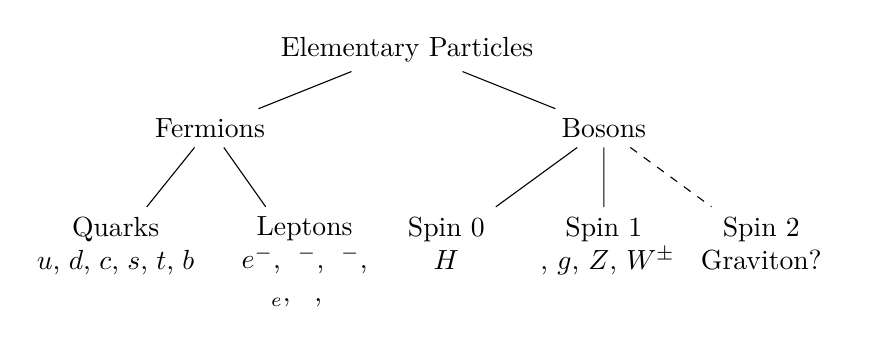
\begin{tikzpicture}[
            level 1/.style = {sibling distance = 5cm},
            level 2/.style = {sibling distance = 2cm, anchor=north}
            ]
            \node {Elementary Particles}
            child {node {Fermions}
                child {node [xshift=-0.2cm] {\parbox{2cm}{\centering Quarks\\ \Pu, \Pd, \Pc, \Ps, \Pt, \Pb}}}
                child {node [xshift=0.2cm] {\parbox{2cm}{\centering Leptons\\ \Pe, \Pmu, \Ptau, \Pnue, \Pnumu, \Pnutau}}}
            }
            child {node {Bosons}
                child {node {\parbox{2cm}{\centering Spin 0\\ \PH}}}
                child {node {\parbox{2cm}{\centering Spin 1\\ \Pphoton, \Pg, \PZ, \PWpm}}}
                child [dashed] {node {\parbox{2cm}{\centering Spin 2\\ Graviton?}}}
            };
        \end{tikzpicture}
        \caption{All of the particles in the standard model. The graviton is hypothesised but has not been observed.}
    \end{figure}
    
    \subsection{Antiparticles}
    Every particle has a corresponding \defineindex{antiparticle}, although some particles are their own antiparticles, such as the photon, Higgs boson, and \PZ{} boson.
    The \PWp{} and \PWm{} are mutually each others antiparticles, and the antiparticle of a gluon is another gluon.
    The antiparticles are defined by being identical, but with opposite charges.
    By charges here we mean electric charge, colour charge, and weak isospin, which are the charges telling us how strongly the particle couples to the electromagnetic field, strong force, and weak force respectively.
    
    The naming convention is to just stick the prefix \enquote{anti} in front of the particle's name.
    The one exception to the naming convention is the electron, whose antiparticle is the \defineindex{positron}.
    Most antiparticles are denoted as the same symbol with a bar, so \APu{} is an antiup quark.
    If the symbol usually has a sign, such as \Pe, or \PWp, then the antiparticle is denoted with the opposite sign, so \APe\index{e+@\APe|see{positron}}, or \PWm.
    
    \begin{openquestion}{}{question:are neutrinos majorana fermions?}
        It is not known if the neutrinos are their own antiparticles or not.
        Fermions which are their own antiparticles are called Majorana fermions, whereas fermions which which aren't are called Dirac fermions.
    \end{openquestion}
    
    \section{Composite Particles}
    As well as the fundamental particles, of which there are 18 particles, there are \emph{a lot} of \define{composite particles}\index{composite particle}, particles formed by combining quarks and/or antiquarks into a bound state.
    Note that there aren't composite leptons because the strong force is required to form bound states.
    
    We call a composite particle formed from quarks a \defineindex{hadron}.
    The hadrons split two types, first \define{baryons}\index{baryon}, which are formed of three quarks\footnote{here \Pq{} denotes an arbitrary quark, in particular there is no requirement that all three quarks in a baryon are the same, even if we call all three \Pq.}, \Pq\Pq\Pq, and \define{antibaryons}\index{antibaryon}, which are formed of three antiquarks, \APq\APq\APq.
    The other class is \define{mesons}\index{meson}, which are quark-antiquark pairs, \Pq\APq.
    
    The antiparticle of a composite particle has its quarks replaced with the equivalent antiquarks, and antiquarks replaced with the equivalent quarks.
    For example, the \defineindex{negative pion}, \Ppim\index{\Ppim|see{negative pion}}, is a meson with quark content \Pd\APu, and its antiparticle is the \defineindex{positive pion}, \Ppip\index{\Ppip|see{positive pion}}, another meson with quark content \Pu\APd.
    
    As well as the hadrons and mesons there have been other composite particles observed recently, although these aren't on the course as they aren't well understood yet.
    We've seen \defineindex{tetraquarks}, formed from two quarks and two antiquarks, \Pq\Pq\APq\APq, and pentaquarks, formed from four quarks and an antiquark, \Pq\Pq\Pq\Pq\APq.
    It is possible that these states aren't really new particles, but instead are \enquote{molecules} of either pairs of mesons in the tetraquark case or a hadron and a meson in the pentaquark case.
    The difference being that in the \enquote{molecules} not all quarks would be equally bound to each other, whereas if they truly are composite particles there will be no difference in how bound any pair is, apart from, for example, differences due to differing electric charges.
    
    \chapter{Feynman Diagrams}
    \define{Feynman diagrams}\index{Feynman diagram} are a way of depicting interactions between particles.
    They also correspond to the amplitude for that interaction occurring in that way.
    Each piece of the diagram can be converted into a term in some expression for the amplitude.
    More abstractly we can view Feynman diagrams as terms in a series expansion of some amplitude.
    
    When reading Feynman diagrams in this course we follow the convention that time increases to the right.
    
    \section{Currents}
    The most basic part of a Feynman diagram is a \enquote{current}.
    This is a line representing the movement of a particle through spacetime.
    The phrase current comes from electrons, where an electron moving through space is interpreted as a current.
    
    The way we depict a current depends on the type of particle.
    Fermions are depicted as a straight line with an arrow, so a fermion current looks like
    \begin{equation}
        \tikzsetnextfilename{fd-fermion-current}
        \feynmandiagram [horizontal=i to o] {
            i -- [fermion] o
        };
    \end{equation}
    Antifermions are then depicted as fermions travelling back in time, so an antifermion current looks like
    \begin{equation}
        \tikzsetnextfilename{fd-antifermion-current}
        \feynmandiagram [horizontal=i to o] {
            i -- [anti fermion] o
        };
    \end{equation}
    Spin 1 bosons, apart from gluons, so photons, \PZ{} bosons, and \PWpm{} bosons, are depicted with a wavy line:
    \begin{equation}
        \tikzsetnextfilename{fd-boson-current}
        \feynmandiagram [horizontal=i to o] {
            i -- [boson] o
        };
    \end{equation}
    Gluons are depicted with a curly line,
    \begin{equation}
        \tikzsetnextfilename{fd-gluon-current}
        \feynmandiagram [horizontal=i to o] {
            i -- [gluon] o
        };
    \end{equation}
    The Higgs boson is depicted with a dashed line,
    \begin{equation}
        \tikzsetnextfilename{fd-higgs-current}
        \feynmandiagram [horizontal=i to o] {
            i -- [scalar] o
        };
    \end{equation}
    
    It's fine not to draw an arrow for bosons as either the particle is its own antiparticle, in which case the direction does not matter, or in the case of the \PWpm{} bosons or gluons the antiparticle is of the same type, so changing direction corresponds to changing the charge (electric charge for \PWpm, and colour charge for gluons).
    
    \section{Vertex}
    The building block of any Feynman diagram is the \defineindex{vertex}, this is where currents come together.
    The exact rules for which currents can form a vertex depends on the theory in question.
    A vertex is not, by itself, a valid process.
    Instead, a diagram is a combination of vertices, connected in such a way that all conservation laws are obeyed.
    
    For now we focus on vertices involving a fermion.
    These will always have exactly two fermion currents and a boson current, so for example,
    \begin{equation}
        \tikzsetnextfilename{fd-vertex}
        \feynmandiagram [horizontal=i to v, inline=(i)] {
            i -- [fermion] v,
            v -- [boson] o1,
            v -- [fermion] o2
        };
    \end{equation}
    
    If we want to specify particular particles we can do so by labelling the lines:
    \begin{equation}
        \tikzsetnextfilename{fd-vertex-muon-photon}
        \feynmandiagram [horizontal=i to v, inline=(i)] {
            i [particle=\Pmu] -- [fermion] v,
            v -- [boson] o1 [particle=\Pphoton],
            v -- [fermion] o2 [particle=\Pmu]
        };
        \qqand
        \tikzsetnextfilename{fd-vertex-strange-gluon}
        \feynmandiagram [horizontal=i to v, inline=(i)] {
            i [particle=\Ps] -- [fermion] v,
            v -- [gluon] o1 [particle=\Pg],
            v -- [fermion] o2 [particle=\Ps]
        };
    \end{equation}
    These represent the processes \(\Pmu \to \Pmu\Pphoton\) and \(\Ps \to \Ps\Pg\).
    
    At every vertex there are conservation laws we have to apply.
    Again, the details depend on exactly what the fermions and bosons are.
    We must always conserve energy, momentum, and charge.
    There are also other quantities that must be conserved, such as muon lepton number, which is the number of muons and muon neutrinos minus the number of antimuons and antimuon neutrinos.
    We must also conserve the quark number, which is the number of quarks minus the number of antiquarks.
    
    Energy and momentum conservation can be combined into conservation of four-momentum, where
    \begin{equation}
        p^\mu = (E/c, \vv{p})
    \end{equation}
    is the four-momentum of a particle with energy \(E\) and momentum \(\vv{p}\).
    
    Given a valid vertex if we rotate it we will get another valid vertex.
    For example, rotating the \(\Ps \to \Ps\Pg\) vertex above we get the vertices
    \begin{equation}
        \tikzsetnextfilename{fd-vertex-strange-gluon-rotated-1}
        \feynmandiagram [horizontal=i to v, inline=(v)] {
            i [particle=\Pg] -- [gluon] v,
            v -- [fermion] o1 [particle=\Ps],
            v -- [anti fermion] o2 [particle=\APs]
        };
        \qqand
        \tikzsetnextfilename{fd-vertex-strange-gluon-rotated-2}
        \feynmandiagram [horizontal=v to o, inline=(v)] {
            i1 [particle=\Ps] -- [fermion] v,
            i2 [particle=\APs] -- [anti fermion] v,
            v -- [gluon] o [particle=\Pg] 
        };
    \end{equation}
    The only thing that changes here is the interpretation, these processes now represent \(\Pg \to \Ps\APs\) and \(\Ps\APs \to \Pg\).
    
    \subsection{Forces}
    \subsubsection{Electromagnetic Vertex}
    An electromagnetic vertex has a photon and any charged fermion.
    If the fermion has charge \(Q\) then the coupling constant, which we'll see later relates to how strong the interaction is, is \(Q\).
    There will be no fermion flavour change.
    \begin{equation}
        \tikzsetnextfilename{fd-vertex-electromagnetic-vertex}
        \begin{tikzpicture}[baseline=(i)]
            \begin{feynman}[horizontal=i to v, inline=(i)]
                \diagram[small]{
                    i -- [fermion] v,
                    v -- [boson] o1 [particle=\Pphoton],
                    v -- [fermion] o2,
                };
                \node [right] at (v) {\(Q\)};
            \end{feynman}
        \end{tikzpicture}
    \end{equation}
    
    \subsubsection{Strong Vertex}
    A strong vertex has a gluon and a quark.
    The coupling constant is \(\strongCoupling\).
    There will be no quark flavour change.
    \begin{equation}
        \tikzsetnextfilename{fd-vertex-strong-vertex}
        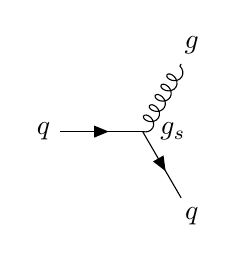
\begin{tikzpicture}[baseline=(i)]
            \begin{feynman}[horizontal=i to v, inline=(i)]
                \diagram[small]{
                    i [particle=\Pq] -- [fermion] v,
                    v -- [gluon] o1 [particle=\Pg],
                    v -- [fermion] o2 [particle=\Pq],
                };
                \node [right, xshift=0.1cm] at (v) {\(\strongCoupling\)};
            \end{feynman}
        \end{tikzpicture}
    \end{equation}
    
    \subsubsection{Neutral Current Weak Vertex}
    A neutral current weak vertex has a \PZ{} boson and any fermion.
    The coupling constant is \(\zCoupling\).
    There will be no fermion flavour change.
    \begin{equation}
        \tikzsetnextfilename{fd-vertex-weak-neutral-vertex}
        \begin{tikzpicture}[baseline=(i)]
            \begin{feynman}[horizontal=i to v, inline=(i)]
                \diagram[small]{
                    i -- [fermion] v,
                    v -- [boson] o1 [particle=\PZ],
                    v -- [fermion] o2,
                };
                \node [right] at (v) {\(\zCoupling\)};
            \end{feynman}
        \end{tikzpicture}
    \end{equation}
    
    \subsubsection{Charged Current Weak Vertex}
    A charged current weak vertex has a \PWpm{} boson and any fermion.
    The coupling constant is \(\wCoupling\).
    There will always be a fermion flavour change since it is required for charge conservation.
    \begin{equation}
        \tikzsetnextfilename{fd-vertex-weak-charged-vertex}
        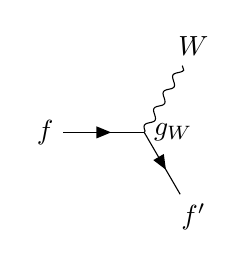
\begin{tikzpicture}[baseline=(i)]
            \begin{feynman}[horizontal=i to v]
                \diagram[small]{
                    i [particle=\(\Pf\)] -- [fermion] v,
                    v -- [boson] o1 [particle=\PW],
                    v -- [fermion] o2 [particle=\(\Pf'\)],
                };
                \node [right] at (v) {\(g_{\PW}\)};
            \end{feynman}
        \end{tikzpicture}
    \end{equation}
    
    \subsubsection{Higgs}
    A Higgs vertex has a Higgs boson and any fermion, except, at least for the purposes of this course, neutrinos.
    If the fermion has mass \(m_{\Pf}\) then the coupling constant is \(m_{\Pf}/v\), where \(v\) is a constant of value \(v \approx \qty{246}{\giga\electronvolt}\).
    There will be no fermion flavour change.
    \begin{equation}
        \tikzsetnextfilename{fd-vertex-higgs}
        \begin{tikzpicture}[baseline=(i)]
            \begin{feynman}[horizontal=i to v]
                \diagram[small]{
                    i -- [fermion] v,
                    v -- [scalar] o1,
                    v -- [fermion] o2,
                };
                \node [right] at (v) {\(m_{\Pf}/v\)};
            \end{feynman}
        \end{tikzpicture}
    \end{equation}
    
    \begin{openquestion}{}{}
        It is not known whether neutrinos couple to the Higgs field, or get their mass through another mechanism.
        Since neutrino masses are incredibly small no coupling has ever been observed, but cannot be ruled out.
    \end{openquestion}
    
    \subsection{Coupling Constants}
    The coupling constants come with related quantities, which are also referred to as the coupling constants, given by
    \begin{equation}
        \alpha = \frac{g^2}{4\pi},
    \end{equation}
    where \(g\) is the relevant coupling constant:
    \begin{itemize}
        \item \(g_{\EM} = e\) for an electromagnetic vertex, where \(e\) is the charge of the fermion involved in the interaction, not the charge of an electron;
        \item \(\strongCoupling\) for a strong vertex;
        \item \(\zCoupling\) for a neutral current weak vertex; and
        \item \(\wCoupling\) for a charged current weak vertex.
    \end{itemize}
    
    The value of \(\alpha\) is a measure of how likely a particular vertex is to occur.
    The strong force is, unsurprisingly, the strongest by which we mean that, assuming it's an allowed interaction, a strong vertex is more likely to occur than any other sort.
    This is expressed through the (relatively) high value of \(\alpha\) for the strong force:
    \begin{equation}
        \alpha_{\strongForce} \sim 1,
    \end{equation}
    as an order of magnitude estimate.
    This causes problems when we try to do perturbation theory with the strong force, as it means very often things don't converge.
    
    Next up in the list is the weak force, which has
    \begin{equation}
        \alpha_{\PW} \approx \alpha_{\PZ} \sim \frac{1}{40}.
    \end{equation}
    Last, is electromagnetism, with
    \begin{equation}
        \alpha_{\EM} = \alpha \approx \frac{1}{137}.
    \end{equation}
    
    The actual likelihood of any particular interaction depends on much more than the value of the coupling constant.
    In reality we have to consider all possible ways the interaction can occur, compute the sum of the amplitudes for these processes, and square it to get a probability.
    This means that things like the small range of the strong and weak interactions means that they are actually far less relevant on a human scale than electromagnetism and gravity.
    However, on the scale of fundamental particles, and small composite particles, the strong and weak interactions cannot be ignored.
    
    Notice that we aren't giving precise values for the coupling constants.
    This is because, despite the name, these aren't really constants.
    Instead their values depend on the energy scale at which the interaction occurs.
    This is called running of the coupling constant, and we'll see more detail later.
    
    \subsection{Boson Vertices}
    As well as vertices involving a fermion we can vertices with bosons.
    These are more varied, and we'll meet examples throughout the course.
    For now, a few examples of valid boson vertices are shown in \cref{fig:boson verticies}.
    
    \begin{figure}[p]
        \tikzsetnextfilename{fd-boson-vertex-1}
        \subcaptionbox{Two \PW{} bosons and a \PZ{} boson or a photon.}[0.31\textwidth]{
            \feynmandiagram [inline=(i)] {
                i -- [boson] v,
                v -- [boson] o1,
                v -- [boson] o2
            };
        }
        \tikzsetnextfilename{fd-boson-vertex-2}
        \subcaptionbox{Either two \PW{} bosons or two \PZ{} bosons and a Higgs boson.}[0.31\textwidth]{
            \feynmandiagram [inline=(i)] {
                i -- [boson] v,
                v -- [boson] o1,
                v -- [scalar] o2
            };
        }
        \tikzsetnextfilename{fd-boson-vertex-3}
        \subcaptionbox{Three Higgs bosons.}[0.31\textwidth]{
            \feynmandiagram [inline=(i)] {
                i -- [scalar] v,
                v -- [scalar] o1,
                v -- [scalar] o2
            };
        }
        \tikzsetnextfilename{fd-boson-vertex-4}
        \subcaptionbox{Two \PW{} bosons and either two \PW{} bosons, two \PZ{} bosons, a \PZ{} boson and a photon, or two photons.}[0.31\textwidth]{
            \feynmandiagram [inline=(v)] {
                i1 -- [boson] v,
                i2 -- [boson] v,
                v -- [boson] o1,
                v -- [boson] o2,
            };
        }
        \tikzsetnextfilename{fd-boson-vertex-5}
        \subcaptionbox{Four Higgs bosons.}[0.31\textwidth]{
            \feynmandiagram [inline=(v)] {
                i1 -- [scalar] v,
                i2 -- [scalar] v,
                v -- [scalar] o1,
                v -- [scalar] o2,
            };
        }
        \tikzsetnextfilename{fd-boson-vertex-6}
        \subcaptionbox{Two \PW{} bosons or two \PZ{} bosons and two Higgs bosons.}[0.31\textwidth]{
            \feynmandiagram [inline=(v)] {
                i1 -- [boson] v,
                i2 -- [boson] v,
                v -- [scalar] o1,
                v -- [scalar] o2,
            };
        }
        \tikzsetnextfilename{fd-boson-vertex-7}
        \subcaptionbox{Three gluons.}[0.31\textwidth]{
            \feynmandiagram [inline=(i)] {
                i -- [gluon] v,
                v -- [gluon] o1,
                v -- [gluon] o2
            };
        }
        \tikzsetnextfilename{fd-boson-vertex-8}
        \subcaptionbox{Four gluons.}[0.31\textwidth]{
            \feynmandiagram [inline=(v)] {
                i1 -- [gluon] v,
                i2 -- [gluon] v,
                v -- [gluon] o1,
                v -- [gluon] o2,
            };
        }
        \caption{Some allowed boson vertices.}
        \label{fig:boson verticies}
    \end{figure}
    
    \section{Feynman Diagrams}
    A complete Feynman diagram is then a combination of two or more vertices such that all conservation laws are obeyed.
    Exactly what the conservation laws are we'll get to later, but the basic conserved properties are charge, lepton number, quark number, and of course momentum and energy.
    
    We can consider three broad classes of interactions, first, we have \defineindex{scattering}, where two particles come in, interact, then go their separate ways.
    A simple scattering diagram is
    \begin{equation}
        \tikzsetnextfilename{fd-scattering}
        \feynmandiagram [inline=(v1), vertical=v1 to v2] {
            i1 -- [fermion] v1,
            i2 -- [fermion] v2,
            v1 -- [boson] v2,
            v1 -- [fermion] o1,
            v2 -- [fermion] o2
        };
    \end{equation}
    
    Another possibility is \defineindex{annihilation}, where two particles come in, annihilate into a boson, and then the boson produced decays into another two particles.
    A simple annihilation diagram is
    \begin{equation}
        \tikzsetnextfilename{fd-annihilation}
        \feynmandiagram [inline=(v1), horizontal=v1 to v2] {
            i1 -- [fermion] v1,
            i2 -- [fermion] v2,
            v1 -- [boson] v2,
            v1 -- [fermion] o1,
            v2 -- [fermion] o2
        };
    \end{equation}
    
    The third possibility is \defineindex{decay}, where a single particle comes in, decays into a fermion and a boson, and the boson then decays into another two fermions.
    A simple decay diagram is
    \begin{equation}
        \tikzsetnextfilename{fd-decay}
        \feynmandiagram [inline=(v1), horizontal=i to v1, layered layout] {
            i -- [fermion] v1,
            v1 -- [fermion] o1,
            v1 -- [boson] v2,
            v2 -- [fermion] o2,
            v2 -- [anti fermion] o3
        };
    \end{equation}
    
    It is important to note that Feynman diagrams are \emph{not} physical.
    We set up an experiment with some ingoing particles, and measure the outgoing particles.
    What happens between is a black box process.
    The actual process should be viewed more like the diagram
    \begin{equation}
        \rotatebox{45}{
            \feynmandiagram [inline=(v)] {
                i1 -- [fermion] v [blob] -- [fermion] o1,
                i2 -- [fermion] v -- [fermion] o2
            };
        }
    \end{equation}
    where the blob in the middle is all possible intermediate processes, all occurring at once.
    After all, from the perspective of quantum field theory a Feynman diagram is just a single term in an infinite expansion summing over all possible processes.
    
    \chapter{What do we Measure}
    \section{Types of Interactions}
    There are three different things that can occur and we can measure to get information about the particles and forces involved.
    The first is particles can decay.
    That is, we start with some particle, \(A\), and end up with particles \(1, 2, \dotsc, n\),
    \begin{equation}
        A \to 1 + 2 + \dotsb + n.
    \end{equation}
    We measure the decay rate, that is the rate at which a given decay from one particle into some other set of other particles, occurs, and compare this to theoretical predictions.
    Often we compare ratios of decay rates to get rid of constant factors and make comparison easier.
    
    The second thing that can occur is scattering.
    Here two particles, say \(A\) and \(B\), interact and produce particles \(1, 2, \dotsc, n\),
    \begin{equation}
        A + B \to 1 + 2 + \dotsb + n.
    \end{equation}
    Note that its possible that particles \(1, 2, \dotsc, n\) contain particles that are the same as the incoming particles, \(A\) and \(B\).
    However, we shouldn't think of these as the same particles, since from a quantum field theory perspective all scattering occurs by annihilating all particles, and then creating new particles.
    That said, one of the most common scattering occurrences is \(A + B \to A + B\), which is essentially the two particles bouncing off each other.
    
    The third thing that can occur is bound states, such as \defineindex{positronium} (\(\Pe\APe\)), \defineindex{charmonium} (\(\Pc\APc\)), or \defineindex{bottomonium} (\(\Pb\APb\)).
    Measuring the properties of these, such as their lifetimes, can also tell us a lot about the particles and the forces binding them.
    
    More generally we measure the transition rate for the system to go from an initial quantum state to some other final quantum state.
    
    \section{Feynman Diagrams vs.\texorpdfstring{\@}{} the Lab Picture}
    Suppose we are doing a scattering experiment scattering electrons off quarks, the quarks in term being wrapped up in a proton, since we can't get unbound quarks.
    Consider a particular scattering event in which no new particles are produced, so \(\Pe\Pq \to \Pe\Pq\).
    A Feynman diagram for this is
    \begin{equation}
        \tikzsetnextfilename{fd-feynman-diagram-picture}
        \feynmandiagram [inline=(v1), vertical=v1 to v2] {
            i1 [particle=1 \Pe] -- [fermion] v1,
            i2 [particle=2 \Pq]-- [fermion] v2,
            v1 -- [boson] v2,
            v1 -- [fermion] o1 [particle=\Pe{} 3],
            v2 -- [fermion] o2 [particle=\Pq{} 4],
        };
    \end{equation}
    Here we label the particles, with 1 and 2 being the incoming particles, and 3 and 4 being the outgoing particles.
    
    The scattering experiment could be of two types, either two beams, or a fixed target.
    However these are really the same but related by a change of frame.
    So, for simplicity, we assume two beams.
    We also assume that, like most real scattering experiments, the two beams are head on.
    Then the interaction looks something like this:
    \begin{equation}
        \tikzsetnextfilename{scattering-beams}
        \begin{tikzpicture}[baseline=(current bounding box)]
                \draw[highlight, very thick, text=black] (-3, 0) node [left] {1} .. controls (0, 0) .. (3, 2) node [above right] {3};
                \draw[highlight, very thick, text=black] (3, 0) node [right] {2} .. controls (0, 0) .. (-3, -2) node [below left] {4};
        \end{tikzpicture}
    \end{equation}
    Here the labels 1 and 2 refer to the incoming electron and quark, and the labels 3 and 4 are the outgoing electron and quark.
    
    Momentum is conserved in this interaction.
    This is a relativistic statement, so we mean that the four-momentum is conserved.
    Let \(p_1\) be the four-momentum of the incoming electron, \(p_2\) the four-momentum of the incoming quark, \(p_3\) the four-momentum of the outgoing electron, and \(p_4\) the four momentum of the outgoing quark.
    Then we have
    \begin{equation}
        p_1 + p_2 = p_3 + p_4.
    \end{equation}
    
    We will generally be interested in measuring/predicting the rate of the process, say \(1 + 2 \to 3 + 4\), that is, of all scatterings with particles \(1\) and \(2\) incoming with four-momenta \(p_1\) and \(p_2\) how many result in particles 3 and 4 with four-momenta \(p_3\) and \(p_4\).
    
    In this experiment the initial state is something that we control, we choose the particles to scatter and set their momenta based on how we create the beams.
    The final state is then what we measure.
    
    \section{Mandelstam Variables}
    Consider the following three processes:
    \begin{equation}
        \tikzsetnextfilename{fd-mandelstam-s-channel}
        \feynmandiagram[small, horizontal=v1 to v2, baseline=(current bounding box)]{
            i1 [particle=2] -- [fermion] v1,
            i2 [particle=1] -- [anti fermion] v1,
            v1 -- [boson] v2,
            v2 -- [anti fermion] o1 [particle=3],
            v2 -- [fermion] o2 [particle=4]
        };
        \qquad
        \tikzsetnextfilename{fd-mandelstam-t-channel}
        \feynmandiagram[small, vertical=v1 to v2, baseline=(current bounding box)]{
            i1 [particle=1] -- [fermion] v1,
            i2 [particle=3] -- [anti fermion] v1,
            v1 -- [boson] v2,
            v2 -- [anti fermion] o1 [particle=2],
            v2 -- [fermion] o2 [particle=4]
        };
        \qquad
        \tikzsetnextfilename{fd-mandelstam-u-channel}
        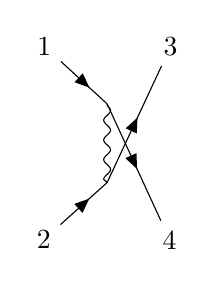
\begin{tikzpicture}[baseline=(current bounding box)]
            \begin{feynman}
                \diagram [vertical=a to b, small] {
                    i1 [particle=1] -- [fermion] a -- [draw=none] f1 [particle=3],
                    a -- [boson] b,
                    i2 [particle=2] -- [fermion] b -- [draw=none] f2 [particle=4],
                };
                \diagram* [small] {
                    (a) -- [fermion] (f2),
                    (b) -- [fermion] (f1),
                };
            \end{feynman}
        \end{tikzpicture}
    \end{equation}
    These are called the \define{\(\symbf{s}\)-channel}\index{s-channel@\(s\)-channel}, \define{\(\symbf{t}\)-channel}\index{t-channel@\(t\)-channel}, and \define{\(\symbf{u}\)-channel}\index{u-channel@\(u\)-channel} processes.
    For each one we can define a Lorentz invariant from the four momenta of the particles:
    \begin{equation}
        s \coloneqq (p_1 + p_2)^2, \qquad t \coloneqq (p_1 - p_3)^2, \qqand u \coloneqq (p_1 - p_4)^2.
    \end{equation}
    These are called the \defineindex{Mandelstam variables}
    
    The most useful of these quantities is \(s\).
    Expanding it out we get
    \begin{equation}
        s = p_1^2 + p_2^2 + 2 p_1 \cdot p_2.
    \end{equation}
    Now, if we work in the rest frame of a particle with mass \(m\) its four momentum is simply \(p = (E, \vv{0})\), and \(E^2 = m^2 + \vv{0}^2\), so \(E = m\).
    Hence \(p = (m, \vv{0})\) and so \(p^2 = m^2\).
    This is true in the rest frame, but \(p^2\) is Lorentz invariant so it must be true in any frame.
    Thus, we have
    \begin{equation}
        s = m_1^2 + m_2^2 + 2p_1 \cdot p_2,
    \end{equation}
    where \(m_1\) and \(m_2\) are the masses of particles 1 and 2.
    
    In the lab frame the four-momentum of each particle is \(p = (E, \vv{p})\), where \(E\) is the energy and \(\vv{p}\) the three-momentum.
    In our set up the two beams are head on, so the angle between the incoming particles is \ang{180}.
    This is one of the reasons \(s\) is more useful than \(t\) or \(v\), these involve \(p_3\) or \(p_4\), and we can't control the direction of the outgoing particles.
    Using this we have
    \begin{equation}
        p_1 \cdot p_2 = E_1E_2 - \vv{p_1}\cdot \vv{p_2} = E_1E_2 - \abs{\vv{p_1}}\abs{\vv{p_2}}\sin(\ang{180}) = E_1E_2 + \abs{\vv{p_1}}\abs{\vv{p_2}}.
    \end{equation}
    
    Now, we know that \(E^2 = m^2 + \abs{\vv{p}}^2\).
    Suppose we have very energetic particles, so that \(m \ll \abs{\vv{p}}\), then \(E \approx \abs{\vv{p}}\).
    Hence, we have
    \begin{equation}
        p_1 \cdot p_2 = E_1E_2 + \abs{\vv{p_1}}\abs{\vv{p_2}} \approx E_1 E_2 + E_1E_2 = 2E_1E_2.
    \end{equation}
    Further, assuming that \(m_1 \ll E_1\) and \(m_2 \ll E_2\) we have
    \begin{equation}
        s = m_1^2 + m_2^2 + 2p_1 \cdot p_2 \approx m_1^2 + m_2^2 + 4E_1E_2 \approx 4E_1E_2.
    \end{equation}
    
    If both beams have the same energy, \(E\), then \(s = 4E^2\), and so \(\sqrt{s} = 2E\), which is the total energy of the two particles scattering.
    This means that \(\sqrt{s}\) has a nice interpretation as the energy of the collision.
    
    \section{Fermi's Golden Rule}
    We are interested in the transition rate for going from some state \(\ket{i}\) to some state \(\ket{f}\).
    We suppose that the system evolves under the Hamiltonian
    \begin{equation}
        \operator{H} = \operator{H}_0 + \operator{H}'(x),
    \end{equation}
    where \(\operator{H}_0\) is a time independent Hamiltonian for which we can solve the Schrödinger equation and \(\operator{H}'(x)\) is the interaction Hamiltonian, which induces the transitions between states.
    The interaction is generally position dependent.
    The state of the system then evolves according to the Schrödinger equation:
    \begin{equation}
        i \diffp{}{t}\ket{\psi, t} = \operator{H}\ket{\psi, t} = [\operator{H}_0 + \operator{H}'(x)]\ket{\psi, t}.
    \end{equation}
    
    Fermi's golden rule says that the transition rate from state \(\ket{i}\) to state \(\ket{f}\) is given by
    \begin{equation}
        \Gamma_{fi} = 2\pi \abs{T_{fi}}^2 \rho(E_i)
    \end{equation}
    where \(\Gamma_{fi}\) is the transition rate, \(T_{fi}\) is the transition matrix, and \(\rho(E_i)\) is the density of accessible states.
    The full derivation is in \cref{app:fermi's golden rule}.
    
    To first order the transition matrix is simply the matrix elements of the perturbation Hamiltonian,
    \begin{equation}
        T_{fi} = \bra{f} \operator{H}' \ket{i}.
    \end{equation}
    This represents a process where the state evolves directly from \(\ket{i}\) to \(\ket{f}\).
    To second order the transition matrix is
    \begin{equation}
        T_{fi} = \bra{f} \operator{H}' \ket{i} + \sum_{k \ne i} \frac{\bra{f} \operator{H}' \ket{k} \bra{k} \operator{H}' \ket{i}}{E_i - E_k}.
    \end{equation}
    The second term accounts for all transitions via an intermediate state, \(\ket{k}\).
    Continuing on the next term would have transitions via two intermediate states and so on.
    
    \subsection{Density of States}
    We want our processes to be physical.
    This means they have to obey several conservation laws, such as energy and momentum conservation.
    We enforce this by having a Dirac delta in our terms, such as
    \begin{equation}
        \delta(E_i - E_f), \qquad \delta^3(\vv{p_i} - \vv{p_f}), \qqand \delta^4(p_i - p_f),
    \end{equation}
    where \(E_i\) and \(E_f\) are the total energy of the initial and final states, \(\vv{p_i}\) and \(\vv{p_f}\) are the total three-momenta of the initial and final states, and \(p_i\) and \(p_f\) are the total four-momenta of the initial and final states.
    
    The density of final accessible states depends on the kinematics of the process being considered.
    In particular, the initial energy, \(E_i\), is the total amount of energy available to the final states.
    The density of states is given by integrating over all states with energy conservation enforced by a Dirac delta:
    \begin{equation}
        \rho(E_i) = \int \delta(E_i - E) \dd{n} = \int \delta(E_i - E) \diff{n}{E} \dd{E} = \diff{n}{E}[E = E_i].
    \end{equation}
    Here \(\dl{n}\) gives the number of states with energies between \(E\) and \(E + \dl{E}\).
    
    Fermi's golden rule is then that
    \begin{equation}
        \Gamma_{fi} = 2\pi \int \abs{T_{fi}}^2 \delta(E_i - E) \dd{n}.
    \end{equation}
    
    The complication with this is that states are quantised, so this integral is nontrivial.
    A spinless, massless particle can be described with a plane wave
    \begin{equation}
        \psi = A\e^{-ip\cdot x}.
    \end{equation}
    We consider the particle to be in a box of side length \(a\) and impose vanishing boundary conditions.
    Normalising the wave function gives us \(A = 1/V\) where \(V = a^3\) is the volume of the box.
    The momentum of the particle is then quantised as
    \begin{equation}
        p_i = \frac{2\pi n_i}{a}.
    \end{equation}
    
    The volume occupied by a state in momentum space is then
    \begin{equation}
        \dl{^3\vv{p}} = \dl{p_x} \dd{p_y}\dd{p_z} = \left( \frac{2\pi}{a} \right)^3 = \frac{(2\pi)^3}{V}.
    \end{equation}
    The number of states, \(\dl{n}\), with a momentum in the range \(p\) to \(\dl{p}\) is the volume in momentum space of the spherical shell of inner radius \(p\) and thickness \(\dl{p}\) divided by the volume of a single state:
    \begin{equation}
        \dl{n} = 4\pi p^2 \dd{p} \frac{V}{(2\pi)^3}.
    \end{equation}
    We can choose our box such that we have one particle per unit volume, and call this volume 1, we then have
    \begin{equation}
        \dl{n} = \frac{4p^2 \dd{p}}{(2\pi)^3} = \frac{\dl{^3\vv{p}}}{(2\pi)^3}.
    \end{equation}
    
    For example, consider a decay \(A \to 1 + 2 + \dotsb + N\).
    Then
    \begin{equation}
        \dl{n} = (2\pi)^3 \prod_{i=1}^{N} \frac{\dl{^3\vv{p_i}}}{(2\pi)^3} \delta^3\left( \vv{p_A} - \sum_{i = 1}^{N} \vv{p_i} \right).
    \end{equation}
    
    So far we haven't considered the effects of relativity.
    Our box of unit volume will be Lorentz contracted in the direction of motion.
    The contraction is proportional to \(\gamma\), which for a single particle of mass \(m\) and energy \(E\) is given by \(\gamma = E/m\).
    The fix is to redefine the wave function to \(\psi'\), so that
    \begin{equation}
        \int \psi'^*\psi' \dd{V} \propto E.
    \end{equation}
    The convention is to choose the constant of proportionality to be 2, and then set \(\psi' = \sqrt{2E}\psi\).
    We can then define a Lorentz invariant matrix element:
    \begin{equation}
        \amplitude_{fi} = \sqrt{2E_1 \cdot 2E_2 \dotsm 2E_N} T_{fi}
    \end{equation}
    where the product is over the energies of all particles, in both the initial and final states.
    
    The transition rate is then
    \begin{equation}
        \Gamma_{fi} = 2\pi \int \abs{T_{fi}}^2 \delta(E_i - E) \dd{n}.
    \end{equation}
    For simplicity consider the decay \(A \to 1 + 2\), the transition rate is
    \begin{equation}
        \Gamma_{fi} = 2\pi \int \abs{T_{fi}}^2 \delta(E_A - E_1 - E_2) \dd{n}.
    \end{equation}
    Moving to momentum space we have
    \begin{equation}
        \dl{n} = (2\pi)^3 \frac{\dl{^3\vv{p_1}}}{(2\pi)^3} \frac{\dl{^3\vv{p_2}}}{(2\pi)^3} \delta^3(\vv{p_A} - \vv{p_1} - \vv{p_2}).
    \end{equation}
    Making this Lorentz invariant we have
    \begin{equation}
        \amplitude_{fi} = \sqrt{2E_12E_22E_A} T_{fi} \implies T_{fi} = \frac{\amplitude_{fi}}{\sqrt{2E_12E_22E_A}}
    \end{equation}
    and so
    \begin{equation}
        \Gamma_{fi} = \frac{(2\pi)^4}{2E_A} \int \abs{\amplitude_{fi}}^2 \delta^4(p_A - p_1 - p_2) \frac{\dl{^3\vv{p_1}}}{(2\pi)^32E_1} \frac{\dl{^3\vv{p_2}}}{(2\pi)^32E_2}.
    \end{equation}
    
    This is just a rewriting of Fermi's golden rule, but now in an explicitly Lorentz invariant form.
    There are several key features:
    \begin{itemize}
        \item The Lorentz invariant phase space measure, \(\dl{^3\vv{p}}/[(2\pi)^32E]\).
        \item Energy and Momentum conservation from the Dirac delta.
        \item The decay rate is inversely proportional to the energy fo the decaying particle.
        \item The Lorentz invariant \(\amplitude_{fi}\) is the part that encodes the physics of the process, and working out what value this should have for a given interaction is the goal of a large part of quantum field theory.
    \end{itemize}
    
    Consider the \(A \to 1 + 2\) decay again, we can partially evaluate the integral and we find that
    \begin{equation}
        \Gamma_{fi} = \frac{\abs{\vv{p}^*}}{32\pi^2 m_A^2} \int \abs{\amplitude_{fi}}^2 \dd{\Omega}
    \end{equation}
    where \(\abs{\vv{p}^*}\) is the magnitude of the three-momenta of particles 1 and 2 in the rest frame of \(A\), note that they must have the same magnitude of three-momenta as the initial momentum is zero in this frame.
    The integral is over all angles, with \(\dl{\Omega} = \sin\theta \dd{\varphi} \dd{\vartheta}\).
    This is valid for all two body decays.
    
    If instead we consider scattering, \(A + B \to 1 + 2\), again in the centre of mass frame then we find that
    \begin{equation}
        \sigma = \frac{1}{64\pi^2s} \frac{\abs{\vv{p_f}^*}}{\abs{\vv{p_i}^*}} \int \abs{\amplitude_{fi}}^2 \dd{\Omega}
    \end{equation}
    where \(\abs{\vv{p_i}^*}\) and \(\abs{\vv{p_f}^*}\) are the magnitude of the three-momenta of the initial and final states in the centre of mass frame, and \(s = (p_A + p_B)^2\) is a Mandelstam variable.
    Note that this is Lorentz invariant, despite the appearance of three-vectors.
    
    \part{Fermions}    
    \chapter{Deriving the Dirac Equation}
    \section{Schrödinger}
    Start with the nonrelativistic energy-momentum relation
    \begin{equation}
        E = \frac{p^2}{2m} + V,
    \end{equation}
    where \(p\) is the magnitude of the particles momentum, \(m\) is its mass, and \(V\) is some potential.
    To get the Schrödinger equation we substitute in operators:
    \begin{equation}
        \operator{p}_j = -i\diffp{}{x^j} = -i\partial_j, \qquad \vecoperator{p} = -i\grad, \qqand E = i\diffp{}{t} = i\partial_t.
    \end{equation}
    Acting with the resulting operator on a wave function we get the \defineindex{Schrödinger equation}:
    \begin{equation}
        i\diffp{\psi}{t} = \left( -\frac{1}{2m} \laplacian + V \right)\psi.
    \end{equation}
    Note that this is first order in time, and second order in space, which makes it not relativistic.
    
    \section{Klein--Gordon Equation}
    If we want a relativistic equation we should start with the relativistic energy-momentum relation,
    \begin{equation}
        E^2 = \vv{p}^2 + m^2.
    \end{equation}
    Substituting in the same operators we get
    \begin{equation}
        \diffp[2]{\varphi}{t} = (\laplacian - m^2)\varphi \implies (\dalembertian + m^2)\varphi = 0.
    \end{equation}
    Here \(\dalembertian = \partial_\mu \partial^\mu\) is the d'Alembert operator.
    This is the \defineindex{Klein--Gordon equation}, it describes free spin 0 bosons.
    The problem is that we have negative energy solutions, and worse still, if we try to interpret \(\varphi\) as a wave function then we can get negative probabilities.
    
    \section{Dirac Equation}
    The negative energies appear due to the presence of \(E^2\), giving a positive and negative branch when we take the square root.
    To avoid this Dirac looked for a first order relationship between energy and momentum.
    He started with
    \begin{equation}
        \operator{E}\psi = (\vv{\alpha} \cdot \vecoperator{p} + \beta m)\psi
    \end{equation}
    where \(\vv{\alpha}\) and \(\beta\) are some constants.
    Inserting the operators we have
    \begin{equation}
        i\diffp{\psi}{t} = \left( -i\alpha_x \diffp{}{x} - i\alpha_y \diffp{}{y} - i\alpha_z \diffp{}{z} + \beta m \right)\psi.
    \end{equation}
    Defining \(\gamma^0 = \beta\), \(\gamma^i = \beta \alpha_i\) some rearranging gives this equation in the form
    \begin{equation}
        \left( i\gamma^0 \diffp{}{t} + i\gamma^1 \diffp{}{x} + i\gamma^2 \diffp{}{y} + i\gamma^3 \diffp{}{z} - m \right) \psi = 0.
    \end{equation}
    This can be written more compactly as
    \begin{equation}
        (i\gamma^\mu \partial_\mu - m)\psi = 0.
    \end{equation}
    Defining \(\slashed{a} \coloneqq \gamma^\mu a_\mu\)\index{\(\slashed{a} \coloneqq \gamma^\mu a_\mu\)} we can write this even more compactly as
    \begin{equation}
        (i\slashed{\partial} - m)\psi = 0.
    \end{equation}
    This is the \defineindex{Dirac equation}, it describes spin 1/2 fermions.
    
    \section{The \texorpdfstring{\(\gamma\)}{gamma} Coefficients}
    Suppose that \(\psi\) satisfies both the Dirac equation, we can then write
    \begin{equation}
        (-i\slashed{\partial} - m)(i\slashed{\partial} - m)\psi = 0.
    \end{equation}
    Expanding this we get
    \begin{equation}
        (\slashed{\partial}^2 +m^2)\psi = 0.
    \end{equation}
    This looks slightly like the Klein--Gordon equation, so suppose that \(\psi\) also satisfies this, that is
    \begin{equation}
        (\dalembertian + m^2)\psi = 0.
    \end{equation}
    Expanding the the \(\slashed{\partial} = \gamma^\mu \partial_\mu\) we get
    \begin{align}
        \slashed{\partial}^2 &= \gamma^\mu\partial_\mu \gamma^\nu\partial_\nu\\
        &= (\gamma^0)^2\partial_t^2 + (\gamma^1)^2\partial_x^2 + (\gamma^2)^2\partial_y^2 + (\gamma^3)^2\partial_z^2\\
        &+ \gamma^0\gamma^1 \partial_t\partial_x + \gamma^0\gamma^2 \partial_t\partial_y + \gamma^0\gamma^3 \partial_t\partial_z\\
        &+ \gamma^1\gamma^2 \partial_x\partial_y + \gamma^1\gamma^3 \partial_x\partial_z + \gamma^2\gamma^3 \partial_y\partial_z.
    \end{align}
    Compare this to the expanded d'Alembertian:
    \begin{equation}
        \dalembertian = \partial_t^2 - \partial_x^2 - \partial_y^2 - \partial_z^2.
    \end{equation}
    In order for \(\psi\) to satisfy both the Klein--Gordon equation and the Dirac equation we must have
    \begin{equation}
        (\gamma^0)^2 = 1, \qquad (\gamma^i)^2 = -1, \qqand \gamma^\mu \gamma^\nu = -\gamma^\nu \gamma^\mu.
    \end{equation}
    More compactly we can write these requirements as\index{\(\gamma^\mu\)}\index{gamma matrices}
    \begin{equation}
        \anticommutator{\gamma^\mu}{\gamma^\nu} = 2\eta^{\mu\nu}
    \end{equation}
    where \(\anticommutator{A}{B} \coloneqq AB + BA\) is the \defineindex{anticommutator} and \(\eta\) is the metric tensor.
    
    \itshape
    While this isn't a proof that \(\gamma^\mu\) must satisfy this we take it to be so.
    The relation
    \begin{equation}
        \anticommutator{\gamma^\mu}{\gamma^\nu} = 2\varepsilon^{\mu\nu}
    \end{equation}
    defines a Clifford algebra, \(\operatorname{Cl}_{1,3}(\reals)\), which can be thought of as the space of all linear operators from spacetime, \(V\), to itself, that is, \(\operatorname{End}(V)\).
    We can then think of \(\gamma^\mu\) as the generators of this algebra, or a representation of this algebra.
    \normalshape
    
    The lowest dimensional set of matrices satisfying the required properties\footnote{That is, the lowest dimensional nontrivial representation of \(\operatorname{Cl}_{1,3}(\reals)\).} is
    \begin{alignat}{2}
        \gamma^0 &= 
        \begin{pmatrix}
            1 & 0 & 0 & 0 \\
            0 & 1 & 0 & 0 \\
            0 & 0 & -1 & 0 \\
            0 & 0 & 0 & -1
        \end{pmatrix}
        , \qquad & \gamma^1 &= 
        \begin{pmatrix}
            0 & 0 & 0 & 1 \\
            0 & 0 & 1 & 0 \\
            0 & -1 & 0 & 0\\
            -1 & 0 & 0 & 0
        \end{pmatrix}
        ,\\
        \gamma^2 &= 
        \begin{pmatrix}
            0 & 0 & 0 & -i \\
            0 & 0 & i & 0 \\
            0 & i & 0 & 0 \\
            -i & 0 & 0 & 0
        \end{pmatrix}
        , \qquad & \gamma^3 &= 
        \begin{pmatrix}
            0 & 0 & 1 & 0 \\
            0 & 0 & 0 & -1 \\
            1 & 0 & 0 & 0\\
            0 & -1 & 0 & 0
        \end{pmatrix}
        .
    \end{alignat}
    This can be written more compactly as
    \begin{equation}
        \gamma^0 = 
        \begin{pmatrix}
            I & 0\\
            0 & -I
        \end{pmatrix}
        = \sigma^3 \otimes I, \qqand \gamma^i =
        \begin{pmatrix}
            0 & \sigma^i\\
            -\sigma^i
        \end{pmatrix}
        = i\sigma^2 \otimes \sigma^i
    \end{equation}
    where \(I\) is the 2-dimensional identity matrix and \(\sigma^i\) are the \defineindex{Pauli spin matrices}:
    \begin{equation}
        I = 
        \begin{pmatrix}
            1 & 0 \\
            0 & 1
        \end{pmatrix}
        , \quad \sigma^1 = 
        \begin{pmatrix}
            0 & 1\\
            1 & 0
        \end{pmatrix}
        , \quad \sigma^2 = 
        \begin{pmatrix}
            0 & -i\\
            i & 0
        \end{pmatrix}
        , \qand \sigma^3 = 
        \begin{pmatrix}
            1 & 0\\
            0 & -1
        \end{pmatrix}
        .
    \end{equation}
    
    \chapter{Solving the Dirac Equation}
    \section{Spinors}
    The Dirac equation,
    \begin{equation}
        (i\slashed{\partial} - m)\psi = 0,
    \end{equation}
    can be written in terms of \(4\times 4\) matrices, \(\slashed{\partial} = \gamma^\mu\partial_\mu\) and \(m\) (with an implicit factor of the \(4\times 4\) identity, \(I_4\)), acting on \(\psi\).
    This means that \(\psi\) must have four components.
    We can think of it as a \(4 \times 1\) matrix, but it is \emph{not} a four-vector\footnote{That is, it doesn't transform as a four-vector under \(\specialOrthogonal^+(1,3)\), they transform under a different representation which cannot be constructed from tensor products of the fundamental representation in the usual way.}.
    We call objects like this \define{spinors}\index{spinor}.
    
    We make the ansatz that \(\psi\) has the form
    \begin{equation}
        \psi(x) = u(p) \e^{-ip\cdot x},
    \end{equation}
    where \(u(p)\) is some spinor and \(\exp[-ip\cdot x]\) is a phase factor.
    This means that
    \begin{equation}
        \psi(x) = 
        \begin{pmatrix}
            \psi^1(x)\\ \psi^2(x)\\ \psi^3(x)\\ \psi^4(x)
        \end{pmatrix}
        =
        \begin{pmatrix}
            \varphi^1(p)\\ \varphi^2(p)\\ \varphi^3(p)\\ \varphi^4(p)
        \end{pmatrix}
        \e^{-ip\cdot x} = u(p)\e^{-ip\cdot x}.
    \end{equation}
    
    Now notice that \(i\partial_\mu\) acting on \(\e^{-ip\cdot x}\) gives \(p_\mu \e^{-ip\cdot x}\), and in particular \(\partial_\mu\) has no effect on \(u(p)\), since it has no position dependence.
    We can then write the Dirac equation as
    \begin{equation}
        (\slashed{p} - m)u(p) = 0,
    \end{equation}
    having divided through by the phase factor.
    
    We can write this in the significantly less compact form
    \begin{equation}
        \begin{pmatrix}
            E - m & 0 & -p_z & -p_x + ip_y\\
            0 & E - m & -p_x - ip_y & p_z\\
            p_z & p_x - ip_y & -E - m & 0\\
            p_x + ip_y & -p_z & 0 & -E - m
        \end{pmatrix}	
        \begin{pmatrix}
            \varphi^1(p)\\ \varphi^2(p)\\ \varphi^3(p)\\ \varphi^4(p)
        \end{pmatrix}
        = 0.
    \end{equation}
    
    To solve this move to the rest frame of the particle, so \(p_i = 0\), this then becomes
    \begin{equation}
        \begin{pmatrix}
            E - m & 0 & 0 & 0\\
            0 & E - m & 0 & 0\\
            0 & 0 & -E - m & 0\\
            0 & 0 & 0 & -E - m
        \end{pmatrix}	
        \begin{pmatrix}
            \varphi^1(p)\\ \varphi^2(p)\\ \varphi^3(p)\\ \varphi^4(p)
        \end{pmatrix}
        = 0.
    \end{equation}
    This is just an eigenvalue equation, for the matrix \(\diag(E, E, -E, -E)\), and there are four eigenspinors
    \begin{equation}
        u^1 = N
        \begin{pmatrix}
            1\\ 0\\ 0\\ 0
        \end{pmatrix}
        , \quad u^2 = N
        \begin{pmatrix}
            0\\ 1\\ 0\\ 0
        \end{pmatrix}
        , \quad u^3 = N
        \begin{pmatrix}
            0\\ 0\\ 1\\ 0
        \end{pmatrix}
        , \qand u^4 = N
        \begin{pmatrix}
            0\\ 0\\ 0\\ 1
        \end{pmatrix}
        .
    \end{equation}
    Here \(N\) is a normalisation factor, which is usually \(\sqrt{E + m}\) so \(u^\hermit u = 2E\) for all four spinors.
    The first two solutions here correspond to eigenvalues of \(E = +m\), whereas the second two correspond to eigenvalues of \(E = -m\).
    This means that despite Dirac's best attempts we \emph{still} have negative energy solutions.
    The full solution to the Dirac equation for a particle at rest is then
    \begin{equation}
        \psi^1 = N
        \begin{pmatrix}
            1\\ 0\\ 0\\ 0
        \end{pmatrix}
        \e^{-imt}, \quad u^2 = N
        \begin{pmatrix}
            0\\ 1\\ 0\\ 0
        \end{pmatrix}
        \e^{-imt}, \quad u^3 = N
        \begin{pmatrix}
            0\\ 0\\ 1\\ 0
        \end{pmatrix}
        \e^{imt}, \qand u^4 = N
        \begin{pmatrix}
            0\\ 0\\ 0\\ 1
        \end{pmatrix}
        \e^{imt}.
    \end{equation}
    We get four solutions, which is quite different to the Klein--Gordon equation.
    The reason for this is the Klein--Gordon equation represents spin 0 particles, whereas the Dirac equation represents spin \(1/2\) particles, and the four solutions correspond to four types of spin \(1/2\) particles:
    \begin{itemize}
        \item \(u^1\) corresponds to a positive energy spin up solution.
        \item \(u^2\) corresponds to a positive energy spin down solution.
        \item \(u^3\) corresponds to a negative energy spin down solution.
        \item \(u^4\) corresponds to a negative energy spin up solution.
    \end{itemize}
    
    \section{Interpreting Negative Energies}
    \subsection{Dirac Sea}
    The Dirac sea interpretation says that the vacuum state corresponds to all negative energy states being filled.
    The exclusion principle then prevents the entire system from decaying to arbitrarily large negative energies.
    What we view as a particle is then actually a particle being excited to a positive energy state from a negative energy state.
    At the same time this leaves a hole in the negative energy states, which is what we view as an antiparticle.
    
    This interpretation means that the process \(\Pphoton \to \Pe \APe\) is just an electron in a negative energy state absorbing a photon, and being excited to a positive energy state, leaving behind a hole.
    Similarly the process \(\Pe\APe\to\Pphoton\) is the electron falling back to the negative energy state, emitting a photon and filling the hole.
    
    This interpretation lead to Dirac predicting the existence of the positron before it was experimentally discovered.
    
    \subsection{Feynman--St\"uckelberg}
    The more modern interpretation is that the negative energy solutions correspond to negative energy particles propagating backwards in time, which correspond to positive energy antiparticles propagating forward in time.
    This is (part of) the reason we use arrows going backwards in time to represent antiparticles in a Feynman diagram.
    
    In this interpretation the process \(\Pe\APe \to \Pphoton\) corresponds either to an electron and positron annihilating, or to an electron with positive energy coming in, emitting a photon to have negative energy, and then leaving going backwards in time.
    
    \section{General Solution}
    It is possible to solve the Dirac equation in a general frame\footnote{see \course{Quantum Theory} or \course{Quantum Field Theory} for details}, not just the rest frame of the particle.
    The result is again four different spinors, first
    \begin{equation}
        u^1(p) = N
        \begin{pmatrix}
            1\\ 0\\
            \frac{p_z}{E + m}\\
            \frac{p_x + ip_y}{E + m}
        \end{pmatrix}
        , \qqand
        u^2(p) = N
        \begin{pmatrix}
            0\\ 1\\
            \frac{p_x - ip_y}{E + m}\\
            \frac{-p_z}{E + m}
        \end{pmatrix}
    \end{equation}
    where \(E = + \sqrt{m^2 + \vv{p}^2}\).
    Then we also have the negative energy solutions
    \begin{equation}
        u^3(p) = N
        \begin{pmatrix}
            \frac{p_z}{E - m}\\
            \frac{p_x + ip_y}{E - m}\\
            1\\ 0
        \end{pmatrix}
        , \qqand
        u^4(p) = N
        \begin{pmatrix}
            \frac{p_x - ip_y}{E - m}\\
            \frac{-p_z}{E - m}\\
            0\\ 1
        \end{pmatrix}
    \end{equation}
    where \(E = -\sqrt{m^2 + \vv{p}^2}\).
    
    To get rid of negative energy solutions we instead define explicit antiparticle spinors,
    \begin{equation}
        v^1(p) = u^4(-p), \qqand v^2(p) = u^3(-p).
    \end{equation}
    Note that \(4\) and \(1\) go together and \(2\) and \(3\) go together, which is probably not what one would expect, and corresponds to the weirdness with \(u^1\), \(u^2\), \(u^3\), and \(u^4\) representing spin up, down, down, and up solutions respectively.
    The antiparticle spinors are solutions to
    \begin{equation}
        (\slashed{p} \mathbin{\textcolor{highlight}{+}} m)v = 0.
    \end{equation}
    
    \section{Helicity}
    Recall that we have two operators measuring spin:
    \begin{equation}
        \vecoperator{S}^2\ket{\psi} = s(s + 1)\ket{\psi}, \qqand \operator{S}_z\ket{\psi} = m_s\ket{\psi}.
    \end{equation}
    Here \(\operator{S}_z\) measures the spin along the \(z\)-axis.
    Rather than measure along an arbitrarily chosen axis it is usually preferable to measure spin relative to the direction of travel of the particle.
    This can be done by defining the \defineindex{helicity}
    \begin{equation}
        \operator{h} \coloneqq \frac{\vecoperator{S} \cdot \vecoperator{p}}{\abs{\vv{p}}}.
    \end{equation}
    
    For a spin \(1/2\) particle \(m_s\) can be \(\pm 1/2\).
    Similarly \(h\), defined by \(\operator{h}\ket{\psi} = h\ket{\psi}\), can take the values\footnote{some texts define helicity with a factor of 2, so that \(h\) takes values of \(\pm 1\)} \(\pm 1/2\).
    If it takes the value \(1/2\) then the spin is aligned in the direction of travel and we say the particle is \defineindex{right handed}.
    If \(h\) takes the value \(-1/2\) then the spin is antialigned in the direction of travel and we say the particle is \defineindex{left handed}.
    
    Note that the helicity is not a Lorentz invariant, except for in the case where the particle is massless and helicity coincides with chirality.
    
    If we define the direction of the momentum by a unit vector,
    \begin{equation}
        \vh{n} = (\sin\vartheta \cos\varphi, \sin\vartheta\cos\varphi, \cos\vartheta),
    \end{equation}
    then we can work with helicity eigenstates given by
    \begin{alignat}{2}
        u_{\uparrow} &= N \left(
        \begin{array}{r}
            \cos(\vartheta/2)\\
            \e^{i\varphi}\sin(\vartheta/2)\\
            \xi\cos(\vartheta/2)\\
            \xi\e^{i\varphi}\sin(\vartheta/2)
        \end{array}
        \right), \qquad & u_{\downarrow} &= N \left(
        \begin{array}{r}
            -\sin(\vartheta/2)\\
            \e^{i\varphi}\cos(\vartheta/2)\\
            \xi\sin(\vartheta/2)\\
            -\xi\e^{i\varphi}\cos(\vartheta/2)
        \end{array}
        \right),\\
        v_{\uparrow} &= N \left(
        \begin{array}{r}
            \xi\sin(\vartheta/2)\\
            -\xi\e^{i\varphi}\cos(\vartheta/2)\\
            -\sin(\vartheta/2)\\
            \e^{i\varphi}\cos(\vartheta/2)
        \end{array}
        \right), \qquad & v_{\downarrow} &= N \left(
        \begin{array}{r}
            \xi\cos(\vartheta/2)\\
            \xi\e^{i\varphi}\sin(\vartheta/2)\\
            \cos(\vartheta/2)\\
            \e^{i\varphi}\sin(\vartheta/2)
        \end{array}
        \right),
    \end{alignat}
    where \(\xi = \abs{\vv{p}}/(E + m)\).
    
    Notice that the transformation
    \begin{equation}
        \vh{n} \mapsto (\sin(\vartheta + 2\pi)\cos\varphi, \sin(\vartheta + 2\pi), \cos(\vartheta + 2\pi))
    \end{equation}
    doesn't result in the same spinors, instead it gives us back their negatives.
    It requires a \(4\pi\) \enquote{rotation} to take the spinors back to their original value.
    
    One nice thing about these eigenstates is that for low momentum particles they become significantly simpler if we neglect the \(\abs{\vv{p}}/(E + m)\) terms.
    Many of our calculations will use these helicity eigenstates as a basis.
    
    \chapter{Getting Probabilities}
    \section{Interpreting the Spinor Wave Function}
    In nonrelativistic quantum mechanics we have a wave function, \(\psi\), which is a complex number valued function encoding all of the information we have about a quantum system.
    This wave function is the solution to the Schrödinger equation.
    We have the further restriction that \(\psi\) must be square integrable, to allow us to normalise probabilities.
    To extract this information we consider \(\rho(\vv{x}, t) \coloneqq \psi^*(t, \vv{x}) \psi(t, \vv{x}) = \abs{\psi(t, \vv{x})}^2\), which we interpret as a probability density.
    We can also define a three-vector probability current, \(\vv{j}(t, \vv{x})\)
    To do this we consider the rate of change of the total probability in some region, \(V\), of spacetime:
    \begin{equation}
        \diffp{}{t}\int_V \rho \dd{V}.
    \end{equation}
    The rate of change of the total probability is equal to the flux out through the boundary of \(V\), denoted \(\partial V\).
    This is given by 
    \begin{equation}
        \diffp{}{t} \int_V \rho \dd{V} = -\int_{\partial V} \vv{j} \cdot \dl{\vv{S}} = -\int_V \div\vv{j} \dd{V}
    \end{equation}
    where the last step is the divergence theorem.
    We then have the continuity equation
    \begin{equation}
        \diffp{\rho}{t} = -\div\vv{j} \implies \diffp{\rho}{t} + \div\vv{j} = 0.
    \end{equation}
    It is also possible to express \(\vv{j}\) in terms of the wave function:
    \begin{equation}
        \vv{j} = -\frac{i}{2m} \left( \psi^* \grad \psi - \psi \grad \psi^* \right).
    \end{equation}
    We can write this relativistically by defining \(j^\mu = (\rho, \vv{j})\) and then the continuity equation is
    \begin{equation}
        \partial_\mu j^\mu = 0.
    \end{equation}
    
    Things don't change that much when we consider spinors.
    We still have a wave function, \(\psi\), but now it's spinor valued\footnote{Formally if \(\rho \colon \operatorname{Spin}(p, q) \to \generalLinear(V)\) is a representation of the spin group, which is the double cover of \(\specialOrthogonal^+(p, q, \reals)\), which is the (proper orthochronous) Lorentz group when \(p = 1\) and \(q = 3\), then spinors are elements of \(V\).}.
    
    So, to complete our probability finding step we just need to find a way to \enquote{square} a spinor to get a probability density and a probability current.
    Appealing to the normal wave function case the obvious generalisation from the one (complex) dimensional complex-number-valued wave function to the four (in the Dirac representation) dimensional spinor-valued wave function is to replace \(\psi^*\psi\) with \(\psi^\hermit \psi\).
    If we have a four-component spinor
    \begin{equation}
        \psi = 
        \begin{pmatrix}
            \varphi^1\\ \varphi^2\\ \varphi^3\\ \varphi^4
        \end{pmatrix}
        \e^{-ip\cdot x},
    \end{equation}
    then we can define \(\psi^\hermit\) to be
    \begin{equation}
        \psi^\hermit \coloneqq 
        \begin{pmatrix}
            \varphi^{1*} & \varphi^{2*} & \varphi^{3*} & \varphi^{4*}
        \end{pmatrix}
        \e^{ip\cdot x}.
    \end{equation}
    
    Since we want to work relativistically we look directly for \(j^\mu\), rather than finding \(\rho\) and \(\vv{j}\) separately.
    To do so we need to combine our spinor with something with a Lorentz index, in order to get a four vector.
    The obvious choice when it comes to spinors is a gamma matrix, \(\gamma^\mu\).
    After some consideration we see that if we consider \(\psi^\hermit \gamma^\mu \psi\) then, for a fixed value of \(\mu\), this just gives a number, so allowing \(\mu\) to take values \(\mu = 0, 1, 2, 3\) we get a four-vector.
    
    However, there is a problem.
    This quantity is not Lorentz invariant\footnote{see \course{Quantum Field Theory} for details}.
    It turns out that a small modification fixes this, we should instead consider \(j^\mu \coloneqq \psi^\hermit \gamma^0\gamma^\mu \psi\).
    This is a four-vector with components
    \begin{equation}
        j^\mu = \psi^\hermit \gamma^0 \gamma^\mu \psi = (\psi^\hermit \psi, \psi^\hermit \gamma^0\gamma^1\psi, \psi^\hermit \gamma^0\gamma^2\psi, \psi^\hermit \gamma^0\gamma^3\psi),
    \end{equation}
    where we've used \((\gamma^0)^2 = 1\).
    Quantities of the form \(a^\hermit \gamma^0\) are common enough that we define \(\overbar{a} \coloneqq a^\hermit \gamma^0\)\index{\(\overbar{\psi} \coloneqq a^\hermit\gamma^0\)}.
    Hence,
    \begin{equation}
        j^\mu = \overbar{\psi} \gamma^\mu \psi = (\overbar{\psi} \gamma^0 \psi, \overbar{\psi} \gamma^1 \psi, \overbar{\psi} \gamma^2 \psi, \overbar{\psi} \gamma^3 \psi),
    \end{equation}
    which looks more symmetric in time and space.
    We call \(\overbar{\psi}\) the \defineindex{Dirac adjoint} of \(\psi\) (as opposed to the Hermitian adjoint, \(\psi^\hermit\)).
    It is then possible to show that \(\partial_\mu j^\mu = 0\) as expected.
    
    \section{Calculating Probabilities}
    Our goal now is to use Fermi's golden rule,
    \begin{equation}
        \Gamma_{fi} = 2\pi \abs{T_{fi}}^2 \rho(E_i),
    \end{equation}
    to compute transition rates.
    We'll do so using the Lorentz invariant form
    \begin{equation}
        \Gamma_{fi} = \frac{\abs{\vv{p}^*}}{32\pi^2 m_i^2} \int \abs{\amplitude_{fi}}^2 \dd{\Omega}
    \end{equation}
    for a decay rate for a decay \(a \to 1 + 2\), and
    \begin{equation}
        \sigma = \frac{1}{64\pi^2s} \frac{\abs{\vv{p_f}^*}}{\abs{\vv{p_i}^*}} \int \abs{\amplitude_{fi}}^2 \dd{\Omega}
    \end{equation}
    for the cross section for the scattering \(a + b \to 1 + 2\).
    
    Our goal for the next couple of chapters will be to compute the amplitude for the process \(\Pe\Ptau \to \Pe\Ptau\) with a photon as the intermediate state.
    We'll consider the \(t\)-channel process
    \begin{equation}
        \tikzsetnextfilename{fd-electron-tau-scattering}
        \feynmandiagram[vertical=v1 to v2, small, baseline=(current bounding box)]{
            i1 [particle=\Pe] -- [fermion] v1 -- [fermion] o1 [particle=\Pe],
            i2 [particle=\Ptau] -- [fermion] v2 -- [fermion] o2 [particle=\Ptau],
            v1 -- [photon, edge label=\Pphoton] v2
        };
    \end{equation}
    For now we'll focus on kinematic details of an arbitrary \(t\)-channel process, and in the next chapter we'll look at the specifics of this interaction.
    
    To second order in perturbation theory the transition matrix element, \(T_{fi}\), is given by
    \begin{equation}
        T_{fi} = \bra{f} V \ket{i} + \sum_{j \ne i} \frac{\bra{f} V \ket{j} \bra{j} V \ket{i}}{E_i - E_j}.
    \end{equation}
    The first term represents no interaction occurring, but we're considering the \(t\)-channel process, where there is an interaction, so its the second term here that we're interested in.
    
    Now consider the explicitly time-ordered interaction \(a + b \to c + d\) where \(a\) emits some intermediate particle, \(x\), and turns into \(c\), then \(b\) absorbs it and turns into \(d\).
    We can draw this as
    \begin{equation}
        \tikzsetnextfilename{fd-electron-positron-scattering-time-ordered}
        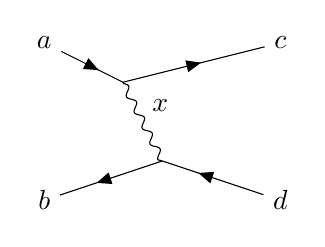
\begin{tikzpicture}[baseline=(current bounding box)]
            \begin{feynman}
                \vertex (i1) at (0, 1) {\(a\)};
                \vertex (i2) at (0, -1) {\(b\)};
                \vertex (v1) at (1, 0.5);
                \vertex (v2) at (1.5, -0.5);
                \vertex (o1) at (3, 1) {\(c\)};
                \vertex (o2) at (3, -1) {\(d\)};
                \diagram* [small] {
                    (i1) -- [fermion] (v1) -- [fermion] (o1),
                    (i2) -- [anti fermion] (v2) -- [anti fermion] (o2),
                    (v1) -- [photon, edge label=\(x\)] (v2)
                };
            \end{feynman}
        \end{tikzpicture}
    \end{equation}
    
    We then have three states, the initial state, \(\ket{a, b}\), the intermediate state, \(\ket{c, x, b}\), and the final state \(\ket{c, d}\).
    The energy of the initial state is \(E_a + E_b\), and the energy of the intermediate state is \(E_c + E_x + E_b\).
    Putting this together we get the contribution to the second term from this time ordering:
    \begin{equation}
        T_{fi}^{ab} = \frac{\bra{c, d} V \ket{c, x, b} \bra{c, x, b} V \ket{a, b}}{(E_a + E_b) - (E_c + E_x + E_b)} = \frac{\bra{c, d} V \ket{c, x, b} \bra{c, x, b} V \ket{a, b}}{E_a - E_c - E_x}.
    \end{equation}
    Here we write \(T_{fi}^{ab}\) for the process \(a + b \to c + d\) specifically time ordered so that \(a\) emits a particle which is then absorbed by \(x\).
    
    Recall that \(T_{fi}\) is given by the amplitude, \(\amplitude_{fi}\), divided by the square root of the product of twice the energies of all particles in the initial and final state.
    We can use this to work out the amplitudes \(\bra{c, d} V \ket{c, x, b}\) and \(\bra{c, x, b} V \ket{a, b}\), which are just transition matrix elements for the processes \(x + b \to d\) and \(a \to c + x\) respectively.
    We then have
    \begin{equation}
        \bra{c, d} V \ket{c, x, b} = \frac{\amplitude_{fi}^{a \to c + x}}{\sqrt{2E_a2E_c2E_x}} = \frac{g_a}{\sqrt{2E_a2E_c2E_x}},
    \end{equation}
    where \(g_a\) measures the strength of the interaction \(a \to c + x\).
    Similarly,
    \begin{equation}
        \bra{c, x, b} V \ket{a, b} = \frac{\amplitude_{fi}^{x + b \to d}}{\sqrt{2E_d2E_x2E_b}} = \frac{g_b}{\sqrt{2E_d2E_x2E_b}},
    \end{equation}
    where \(g_b\) measures the strength of the interaction \(x + b \to d\).
    
    We can then compute the total amplitude for this particular time ordering of this process.
    First we compute the total transition matrix element:
    \begin{equation}
        T_{fi}^{ab} = \frac{g_ag_b}{2E_x\sqrt{2E_a2E_b2E_c2E_d}} \frac{1}{\sqrt{E_a - E_x - E_c}},
    \end{equation}
    and then the amplitude is
    \begin{equation}
        \amplitude_{fi}^{ab} = g_ag_b \sqrt{2E_a2E_b2E_c2E_d} T_{fi}^{ab} = \frac{g_ag_b}{2E_x(E_a - E_c - E_x)}.
    \end{equation}
    Note that \(\amplitude_{fi}^{ab}\) is \emph{not} Lorentz invariant, since we are explicitly defining a time ordering for the processes occurring, which a Lorentz transformation may change.
    
    We can similarly consider the process where \(b\) emits the antiparticle \(\overbar{x}\), which is then absorbed by \(a\):
    \begin{equation}
        \tikzsetnextfilename{fd-electron-positron-scattering-alternate-order}
        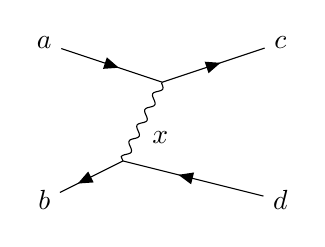
\begin{tikzpicture}[baseline=(current bounding box)]
            \begin{feynman}
                \vertex (i1) at (0, 1) {\(a\)};
                \vertex (i2) at (0, -1) {\(b\)};
                \vertex (v1) at (1.5, 0.5);
                \vertex (v2) at (1, -0.5);
                \vertex (o1) at (3, 1) {\(c\)};
                \vertex (o2) at (3, -1) {\(d\)};
                \diagram* [small] {
                    (i1) -- [fermion] (v1) -- [fermion] (o1),
                    (i2) -- [anti fermion] (v2) -- [anti fermion] (o2),
                    (v1) -- [photon, edge label=\(\overbar{x}\)] (v2)
                };
            \end{feynman}
        \end{tikzpicture}
    \end{equation}
    An identical calculation gives
    \begin{equation}
        \amplitude_{fi}^{ba} = \frac{g_ag_b}{2E_x(E_b - E_d - E_x)}.
    \end{equation}
    
    The total amplitude for this \(t\)-channel process is
    \begin{align}
        \amplitude_{fi}^t &= \amplitude_{fi}^{ab} + \amplitude_{fi}^{ba}\\
        &= \frac{g_ag_b}{2E_x}\left( \frac{1}{E_a - E_c - E_x} + \frac{1}{E_b - E_d - E_x} \right).
    \end{align}
    Conservation of energy tells us that \(E_a + E_b = E_c + E_d\), and so we can write this as
    \begin{align}
        \amplitude_{fi}^t &= \frac{g_ag_b}{2E_x}\left( \frac{1}{E_a - E_c - E_x} - \frac{1}{E_a - E_c + E_x} \right)\\
        &= \frac{g_ag_b}{2E_x} \frac{2E_x}{(E_a - E_c)^2 - E_x^2}\\
        &= \frac{g_ag_b}{(E_a - E_c)^2 - E_x^2}.
    \end{align}
    The relativistic energy-momentum relation tells us that \(E_x^2 = \vv{p_x}^2 + m_x^2\) and if we consider the first time ordering then we have \(\vv{p_x} = \vv{p_a} - \vv{p_c}\), so
    \begin{align}
        \amplitude_{fi}^t &= \frac{g_ag_b}{(E_a - E_c)^2 - (\vv{p_a} - \vv{p_c})^2 - m_x^2}\\
        &= \frac{g_ag_b}{(p_a - p_b)^2 - m_x}\\
        &= \frac{g_ag_b}{q^2 - m_x^2}\\
        &= \frac{g_ag_b}{t - m_x^2}.
    \end{align}
    Here \(q = p_a - p_c\) is the four-momentum of the exchange particle and \(t\) is the Mandelstam invariant.
    This is a fairly common form for the amplitude to take.
    
    Notice that we do \emph{not} require \(q^2 = m_x^2\), in fact, if this were the case then the amplitude would be singular.
    Suppose we have elastic scattering, then \(p_a = (E, \vv{p_a})\) and \(p_c = (E, \vv{p_c})\), and so we have
    \begin{equation}
        q^2 = (p_a - p_c)^2 = (E - E)^2 - (\vv{p_a} - \vv{p_c})^2 = -(\vv{p_a} - \vv{p_c})^2 \le 0.
    \end{equation}
    So we don't even need to have \(q^2\) be positive.
    This is all because \(x\) is a \defineindex{virtual particle}, which is a particle which is \defineindex{off-shell}, meaning \(q^2 \ne m_x^2\).
    If \(q^2 = m_x^2\) then we say that the particle is \defineindex{on-shell}.
    We cannot have virtual particles in the initial and final states, but there perfectly valid intermediate states.
    This is mostly just an artefact of us reading too literally into what's happening in a process defined by a Feynman diagram.
    
    \part{QED}    
    \chapter{Quantum Electrodynamics}
    \section{Modifying the Dirac Equation}
    We can modify the Dirac equation to allow for electromagnetic interactions by the \defineindex{minimal coupling prescription}\footnote{See \course{Quantum Theory}}, where we modify the momentum and energy according to
    \begin{equation}
        \vv{p} \mapsto \vv{p} - q\vv{A}, \qqand E \mapsto E - q\varphi
    \end{equation}
    where \(q\) is the charge of the particle, \(\vv{A}\) is the vector potential and \(\varphi\) the electrostatic potential.
    We can write this modification as
    \begin{equation}
        p^\mu \mapsto p^\mu - qA^\mu
    \end{equation}
    where \(A^\mu = (\varphi, \vv{A})\) is the four-potential\footnote{See \course{Classical Electrodynamics}}.
    We then make the corresponding modification to the quantum mechanical operators, \(\vv{p} = -i\grad\) and \(E = i\partial_t\), or \(p^\mu = i\partial^\mu\) to get
    \begin{equation}
        p^\mu = i\partial^\mu \mapsto p^\mu - qA^\mu = i\partial^\mu - qA^\mu.
    \end{equation}
    Hence, the Dirac equation in the presence of an electric field is modified according to
    \begin{equation}
        (i\slashed{\partial} - m)\psi = 0 \mapsto (i\slashed{\partial} - q\slashed{A} - m)\psi = 0.
    \end{equation}
    
    As motivation consider what we get if we rearrange this slightly.
    First multiply through by \(\gamma^0\) to get
    \begin{equation}
        i\gamma^0 \slashed{\partial}\psi - q\gamma^0\slashed{A}\psi - m\gamma^0\psi = 0.
    \end{equation}
    Then using \((\gamma^0)^2 = 1\) we have
    \begin{align}
        0 &= i\gamma^0\slashed{\partial}\psi - q\gamma^0\slashed{A}\psi - m\gamma^0\psi\\
        &= i\gamma^0\gamma^\mu\partial_\mu\psi - q\gamma^0\slashed{A}\psi - m\gamma^0\psi\\
        &= i(\gamma^0)^2\partial_t\psi - i\gamma^0\gamma^i\partial_i\psi - q\gamma^0\slashed{A} - m\gamma^0\psi\\
        &= i\diffp{\psi}{t} - i\gamma^0\vv{\gamma} \cdot \grad\psi - q\gamma^0 \slashed{A} - m\gamma^0\psi.
    \end{align}
    Moving the first term to the other side we have
    \begin{equation}
        i\diffp{\psi}{t} = i\gamma^0\vv{\gamma} \cdot \grad \psi + m\gamma^0\psi + q\gamma^0\slashed{A}.
    \end{equation}
    We then interpret the left hand side, \(i\partial_t \psi\), as the Hamiltonian acting on the spinor, \(\operator{H}\psi\).
    The terms on the right then correspond to the kinetic energy, mass-energy, and potential energy respectively.
    
    We can then write the potential energy operator for a spinor satisfying the Dirac equation in an electromagnetic field as
    \begin{equation}
        V_{\dirac} = q \gamma^0\slashed{A}.
    \end{equation}
    Note that the time-like contribution, \(\mu = 0\), to \(q\gamma^0\gamma^\mu A_\mu\) is \(q(\gamma^0)^2A_0 = q\varphi\), which is just the usual electrostatic potential.
    
    \section{Photons}
    Before we get to the calculation we should consider what's happening in the interaction.
    We start with two fermions, these are described by the Dirac equation.
    We end with two fermions, also described by the Dirac equation.
    In between we'll have a photon, which is a spin 1 boson.
    Noninteracting photons are described by Maxwell's equation\footnote{for relativistic use of Maxwell's equations see \course{Classical Electrodynamics}, for use in relativistic quantum theory see \course{Quantum Field Theory}}, \(\dalembertian A^\nu - \partial^\nu\partial_\mu A^\mu = 0\).
    This has plane wave solutions,
    \begin{equation}
        A_\mu = \varepsilon_\mu^{(\lambda)} \e^{-ip\cdot x}.
    \end{equation}
    Here \(\varepsilon_\mu^{(\lambda)}\) is the polarisation vector, with \(\lambda\) labelling the polarisation state.
    This is just a normal four vector, since \(A_\mu\) is just a four-vector.
    Since polarisation is a purely spatial phenomenon the time component of \(\varepsilon^{(\lambda)}\) is zero (at least we can always choose for it to be such).
    For massless particles, like the photon, it's not possible for them to be polarised in the direction of travel, since this would, intuitively, require the field to oscillate in the direction of travel, so when oscillating forward it would propagate a signal faster than the speed of light.
    There are therefore two polarisation states,
    \begin{equation}
        \varepsilon^{(1)} = 
        \begin{pmatrix}
            0\\ 1\\ 0\\ 0
        \end{pmatrix}
        , \qqand \varepsilon^{(2)} = 
        \begin{pmatrix}
            0\\ 0\\ 1\\ 0
        \end{pmatrix}
        .
    \end{equation}
    A virtual photon has two more polarisation states, it can be polarised in the time direction or in the direction of travel, corresponding to the states
    \begin{equation}
        \varepsilon^{(0)} = 
        \begin{pmatrix}
            1\\ 0\\ 0\\ 0
        \end{pmatrix}
        , \qqand \varepsilon^{(3)} = 
        \begin{pmatrix}
            0\\ 0\\ 0\\ 1
        \end{pmatrix}
    \end{equation}
    respectively.
    A general photon state will be a superposition of polarisations, meaning the solution will be of the form
    \begin{equation}
        A^\mu = \sum_\lambda \varepsilon_\mu^{(\lambda)} \e^{-ip\cdot x}.
    \end{equation}
    
    \section{Calculating the Amplitude}
    Recall that the amplitude for \(t\)-channel scattering \(a + b \to c + d\) is
    \begin{equation}
        \amplitude_{fi}^t = \frac{g_ag_b}{q^2 - m_x^2}.
    \end{equation}
    The values \(g_a\) and \(g_b\) are supposed to stand for the strength of the interactions \(a \to x + c\) and \(x + b \to d\) respectively.
    They are simply the matrix elements for these processes:
    \begin{equation}
        g_a = \bra{\psi_c} V \ket{\psi_a}, \qqand g_b = \bra{\psi_d} V \ket{\psi_b}.
    \end{equation}
    Here \(\ket{\psi}\) is the spinor state corresponding to the relevant particles.
    
    We now consider the process \(\Pe\Ptau \to \Pe\Ptau\) via a single photon as an intermediate state in a \(t\)-channel diagram.
    Since the exchange particle is a photon it is massless, and so we can replace the \(1/(q^2 - m_x^2)\) term with \(1/q^2\).
    The potential is replaced with the potential \(V_{\dirac} = q\gamma^0\slashed{A}\).
    The initial state corresponds to an electron and a tau particle, and so does the final state, although the momenta may have changed (although the total momentum is of course conserved).
    Hence,
    \begin{equation}
        g_{\Pe} = \bra{\psi_{\Pe,c}} V \ket{\psi_{\Pe,a}}.
    \end{equation}
    The state for the electron before and after then interaction is
    \begin{equation}
        \ket{\psi_{\Pe,a}} = u(p_a), \qqand \ket{\psi_{\Pe,c}} = u(p_c).
    \end{equation}
    Hence, we have
    \begin{equation}\label{eqn:electron-photon interaction strength}
        g_{\Pe} = u^\hermit(p_c) e\gamma^0\slashed{A} u(p_a) = e\diracadjoint{u}(p_c) \slashed{A} u(p_a).
    \end{equation}
    Similarly for the tau particle we have
    \begin{equation}
        g_{\Ptau} = e\diracadjoint{u}(p_d) \slashed{A}^* u(p_b).
    \end{equation}
    The only difference is the complex conjugate here.
    This arises because one particle emits the photon and the other absorbs it, however these processes are related by time reversal, and when we reverse time phase factors change as
    \begin{equation}
        \e^{-iEt} \mapsto \e^{-iE(-t)} = \e^{iEt} = (\e^{-iEt})^*,
    \end{equation}
    so we have to take complex conjugates\footnote{See \course{Quantum Field Theory} for details}.
    We don't know which of the particles absorbs the photon and which emits it, but it doesn't matter, the important thing is the relative complex conjugate.
    Putting this together we have
    \begin{equation}
        \amplitude_{fi}^{t} = e^2\diracadjoint{u}(p_c) \gamma^0\slashed{A} u(p_b) \frac{1}{q^2} \diracadjoint{u}(p_d) \gamma^0\slashed{A}^* u(p_d).
    \end{equation}
    Now we can deal with the \(\slashed{A}\) terms.
    First notice that \(A_\mu\) is just a number, its the component of some four-vector, and so commutes with everything.
    Since it is the same photon that leaves one particle and is absorbed by the other, with no other interactions, its polarisation cannot change.
    This means that our sum over polarisations should be just a single sum, rather than summing each factor of \(A_\mu\) over polarisations, so we have
    \begin{equation}
        A_\mu A_\nu^* = \sum_{\lambda} \varepsilon_\mu^{(\lambda)}\e^{-ip\cdot x}(\varepsilon_\nu^{(\lambda)} \e^{-ip\cdot x})^* = \sum_{\lambda} \varepsilon_\mu^{(\lambda)} (\varepsilon_\nu^{(\lambda)})^*.
    \end{equation}
    We then have
    \begin{align}
        \amplitude_{fi}^t &= e^2 \diracadjoint{u}(p_c) \gamma^0\gamma^\mu A_\mu u(p_b) \frac{1}{q^2} \diracadjoint{u}(p_d) \gamma^0\gamma^\nu A_\nu^* u(p_d)\\
        &= \sum_\lambda e^2 \diracadjoint{u}(p_c) \gamma^0 \gamma^\mu u(p_b) \frac{\varepsilon_\mu^{(\lambda)} \varepsilon_\nu^{(\lambda)}}{q^2} \diracadjoint{u}(p_d) \gamma^0\gamma^\nu u(p_d)\\
        &= -e^2 \diracadjoint{u}(p_c) \gamma^0 \gamma^\mu u(p_b) \frac{\minkowskiMetric_{\mu\nu}}{q^2} \diracadjoint{u}(p_d) \gamma^0\gamma^\nu u(p_d).\label{eqn:electron tau scattering amplitude}
    \end{align}
    In the last step we used the result
    \begin{equation}
        \sum_\lambda \varepsilon_\mu^{(\lambda)}(\varepsilon_\nu)^{(\lambda)} = -g_{\mu\nu}
    \end{equation}
    derived in \cref{eqn:spin sum}.
    
    \section{Feynman Rules}\label{sec:feynman rules QED}
    Good news!
    We don't have to do this calculation every time.
    Instead, since the process is relatively formulaic, we can use \defineindex{Feynman rules} which allow us to look at a Feynman diagram and convert it into the matrix element.
    The exact Feynman rules depend on what theory we're considering, so here we'll do the Feynman rules for QED.
    
    There are three parts to the Feynman rules\footnote{We do not concern ourselves with symmetry factors here, which form a fourth part to the Feynman rules, see \course{Quantum Field Theory} for details.}.
    We have a rule for each external line, that is a line representing a real particle, a rule for each internal particle, that is a virtual particle, and a rule for each vertex.
    The rules for the lines depend on the momentum of the particle, and the type of particle.
    We also give each vertex a Lorentz index, and the rules may depend on the indices at either end of the line, and the vertex term will also typically depend on the index of the vertex.
    
    So, without further ado here are the Feynman rules for QED.
    First, we have the rules for spin \(1/2\) external (anti)particles with momentum \(p\), note that \tikzsetnextfilename{fd-dot-vertex-1}\feynmandiagram{a [dot]}; corresponds to a vertex, whereas a lack of a \tikzsetnextfilename{fd-dot-vertex-2}\feynmandiagram{a [dot]}; corresponds to an external particle:
    \begin{equation}
        \begin{array}{rrr}
            \text{Incoming particle} & u(p) & \tikzsetnextfilename{fd-incoming-fermion}\feynmandiagram[horizontal=a to b]{a -- [fermion] b [dot]}; \\
            \text{Outgoing particle} & \diracadjoint{u}(p) & \tikzsetnextfilename{fd-outgoing-fermion}\feynmandiagram[horizontal=a to b]{a [dot] -- [fermion] b}; \\
            \text{Incoming antiparticle} & \diracadjoint{v}(p) & \tikzsetnextfilename{fd-incoming-antifermion}\feynmandiagram[horizontal=a to b]{a -- [anti fermion] b [dot]}; \\
            \text{Outgoing antiparticle} & v(p) & \tikzsetnextfilename{fd-outgoing-antifermion}\feynmandiagram[horizontal=a to b]{a [dot] -- [anti fermion] b};
        \end{array}
    \end{equation}

    Next, we have the rules for spin 1 external particles, which in QED is just photons.
    For a photon with momentum \(p\) the rules are as follows:
    \begin{equation}
        \begin{array}{rrr}
            \text{Incoming photon} & \varepsilon^\mu(p) & \tikzsetnextfilename{fd-incoming-photon}\feynmandiagram[horizontal=a to b]{a -- [photon] b [dot]}; \, \mu \\
            \text{Outgoing photon} & \varepsilon^\mu(p)^* & \mu \, \tikzsetnextfilename{fd-outgoing-photon}\feynmandiagram[horizontal=a to b]{a [dot] -- [photon] b};
        \end{array}
    \end{equation}
    Then there are internal lines, we've already seen the photon propagator, for an internal photon of momentum \(q\):
    \begin{equation}
        \begin{array}{rrr}
            \text{Photon propagator} & \displaystyle-\frac{i\minkowskiMetric_{\mu\nu}}{q^2} & \mu \, \tikzsetnextfilename{fd-internal-photon}\feynmandiagram[horizontal=a to b]{a [dot] -- [photon] b [dot]}; \, \nu
        \end{array}
    \end{equation}
    For a spin \(1/2\) fermion propagator of mass \(m\) and momentum \(q\) we have
    \begin{equation}
        \begin{array}{rrr}
            \text{Photon propagator} & \displaystyle-\frac{i(\slashed{q} + m)}{q^2 - m^2} & \tikzsetnextfilename{fd-internal-fermion}\feynmandiagram[horizontal=a to b]{a [dot] -- b [dot]};
        \end{array}
    \end{equation}
    Finally we have a vertex factor.
    We've only considered vertices with two fermions and a photon so far, so for a fermion of charge \(-e\), where \(e\) is the magnitude of the charge of the electron, we have the following rule:
    \begin{equation}
        \begin{array}{rrr}
            \text{Vertex} & ie\gamma^\mu & 
            \tikzsetnextfilename{fd-vertex-factor}
            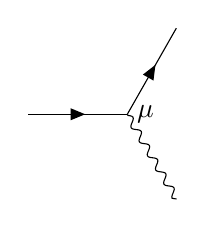
\begin{tikzpicture}[baseline=(mu.base)]
                \begin{feynman}
                    \diagram[horizontal=a to v, small]{
                        a -- [fermion] v -- [fermion] b,
                        v -- [photon] c
                    };
                    \node[right] (mu) at (v) {\(\mu\)};
                \end{feynman}
            \end{tikzpicture}
        \end{array}
    \end{equation}
    
    We find the amplitude from the Feynman rules by multiplying together all of the terms appearing in the diagram, which gives \(-i\amplitude\).
    
    \subsection{Using the Feynman Rules}
    We can consider the following diagram again:
    \begin{equation}
        \vcenter{\hbox{\includegraphics{tikz-external/fd-electron-tau-scattering}}}
    \end{equation}
    Call the top vertex \(\mu\) and the bottom one \(\nu\).
    At the top vertex we have an incoming electron, corresponding to a factor of \(u(p_a)\), a vertex factor, \(ie\gamma^\mu\), and an outgoing electron, corresponding to a factor of \(\diracadjoint{u}(p_c)\).
    Similarly at the bottom vertex we get \(\diracadjoint{u}(p_d) ie\gamma^\nu u(p_b)\).
    We also have a photon propagator giving a factor of \(-i\minkowskiMetric/q^2\).
    So we recover the result
    \begin{equation}
        -i\amplitude = ie^2\diracadjoint{u}(p_c) \gamma^\nu u(p_a) \frac{\minkowskiMetric_{\mu\nu}}{q^2} \diracadjoint{u}(p_d) \gamma^\nu u(p_b).
    \end{equation}
    
    \chapter{\texorpdfstring{\(\APe\Pe \to \APmu\Pmu\)}{Electron Positron to Muon Antimuon}}
    \label{chap:electron-positron to muon-antimuon}
    \section{Setup}
    In this chapter we'll calculate the cross section for the interaction
    \begin{equation}
        \APe\Pe \to \APmu \Pmu
    \end{equation}
    to lowest order in QED.
    Since the particles change the lowest order process has a single internal particle, and since this is QED it will be a photon.
    Note that this calculation is repeated in \cref{sec:electron-positron to muon-antimuon with feyncalc} using the \textit{Mathematica} packages \textit{FeynCalc} and \textit{FeynArt} to do most of the work.
    
    In the lab this process may look like
    \begin{equation}
        \tikzsetnextfilename{lab-view-of-ee-mumu}
        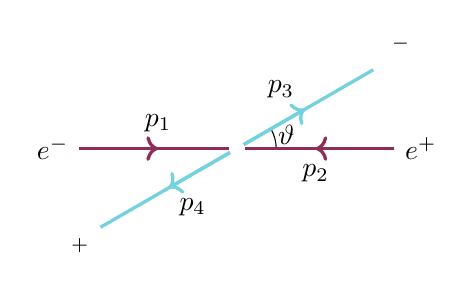
\begin{tikzpicture}[baseline=-0.1]
            \path (2, 0) coordinate (A) -- (0, 0) coordinate (B) -- (30:2) coordinate (C) pic [draw, "\(\vartheta\)", angle eccentricity=1.3] {angle};
            \draw[Burgandy, very thick] (-2, 0) node [left, text=black] {\Pe} -- (-0.1, 0);
            \draw[Burgandy, very thick, ->] (-2, 0) -- (-1, 0) node [above, text=black, yshift=2pt] {\(p_1\)};
            \draw[Burgandy, very thick] (2, 0) node [right, text=black] {\APe} -- (0.1, 0);
            \draw[Burgandy, very thick, ->] (2, 0) -- (1, 0) node [below, text=black, yshift=-2pt] {\(p_2\)};
            \draw[Blue, very thick] (30:0.1) -- (30:2) node [above right, text=black] {\Pmu};
            \draw[Blue, very thick, ->] (30:0.1) -- (30:1) node [above left, text=black] {\(p_3\)};
            \draw[Blue, very thick] (210:0.1) -- (210:2) node [below left, text=black] {\APmu};
            \draw[Blue, very thick, ->] (210:0.1) -- (210:1) node [below right, text=black] {\(p_4\)};
        \end{tikzpicture}
    \end{equation}
    We assume that the electron and positron beams have the same energy, \(E\), and then the muon and antimuon must also have energy \(E\) as total energy must be conserved and symmetries demands that the energy is shared evenly between the two particles.
    In the centre of mass frame the momenta of the particles are
    \begin{equation*}
        p_1 = (E, 0, 0, p), \quad p_2 = (E, 0, 0, -p), \quad p_3 = (E, \vv{p_f}), \qand p_4 = (E, -\vv{p_f})
    \end{equation*}
    where \(\vv{p_f}\) has magnitude \(p\) and is at an angle \(\vartheta\) to the \(z\)-axis, which we take to be the axis along which the beams travel.
    We'll assume that the interaction occurs at high energies, so \(m \ll E\) and \(\abs{\vv{p}} \approx E\) so we can neglect the masses in most equations.
    
    
    \section{Feynman Diagram and Amplitude}
    We consider only the lowest order diagram for this process.
    We also restrict ourselves to QED, if this wasn't the case then the internal propagator could also be a \PZ{} boson, or a Higgs boson.
    Since the particles change this is necessarily a second order process.
    There are two second order diagrams, \(s\), \(t\), and \(u\)-channel.
    Since this is an annihilation interaction producing different products to the incoming particles it can only proceed via an \(s\)-channel process.
    So we consider the diagram
    \begin{equation}
        \tikzsetnextfilename{fd-elecron-positron-to-muon-antimuon}
        \feynmandiagram[horizontal=v1 to v2, inline=(v1)]{
            i1 [particle=\Pe] -- [fermion] v1,
            i2 [particle=\APe] -- [anti fermion] v1,
            v1 -- [photon] v2,
            v2 -- [fermion] o1 [particle=\Pmu],
            v2 -- [anti fermion] o2 [particle=\APmu]
        };
    \end{equation}
    
    We can convert this into an amplitude using the Feynman rules for QED.
    First focus on the incoming particles, we have an electron, giving a factor of \(u(p_1)\), then a vertex giving a factor of \(ie\gamma^\mu\), and then an antielectron, giving a factor of \(\diracadjoint{v}(p_2)\).
    The photon propagator gives a factor of \(-i\minkowskiMetric_{\mu\nu}/q^2\).
    The outgoing muon gives a factor of \(\diracadjoint{u}(p_3)\), the vertex gives a factor of \(ie\gamma^\nu\) and the outgoing antimuon gives a factor of \(v(p_4)\).
    
    Combining this we have the amplitude
    \begin{align}
        -i\amplitude &= [\diracadjoint{v}(p_2) i\varepsilon \gamma^\mu u(p_1)] \left( -\frac{i\minkowskiMetric_{\mu\nu}}{q^2} \right) [\diracadjoint{u}(p_3) ie\gamma^\nu v(p_4)]\\
        \amplitude &= -\frac{e^2}{q^2} \minkowskiMetric_{\mu\nu} \diracadjoint{v}(p_2) \gamma^\mu u(p_1) \diracadjoint{u}(p_3) \gamma^\nu v(p_4)\\
        &= -\frac{e^2}{q^2} j_{\symrm{e}} \cdot j_{\text{μ}}\\
        &= -\frac{e^2}{s} j_{\symrm{e}} \cdot j_{\text{μ}}
    \end{align}
    where
    \begin{equation}
        j_{\symrm{e}} = \diracadjoint{v}(p_2) \gamma^\mu u(p_1), \qqand j_{\text{μ}} = \diracadjoint{u}(p_3) \gamma^\nu v(p_4).
    \end{equation}
    
    \section{Spin}
    In general the electrons and positrons won't be polarised, instead we expect an even mix of left and right helicity states.
    This means that there are four options for the incoming helicity, \(RL\), \(RR\), \(LL\), and \(LR\), where the first letter is the helicity of the electron and the second the helicity of the positron.
    There are then 16 possible helicity combinations, since the helicity of the muon and antimuon can also take these four values.
    
    The helicity of the final particles is something to measure.
    The helicity of the initial states must be averaged over, so we have
    \begin{align}
        \expected{\abs{\amplitude}^2} &= \frac{1}{4} \sum_{\text{helicities}} \abs{M_i}^2\\
        &= (\abs{\amplitude_{LL \to LL}}^2 + \abs{\amplitude_{LL \to LR}}^2 + \abs{\amplitude_{LL \to RL}}^2 + \abs{\amplitude_{LL \to RR}}^2\\
        &\qquad + \abs{\amplitude_{LR \to LL}}^2 + \abs{\amplitude_{LR \to LR}} + \dotsb).
    \end{align}
    
    Now consider the helicity spinors
    \begin{alignat}{2}
        u_{\uparrow} &= \sqrt{E}
        \begin{pmatrix}
            c\\ s\e^{i\varphi}\\ c\\ s\e^{i\varphi}
        \end{pmatrix}
        , \qquad & u_{\downarrow} &= \sqrt{E}
        \begin{pmatrix}
            -s\\ \e^{i\varphi}\\ s\\ -c\e^{i\varphi}
        \end{pmatrix}
        ,\\
        v_{\uparrow} &= \sqrt{E}
        \begin{pmatrix}
            s\\ -c\e^{i\varphi}\\ -s\\ c\e^{i\varphi}
        \end{pmatrix}
        ,\qquad & v_{\downarrow} &= \sqrt{E}
        \begin{pmatrix}
            c\\ s\e^{i\varphi}\\ c\\ s\e^{i\varphi}
        \end{pmatrix}
    \end{alignat}
    where \(c = \cos(\Theta/2)\) and \(s = \sin(\Theta/2)\), where \(\Theta\) is the polar angle defining the direction of momentum, and we've assumed \(E \gg m\).
    
    We choose to define our coordinates so that the electron moves along the \(z\)-axis, then the polar angle for the electron is \(0\), the polar angle for the positron is \(\pi\), the polar angle for the muon is \(\vartheta\), and the polar angle for the antimuon is \(\pi - \vartheta\).
    The particles move in a plane, which we may as well take to be the \((x,y)\)-plane, so that \(\varphi = 0, \pi\), depending on the direction.
    
    The initial electron can be in either a left or right-handed helicity state and with \(\Theta = 0\) and \(\varphi = 0\) this gives the two possible states
    \begin{equation}
        u_{\uparrow}(p_1) = \sqrt{E}
        \begin{pmatrix}
            1\\ 0\\ 1\\ 0
        \end{pmatrix}
        , \qqor u_{\downarrow}(p_1) = \sqrt{E}
        \begin{pmatrix}
            0\\ 1\\ 0\\ -1
        \end{pmatrix}
        .
    \end{equation}
    Similarly the positron can be left or right-handed, and with \(\Theta = \pi\) and \(\varphi = 0\) this gives
    \begin{equation}
        v_{\uparrow}(p_2) = \sqrt{E}
        \begin{pmatrix}
            1\\ 0\\ -1\\ 0
        \end{pmatrix}
        , \qqor v_{\downarrow}(p_2) = \sqrt{E}
        \begin{pmatrix}
            0\\ 1\\ 0\\ 1
        \end{pmatrix}
        .
    \end{equation}
    The muon has polar angle \(\Theta = \vartheta\) and \(\varphi = 0\) giving possible states
    \begin{equation}
        u_{\uparrow}(p_3) = \sqrt{E}
        \begin{pmatrix}
            c\\ s\\ c\\ s
        \end{pmatrix}
        , \qqor u_{\downarrow}(p_3) = \sqrt{E}
        \begin{pmatrix}
            -s\\ c\\ s\\ -c
        \end{pmatrix}
        ,
    \end{equation}
    where \(c = \cos(\vartheta/2)\) and \(s = \sin(\vartheta/2)\).
    Finally, for the antimuon we have \(\Theta = \pi - \vartheta\) and \(\varphi = \pi\), and we can use the identities \(\sin([\pi - \vartheta]/2) = \cos(\vartheta/2)\) and \(\cos([\pi - \vartheta]/2) = \sin(\vartheta/2)\).
    Hence, the possible states of the antimuon are
    \begin{equation}
        v_{\uparrow}(p_4) = \sqrt{E}
        \begin{pmatrix}
            c\\ s\\ -c\\ -s
        \end{pmatrix}
        , \qqor v_{\downarrow}(p_4) = \sqrt{E}
        \begin{pmatrix}
            -s\\ c\\ s\\ -c
        \end{pmatrix}
        .
    \end{equation}
    
    \section{Muon Current}
    We want to evaluate the muon current,
    \begin{equation}
        (j_{\text{μ}})^\nu = \diracadjoint{u}(p_3)\gamma^\nu v(p_4),
    \end{equation}
    for each helicity combination.
    To start with we need a few identities.
    For arbitrary four-component spinors, \(\Psi\) and \(\Phi\), in the Dirac representation we have
    \begin{align}
        \diracadjoint{\Psi} \gamma^0 \Phi &= \Psi^\hermit \gamma^0 \gamma^0 \Phi = \Psi_1^* \Phi_1 + \Psi_2^*\Phi_2 + \Psi_3^*\Phi_3 + \Psi_4^*\Phi_4,\\
        \diracadjoint{\Psi} \gamma^1 \Phi &= \Psi^\hermit \gamma^0 \gamma^1 \Phi = \Psi_1^* \Phi_4 + \Psi_2^*\Phi_3 + \Psi_3^*\Phi_2 + \Psi_4^*\Phi_1,\\
        \diracadjoint{\Psi} \gamma^2 \Phi &= \Psi^\hermit \gamma^0 \gamma^2 \Phi = -i(\Psi_1^* \Phi_4 - \Psi_2^*\Phi_3 + \Psi_3^*\Phi_2 - \Psi_4^*\Phi_1,\\
        \diracadjoint{\Psi} \gamma^4 \Phi &= \Psi^\hermit \gamma^0 \gamma^4 \Phi = \Psi_1^* \Phi_3 - \Psi_2^*\Phi_4 + \Psi_3^*\Phi_1 - \Psi_4^*\Phi_2.\\
    \end{align}
    These follow by writing
    \begin{equation}
        \Psi^\hermit = 
        \begin{pmatrix}
            \Psi_1^* & \Psi_2^* & \Psi_3^* & \Psi_4^*
        \end{pmatrix}
        , \qqand 
        \Phi = 
        \begin{pmatrix}
            \Phi_1\\ \Phi_2\\ \Phi_3\\ \Phi_4
        \end{pmatrix}
        ,
    \end{equation}
    and then computing the matrix products.
    
    Consider the case where the muon is right-handed and the antimuon is left-handed.
    Then we have \(\Psi = u_{\uparrow}\) and \(\Phi = v_{\downarrow}\) giving
    \begin{align}
        \diracadjoint{u}_{\uparrow} \gamma^0 \diracadjoint{v}_{\downarrow} &= E(cs - sc + cs - sc) = 0,\\
        \diracadjoint{u}_{\uparrow} \gamma^1 \diracadjoint{v}_{\downarrow} &= E(-c^2 + s^2 - c^2 + s^2) = 2E(s^2 - c^2) = -2E\cos\vartheta,\\
        \diracadjoint{u}_{\uparrow} \gamma^2 \diracadjoint{v}_{\downarrow} &= -iE(-c^2 - s^2 - c^2 - s^2) = 2iE,\\
        \diracadjoint{u}_{\uparrow} \gamma^3 \diracadjoint{v}_{\downarrow} &= E(cs + sc + cs + sc) = 4Ecs = 2E\sin\vartheta.
    \end{align}
    The four-vector current for the \(RL\) helicity combination is
    \begin{equation}
        \diracadjoint{u}_{\uparrow} \gamma^\nu \diracadjoint{v}_{\downarrow} = 2E(0, -\cos\vartheta, i, \sin\vartheta).
    \end{equation}
    
    Doing the same with the other helicity combinations we get the results
    \begin{align}
        RL: \qquad &\diracadjoint{u}_{\uparrow}(p_3) \gamma^\nu \diracadjoint{v}_{\downarrow}(p_4) = 2E(0, -\cos\vartheta, i, \sin\vartheta),\\
        RR: \qquad &\diracadjoint{u}_{\uparrow}(p_3) \gamma^\nu \diracadjoint{v}_{\uparrow}(p_4) = (0, 0, 0, 0),\\
        LL: \qquad &\diracadjoint{u}_{\downarrow}(p_3) \gamma^\nu \diracadjoint{v}_{\uparrow}(p_4) = (0, 0, 0, 0),\\
        LR: \qquad &\diracadjoint{u}_{\downarrow}(p_3) \gamma^\nu \diracadjoint{v}_{\downarrow}(p_4) = 2E(0, -\cos\vartheta, -i, \sin\vartheta).
    \end{align}
    We see that, in the limit where \(E \gg m\), only two helicity states are nonzero.
    
    \section{Electron Current}
    The electron current can be computed using the muon current by noticing that
    \begin{align}
        [\diracadjoint{u}(p_3)\gamma^\nu v(p_4)]^\hermit &= [u^\hermit(p_3)\gamma^0\gamma^\nu v(p_4)]^\hermit\\
        &= v^\hermit(p_4) (\gamma^\nu)^\hermit (\gamma^0)^\hermit u(p_3)\\
        &= v^\hermit(p_4) (\gamma^\nu)^\hermit \gamma^0 u(p_3)\\
        &= v^\hermit(p_4) \gamma^0 \gamma^\nu u(p_3)\\
        &= \diracadjoint{v}(p_4) \gamma^0 \gamma^\nu u(p_3).
    \end{align}
    This follows since \((\gamma^0)^\hermit = \gamma^0\), and \(\gamma^0\gamma^\mu\gamma^0 = (\gamma^\mu)^\hermit\), which can be written as \((\gamma^\mu)^\hermit\gamma^0 = \gamma^0\gamma^\mu\) using \((\gamma^0)^2 = 1\).
    
    This means that if we take the complex conjugate of the muon current we get the same form as the electron current.
    We just need to substitute in the correct momenta and the correct polar angle, \(\Theta = 0\).
    Hence, the nonvanishing electron currents are
    \begin{align}
        RL: \qquad &\diracadjoint{v}_{\downarrow}(p_2)\gamma^\nu u_{\uparrow}(p+1) = 2E(0, -1, -i, 0),\\
        LR: \qquad &\diracadjoint{v}_{\uparrow}(p_2)\gamma^\nu u_{\downarrow}(p+1) = 2E(0, -1, i, 0).
    \end{align}
    
    Consider the process \(LR \to LR\), for this choice of helicities we have
    \begin{equation}
        j_{\symrm{e}} \cdot j_{\text{μ}} = 4E
        \begin{pmatrix}
            0 & -1 & i & 0
        \end{pmatrix}
        \begin{pmatrix}
            0\\ -\cos\vartheta\\ -i\\ \sin\vartheta
        \end{pmatrix}
        =
        4E(\cos\vartheta - 1).
    \end{equation}
    Similarly,
    \begin{align}
        RL \to RL: \qquad & j_{\symrm{e}} \cdot j_{\text{μ}} = 4E^2(1 - \cos\vartheta),\\
        RL \to LR: \qquad & j_{\symrm{e}} \cdot j_{\text{μ}} = 4E^2(1 + \cos\vartheta),\\
        LR \to LR: \qquad & j_{\symrm{e}} \cdot j_{\text{μ}} = 4E^2(1 + \cos\vartheta).
    \end{align}
    The \(1 - \cos\vartheta\) and \(1 + \cos\vartheta\) terms can be interpreted as conserving the angular momentum along the \(z\)-axis in the cases where \(\vartheta = 0, \pi\), since the amplitudes where both helicities of the ingoing particles point in the \(z\) direction and both helicities of the outgoing particles point in the negative \(z\)-direction, or vice versa, vanish when \(\vartheta = \pi\), which is exactly when this wouldn't conserve angular momentum, and similar for the other term.
    
    \section{Amplitude}
    The amplitudes for each process are then
    \begin{align}
        \amplitude_{RL \to RL} = \amplitude_{RR} = e^2(1 + \cos\vartheta)^2,\\
        \amplitude_{LR \to RL} = \amplitude_{LR} = e^2(1 - \cos\vartheta)^2,\\
        \amplitude_{RL \to LR} = \amplitude_{RL} = e^2(1 - \cos\vartheta)^2,\\
        \amplitude_{LR \to LR} = \amplitude_{LL} = e^2(1 + \cos\vartheta)^2.
    \end{align}
    The factor of \(4E^2\) cancels with the factor of \(1/s\) in the high energy approximation.
    We've introduce the shorthand \(\amplitude_{RL}\), for example, where the first letter tells us the helicity of the electron and the second the helicity of the muon.
    The antiparticles must then have opposite helicity for a nonvanishing contribution.
    
    The total amplitude for this interaction, to second order in QED, is then given by
    \begin{align}
        \abs{\amplitude}^2 &= \frac{1}{4}e^4(\abs{\amplitude_{RR}}^2 + \abs{\amplitude_{LR}}^2 + \abs{\amplitude_{RL}}^2 + \abs{\amplitude_{LL}}^2)\\
        &= \frac{1}{4} e^4[(1 + \cos\vartheta)^2 + (1 - \cos\vartheta)^2 + (1 - \cos\vartheta)^2 + (1 - \cos\vartheta)^2] \notag\\
        &= e^4(1 + \cos^2\vartheta)
    \end{align}
    
    \section{Cross Section}
    The cross section is given by the formula
    \begin{equation}
        \sigma = \frac{1}{64\pi^2 s} \frac{\abs{\vv{p_f}^*}}{\abs{\vv{p_i}^*}} \int \abs{\amplitude_{fi}}^2 \dd{\Omega}.
    \end{equation}
    In our case \(\abs{\vv{p_f}^*} = \abs{\vv{p_i}^*} = p\), and at high energies we can approximate \(s = 4E^2\).
    
    The differential cross section is then
    \begin{equation}
        \diff{\sigma}{\Omega} = \frac{1}{64\pi^2 s} \abs{\amplitude}^2 = \frac{1}{64\pi^2 s} e^4 (1 + \cos^2\vartheta).
    \end{equation}
    Now we can use \(\alpha = e^2/(4\pi)\), and so \(e^4 = 16\pi^2\alpha^2\), to write this as
    \begin{equation}
        \diff{\sigma}{\Omega} = \frac{\alpha^2}{4 s} (1 + \cos^2\vartheta).
    \end{equation}
    
    This result is to first order in QED.
    We expect the next order term to on the order of \(\alpha^3\), which is approximately one hundredth the size of this term, the next term is then one ten thousandth the size of this term and so on.
    We therefore expect that our result will be within about \qty{1}{\percent} of the experimental result, and indeed this is what we see.
    
    Another improvement that can be made is to include the electroweak interaction, where this process happens via a \PZ{} boson.
    This introduces a small change, and also a slight asymmetry in the angular distribution about \(\vartheta = 0\), since the electroweak interaction doesn't treat left and right-handed particles equally.
    This is indeed what we see in the results.
    
    \begin{figure}
        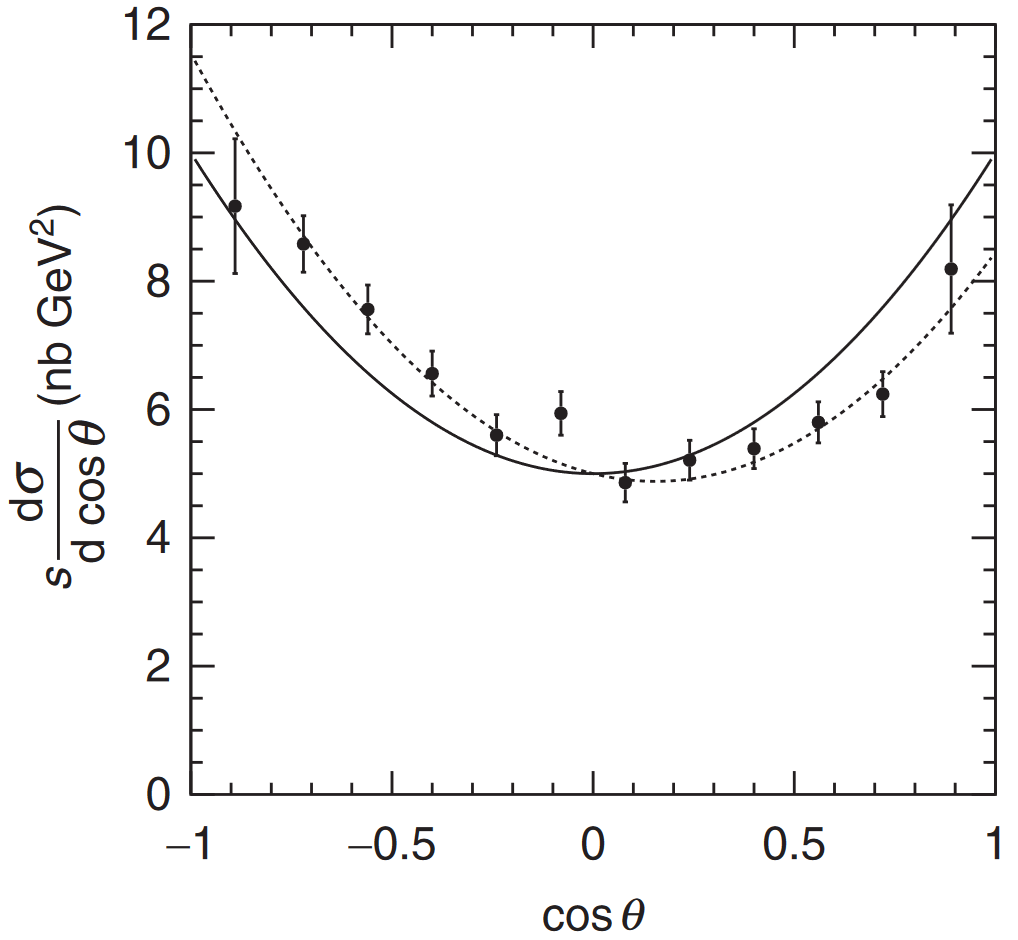
\includegraphics[width=0.8\textwidth]{images/electron-scattering-cross-section}
        \caption[Differential cross section for electron/positron scattering]{The differential cross section for the \(\Pe\APe \to \Pmu\APmu\) process. The line is the lowest order QED calculation, the dotted line includes electroweak interactions, and the data points are experimental measurements taken at \(\sqrt{s} = \qty{34.4}{\giga\electronvolt}\). Taken from \cite{thomson}, which adapted it from \cite{bartel}.}
    \end{figure}
    
    \subsection{Total Cross Section}
    We compute the total cross section by integrating the differential cross section.
    To do so consider the integral
    \begin{align}
        \int_{S^2} (1 + \cos^2\vartheta) \dd{\Omega} &= \int_{0}^{2\pi} \dl{\varphi} \int_{0}^{\pi} \dl{\vartheta} \, \sin\vartheta(1 + \cos^2\vartheta)\\
        &= 2\pi \int_{-1}^{1} (1 + \cos^2\vartheta) \dd{(\cos\vartheta)}\\
        &= \frac{16\pi}{3}.
    \end{align}
    We therefore have the total cross section to leading order in QED as
    \begin{equation}
        \sigma = \frac{4\pi\alpha^2}{3s}.
    \end{equation}
    This is very close to what we actually measure.
    
    \section{Invariant Form of the Amplitude}
    In the centre of mass frame the amplitude squared is
    \begin{equation}
        \abs{\amplitude}^2 = e^4(1 + \cos^2\vartheta).
    \end{equation}
    In the centre of mass frame the momenta of the particles are
    \begin{gather}
        p_1 = (E, 0, 0, E), \quad p_2 = (E, 0, 0, -E), \quad p_3 = (E, E\sin\vartheta, 0, E\cos\vartheta),\\
        \text{and} \quad p_4 = (E, -E\sin\vartheta, 0, -E\cos\vartheta).
    \end{gather}
    In the high energy limit, so \(E \gg m_{\symrm{e}}, m_{\text{μ}}\), we have \(s = 2E^2\), \(t = E^2(1 - \cos\vartheta)\), and \(t = E^2(1 + \cos\vartheta)\).
    We then have
    \begin{align}
        t^2 + u^2 &= E^4[(1 - \cos\vartheta)^2 + (1 + \cos\vartheta)^2]\\
        &= E^4[1 + \cos^2\vartheta - 2\cos\vartheta + 1 + \cos^2\vartheta + 2\cos\vartheta] \notag\\
        &= 2E^4(1 + \cos^2\vartheta).
    \end{align}
    Hence,
    \begin{equation}
        1 + \cos^2\vartheta = \frac{t^2 + u^2}{2E^4} = 2\frac{t^2 + u^2}{s^2}.
    \end{equation}
    So we can rewrite the amplitude squared as
    \begin{equation}
        \expected{\abs{\amplitude}^2} = 2e^4\frac{t^2 + u^2}{s^2}.
    \end{equation}
    This is written in terms of Lorentz invariants, and so is valid in any frame in the high energy limit.
    
    
    \chapter{Chirality}
    \section{\texorpdfstring{\(\Pe \APe \to \Pf \APf\)}{electron/positron to fermion/antifermion}}
    Consider the slightly more general process of an electron and positron annihilating and forming a photon, which decays into a charged fermion, \(\Pf\), and its antiparticle, \(\APf\).
    To first order this process occurs via the \(s\)-channel diagram
    \begin{equation}
        \tikzsetnextfilename{fd-electron-positron-to-fermion-antifermion}
        \feynmandiagram[horizontal=v1 to v2, inline=(v1)]{
            i1 [particle = \(\Pe\)] -- [fermion] v1 -- [photon] v2 -- [fermion] o1 [particle = \(\Pf\)],
            i2 [particle = \(\APe\)] -- [anti fermion] v1,
            v2 -- [anti fermion] o2 [particle = \(\APf\)]
        };
    \end{equation}
    Suppose that \(\Pf\) has charge \(-iQ_{\Pf}e\).
    Then the amplitude is
    \begin{equation}
        -i\amplitude = \diracadjoint{v}_{\symrm{e}}(p_2) ie\gamma^\mu u_{\symrm{e}}(p_1) \frac{-ig_{\mu\nu}}{q^2} \diracadjoint{u}_{\Pf}(p_3)(-iQ_{\Pf}e\gamma^\nu)v_{\Pf}(p_4) = \frac{Q_{\Pf}e^2}{s} j_{\symrm{e}} \cdot j_{\Pf}.
    \end{equation}
    The only difference from the muon case is the charge.
    
    For this process to be allowed we need \(\sqrt{s} \ge 2m_{\Pf}\).
    This is seen in experimental results where up to \(\sqrt{s} = 2m_{\Pf}\) the cross section for this process is zero.
    We can use this to measure the mass of the fermion, as shown in \cref{fig:threshold for tau}.
    
    \begin{figure}
        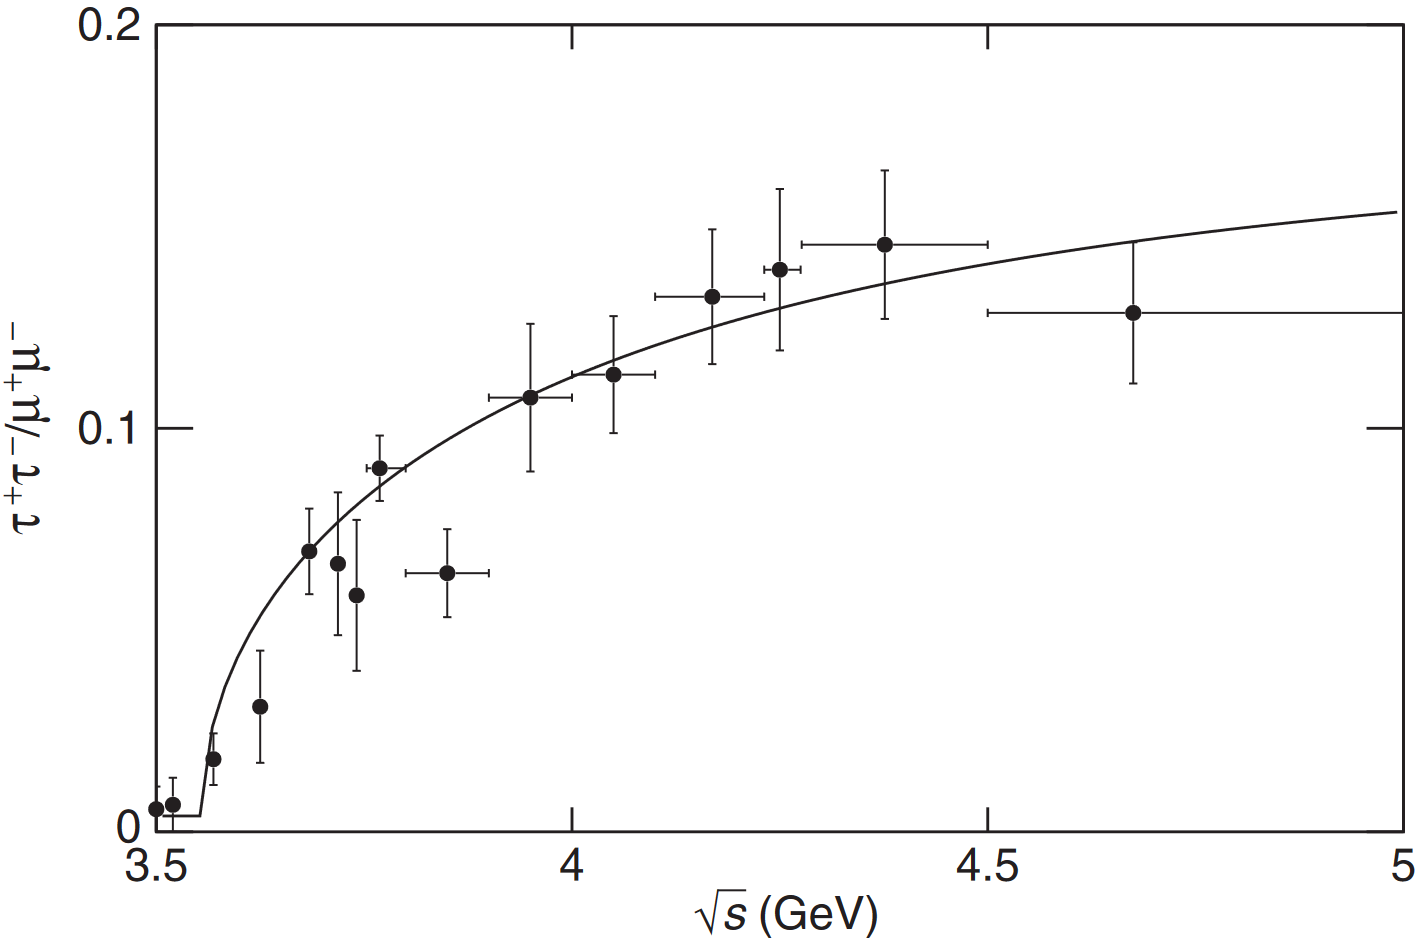
\includegraphics[width=0.8\textwidth]{images/tau-muon-cross-section-ratio-threshold}
        \caption[Threshold for producing tau particles.]{Plot showing the experimental measurements and theoretical predictions of the ratio \(\sigma(\Pe\APe \to \Ptau\APtau)/\sigma(\Pe\APe \to \Pmu\APmu)\). Notice that below about \qty{3.6}{\giga\electronvolt} this quantity vanishes. This corresponds to the tau particle having a mass of about \qty{1.8}{\giga\electronvolt}, so below this energy it is not possible to produce two tau particles. This figure was taken from \cite{thomson}, which modified it from \cite{bacino}.}
        \label{fig:threshold for tau}
    \end{figure}
    
    A full calculation, not just in the high energy level, gives the cross section for this process as
    \begin{equation}
        \sigma(\Pe\APe \to \Pf\APf) = \frac{4\pi\alpha^2Q_{\Pf}^2}{3s} \beta\left( \frac{3 - \beta^2}{2} \right).
    \end{equation}
    Here \(\beta = p_{3}/E_f = 1 - 4m_{\Pf}^2/s\) is the velocity of the fermion divided by the speed of light.
    
    
    \section{\texorpdfstring{\(\Pe\Pf \to \Pe\Pf\)}{Electron/Fermion Scattering}}
    Consider the related process of an electron and a charged fermion scattering.
    This can happen as a \(t\)-channel process,
    \begin{equation}
        \tikzsetnextfilename{fd-crossing-symmetry-example}
        \feynmandiagram[vertical = v1 to v2, small, baseline=(current bounding box)]{
            i1 [particle={\llap{\(p_1, \Pe\)}}] -- [fermion] v1 -- [fermion] o1 [particle={\rlap{\(\Pe, p_3\)}}],
            i2 [particle={\llap{\(p_2, \Pf\)}}] -- [fermion] v2 -- [fermion] o2 [particle={\rlap{\(\Pf, p_4\)}}],
            v1 -- [photon] v2
        };
    \end{equation}
    This is related to the \(\Pe\APe \to \Pf\APf\) process by \defineindex{crossing symmetry}.
    To see this consider the amplitude for this process:
    \begin{equation}
        -i\amplitude = \diracadjoint{u}_{\symrm{e}}(p_3) ie\gamma^\mu u_{\symrm{e}}(p_1) \frac{-i\gamma_{\mu\nu}}{q^2} \diracadjoint{u}_{\Pf}(p_4) (-iQ_{\Pf}e \gamma^\nu) u_{\Pf}(p_1) = \frac{Q_{\Pf}e^2}{t} j_{\symrm{e}} \cdot j_{\Pf}.
    \end{equation}
    Here \(q^2 = (p_1 - p_3)^2 = t\).
    The only difference is the momenta of the particles.
    If we make the substitution
    \begin{equation}
        p_1 \to p_1, \quad p_2 \to -p_3, \quad p_3 \to p_r, \qand p_4 \to -p_2
    \end{equation}
    in the amplitude for \(\Pe\APe \to \Pf\APf\) and swap antiparticles to be particles then we get the amplitude for \(\Pe\Pf \to \Pe\Pf\).
    This corresponds to swapping the Mandelstam invariants according to
    \begin{equation}
        s \to t, \qquad t \to u, \qand u \to s.
    \end{equation}
    So, the spin averaged amplitude squared is
    \begin{equation}
        \expected{\abs{\amplitude}^2} = 2Q_{\Pf}^2e^4 \frac{u^2 + s^2}{t^2}.
    \end{equation}
    
    \section{The Fifth Gamma Matrix}
    We now define the matrix
    \begin{equation}
        \gamma^5 \coloneqq i \gamma^0\gamma^1\gamma^2\gamma^3 = 
        \begin{pmatrix}
            0 & 0 & 1 & 0\\
            0 & 0 & 0 & 1\\
            1 & 0 & 0 & 0\\
            0 & 1 & 0 & 0
        \end{pmatrix}
        = 
        \begin{pmatrix}
            0 & \ident_2\\
            \ident_2 & 0
        \end{pmatrix}
        .
    \end{equation}
    This is a unitary matrix, \((\gamma^5)^\hermit \gamma^5 = 1\), and it anticommutes with all of the gamma matrices, \(\anticommutator{\gamma^5}{\gamma^\mu} = 0\).
    It is also Hermitian, \((\gamma^5)^\hermit = \gamma^5\), and so \((\gamma^5)^2 = 1\).
    
    \section{Chirality}
    Recall that helicity is defined as the spin along the direction of motion of the particle.
    This is determined in terms of the three-vector \(\vv{p}\), and so is \emph{not} Lorentz invariant.
    Instead we define a new quantity which is Lorentz invariant, called the \defineindex{chirality}, which is the eigenvalue of the fifth gamma matrix, \(\gamma^5\).
    
    Chirality turns out to be very important when it comes to which interactions can occur.
    Recall that, in the high energy limit, only four of the possible sixteen helicity combinations contributed a nonzero amount to the \(\Pe\APe \to \Pmu\APmu\) scattering amplitude.
    This turns out to be due to the fact that in the high energy limit, or equivalently, for massless particles, chirality and helicity are the same.
    This is because when \(m = 0\) the helicity operator commutes with the Hamiltonian, and is Lorentz invariant.
    The chiral structure of the electromagnetic interaction is then what restricts which helicity combinations contribute.
    
    Suppose that \(u_{\Right}\), \(u_{\Left}\), \(v_{\Right}\), and \(v_{\Left}\) are spinors which are eigenspinors of \(\gamma^5\), such that
    \begin{equation}
        \gamma^5 u_{\Right} = +u_{\Right}, \quad \gamma^5u_{\Left} = -u_{\Left}, \quad \gamma^5v_{\Right} = -v_{\Right}, \qand \gamma^5 v_{\Left} = +v_{\Left}.
    \end{equation}
    We call these right and left-handed \define{chiral spinors}\index{chiral spinor}.
    In the high energy/zero mass limit we find that \(u_{\Right} = u_{\uparrow}\), \(u_{\Left} = u_{\downarrow}\), \(v_{\Right} = v_{\uparrow}\), and \(v_{\Left} = v_{\downarrow}\).
    
    We define the \define{chiral projection operators}\index{chiral projection operator}
    \begin{equation}
        p_{\Right} \coloneqq \frac{1}{2}(1 + \gamma^5), \qqand P_{\Left} \coloneqq \frac{1}{2}(1 - \gamma^5).
    \end{equation}
    These project spinors as follows:
    \begin{itemize}
        \item \(P_{\Right}\) projects onto the right-handed chiral state of a particle,
        \item \(P_{\Right}\) projects onto the left-handed chiral state of an antiparticle,
        \item \(P_{\Left}\) projects onto the left-handed chiral state of a particle,
        \item \(P_{\Left}\) projects onto the right-handed chiral state of an antiparticle.
    \end{itemize}
    This can be shown by considering an arbitrary particle spinor, \(\alpha u_{\Right} + \beta u_{\Left}\), or an arbitrary antiparticle spinor, \(\alpha v_{\Right} + \beta v_{\Left}\), for \(\alpha, \beta \in \complex\).
    This works since the chiral spinors form a basis, so we can decompose an arbitrary spinor as
    \begin{equation}
        \psi = \psi_{\Left} + \psi_{\Right} = P_{\Left}\psi + P_{\Right}\psi.
    \end{equation}
    Another way of saying this is that \(\{P_{\Left}, P_{\Right}\}\) is a complete set of operators, so \(P_{\Left} + P_{\Right} = 1\).
    The chiral projectors are also orthogonal, so \(P_{\Right} P_{\Left} = P_{\Left}P_{\Right} = 0\).
    As projectors they are also idempotent, \(P_{\Right}^2 = P_{\Right}\) and \(P_{\Left}^2 = P_{\Left}\).
    
    Consider an arbitrary fermion current, \(j^\mu = \diracadjoint{\varphi} \gamma^\mu \psi\).
    We can write this as
    \begin{align}
        j^\mu &= (\diracadjoint{\varphi}_{\Left} + \diracadjoint{\varphi}_{\Right}) \gamma^\mu (\psi_{\Left} + \psi_{\Right})\\
        &= \diracadjoint{\varphi}_{\Left}\gamma^\mu \psi_{\Left} + \diracadjoint{\varphi}_{\Right} \gamma^\mu \psi_{\Right}.
    \end{align}
    Here we've used the fact that \(\diracadjoint{\varphi}_{\Left} \gamma^\mu \psi_{\Right} = \diracadjoint{\varphi}_{\Right} \gamma^\mu \psi_{\Left} = 0\).
    This shows that only certain combinations of chiral spinors contribute to the fermion current.
    This is why only certain helicity combinations don't vanish in our earlier calculation.
    
    QED treats left and right handed chiral spinors equally.
    The only important aspect of chirality when it comes to QED is this cancelling of mixed chirality components.
    If we were to swap all left chiral spinors for right chiral spinors, and vice versa, nothing would change as far as QED is concerned.
    In terms of the \(\Pe\APe \to \Pmu\APmu\) process the chiral structure means that we don't produce muons with physically unaligned spins.
    Since the muons go in opposite directions this means we produce one left-handed muon and one right-handed antimuon, or vice versa.
    Conservation of angular momentum then requires that we have a left-handed electron and right-handed positron, or vice versa.
    
    \chapter{Symmetries}
    \section{Parity}
    Parity is the operation
    \begin{gather}
        x^\mu = (t, \vv{x}) \mapsto x'^\mu = \parity x^\mu = (t, -\vv{x}), \qquad \text{or}\\
        t \mapsto t' = \parity t = t, \qqand \vv{x} \mapsto \vv{x}' = \parity \vv{x} = -\vv{x}.
    \end{gather}
    That is, parity inverts space, and leaves time unaffected.
    Parity acts on the wave function according to
    \begin{equation}
        \psi \mapsto \psi'(t', \vv{x}') = \parity\psi(\parity t, \parity\vv{x}) = \psi(t, -\vv{x}).
    \end{equation}
    Inverting space and then inverting it again gets us back to where we started, so we have \(\parity^2 = 1\).
    
    Consider the Dirac equation, and some spinor, \(\psi\), satisfying it.
    Then, by definition
    \begin{equation}
        (i\slashed{\partial} - m)\psi = 0.
    \end{equation}
    Let \(\psi' = \parity \psi\).
    Under parity \(\psi_i \mapsto -\partial_i\), and \(\partial_0 \mapsto \partial_0\).
    So, the Dirac equation becomes
    \begin{equation}
        i\gamma^0 \partial_0 \psi - i\vv{\gamma} \cdot \grad \psi - m\psi = 0.
    \end{equation}
    Multiply through by \(\gamma^0\), and we have
    \begin{equation}
        i(\gamma^0)^2 \partial_0 \psi - i\gamma^0\vv{\gamma} \cdot \grad \psi - m\gamma^0\psi = 0.
    \end{equation}
    Now using \((\gamma^0)^2 = 0\) and \(\gamma^0 \gamma^i = -\gamma^i \gamma^0\) we have
    \begin{equation}
        i\partial_0\psi + i\gamma^i\gamma^0 \partial_i \psi - m\gamma^0\psi = 0.
    \end{equation}
    We can now replace \(\psi\) with \(\parity \psi'\), and so we have
    \begin{equation}
        i\parity \partial_0 \psi' + i\gamma^i\gamma^0 \parity \partial_i \psi' - m\gamma^0 \parity \psi = 0.
    \end{equation}
    We expect that \(\psi'\) satisfies the Dirac equation in it's own frame, so
    \begin{equation}
        i\gamma^0\partial_0 \psi' + i\gamma^i \partial_i \psi' - m\psi' = 0.
    \end{equation}
    Comparing these two equations we see that we must have \(\gamma^0 \parity \propto 1\).
    Since \(\parity^2 = 1\) we can choose \(\parity = \gamma^0\).
    So, for spinors, we have
    \begin{equation}
        \psi' = \parity\psi = \gamma^0\psi.
    \end{equation}
    There is actually some ambiguity in the sign, we could also have chosen \(\parity = -\gamma^0\), or in fact \(\parity = \e^{i\vartheta} \gamma^0\) for some \(\vartheta \in \reals\).
    
    If we apply \(\parity = \pm\gamma^0\) to the spinors in the rest frame then we find that
    \begin{equation}
        \parity u_1 = \pm u_1, \quad \parity u_2 = \pm u_2, \quad \parity v_1 = \mp \parity v_1, \qand \parity v_2 = \mp \parity v_2.
    \end{equation}
    We are free to choose the sign, and the conventional choice is that we choose \(\parity = +\gamma^0\), so
    \begin{itemize}
        \item the intrinsic parity quantum number of fundamental spin \(1/2\) particles is positive,
        \item the intrinsic parity quantum number of fundamental spin \(1/2\) antiparticles is negative.
    \end{itemize}
    
    Under parity \(\vv{x} \mapsto -\vv{x}\), and \(\vv{p} \mapsto -\vv{p}\).
    So,
    \begin{equation}
        \vv{S} = \vv{x} \times \vv{p} \mapsto (-\vv{x}) \times (-\vv{p}) = \vv{x} \times \vv{p} = \vv{S}.
    \end{equation}
    This means the direction of spin doesn't change under parity.
    We say that spin is an axial or pseudovector.
    The result is that helicity, which is spin in the \(\vv{p}\) direction, flips under parity transformations.
    So parity transforms right-handed states into left-handed states and vice versa.
    This corresponds to the gamma matrices identity \(\gamma^0\gamma^5 = -\gamma^5\gamma^0\).
    
    \section{Charge Conjugation}
    Consider an electron in an electromagnetic field.
    This is described by the modified Dirac equation
    \begin{equation}
        (i\slashed{\partial} - q\slashed{A} - m)\psi = 0.
    \end{equation}
    For an electron with charge \(q = -e\) we then have
    \begin{equation}
        (i\slashed{\partial} + e\slashed{A} - m)\psi = 0.
    \end{equation}
    For a positron, with charge \(q = e\) we instead have
    \begin{equation}
        (i\slashed{\partial} - e\slashed{A} - m)\psi = 0.
    \end{equation}
    Take the complex conjugate of this, and we get
    \begin{equation}
        (-i\slashed{\partial}^* - e\slashed{A}^* - m)\psi^* = 0.
    \end{equation}
    Multiply through by \(\gamma^2\) and we get
    \begin{equation}
        (-i\gamma^2\slashed{\partial}^* - e\gamma^2\slashed{A}^* - m\gamma^2)\psi^* = 0.
    \end{equation}
    Now use \((\gamma^2)^* = -\gamma^2\) we have \(\gamma^2(\gamma^2)^* = -(\gamma^2)^2\) and \(\gamma^2(\gamma^\mu)^* = \gamma^2\gamma^\mu = -\gamma^\mu\gamma^2\) for \(\mu \ne 2\), since \((\gamma^\mu)^* = \gamma^\mu\) for \(\mu \ne 2\) and \(\gamma^\mu\) anticommutes with \(\gamma^2\) for \(\mu \ne 2\).
    We then have
    \begin{align}
        (-i\slashed{\partial}\gamma^2 - e\slashed{A}\gamma^2 - m\gamma^2)\psi^* &= 0,\\
        (-i\slashed{\partial} + e\slashed{A} - m)\gamma^2\psi^* &= 0,\\
        (\slashed{\partial} + ie\slashed{A} + im)\psi' &= 0,
    \end{align}
    where \(\psi' = i\gamma^2\psi'\).
    We interpret this as \(\psi'\) describing another spin \(1/2\) particle with the same mass but opposite charge.
    
    We call the operation
    \begin{equation}
        \psi \mapsto \psi' = \chargeConjugation \psi = i\gamma^2\psi^*
    \end{equation}
    \defineindex{charge conjugation}.
    By considering specific cases we can show that this maps particles to antiparticles and vice versa, and hence maps positive charge to negative charge and vice versa.
    For example, consider \(\psi = u_1 \exp[-ip \cdot x]\).
    Under charge conjugation \(u_1\) mapsto
    \begin{equation}
        i\gamma^1u_1^* = i\sqrt{E + m}
        \begin{pmatrix}
            0 & 0 & 0 & -i \\
            0 & 0 & i & 0 \\
            0 & i & 0 & 0 \\
            -i & 0 & 0 & 0
        \end{pmatrix}
        \begin{pmatrix}
            1\\ 0\\ \frac{p_z}{E + m}\\ \frac{p_x + ip_y}{E + m}
        \end{pmatrix}
        ^* = \sqrt{E + m}
        \begin{pmatrix}
            \frac{p_x - ip_y}{E + m}\\ \frac{-p_z}{E + m}\\ 0\\ 1
        \end{pmatrix}
        = v_1,
    \end{equation}
    and so
    \begin{equation}
        \psi = u_1 \e^{-ip \cdot x} \mapsto v_1 \e^{+ip \cdot x}.
    \end{equation}
    
    Charge conjugation is such that \(\chargeConjugation^2 = 1\), swapping matter and antimatter twice gets us back to where we started.
    
    \section{Time Reversal}
    Time reversal changes the direction of time, so
    \begin{equation}
        x^\mu = (t, \vv{x}) \mapsto x'^\mu = \timeReversal x^\mu = (-t, \vv{x}).
    \end{equation}
    Since the direction of time reverses we have \(\partial_0 \mapsto -\partial_0\), and so \(\vv{p} \mapsto -\vv{p}\).
    However, \(\vv{x}\) is unchanged, so \(\vv{S} \mapsto -\vv{S}\).
    Hence, helicity is flipped by time reversal.
    
    Experimentally it is much harder to reverse time than it is to either use antiparticles or do the experiment in the opposite direction.
    It is also theorised that the combined symmetry \(\chargeConjugation\parity\timeReversal\) is a symmetry of all systems, and if this is the case then \(\timeReversal\) is necessarily equivalent to \(\chargeConjugation\parity\).
    So, we often talk about charge conjugation and parity in place of time reversal.
    
    Time reversal is such that \(\timeReversal^2 = 1\).
    It can be shown that  we can represent time reversal on spinors as \(\timeReversal = i\gamma^1\gamma^3\).
    
    \section{Gauge Symmetry}
    \subsection{Classical Electrodynamics}
    \begin{rmk}
        See \course{Classical Electrodynamics} for details in the covariant formulation and \course{Electromagnetism} for details in the noncovariant formalism.
    \end{rmk}
    Consider the electric and magnetic fields defined in terms of the potentials:
    \begin{equation}
        \vv{E} = -\grad\varphi - \diffp{\vv{A}}{t}, \qqand \vv{B} = \curl \vv{A}.
    \end{equation}
    Alternatively, in a covariant notation
    \begin{equation}
        F^{\mu\nu} = \partial^\mu A^\nu - \partial^\nu A^\mu
    \end{equation}
    where \(A^\mu = (\varphi, \vv{A})\).
    
    Now consider the transformation \(\varphi \mapsto \varphi - \partial_t\chi\) and \(\vv{A} \mapsto \vv{A} + \grad\chi\), where \(\chi\) is some scalar field with everywhere continuous second derivatives.
    Then
    \begin{equation}
        \vv{E} \mapsto -\grad\varphi - \grad(\partial_t \chi) - \partial_t\vv{A} - \partial_t(\grad \chi) = -\grad\varphi - \partial_t\vv{A} = \vv{E}
    \end{equation}
    and
    \begin{equation}
        \vv{B} \mapsto \curl\vv{A} + \curl(\grad\chi) = \curl\vv{A} = \vv{B}.
    \end{equation}
    So the physics doesn't change under this transformation of the potentials.
    We call a transformation like this a \defineindex{gauge transformation}.
    
    In covariant notation this gauge transformation is \(A_\mu \mapsto A_\mu - \partial_\mu \chi\).
    We then have
    \begin{align}
        F_{\mu\nu} &\mapsto \partial_\mu(A_\nu - \partial_\nu \chi) - \partial_\nu(A_\mu - \partial_\mu \chi)\\
        &= \partial_\mu A_\nu - \partial_\nu A_\mu - \partial_\mu \partial_\nu \chi + \partial_\nu \partial_\mu \chi\\
        &= \partial_\mu A_\nu - \partial_\nu A_\mu\\
        &= F_{\mu\nu}.
    \end{align}
    So, we see exactly the same invariance under a gauge transformation.
    
    \subsection{Local \texorpdfstring{\(\unitary(1)\)}{U(1)} Gauge Transformation}
    Suppose that we transform the state by some phase depending on the charge and some scalar field, \(\chi\), with everywhere continuous second derivatives:
    \begin{equation}
        \psi \mapsto \psi' = \e^{iq\chi}\psi.
    \end{equation}
    This is called a \(\unitary(1)\) symmetry, where
    \begin{equation}
        \unitary(1) \coloneqq \{\e^{i\varphi} \in \complex \mid \varphi \in [0, 2\pi)\} \cong S^1
    \end{equation}
    is the unitary group in one dimension, and is the group of symmetries of the circle\footnote{for details see \course{Symmetries of Quantum Mechanics} or \course{Symmetries of Particles and Fields}}.
    
    Consider the Dirac equation for this transformed field:
    \begin{equation}
        (i\slashed{\partial} - m)\psi = 0 \mapsto i\slashed{\partial}(\psi\e^{iq\chi}) - m\psi\e^{iq\chi} = 0.
    \end{equation}
    Taking the derivative we get
    \begin{equation}
        i(\slashed{\partial}\psi)\e^{iq\chi} + i\psi(iq\slashed{\partial}\chi)\e^{iq\chi} - m\e^{iq\chi} = 0.
    \end{equation}
    Hence, we have
    \begin{equation}
        i(\slashed{\partial} + iq\slashed{\partial}\chi)\psi - m\psi = 0.
    \end{equation}
    
    Suppose that at the same time as we transform the spinor we also modify the derivative \(\partial_\mu \mapsto \partial_\mu + iq A_\mu\) where \(A_\mu\) transforms under this transformation as \(A_\mu \mapsto A_\mu - \partial_\mu \chi\).
    Then we instead have the modified Dirac equation
    \begin{equation}
        i(\slashed{\partial} + iq\slashed{A})\psi - m\psi = 0.
    \end{equation}
    The modified derivative then transforms as
    \begin{equation}
        \slashed{\partial} + iq\slashed{A} \mapsto \slashed{\partial} + iq\slashed{A} - iq\slashed{\partial}\chi.
    \end{equation}
    So, we see that under these transformations the Dirac equation transforms as
    \begin{align}
        0 = i(\slashed{\partial} + iq\slashed{A})\psi - m\psi &\mapsto i(\slashed{\partial} + iq\slashed{A} - iq\slashed{\partial}\chi + iq\slashed{\partial}\chi) - m\psi\\
        &= i(\slashed{\partial} + iq\slashed{A})\psi - m\psi = 0.
    \end{align}
    So, the modified Dirac equation is invariant under this \(\unitary(1)\) symmetry.
    
    Note that we can write the modified Dirac equation as
    \begin{equation}
        (i\slashed{D} - m)\psi = 0
    \end{equation}
    where
    \begin{equation}
        D_\mu = \partial_\mu + iqA_\mu
    \end{equation}
    is the \defineindex{gauge covariant derivative}\footnote{see \course{General Relativity} for another use of covariant derivatives, where the gauge symmetry is invariance under diffeomorphisms.}
    
    If we interpret \(A_\mu\) as the photon field then we see that demanding \(\unitary(1)\) symmetry invariance automatically implies the existence of photons and much of electrodynamics.
    Formally, we say that QED is an Abelian gauge theory with an \(\unitary(1)\) symmetry group.
    
    \part{QCD}    
    \chapter{Quantum Chromodynamics}
    \section{Comparison to QED}
    \define{Quantum chromodynamics}\index{quantum chromodynamics}, or QCD, is the quantum field theory of the strong force.
    Formally, QCD is a non-Abelian gauge theory with \(\specialUnitary(3)\) symmetry group.
    We'll see what this means shortly.
    First, we make some comparisons between QCD and QED.
    
    \begin{multiitem}
        \mitemxx{QED}{QCD}
        \mitemxx{Charged particles carry electric charge.}{Quarks carry colour charge.}
        \mitemxx{Electric charge has a single degree of freedom.}{Colour charge has three degrees of freedom. We call them red, green, and blue, or \(\Pred\), \(\Pgreen\), \(\Pblue\).}
        \mitemxx{Antiparticles have the opposite electric charge.}{Antiquarks have anticolour charge, \(\APred\), \(\APgreen\), or \(\APblue\).}
        \mitemxx{Force is mediated by massless spin 1 photons.}{Force is mediated by massless spin 1 gluons.}
        \mitemxx{The strength is dictated by the value of \(e = \sqrt{\alpha/(4\pi)}\).}{The strength is dictated by the value of \(g_{\strongForce} = \sqrt{\alpha_{\strongForce}/(4\pi)}\).}
        \mitemxx{\(\alpha \approx 1/137\)}{\(\alpha_{\strongForce} \approx 1\).}
        \mitemxx{\(\unitary(1)\) gauge theory.}{\(\specialUnitary(3)\) gauge theory.}
    \end{multiitem}
    
    \section{QCD Gauge Theory}
    \begin{rmk}
        The group theory gets a bit complex here.
        I've included the simple definitions given in lectures, and more complicated, nonexaminable points in \textit{italics}.
        See \course{Symmetries of Quantum Mechanics} and \course{Symmetries of Particles and Fields} for more details.
    \end{rmk}
    QCD treats all three colours the same.
    This means we can mix the colours and the state only changes up to an unobservable phase.
    The symmetry group which does this mixing is \(\specialUnitary(3)\), where
    \begin{equation}
        \specialUnitary(3) \coloneqq \{U \in \matrices{3}{\complex} \mid U^\hermit U = 1 \text{ and } \det U = 1\}
    \end{equation}
    is the special unitary group of \(3 \times 3\) matrices.
    Note that the special part corresponds to the \(\det U = 1\) requirement, and the unitary part to the \(U^\hermit U = 1\) requirement.
    \textit{\(\specialUnitary(3)\) is the symmetry group preserving the inner product \(\langle x, y\rangle  = x_i^* y_i\) on \(\complex^3\), this is one particular representation of it.}
    
    In QED the symmetry group \(\unitary(1)\) has one possible transformation, a phase factor, \(e^{iq\chi}\).
    \textit{In QED the symmetry group \(\unitary(1)\) has the Lie algebra \(\unitaryLie(1)\), which has a single generator, \(q\chi\).}
    This corresponds to a single field, \(A_\mu\), in QED, and so a single exchange particle.
    In QCD the symmetry group \(\specialUnitary(3)\) has eight possible transformations, \(T_a = \lambda_a/2\), where \(a = 1, \dotsc, 8\) and
    \begin{align}
        \lambda^1 &= 
        \begin{pmatrix}
            0 & 1 & 0\\
            1 & 0 & 0\\
            0 & 0 & 0
        \end{pmatrix}
        ,\qquad & \lambda^2 &= 
        \begin{pmatrix}
            0 & -i & 0\\
            i & 0 & 0\\
            0 & 0 & 0
        \end{pmatrix}
        ,\qquad & \lambda^3 &= 
        \begin{pmatrix}
            1 & 0 & 0\\
            0 & -1 & 0\\
            0 & 0 & 0
        \end{pmatrix}
        ,\notag\\
        \lambda^4 &= 
        \begin{pmatrix}
            0 & 0 & 1\\
            0 & 0 & 0\\
            1 & 0 & 0
        \end{pmatrix}
        ,\qquad & \lambda^5 &= 
        \begin{pmatrix}
            0 & 0 & -i\\
            0 & 0 & 0\\
            i & 0 & 0
        \end{pmatrix}
        ,\qquad & \lambda^6 &= 
        \begin{pmatrix}
            0 & 0 & 0\\
            0 & 0 & 1\\
            0 & 1 & 0
        \end{pmatrix}
        ,\notag\\
        \lambda^7 &= 
        \begin{pmatrix}
            0 & 0 & 0\\
            0 & 0 & -i\\
            0 & i & 0
        \end{pmatrix}
        ,\qquad & \lambda^8 &= \frac{1}{\sqrt{3}}
        \begin{pmatrix}
            1 & 0 & 0\\
            0 & 1 & 0\\
            0 & 0 & -2
        \end{pmatrix}
        .
    \end{align}
    These are called the \defineindex{Gell-Mann matrices}.
    \textit{In QCD the symmetry group \(\specialUnitary(3)\) has the Lie algebra \(\specialUnitaryLie(3)\), which has eight generators, \(T_a\). The fundamental representation of this Lie algebra consists of \(3\times 3\) complex traceless Hermitian matrices, \(M\), such that \(\exp[iM] \in \specialUnitary(3)\). In this representation one choice is \(T_a = \lambda_a/2\). We can then express an arbitrary element of \(\specialUnitaryLie(3)\) as \(\alpha^aT_a\) and so an arbitrary element of \(\specialUnitary(3)\) can be expressed as \(\exp[i\strongCoupling\alpha^aT_a]\).}
    A general gauge transformation of the spinor field is then
    \begin{equation}
        \psi \mapsto \psi' = \e^{i\strongCoupling \alpha^aT_a} \psi
    \end{equation}
    where \(\strongCoupling\) is a constant corresponding to the strength of the strong force, \(\alpha^a\) is a set of parameters and \(T_a = \lambda_a/2\) are the matrices defined above.
    \textit{This product here, between \(\exp[i\strongCoupling \alpha^a T_\alpha]\) and \(\psi\), is a tensor product, between these terms, since \(\psi\) above is a four-component spinor and \(\exp[i\strongCoupling\alpha^aT_a]\) is a \(3\times 3\) matrix there is no way to actually compute this as a matrix product, its just a formal statement that we have two components now to our wave function, a spinor, \(\psi\), and a colour phase, \(\exp[i\strongCoupling\alpha^aT_a]\). Note that \(\specialUnitaryLie(3)\) is a semisimple Lie algebra, and so it's Killing form is proportional to the identity. This means we don't need to distinguish raised and lowered indices, and sometimes we won't, but we do here as it makes the use of the summation convention more obvious.}
    
    The eight generators correspond to there being eight gluons.
    For each gluon, indexed by \(a = 1, \dotsc, 8\), we introduce a gluon field, \(G^a_\mu\), which corresponds to \(A_\mu\) in QED.
    Like photons these \(G^a_\mu\) fields correspond to massless exchange particles, and we have to modify the Dirac equation as we did for QED, changing the derivative to be
    \begin{equation}
        \partial_\mu \mapsto D_\mu = \partial_\mu + i\strongCoupling G^a_\mu T_a,
    \end{equation}
    and so the Dirac equation becomes
    \begin{equation}
        i(\slashed{\partial} + i\strongCoupling\slashed{G}^aT_a)\psi - m\psi = 0.
    \end{equation}
    
    To go from QED to QCD we replace \(q\chi\) with \(\strongCoupling T_a\), and \(A_\mu\) with \(G_\mu^a\).
    Thus, in a QCD interaction we replace the vertex term \(-iQ_{\Pf}e\gamma^\mu\) with
    \begin{equation}
        -\strongCoupling \gamma^\mu T_a.
    \end{equation}
    
    In order to do QCD we need to include a colour factor in our spinors.
    We do so by replacing \(u(p)\) with \(u_j(p) = c_iu(p)\), where
    \begin{equation}
        c_1 = \Pred = 
        \begin{pmatrix}
            1\\ 0\\ 0
        \end{pmatrix}
        , \qquad c_2 = \Pgreen = 
        \begin{pmatrix}
            0\\ 1\\ 0
        \end{pmatrix}
        , \qqand c_3 = \Pblue =
        \begin{pmatrix}
            0\\ 0\\ 1
        \end{pmatrix}
        .
    \end{equation}
    Again, this is just a formal product \textit{i.e., element of tensor product between two Hilbert spaces, one three dimensional colour space and one four dimensional spinor space}, there's no way to actually compute it as a matrix product.
    We assume that in this formal product all colour terms commute with all spinor terms \textit{which is exactly true for a tensor product in the sense that we can factor out the colour and spinor parts (there's no entangled states here)}.
    
    The QCD quark current corresponding to the vertex
    \begin{equation}
        \tikzsetnextfilename{fd-QCD-vertex}
        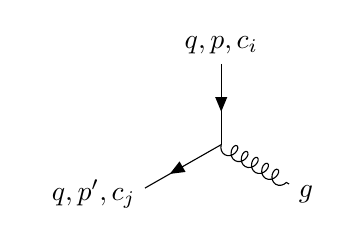
\begin{tikzpicture}
            \begin{feynman}
                \diagram[small]{
                    i1 [particle={\(\Pq, p, c_i\)}] -- [fermion] v,
                    i2 [particle={\llap{\(\APq, p', c_j\)}}] -- [anti fermion] v,
                    v -- [gluon] i3 [particle=\Pg]
                };
            \end{feynman}
            \node[left=of i2] {};
        \end{tikzpicture}
    \end{equation}
    is given by making the relevant substitutions to the QED fermion current:
    \begin{align}
        j^\mu &= \diracadjoint{u}(p') c_j^\hermit \left( -\frac{1}{2}i\strongCoupling \lambda_a \gamma^\mu \right) c_i u(p)\\
        &= -\frac{1}{2}i\strongCoupling c_j^\hermit \lambda_a c_i \diracadjoint{u}(p')\gamma^\mu u(p)\\
        &= -\frac{1}{2}i\strongCoupling (\lambda_a)_{ji} \diracadjoint{u}(p')\gamma^\mu u(p).
    \end{align}
    Here \((\lambda_a)_{ji}\) is the entry of the \(j\)th row and \(i\)th column of \(\lambda_a\).
    
    Colour is conserved.
    This means if we have an internal gluon then the colour at one end must be the same as the colour at the other end.
    To enforce this we include a factor of \(\delta^{ab}\) for each internal gluon.
    
    \section{Feynman Rules}
    The Feynman rules for QCD are very similar to the Feynman rules for QED.
    For each external quark of momentum \(p\) we have
    \begin{equation}
        \begin{array}{rrr}
            \text{Incoming quark} & u(p) & \tikzsetnextfilename{fd-incoming-quark}\feynmandiagram[horizontal=a to b]{a -- [fermion] b [dot]}; \\
            \text{Outgoing quark} & \diracadjoint{u}(p) & \tikzsetnextfilename{fd-outgoing-quark}\feynmandiagram[horizontal=a to b]{a [dot] -- [fermion] b}; \\
            \text{Incoming antiquark} & \diracadjoint{v}(p) & \tikzsetnextfilename{fd-incoming-antiquark}\feynmandiagram[horizontal=a to b]{a -- [anti fermion] b [dot]}; \\
            \text{Outgoing antiquark} & v(p) & \tikzsetnextfilename{fd-outgoing-antiquark}\feynmandiagram[horizontal=a to b]{a [dot] -- [anti fermion] b};
        \end{array}
    \end{equation}
    Next, we have the rules for spin 1 external particles, which in QCD are just gluons.
    For a gluon with momentum \(p\) we have
    \begin{equation}
        \begin{array}{rlr}
            \text{Incoming gluon} & \varepsilon^\mu(p) & \tikzsetnextfilename{fd-incoming-gluon}\feynmandiagram[horizontal=a to b]{a -- [gluon] b [dot]}; \, \mu, a \\
            \text{Outgoing gluon} & \varepsilon^\mu(p)^* & \mu, a \, \tikzsetnextfilename{fd-outgoing-gluon}\feynmandiagram[horizontal=a to b]{a [dot] -- [gluon] b};
        \end{array}
    \end{equation}
    Then there are internal lines, for an internal gluon of momentum \(q\):
    \begin{equation}
        \begin{array}{rrr}
            \text{Gluon propagator} & \displaystyle-\frac{i\minkowskiMetric_{\mu\nu}}{q^2}\delta^{ab} & \mu, a \, \tikzsetnextfilename{fd-internal-gluon}\feynmandiagram[horizontal=a to b]{a [dot] -- [gluon] b [dot]}; \, \nu, b
        \end{array}
    \end{equation}
    Then there is a vertex factor of
    \begin{equation}
        -i\frac{1}{2}\strongCoupling (\lambda_a)_{ji}\gamma^\mu
    \end{equation}
    where \(c_j\) is the colour of the incoming quark and \(c_i\) the colour of the outgoing quark.
    
    \section{Quark-Antiquark Scattering}
    Consider the process of a quark and antiquark scattering.
    The diagram for this is
    \begin{equation}
        \tikzsetnextfilename{fd-quark-antiquark-scattering}
        \feynmandiagram[small, baseline=(current bounding box), vertical=v1 to v2]{
            i1 [particle=\Pq] -- [fermion, edge label'=\(i\)] v1 -- [fermion, edge label'=\(j\)] o1 [particle=\Pq],
            i2 [particle=\APq] -- [anti fermion, edge label=\(k\)] v2 -- [anti fermion, edge label=\(l\)] o2 [particle=\APq],
            v1 -- [gluon] v2
        };
    \end{equation}
    The amplitude for this is given by
    \begin{equation}
        -i\amplitude = \left[ \diracadjoint{u}_j \left( -i\frac{1}{2}\strongCoupling (\lambda_a)_{ji} \gamma^\mu u_i \right) \right] \frac{-i\minkowskiMetric_{\mu\nu}}{q^2} \delta^{ab} \left[ \diracadjoint{v}_k \left( -i\frac{1}{2}\strongCoupling (\lambda_b)_{kl} \gamma^\nu \right) v_l \right],
    \end{equation}
    which simplifies to
    \begin{equation}
        \amplitude = -\frac{1}{4} \strongCoupling^2 (\lambda_a)_{ji}(\lambda_a)_{kl} \frac{\minkowskiMetric_{\mu\nu}}{q^2} \diracadjoint{u}_j \gamma^\mu u_i \diracadjoint{v}_k \gamma^\nu v_l.
    \end{equation}
    Here we use the \(\delta^{ab}\) to change \(b\) into \(a\).
    
    \section{Colour Factors}
    Notice how similar this is to electron/positron scattering, but with \(e\) swapped for \(\strongCoupling\) and an extra factor of \((\lambda_a)_{ji}(\lambda^a)_{kl}/4\).
    This suggests that, to lowest order, we can approximate the dynamics of the \(\Pq\APq \to \Pq\APq\) scattering process as occurring in a Coulomb-like potential:
    \begin{equation}
        V_{\Pq\APq} = -\frac{f\alpha_{\strongForce}}{r} \qqwhere f = \frac{1}{4}(\lambda_a)_{ji}(\lambda_a)_{kl}.
    \end{equation}
    We call \(f\) the \defineindex{colour factor}.
    Note that \(a\) is summed over whereas \(i\), \(j\), \(k\) and \(l\) are fixed by the colour of the quarks.
    As with electron helicities we assume that the initial (anti)colour is an equal mix of all three colours, so we average over initial (anti)colours, and we assume the final (anti)colour isn't measured and sum over final (anti)colours.
    
    We can fairly easily, if not a bit laboriously, compute the value of the colour factor for a given interaction.
    We'll consider the \(\Pq\APq \to \Pq\APq\) scattering above.
    One point which allows for more efficient calculations is that QCD is symmetric under exchanging of colours, so if, for example, we compute all colour factors going from \(\Pred\APred\) to any other colour combination we know that the value of the colour factors from \(\Pgreen\APgreen\) to any other colour factor will be the same if we just exchange \(\Pred\) and \(\Pgreen\) as well as \(\APred\) and \(\APgreen\).
    
    Up to this rotation of colours there are three possible colour options for \(\Pq\APq \to \Pq\APq\) scattering.
    First, we could start with \(\Pred\APred\), choosing red arbitrarily, colour is conserved in QCD, so since this initial state is colour neutral we must end with a colour neutral state.
    First, its possible to have no colour change, so our final state would be \(\Pred\APred\).
    Second, we could have both quarks change colour, but we still need to be colour neutral.
    This would correspond to a final state of \(\Pg\APg\), again choosing green arbitrarily as colour which is not red.
    The only other colour combination we could start with is different colours and anticolours, say \(\Pred\Pgreen\), and then in order to conserve colour we can't have a change in colour, so we'd have the final state \(\Pred\Pgreen\) as well.
    
    The colour factors can then be computed.
    First consider \(\Pred\APred \to \Pred\APred\), this corresponds to \(i = j = k = l = 1\).
    The only Gell-Mann matrices which aren't zero in the first row and first column are \(\lambda^3\) and \(\lambda^8\), having values \(1\) and \(1/\sqrt{3}\) in this position respectively.
    The colour factor is then
    \begin{align}
        f_{\Pred\APred \to \Pred\APred} &= \frac{1}{4}(\lambda_a)_{11}(\lambda_a)_{11}\\
        &= \frac{1}{4} (\lambda_{11}^3\lambda_{11}^3 + \lambda_{11}^8\lambda_{11}^8)\\
        &= \frac{1}{4}\left( 1 \cdot 1 + \frac{1}{\sqrt{3}} \cdot \frac{1}{\sqrt{3}} \right)\\
        &= \frac{1}{3}.
    \end{align}
    By symmetry we then also have
    \begin{equation}
        f_{\Pgreen\APgreen \to \Pgreen\APgreen} = f_{\Pblue\APblue \to \Pblue\APblue} = f_{\Pred\APred \to \Pred\APred} = \frac{1}{3}.
    \end{equation}
    
    Similarly, for \(\Pred\APred \to \Pgreen\APgreen\) we have \(i = k = 1\) and \(j = l = 2\), giving
    \begin{align}
        f_{\Pred\APred \to \Pgreen\APgreen} &= \frac{1}{4}(\lambda_a)_{21}(\lambda_a)_{12}\\
        &= \frac{1}{4}(\lambda_{21}^1\lambda_{12}^1 + \lambda_{21}^2\lambda_{12}^2)\\
        &= \frac{1}{4}(1 \cdot 1 + i \cdot (-i))\\
        &= \frac{1}{2}
    \end{align}
    and by symmetry
    \begin{equation}
        f_{\Pred\APred \to \Pblue\APblue} = f_{\Pgreen\APgreen \to \Pred\APred} = f_{\Pgreen\APgreen \to \Pblue\APblue} = f_{\Pblue\APblue \to \Pred\APred} = f_{\Pblue\APblue \to \Pgreen\APgreen} = f_{\Pred\APred \to \Pgreen\APgreen} = \frac{1}{2}.
    \end{equation}
    Finally, for \(\Pred\APgreen \to \Pred\APgreen\) we have \(i = j = 1\) and \(k = l = 2\), so
    \begin{align}
        f_{\Pred\APgreen \to \Pred\APgreen} &= \frac{1}{4}(\lambda_a)_{22}(\lambda_a)_{11}\\
        &= \frac{1}{4}(\lambda^3_{22}\lambda^3_{11} + \lambda^8_{22}\lambda^8_{11})\\
        &= \frac{1}{4}\left( (-1) \cdot 1 + \frac{1}{\sqrt{3}} \cdot \frac{1}{\sqrt{3}} \right)\\
        &= -\frac{1}{6}.
    \end{align}
    By symmetry we then have
    \begin{equation}
        f_{\Pgreen\APred \to \Pgreen\APred} = f_{\Pgreen\APblue \to \Pgreen\APblue} = f_{\Pblue\APred \to \Pblue\APred} = f_{\Pblue\APgreen \to \Pblue\APgreen} = f_{\Pred\APblue \to \Pred\APblue} = f_{\Pred\APgreen \to \Pred\APgreen} = -\frac{1}{6}.
    \end{equation}
    
    Now suppose that we are considering this quark scattering happening in a meson.
    A bound quark state is colour neutral, so the meson must be colour neutral.
    There are three ways this can happen, it can be \(\Pred\APred\), \(\Pgreen\APgreen\), or \(\Pblue\APblue\), which are all equivalent.
    The colour factor for \(\Pred\APred \to \Pred\APred\), and equivalent processes, is \(1/3\).
    The colour factor for \(\Pred\APred \to \Pgreen\APgreen\), and equivalent processes, is \(1/2\).
    Hence, if we start with \(\Pred\APred\) then the colour factor is
    \begin{equation}
        f_{\Pred\APred} = \frac{1}{3} + \frac{1}{2} + \frac{1}{2} = \frac{4}{3},
    \end{equation}
    where we have \(1/3\) for the final state \(\Pred\APred\) and \(1/2\) for the final states \(\Pgreen\APgreen\) and \(\Pblue\APblue\).
    Averaging over all initial states, \(\Pred\APred\), \(\Pgreen\APgreen\), and \(\Pblue\APblue\), we have
    \begin{equation}
        f_{\Pq\APq} = \frac{1}{3}\left( \frac{4}{3} + \frac{4}{3} + \frac{4}{3} \right) = \frac{4}{3}.
    \end{equation}
    So, the colour factor for a quark antiquark interaction in a meson is \(4/3\).
    This means that the potential holding the meson together is, approximately,
    \begin{equation}
        V_{\Pq\APq} = -\frac{4}{3} \frac{\alpha_{\strongForce}}{r}.
    \end{equation}
    
    \section{Gluon-Gluon Interactions}
    \epigraph{Gluons are really damn complicated.}{Victoria Martin}
    The gluon field transforms under a gauge transformation as
    \begin{equation}
        G^a_\mu \mapsto G_\mu^{\prime a} = G^a_\mu - \partial_\mu \alpha^a - \strongCoupling \tensor{f}{^a_{bc}} \alpha^b G_\mu^c,
    \end{equation}
    where the extra term, as compared to QED, comes from the Gell-Mann matrices not commuting.
    \textit{Here \(\tensor{f}{^a_{bc}}\) are the structure constants, satisfying \(\commutator{T^a}{T^b} = i\tensor{f}{^a_{bc}}T_a\). Since \(\unitary(1)\) is an Abelian group \(\commutator{T^a}{T^b}\), and hence \(\tensor{f}{^a_{bc}}\), vanish.}
    
    This extra term gives rise to interactions between gluons.
    In other words, gluons themselves have colour charge.
    This can be seen by looking at the Gell-Mann matrices and interpreting each as a gluon.
    A non-zero component in the \(i\)th row and \(j\)th column corresponds to the gluon having colour charge corresponding to that value.
    For example,
    \begin{equation}
        \lambda^1 = 
        \begin{pmatrix}
            0 & 1 & 0\\
            1 & 0 & 0\\
            0 & 0 & 0
        \end{pmatrix}
        =
        \begin{pmatrix}
            0 & \Pred\APgreen & 0\\
            \Pgreen\APred & 0 & 0\\
            0 & 0 & 0
        \end{pmatrix}
        \leftrightarrow \Pred\APgreen + \Pgreen\APred.
    \end{equation}
    So, we interpret \(\lambda^1\) as corresponding to a gluon with colour charge \((\Pred\APgreen + \Pgreen\APred)/\sqrt{2}\).
    
    There are two permissible vertices for gluon-gluon interactions, they are
    \begin{equation}
        \tikzsetnextfilename{fd-gluon-three-vertex}
        \feynmandiagram[inline=(v), horizontal=i1 to v]{
            {i1, i2, o1} -- [gluon] v,
        };
        \qqand
        \tikzsetnextfilename{fd-gluon-four-vertex}
        \feynmandiagram[inline=(v)]{
            {i1, i2, o1, o2} -- [gluon] v,
        };
    \end{equation}
    
    This self interaction leads to a concept called \defineindex{colour confinement}, we can't separate things with colour charge.
    The self interaction leads to the potential at larger distances going as \(V_{\text{QCD}} \sim r\), and so trying to separate, say, a quark and an antiquark in a meson requires so much energy that eventually another quark and antiquark pop into existence and we're just left with two mesons, without having separated the colour charge.
    
    Since colour charge is conserved at each vertex it is possible to trace it through a Feynman diagram.
    For example, consider the three gluon vertex shown above.
    We can view this as one incoming gluon decaying into two outgoing gluons.
    Suppose the first gluon has colour charge \(\Pred\APgreen\).
    Then at the vertex this colour splits, the red goes one way and the antigreen goes the other.
    To conserve colour the final state gluon which gets the antigreen must have a colour, say blue, and the other must have the anticolour, antiblue.
    We can draw lines following the colours through the diagram:
    \begin{equation}
        \tikzsetnextfilename{fd-colour-flow}
        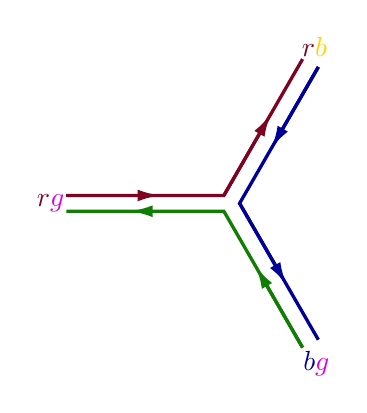
\begin{tikzpicture}[baseline=(current bounding box)]
            \draw [very thick, redgluoncolor] (-2, 0.1) -- (0, 0.1) -- ++ (60:2);
            \draw [very thick, greengluoncolor] (-2, -0.1) -- (0, -0.1) -- ++ (-60:2) coordinate (B);
            \path (0.2, 0) -- ++ (60:2) coordinate (A);
            \draw [very thick, bluegluoncolor] (A) -- (0.2, 0) -- ++ (-60:2);
            \draw [very thick, redgluoncolor, -{Latex[width=1.5mm]}] (-2, 0.1) -- (-0.8, 0.1);
            \draw [very thick, redgluoncolor, -{Latex[width=1.5mm]}] (0, 0.1) -- ++ (60:1.2);
            \draw [very thick, greengluoncolor, -{Latex[width=1.5mm]}] (0, -0.1) -- (-1.2, -0.1);
            \draw [very thick, greengluoncolor, -{Latex[width=1.5mm]}] (B) -- ++ (120:1.2);
            \draw [very thick, bluegluoncolor, -{Latex[width=1.5mm]}] (0.2, 0) -- ++ (-60:1.2);
            \draw [very thick, bluegluoncolor, -{Latex[width=1.5mm]}] (A) -- ++ (-120:1.2);
            \node at (-2.2, 0) {\(\Pred\APgreen\)};
            \node at (60:2.3) {\(\Pred\APblue\)};
            \node at (-60:2.35) {\(\Pblue\APgreen\)};
        \end{tikzpicture}
    \end{equation}
    
    
    \chapter{Running of Coupling Constants}
    \section{Renormalisation in QED}
    Consider the process \(\Pe \APe \to \Pmu \APmu\).
    The amplitude for this process can be computed as an infinite series.
    Each term of this series can then be understood as a particular process of particles and virtual particles interacting, which we depict as a Feynman diagram.
    So far we have always truncated this series at the tree level, meaning the diagrams have no loops.
    However, higher order terms in the series must be considered to increase accuracy.
    For example, a next to leading order term is given by the diagram
    \begin{equation}
        \tikzsetnextfilename{fd-nlo-electron-positron-to-muon-antimuon}
        \feynmandiagram[small, baseline=(current bounding box), horizontal=v1 to v3]{
            i1 [particle = \Pe] -- [fermion] v1 -- [fermion] v2 -- [fermion] i2 [particle = \APe],
            o1 [particle = \Pmu] -- [fermion] v3 -- [fermion] v4 -- [fermion] o2 [particle = \APmu],
            v1 -- [photon] v3,
            v2 -- [photon] v4
        };
    \end{equation}
    We can make an intuitive argument for why this diagram is less important than the tree level, leading order diagram.
    Each vertex gives a factor of \(e\), the magnitude of the charge of the electron.
    Hence, the leading order diagram has a factor of \(e^2 \propto \alpha\).
    The next to leading order term has twice as many vertices, so has a factor of \(e^4 \propto \alpha^2\), which makes this term \(137\) times smaller, all else being equal.
    
    Unfortunately this doesn't work.
    All else is \emph{not} equal.
    Part of the process for using the Feynman rules is to work out the momentum of each particle.
    Fixing some values \(p_i\) for the momenta of the initial and final particles we find that we can assign momenta as in the following diagram and momentum conservation is conserved at every vertex for any value we choose for \(k\):
    \begin{equation}
        \tikzsetnextfilename{fd-nlo-electron-positron-to-muon-antimuon-momenta}
        \feynmandiagram[baseline=(current bounding box), horizontal=v1 to v3]{
            i1 [particle = \Pe] -- [fermion, edge label = \(p_1\)] v1 -- [fermion, edge label = \(p_1 - k\)] v2 -- [fermion, edge label = \(p_2\)] i2 [particle = \APe],
            o1 [particle = \Pmu] -- [fermion, edge label' = \(p_3\)] v3 -- [fermion, edge label' = \(p_3 + k\)] v4 -- [fermion, edge label' = \(p_4\)] o2 [particle = \APmu],
            v1 -- [photon, momentum' = \(k\)] v3,
            v2 -- [photon, momentum = \(p_1 + p_2 - k\)] v4
        };
    \end{equation}
    Much like when we have a process with an undetermined spin we sum over it when we have a process with an undetermined momentum we integrate over it.
    In particular, the term in the series corresponding to this diagram has an integral of the form
    \begin{equation}
        \int \frac{^4k}{(2\pi)^4} f(k).
    \end{equation}
    The problem is, this doesn't converge.
    The solution is something called \defineindex{renormalisation}, where we redefine constants in such a way that all the infinities cancel.
    This is far beyond the scope of this course\footnote{See \course{Quantum Field Theory} for the basics of renormalisation and \course{Gauge Theories in Particle Physics} for the details pertaining to QED}.
    However, the key point is that we can take some infinite series of increasingly complex Feynman diagrams and recast the constants to be functions of the momentum of various particles in the diagrams in such a way that we can consider a single diagram.
    
    For example, consider the \(t\)-channel diagram
    \begin{equation}
        \tikzsetnextfilename{fd-renormalisation-in-QED-1}
        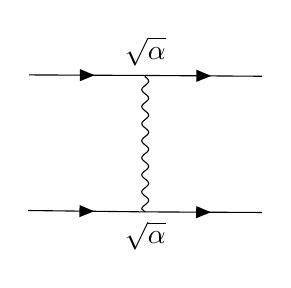
\begin{tikzpicture}[baseline=(current bounding box)]
            \begin{feynman}
                \diagram[vertical' = v1 to v2, small]{
                    i1 -- [fermion] v1 -- [fermion] o1,
                    i2 -- [fermion] v2 -- [fermion] o2,
                    v1 -- [photon] v2,
                    i1 -- [draw=none] i2,
                    o1 -- [draw=none] o2
                };
            \end{feynman}
            \node[above] at (v1) {\(\sqrt{\alpha}\)};
            \node[below] at (v2) {\(\sqrt{\alpha}\)};
        \end{tikzpicture}
    \end{equation}
    There are also higher order diagrams, such as
    \begin{equation}
        \tikzsetnextfilename{fd-renormalisation-in-QED-2}
        \begin{tikzpicture}[
                baseline=(current bounding box),
                photon/.style={decoration={snake, amplitude=1.25, segment length=6}, decorate},
                arrow/.style={-{Latex[width=1.5mm]}}
            ]
            \draw (0, 0) -- (4, 0);
            \draw (0, 4) -- (4, 4);
            \draw[photon] (2, 0) -- (2, 1);
            \draw[photon] (2, 3) -- (2, 4);
            \draw (2, 2) circle [x radius=0.7, y radius=1];
            \draw[arrow] (0, 0) -- ++ (1, 0);
            \draw[arrow] (2, 0) -- ++ (1, 0);
            \draw[arrow] (0, 4) -- ++ (1, 0);
            \draw[arrow] (2, 4) -- ++ (1, 0);
            \draw[arrow] (1.3, 2.07) -- ++ (0, 0.01);
            \draw[arrow] (2.7, 1.93) -- ++ (0, -0.01);
        \end{tikzpicture}
    \end{equation}
    
    We can replace this infinite series of diagrams with a single \(t\)-channel diagram, we simply replace \(\sqrt{\alpha}\) with a function of the momentum, \(\sqrt{\alpha(q^2)}\), where \(q\) is the momentum of the propagating photon.
    This is called \defineindex{running of the coupling constant}.
    It can be shown that
    \begin{equation}
        \alpha(q^2) = \frac{\alpha(\mu^2)}{1 - z_f\alpha(\mu^2) \ln(q^2/\mu^2)/(3\pi)}
    \end{equation}
    where \(\mu\) is some momentum for which we have a measured value of \(\alpha(\mu^2)\), and \(z_\varphi = \sum_{\Pf} Q_{\Pf}^2\) accounts for the all charged fermions, \(\Pf\), which can appear in the loop.
    
    We have very accurately measured \(\alpha\) at low, but nonzero, and crucially, known momenta, and we find a value of
    \begin{equation}
        \alpha(q^2 \approx 0) = \frac{1}{137.036}.
    \end{equation}
    We can also see that \(\alpha(q^2)\) is an increasing function of \(q^2\).
    This is born out in experiments.
    For example, at \(q = \qty{193}{\giga\electronvolt}\) we've measured \(\alpha(q^2) = 1/(127.4)\).
    
    \section{Renormalisation in QCD}
    Something similar happens in QCD.
    However, things are complicated by the fact that our loops can now include gluons, since they can interact with each other via the strong force.
    It can be shown that
    \begin{equation}
        \alpha_{\strongForce}(q^2) = \frac{\alpha_{\strongForce}(\mu^2)}{1 + B \alpha_{\strongForce}(\mu^2) \ln(q^2/\mu^2)}
    \end{equation}
    where
    \begin{equation}
        B = \frac{11\numberofcolors - 2N_{\Pq}}{12\pi},
    \end{equation}
    where \(\numberofcolors\) is the number of colours, \(3\), and \(N_{\Pq}\) is the number of accessible quarks at the energy of the process occurring.
    
    Unlike in QED in QCD \(\alpha_{\strongForce}\) is a decreasing function of \(q^2\).
    This means that at higher momenta we can treat QCD perturbatively, although for \(q^2 \approx m_{\PZ}^2\) we have \(\alpha_{\strongForce}(q^2) \approx 0.12\), and so we need to include an extra order of diagrams to get equivalent accuracy to low energy tree level QED predictions.
    
    In the limit of very high energies, or very small distances, \(\alpha_{\strongForce}\) essentially vanishes, and quarks and gluons behave like free particles.
    This is called \defineindex{asymptotic freedom}.
    
    \chapter{Jets and Partons}
    \section{Jets}
    The QCD potential goes as \(1/r\) at low energies.
    At higher energies the potential increases linearly with \(r\).
    This cannot be shown perturbatively since in this regime the value of \(\alpha_{\strongForce}(q^2)\) is too large.
    In fact the constant of proportionality is about \qty{1}{\giga\electronvolt\per\femto\metre}, so upon separating by \qty{1}{\femto\metre}, approximately the size of the atomic nucleus, the potential increases by \qty{1}{\giga\electronvolt}, this is a very large increase, especially compared to the masses of the quarks at \qty{2.3}{\mega\electronvolt} for an up quark.
    
    Consider the process of \(\Pe\APe \to \Pq\APq\) carried out at high energy.
    The quark-antiquark pair produced will initially have high velocity in the opposite direction in the centre of mass frame.
    This means they rapidly separate.
    The potential between them then increases until there is enough energy available for pair production, and a quark-antiquark pair will be produced.
    This takes some energy from the kinetic energy of the initial quarks in the centre of mass frame.
    The initial quarks will typically continue to separate, the potential increasing further, until there is enough energy to produced another quark-antiquark pair.
    This process repeats until the initial quark-antiquark pair are no longer becoming more separated.
    In the process many quark-antiquark pairs are formed, and these then form mesons and some baryons.
    These are mostly travelling in the same direction as the initial quark and antiquarks.
    We then get a number of hadrons all moving together.
    We call this a \defineindex{jet}.
    The process of producing the hadrons is called \defineindex{hadronisation}.
    
    Suppose that after producing the initial quark-antiquark pair one of the quarks produces a gluon.
    Then we'll also get a jet in the direction of this gluon, a so called \enquote{three jet event}.
    Observing three jet events like these was some of the firsts evidence for the existence of the gluon, since three particles with colour charge produced from a colour neutral \(\Pe\APe\) state must include a gluon.
    
    The branching ratio of three jet events to two jet events, that is the frequency of three jet events to the frequency of two jet events, gives us a good way to measure \(\strongCoupling\).
    The amplitude for one of the quarks to emit a gluon contains a factor of \(\strongCoupling\), and so the cross section for the three jet event will be proportional to \(\strongCoupling^2\).
    An exact computation of the cross sections can then tell us the expected branching ratio as a function of \(\strongCoupling\), which we can then compare to measurements.
    
    Despite involving quarks and being used to probe QCD the process \(\Pe\APe \to \Pq\APq\) is a QED process.
    In particular, it is an example of \(\Pe\APe \to \Pf\APf\), and we've already seen this type of process.
    We know that the differential cross section for this process is
    \begin{equation}
        \diff{\sigma}{\Omega} = \frac{\alpha^2}{4s}(1 + \cos^2\vartheta),
    \end{equation}
    and this measurements compared to this result provided good evidence that quarks are indeed spin \(1/2\) fermions.
    
    The added benefit of using a QED process to probe the strong force is that QED is very well understood.
    It's also cleaner experimentally.
    Electrons are, to the best of our knowledge, fundamental point particles, and don't have internal structure.
    Something like proton-proton scattering, such as in the LHC, is much messier, since the result depends on the structure of the proton, which isn't a fundamental particle, and we also don't get complete interactions, we'll typically have some remanents of the proton left over after the collision.
    This is part of the reason why we typically start with electron-positron colliders each time we build a bigger collider at higher energies (like LEP), and then build a proton-proton collider afterwards (like the LHC).
    
    It is not, in general, possible to tell which jet forms from the quark and which jet forms from the proton.
    There have been recent developments using machine learning to make this identification, but it's far from perfect.
    This machine learning technique does have a slightly higher ability to identify a jet coming from a gluon.
    
    Recall that the amplitude for the process \(\Pe\APe \to \Pf\APf\) is
    \begin{equation}
        -i\amplitude(\Pe\APe \to \Pf\APf) = \frac{Q_{\Pf}e^2}{s} j_{\symrm{e}} \cdot j_{\Pf}.
    \end{equation}
    We can then measure the ratio
    \begin{equation}
        R = \frac{\sigma(\Pe\APe \to \text{hadrons})}{\sigma(\Pe\APe \to \Pmu\APmu)}.
    \end{equation}
    Most parts, all the dynamics, cancel in this ratio, and we're left with just
    \begin{equation}
        R = \numberofcolors \sum_{\text{flavours}} Q_{\Pq}^2
    \end{equation}
    where the sum is over all flavours of quarks with \(2m_{\Pq} < \sqrt{s}\).
    Both experimental and theoretical values for \(R\) are plotted in \cref{fig:R ratio}.
    
    By measuring \(R\) at different values of \(\sqrt{s}\), we see \(R\) is mostly flat, with sudden jumps up at energies corresponding to a new flavour of quark becoming accessible.
    As well as this we also see resonances, large peaks in the cross section, for bound states of quarks\footnote{these are from poles, as in \(1/0\), in the amplitude when particles go on-shell. See \course{Quantum Field Theory} for details.}.
    If these consist of a quark and its antiquark, such as the\footnote{the \PJpsi{} was discovered independently by two experiments who gave it different names, the name is a combination of the two names they chose.} \PJpsi{} which is \(\Pc\APc\), then they become accessible just before a free quark-antiquark pair becomes accessible, so these spikes are another way to narrow down the masses of the quarks.
    As well as being evidence for the masses of quarks the value of \(R\) is also evidence that \(\numberofcolors = 3\).
    
    \begin{figure}
        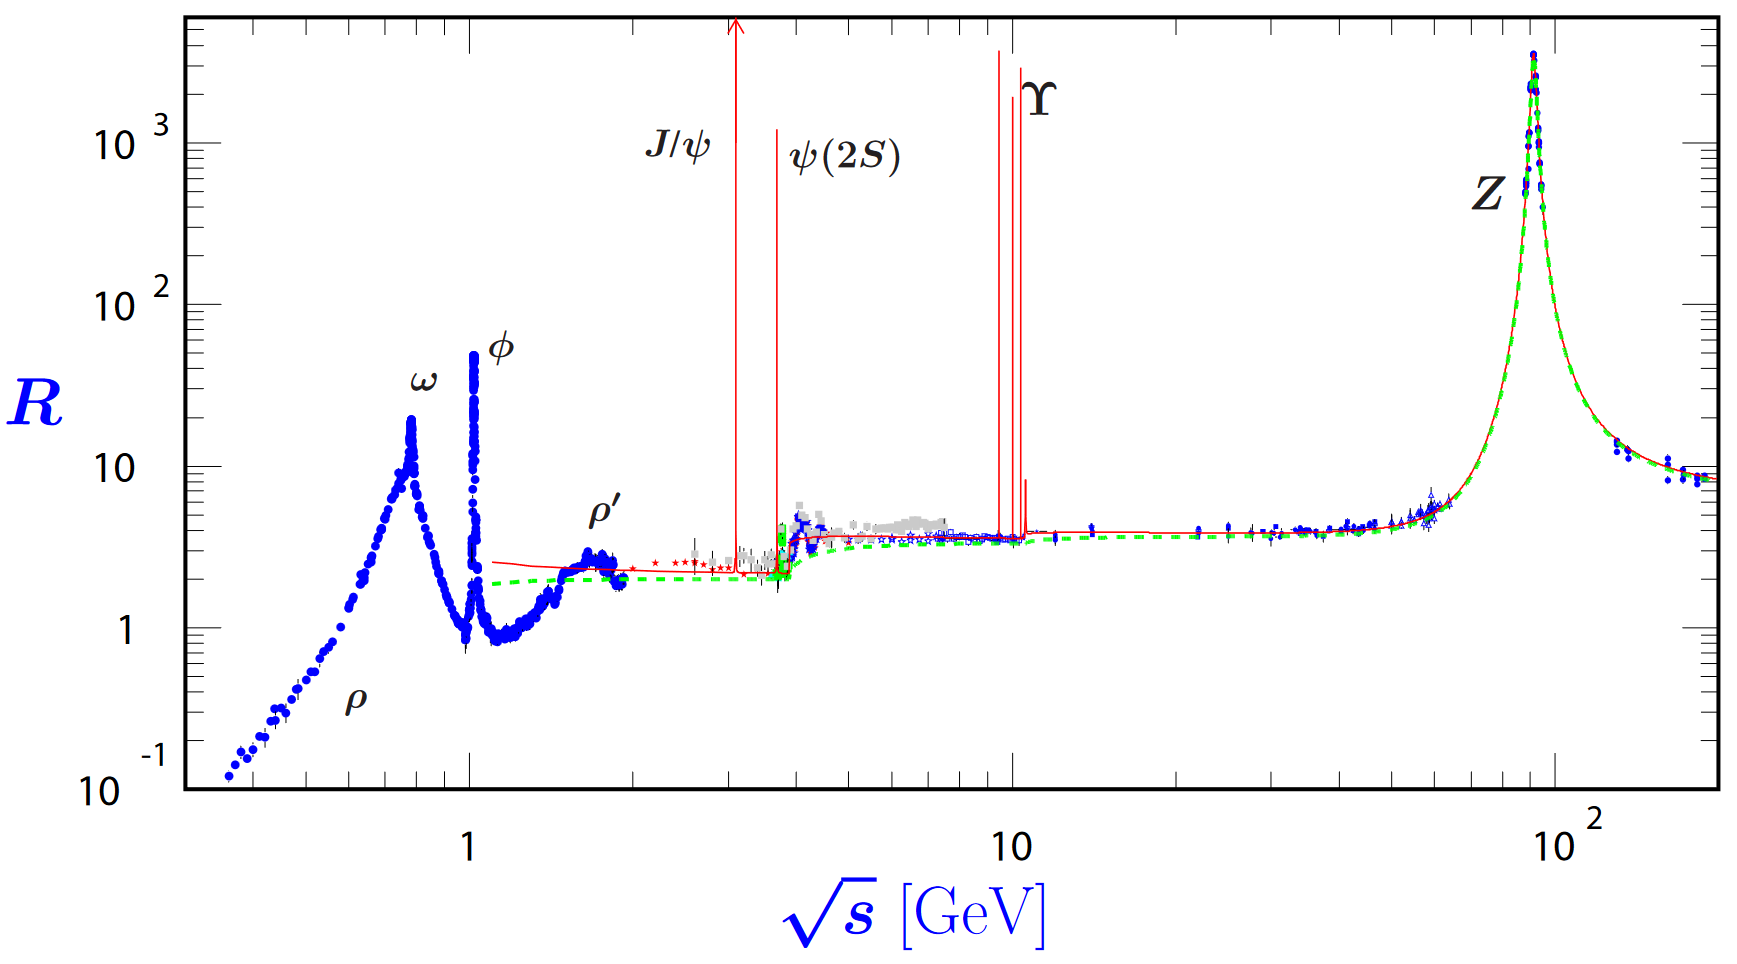
\includegraphics[width=0.8\textwidth]{images/hadron-muon-branching-ratio}
        \caption[Hadron to muon branching ratio.]{The ratio \(R = \sigma(\Pe\APe \to \text{hadrons})/\sigma(\Pe\APe \to \Pmu\APmu)\) measured and predicted as a function of \(\sqrt{s}\), the centre of mass frame energy. Note that, ignoring the peaks, we see that \(R\) is flat with sudden steps upwards at, approximately, \(\sqrt{s} = \qtylist{4,10}{\giga\electronvolt}\), corresponding to the charm and bottom quarks becoming accessible. We also see resonances for the bound quark states \(\text{\normalfont φ}\) (\(\Ps\APs\)), \PJpsi{} (\(\Pc\APc\)), \(\text{\normalfont ψ}(2S)\) (\(\Pc\APc\)), and \(\text{\normalfont Υ}\) (\(\Pb\APb\)), as well as the \PZ{} boson. At lower energies we also see the states \(\text{\normalfont ρ}\), \(\text{\normalfont ω}\), and \(\text{\normalfont ρ'}\). These are more complex superpositions of bound quark states, and are related by \(\specialUnitary(3)\) symmetries. Figure taken from lecture notes, unable to find original source.}
        \label{fig:R ratio}
    \end{figure}
    
    \section{Proton-Proton Collisions}
    Protons have three quarks, \(\Pu\Pu\Pd\).
    These quarks, called the \define{valence quarks}\index{valence quark} are always present at any energy scale.
    However, at high energies interactions between these quarks produce a sea of virtual quarks in quark-antiquark pairs, as well as gluons.
    We call particles within a proton \define{partons}\index{parton}.
    At high energies when we have a collision between protons it occurs on the level of these partons interacting.
    This makes proton-proton collisions significantly more complicated than electron-positron collisions.
    
    One quantity that is useful to know about a parton is the so called \define{Bjorken \(\symbf{x}\)}\index{Bjorken x@Bjorken \(x\)}.
    It is defined as the ratio of the momentum of that parton to the momentum of the proton it is in,
    \begin{equation}
        x \coloneqq \frac{p(\text{parton})}{p(\text{proton})}.
    \end{equation}
    This is a Lorentz invariant, and is useful when trying to work out exactly which physics is relevant at a given scale.
    Note that \(x \in [0, 1]\).
    
    Define \(q^{\Pp}(x)\) to be such that \(q^{\Pp}(x)\dd{x}\) is the number of quarks of flavour \(q\), or more generally any particle, \(q\), within a proton with momentum between \(x\) and \(x + \dl{x}\).
    Note that we consider averages, so this needn't be an integer.
    We call \(q^{\Pq}\) the \defineindex{parton distribution function}, or PDF\glossary[acronym]{PDF}{parton distribution function}.
    
    The simplest case is when we treat the proton, a spin \(1/2\) particle, as a Dirac fermion satisfying the Dirac equation.
    We then completely ignore the internal structure, and so \(q^{\Pp}(x) = Q^2\delta(x - 1)\) where \(Q\) is the momentum of the proton, that is, all of the momentum is concentrated in a singular particle.
    The next simplest case is three noninteracting quarks.
    In this case \(q^{\Pp}(x) = Q^2\delta(x - 1/3)\), that is each quark has \(1/3\) of the momentum.
    A more realistic model is given by consider three quarks and first order interactions.
    Then the momentum is more spread out.
    Considering higher order interactions increases the proportion of low momentum particles, since the particles produced in higher order interactions tend to have lower momentum, since the amplitude contains factors of \(1/q^2\).
    See \cref{fig:parton distribution function} for a plot of parton distribution functions for the valence quarks, gluons and other quarks.
    
    At high momenta, such as in the LHC, the gluons carry a significant portion of the momentum of the proton, and there's a lot of them.
    For this reason some people say the LHC is really a gluon-gluon collider.
    
    \begin{figure}
        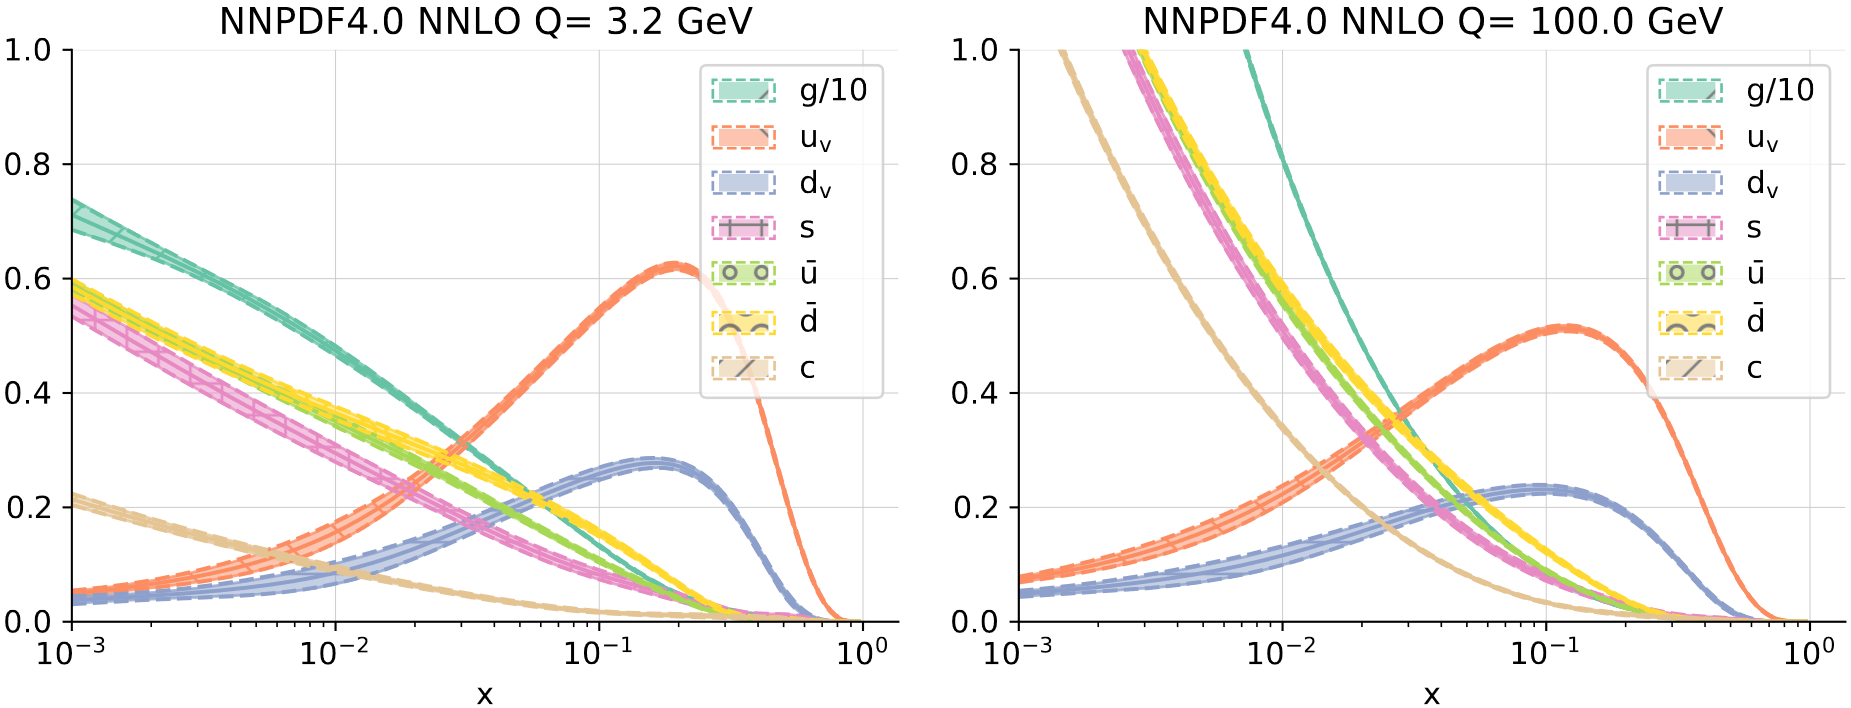
\includegraphics[width=0.9\textwidth]{images/parton-distribution-function}
        \caption[Parton distribution function]{Parton distribution functions at proton momenta \(Q = \qty{3.2}{\giga\electronvolt}\), and \(Q = \qty{100}{\giga\electronvolt}\). Notice that at \(Q = \qty{3.2}{\giga\electronvolt}\) the distributions for up and down quarks peak at about \(0.2\), so the quarks carry just under a third of the energy each, at \(Q = \qty{100}{\giga\electronvolt}\) they instead peak at about \(0.02\), so the valence quarks have a much small fraction of the total momentum. Notice that the peak for the up quarks is about twice as high as for the down quarks, since there are twice as many up quarks. Note that in both plots we divide the parton function for the gluons by 10, since it becomes very large at small \(x\), essentially we have lots of low momentum gluons. At \(Q = \qty{100}{\giga\electronvolt}\) the gluons carry a non-negligible proportion of the protons momentum. Figure taken from \cite{ball}.}
        \label{fig:parton distribution function}
    \end{figure}
    
    \part{Weak Interactions}
    \chapter{Weak Interactions}
    \section{Parity}
    We've seen that parity is the symmetry given by inverting space, sending \((t, \vv{x})\) to \((t, -\vv{x})\).
    For spinors we saw that this is exactly the effect of the \(\gamma^0\) matrix.
    We then defined the parity of particles, that is, negative leptons, neutrinos and quarks, to be \(1\), and the parity of antiparticles, that is, positive leptons, antineutrinos and antiquarks, to be \(-1\).
    We saw that parity transformations take right handed helicity states to right handed helicity states, and vice versa, as well as taking left handed chiral states to right handed chiral states, and vice versa.
    
    Experimentally we see that QED and QCD are invariant under parity inversions.
    This means left and right handed states are treated equally by QED and QCD.
    In terms of the maths this arises from the amplitude being proportional to \(j_1 \cdot j_2\), where \(j_i\) are of the form
    \begin{equation}
        j_i^\mu = \overbar{\psi} \gamma^\mu \varphi,
    \end{equation}
    for some Dirac spinors \(\psi\) and \(\varphi\).
    Regardless, under parity we have \(\psi \mapsto \gamma^0 \psi\) for any Dirac spinor, \(\psi\).
    Thus we have \(\diracadjoint{\psi} = \psi^\hermit \gamma^0 \mapsto (\gamma^0\psi)^\hermit\gamma^0 = \psi^\hermit (\gamma^0)^\hermit \gamma^0 = \psi^\hermit \gamma^0 \gamma^0 = \diracadjoint{\psi}\gamma^0\), using \((\gamma^0)^\hermit = \gamma^0\).
    We then have
    \begin{equation}
        j_i^\mu = \diracadjoint{\psi} \gamma^\mu \varphi \mapsto \diracadjoint{\psi} \gamma^0 \gamma^\mu \gamma^0 \varphi.
    \end{equation}
    Now consider the temporal component, we have \((\gamma^0)^3 = \gamma^0\) and so \(j_i^0 \mapsto j_i^0\).
    For the spatial components we have \(\gamma^0 \gamma^j \gamma^0 = -\gamma^j (\gamma^0)^2 = -\gamma^j\), using \((\gamma^0)^2 = 1\) and the anticommutativity of the gamma matrices with different Lorentz indices, which comes from the defining relation \(\anticommutator{\gamma^\mu}{\gamma^\nu} = 2\minkowskiMetric^{\mu\nu}\).
    Hence, we have \(j_i^j \mapsto -j_i^j\).
    So under parity the spatial components of the fermion current are inverted.
    This means that the product \(j_1 \cdot j_2\) transforms as
    \begin{equation}
        j_1 \cdot j_2 = j_1^0 j_2^0 - \vv{j}_1 \cdot \vv{j}_2 \mapsto j_1^0 j_2^0 - (-\vv{j}_1) \cdot (-\vv{j}_2) = j_1 \cdot j_2
    \end{equation}
    under parity.
    That is, noting changes.
    
    Note that everything here holds for both QED and QCD, since the Feynman rules differ only by terms unaffected by parity, such as charges, coupling constants, and colour factors.
    The result is that in both QED and QCD parity is conserved, it is a \enquote{good} symmetry.
    
    \section{Parity Violation}
    Parity is not conserved in all interactions, in fact, in weak interactions not only is parity not conserved, but parity conservation is, in a sense, maximally violated.
    This was first observed in the beta decay of cobalt in a magnetic field.
    The decay equation is
    \begin{equation}
        \ce{^60Co -> ^60Ni^*+ {\Pe} + \APnue}.
    \end{equation}
    On the level of quarks this decay is
    \begin{equation}
        \Pd \to \Pu + \Pe + \APnue.
    \end{equation}
    In this experiment researchers measured the angular distribution of the emitted electrons.
    They found that some angles were much more likely than others.
    The cobalt nucleus has spin \(J = 5\), and the nickel spin \(J = 4\).
    Performing the experiment in a strong magnetic field meant that the \(z\)-components of these spins, measured in the direction of the field, were maximised.
    Conservation of angular momentum then requires that the electron and antineutrino have spin \(J = 1/2\).
    
    In the experiment more electrons were emitted in the \(-z\) direction, but there spin was oriented in the \(+z\) direction, and hence these were left-handed particles.
    The conclusion is that left-handed particles are preferentially produced in this interaction.
    
    \section{Charged Current Weak Interactions}
    This requires a fundamentally different form to the mathematics of the weak equation, not just extra factors like we found when going from QED to QCD.
    In QED and QCD we have the four-vector fermion current, \(j^\mu\), defined as an adjoint spinor times \(\gamma^\mu\) times a spinor.
    This is not the only Lorentz invariant combination of spinors, in fact there are five distinct ways to combine two spinors to form a Lorentz covariant object from which we can form a Lorentz invariant by contracting it with another similar object, these are\footnote{see \course{Quantum Field Theory} or \course{Symmetries of Particles and Fields} for details. All other combinations can be decomposed into a sum and/or product of these.}
    \begin{center}
        \begin{tabular}{lccc}
            \toprule
            Type & Form & Components & Spin\\ \midrule
            Scalar & \(\diracadjoint{\psi} \varphi\) & 1 & 0\\
            Pseudoscalar & \(\diracadjoint{\psi} \gamma^5 \varphi\) & 1 & 0\\
            Vector & \(\diracadjoint{\psi} \gamma^\mu \varphi\) & 4 & 1\\
            Axial Vector & \(\diracadjoint{\psi} \gamma^\mu \gamma^5 \varphi\) & 4 & 1\\
            Tensor & \(\diracadjoint{\psi} (\gamma^\mu \gamma^\nu - \gamma^\nu \gamma^\mu) \varphi\) & 6 & 2\\\bottomrule
        \end{tabular}
    \end{center}
    
    It is the vector current which we see in QED and QCD.
    For now we consider \PWpm{} boson interactions.
    The current for \PWpm{} bosons is of the form
    \begin{equation}
        \diracadjoint{\psi} \gamma^\mu (\ident - \gamma^5)\varphi = \diracadjoint{\psi} \gamma^\mu \varphi - \diracadjoint{\psi}\gamma^\mu \gamma^5 \varphi = \text{vector} - \text{axial vector}.
    \end{equation}
    Under parity the spatial part of the vector is inverted but the spatial part of the axial vector is unchanged.
    This means that parity is not a symmetry of this current, which is what we expect for the weak force.
    
    Recall that we can define the chiral projection operators,
    \begin{equation}
        P_{\Right} = \frac{1}{2}(1 + \gamma^5), \qqand P_{\Left} = \frac{1}{2}(1 - \gamma^5).
    \end{equation}
    Any spinor can be expressed as a sum of its left and right components,
    \begin{equation}
        \psi = P_{\Right}\psi + P_{\Left}\psi = \psi_{\Right} + \psi_{\Left},
    \end{equation}
    i.e., \(\{P_{\Right}, P_{\Left}\}\) is a complete set of operators.
    For a vector current this means that we had
    \begin{equation}
        \diracadjoint{\psi}\gamma^\mu \varphi = \diracadjoint{\psi}_{\Right}\gamma^\mu \varphi_{\Right} + \diracadjoint{\psi}_{\Left}\gamma^\mu \varphi_{\Left},
    \end{equation}
    since we could show that \(\diracadjoint{\psi}_{\Left}\gamma^\mu\varphi_{\Right}\) and \(\diracadjoint{\psi}_{\Right}\gamma^\mu\varphi_{\Left}\) are identically zero.
    In the ultrarelativistic limit, where chiral states and helicity states are equivalent, this lead to there only being two nonzero contributions to the fermion current.
    
    Now considering the charged current, which is just another way of saying the \PWpm{} boson current, we have
    \begin{equation}
        \diracadjoint{\psi} \gamma^\mu (1 - \gamma^5) \varphi = 2\diracadjoint{\psi}\gamma^\mu \varphi_{\Left} = 2(\diracadjoint{\psi}_{\Right} + \diracadjoint{\psi}_{\Left})\gamma^\mu\varphi_{\Left} = 2\diracadjoint{\psi}_{\Left} \gamma^\mu \varphi_{\Right}.
    \end{equation}
    So, we see that only the left-handed states contribute to the current.
    
    Using this we can list all possible charged weak vertices involving, say, an electron and neutrino:
    \begin{itemize}
        \item left-handed electron, left-handed neutrino, and a \PW{} boson,
        \item right-handed positron, left-handed neutrino, and a \PW{} boson,
        \item left-handed electron, right-handed antineutrino, and a \PW{} boson,
        \item right-handed positron, right-handed antineutrino, and a \PW{} boson.
    \end{itemize}
    
    \section{Pion Decay}
    Consider the decay of a negative pion, \Ppim, which is formed from two quarks, \(\Pd\APu\), and has mass \(m_{\Ppim} = \qty{139}{\mega\electronvolt}\).
    Given the mass of the pion there are two ways that this can occur,
    \begin{equation}
        \Ppim \to \Pe \APnue, \qqor \Ppim \to \Pmu \APnumu.
    \end{equation}
    Since both processes occur via the same mechanism one may initially expect that the amplitudes for both are about the same.
    Then one would expect that since the electron is much lighter, \(m_{\symrm{e}} = \qty{511}{\kilo\electronvolt}\), than the muon, \(m_{\text{\normalfont μ}} = \qty{105}{\mega\electronvolt}\), the increased volume of phase space for the electron decay, due to the increased amount of momentum after the decay, and hence increased number of ways of distributing the momentum, should mean that the decay width\footnote{a measure of probability of a given decay channel, with units of energy} for decay to an electron should be much larger.
    
    However, experimentally we find
    \begin{equation}
        \frac{\Gamma(\Ppim \to \Pe \APnue)}{\Gamma(\Ppim \to \Pmu \APnumu)} = \num{1.23e-4}.
    \end{equation}
    So in fact decay into a muon is about a thousand times more likely than decay into a electron.
    The reason for this is that the electron channel is helicity suppressed.
    
    Work in the rest frame of the pion and consider decay into an electron and electron antineutrino.
    Conservation of angular momentum, since the pion has spin 0, requires that the spin of the electron and neutrino are opposite.
    Since this is a weak interaction the electron must be in a left-handed chiral state.
    Similarly the antineutrino must be in a right handed chiral state.
    Treat the antineutrino as massless.
    Then it is also in a right handed helicity state.
    This means that its spin is aligned with its momentum.
    The momentum of the electron and the spin of the electron are both opposite the spin spin and momentum of the antineutrino respectively, hence they are also aligned.
    So, the electron is in a right-handed helicity state.
    But we've already seen that the electron is in a left-handed chiral state.
    
    In order to compute the amplitude for decay into an electron we need to compute the overlap of the left-handed chiral state and the right-handed helicity state.
    This can be done by acting on the right-handed helicity state with the projection operators:
    \begin{equation}
        u_{\uparrow} = P_{\Right}u_{\uparrow} + P_{\Left}u_{\uparrow} = \frac{1}{2}\left( 1 + \frac{\abs{\vv{p}}}{E + m} \right)u_{\Right} + \frac{1}{2}\left( 1 - \frac{\abs{\vv{p}}}{E + m} \right)u_{\Left}.
    \end{equation}
    The matrix element will be proportional to the left-handed chiral component of the electron, that is
    \begin{equation}
        \amplitude \propto \frac{1}{2}\left( 1 - \frac{\abs{\vv{p}}}{E + m} \right).
    \end{equation}
    In the rest frame of the pion the momentum of the pion is \(p_{\Ppi}^\mu = (m_{\Ppim}, \vv{0})\), the momentum of the electron is \(p^\mu_{\symrm{e}} = (E_{\symrm{e}}, \vv{p})\) and the momentum of the antineutrino is \(p^\mu_{\text{\normalfont ν}} = (E_{\text{\normalfont ν}}, -\vv{p})\).
    Then we have
    \begin{equation}
        p_{\Ppi} = p_{\symrm{e}} + p_{\text{\normalfont ν}} \implies p_{\text{\normalfont ν}} = p_{\Ppi} - p_{\symrm{e}} \implies (p_{\Ppi} - p_{\symrm{e}})^2 = p_{\text{\normalfont ν}}^2 = m_{\text{\normalfont ν}}^2 \approx 0,
    \end{equation}
    and expanding then gives
    \begin{equation}
        0 \approx p_{\Ppi}^2 + p_{\symrm{e}}^2 - 2 p_{\Ppi} \cdot p_{\symrm{e}} = m_{\Ppim}^2 + m_{\symrm{e}}^2 - 2m_{\Ppim}E_{\symrm{e}}.
    \end{equation}
    Rearranging this we have
    \begin{equation}
        E_{\symrm{e}} = \frac{m_{\Ppim}^2 + m_{\symrm{e}}^2}{2m_{\Ppim}}.
    \end{equation}
    We also have
    \begin{equation}
        p_{\symrm{e}} = p_{\Ppi} - p_{\text{\normalfont ν}} \implies p_{\symrm{e}}^2 = m_{\symrm{e}}^2 = p_{\Ppi}^2 + p_{\text{\normalfont ν}}^2 - 2p_{\Ppi} \cdot p_{\text{\normalfont ν}} \approx m_{\Ppim}^2 - 2 m_{\Ppim} E_\nu
    \end{equation}
    giving
    \begin{equation}
        E_{\text{\normalfont ν}} = \frac{m_{\Ppim}^2 - m_{\symrm{e}}^2}{2m_{\Ppim}}.
    \end{equation}
    If \(m_{\text{\normalfont ν}} = 0\) then we have \(E_{\text{\normalfont ν}} = \abs{\vv{p}}\), so we can also say that
    \begin{equation}
        \abs{\vv{p}} = \frac{m_{\Ppim}^2 - m_{\symrm{e}}^2}{2m_{\Ppim}}.
    \end{equation}
    Combing these results we have
    \begin{align}
        1 - \frac{\abs{\vv{p}}}{E_{\symrm{e}} + m_{\symrm{e}}} &= \frac{E_{\symrm{e}} + m_{\symrm{e}} - \abs{\vv{p}}}{E_{\symrm{e}} + m_{\symrm{e}}}\\
        &= \frac{\frac{m_{\Ppim}^2 + m_{\symrm{e}}^2}{2m_{\Ppim}} + m_{\symrm{e}} - \frac{m_{\Ppim}^2 - m_{\symrm{e}}^2}{2m_{\Ppim}}}{{\frac{m_{\Ppim}^2 + m_{\symrm{e}}^2}{2m_{\Ppim}}} + m_{\symrm{e}}}\\
        &= \frac{m_{\Ppim}^2 + m_{\symrm{e}}^2 + 2m_{\Ppim}m_{\symrm{e}} - m_{\Ppim}^2 + m_{\symrm{e}}^2}{m_{\Ppim}^2 + m_{\symrm{e}}^2 + 2m_{\Ppim}m_{\symrm{e}}}\\
        &= \frac{2m_{\symrm{e}}^2 + 2m_{\Ppim}m_{\symrm{e}}}{m_{\Ppim}^2 + m_{\symrm{e}}^2 + 2m_{\Ppim}m_{\symrm{e}}}\\
        &= \frac{2m_{\symrm{e}}(m_{\symrm{e}} + m_{\Ppim})}{(m_{\Ppim} + m_{\symrm{e}})^2}\\
        &= \frac{2m_{\symrm{e}}}{m_{\Ppim} + m_{\symrm{e}}}.
    \end{align}

    So,
    \begin{equation}
        \amplitude(\Ppim \to \Pe \APe) \propto \frac{m_{\symrm{e}}}{m_{\Ppim} + m_{\symrm{e}}} \approx 0.0037.
    \end{equation}
    Similarly,
    \begin{equation}
        \amplitude(\Ppim \to \Pmu \APmu) \propto \frac{m_{\text{\normalfont  μ}}}{m_{\Ppim} + m_{\text{\normalfont  μ}}} \approx 0.43.
    \end{equation}
    So, all else being equal we would expect decay to a muon to be much more likely.
    
    \chapter{More Weak Interactions}
    \section{\PW{} Boson Propagator}
    The \PW{} boson differs from other bosons we've seen, the photon and gluons, in that the \PW{} boson is massive.
    It has a mass of\footnote{Recent measurements place the mass slightly higher at \(m_{\PW} = \qty{80.433(9)}{\giga\electronvolt}\), the reason for the difference is not known, it could be experimental error or perhaps a glance at some physics beyond the standard model.} \(m_{\PW} = \qty{80.379(12)}{\giga\electronvolt}\).
    This is not just nonzero, but actually quite large.
    Being a massive particle the \PW{} boson does \emph{not} travel at the speed of light.
    This means that it has an extra polarisation state, longitudinal, since the field can oscillate in the direction of travel without violating causality.
    The result is that we have to modify the propagator for \PW{} bosons with an extra term, for a \PW{} boson with momentum \(q\) the propagator is
    \begin{equation}
        \frac{-i}{q^2 - m_{\PW}^2}\left( \minkowskiMetric_{\mu\nu} - \frac{q_\mu q_\nu}{m_{\PW}^2} \right).
    \end{equation}
    This is derived in \cref{sec:massive gauge bosons}.
    Note that instead of \(1/q^2\) as for the photon and gluon we have \(1/(q^2 - m_{\PW}^2)\).
    
    If \(q^2 \ll m_{\PW}^2\) then we can often, practically always in this course, get away with the approximation
    \begin{equation}
        \frac{-i\minkowskiMetric_{\mu\nu}}{q^2 - m_{\PW}^2}.
    \end{equation}
    In the limit of even lower energy interactions, \(q^2 \lll m_{\PW}^2\), we can further approximate the propagator as
    \begin{equation}
        \frac{i\minkowskiMetric_{\mu\nu}}{m_{\PW}^2}.
    \end{equation}
    Notice that this is independent of the momentum transferred by the \PW{} boson.
    
    We can now give the Feynman rules for weak interactions involving the \PW{} boson.
    For external fermions they are the same as for QED, these rules are listed in \cref{sec:feynman rules QED}.
    For an internal \PW{} boson propagator of momentum \(q\) we have
    \begin{equation}
        \frac{-i}{q^2 - m_{\PW}^2} \left( \minkowskiMetric_{\mu\nu} - \frac{q_\mu q_\nu}{m_{\PW}^2} \right) \approx \frac{-i\minkowskiMetric_{\mu\nu}}{q^2 - m_{\PW}^2} \approx \frac{i\minkowskiMetric_{\mu\nu}}{m_{\PW}^2}.
    \end{equation}
    For a vertex joining two fermions and a \PW{} boson we get a vertex term
    \begin{equation}
        \frac{-ig_{\PW}}{\sqrt{2}} \frac{1}{2}\gamma^\mu (1 - \gamma^5)
    \end{equation}
    where \(g_{\PW}\) is a coupling constant.
    This is almost the same as in QED and QCD but we replace the vector current with a vector current minus an axial vector current.
    We also include an extra factor of \(1/\sqrt{2}\), for historical reasons\footnote{Initially \(g_{\PW}\) was defined without regard for parity violations.}.
    \begin{wrn}
        This isn't quite right for weak interactions involving quarks, see \cref{sec:weak interactions with quarks}.
    \end{wrn}
    
    \section{Fermi Theory}
    Before the existence of the \PW{} boson was known Fermi showed that, at least at low energies, it was possible to describe the effects of charged current weak interactions with an effective field theory involving a four point vertex.
    He imagined a process that we now know as occurring via a \PW{} boson, such as
    \begin{equation}
        \tikzsetnextfilename{fd-weak-interaction-not-via-fermi-theory}
        \feynmandiagram[vertical=v1 to v2, baseline=(current bounding box)]{
            i1 [particle=\Pnue] -- [fermion, edge label'=\(p_1\)] v1 -- [fermion, edge label'=\(p_3\)] o1 [particle=\Pe],
            i2 [particle=\Pd] -- [fermion, edge label=\(p_2\)] v2 -- [fermion, edge label=\(p_4\)] o2 [particle=\Pu],
            v1 -- [boson, edge label=\PW] v2
        };
    \end{equation}
    as occurring without a propagator:
    \begin{equation}
        \tikzsetnextfilename{fd-weak-interaction-via-fermi-theory}
        \feynmandiagram[baseline=(current bounding box)][rotate=135]{
            i2 [particle=\Pd] -- [fermion, edge label=\(p_2\)] v [dot] -- [fermion, edge label=\(p_4\)] o2 [particle=\Pu],
            i1 [particle=\Pnue] -- [fermion, edge label'=\(p_1\)] v -- [fermion, edge label'=\(p_3\)] o1 [particle=\Pe]
        };
    \end{equation}
    
    Heuristically, at low energies the \PW{} boson can't propagate very far before decaying, since it's massive, and Fermi theory is just the limit where it doesn't propagate at all.
    
    Fermi theory then predicts the amplitude for this process to be
    \begin{equation}
        \amplitude = -\fermiConstant[\overbar{u}(p_3) \gamma^\mu u(p_1)] \minkowskiMetric_{\mu\nu} [\overbar{u}(p_4) \gamma^\nu u(p_2)],
    \end{equation}
    with \(\fermiConstant\) a coupling constant, called the \defineindex{Fermi constant}, just like \(e\) in QED or \(\strongCoupling\) in QCD.
    After allowing for parity violation, which we'll see later, we instead get
    \begin{equation}
        \amplitude = -\frac{\fermiConstant}{\sqrt{2}} [\diracadjoint{u}(p_3) \gamma^\mu (1 - \gamma^5) u(p_1)] \minkowskiMetric_{\mu\nu} [\diracadjoint{u}(p_4) \gamma^\nu (1 - \gamma^5) u(p_2)].
    \end{equation}
    The full result using our modern understanding of the weak force and the \PW{} boson is
    \begin{equation}
        \amplitude = -\frac{g_{\PW}^2}{2} \left[ \diracadjoint{u}(p_3) \gamma^\mu \frac{1}{2}(1 - \gamma^5)u(p_1) \right] \frac{\minkowskiMetric_{\mu\nu} - q_\mu q_\nu/m_{\PW}^2}{q^2 - m_{\PW}^2} \left[ \diracadjoint{u}(p_4) \gamma^\nu \frac{1}{2}(1 - \gamma^5) u(p_2) \right].
    \end{equation}
    In the limit of low \(q^2\) this reduces to
    \begin{equation}
        \amplitude = -\frac{g_{\PW}^2}{8m_{\PW}^2} [\diracadjoint{u}(p_3) \gamma^\mu (1 - \gamma^5) u(p_1)] \minkowskiMetric_{\mu\nu} [\diracadjoint{u}(p_4) \gamma^\nu(1 - \gamma^5) u(p_2)].
    \end{equation}
    Comparing this with the result of Fermi theory we find that
    \begin{equation}
        \frac{\fermiConstant}{\sqrt{2}} = \frac{g_{\PW}^2}{8m_{\PW}^2}.
    \end{equation}
    
    \section{Measuring the Fermi Constant}
    We can measure \(\fermiConstant\) by considering muon decay.
    There is only really\footnote{the next most likely decay is \(\Pmu \to \Pe\Pnumu\APnue\Pe\APe\), this occurs with probability \(\num{3e-5}\), other decays are a thousand times less likely again.} one decay channel for muons, \(\Pmu \to \Pe\Pnumu\APnue\).
    This corresponds to
    \begin{equation}
        \tikzsetnextfilename{fd-muon-decay}
        \feynmandiagram[layered layout, horizontal=i to v1, baseline=(i)]{
            i [particle=\Pmu] -- [fermion, edge label=\(p_1\)] v1,
            v1 -- [fermion, edge label=\(p_2\)] o1 [particle=\Pnumu],
            v1 -- [boson, edge label'=\PW] v2,
            v2 -- [fermion, edge label=\(p_3\)] o2 [particle=\Pe],
            v2 -- [anti fermion, edge label'=\(p_4\)] o3 [particle=\APnue]
        };
    \end{equation}
    We expect that
    \begin{equation}
        \amplitude \propto \frac{g_{\PW}^2}{8m_{\PW}^2} = \frac{\fermiConstant}{\sqrt{2}} \implies \amplitude^2 \propto \frac{g_{\PW}^5}{64 m_{\PW}^4} = \frac{\fermiConstant^2}{2}.
    \end{equation}
    The decay width, \(\Gamma(\Pmu \to \Pe \Pnumu \APnue)\), is given by \(\amplitude^2\) times a phase space term.
    The units of \(\Gamma\) are energy, and the units of \(\amplitude^2\) are energy to the minus 4, so the phase space term must have units of energy to the fifth power.
    The only real energy scale that we have is the mass of the muon, the masses of the electron and neutrinos are negligible compared to this.
    We then posit that the phase space term is proportional to \(m_{\upmu}^5\).
    A full calculation bears this out and gives the result
    \begin{equation}
        \Gamma(\Pmu \to \Pe \Pnumu \APnue) = \frac{\fermiConstant m_{\upmu}^5}{192 \pi^3}.
    \end{equation}
    
    The total decay width, \(\Gamma_{\symrm{tot}}\), is pretty much exactly \(\Gamma(\Pmu \to \Pe \Pnumu \APnue)\).
    The lifetime of the muon is
    \begin{equation}
        \tau_{\upmu} = \frac{1}{\Gamma_{\symrm{tot}}} = \frac{1}{\Gamma(\Pmu \to \Pe \Pnumu \APnue)}.
    \end{equation}
    
    Putting in measured values for \(m_{\upmu}\), \(\tau_{\upmu}\), and \(m_{\PW}\) we find that
    \begin{equation}
        \fermiConstant = \qty{1.166e-5}{\per\giga\electronvolt\squared}.
    \end{equation}
    This gives the value of the dimensionless charged current weak coupling constant to be
    \begin{equation}
        \alpha_{\PW} = \frac{g_{\PW}^2}{4\pi} = \frac{8m_{\PW}^2 \fermiConstant}{4\pi\sqrt{2}} \approx 0.034 \approx  \frac{1}{30}.
    \end{equation}
    This places the weak force between the electromagnetic force (\(\alpha \approx 1/ 137\)), and the strong force (\(\alpha_{\strongForce} \approx 1\)) in terms of strength.
    However, at low energies the weak force is suppressed by factors of \(1/m_{\PW}\), which makes it appear weaker than electromagnetism.
    
    \section{Lepton Universality}
    Suppose that leptons don't all couple the same to the \PW{} boson.
    This can be modelled by having different values of \(g_{\PW}\) and \(\fermiConstant\) depending on the lepton involved, we'll write these as \(g_{\PW}^{(\ell)}\) and \(\fermiConstant^{(\ell)}\).
    For the muon to electron decay the amplitude is then
    \begin{equation}
        \amplitude = \frac{g_{\PW}^{(\symrm{e})} g_{\PW}^{(\upmu)}}{8m_{\PW}^2} [\diracadjoint{u}(p_3) \gamma^\mu (1 - \gamma^5) u(p_1)] \minkowskiMetric_{\mu\nu} [\diracadjoint{u}(p_2) \gamma^\nu (1 - \gamma^5) v(p_4)].
    \end{equation}
    We then find
    \begin{equation}
        \Gamma(\Pmu \to \Pe\Pnumu\APnue) = \frac{\fermiConstant^{(\symrm{e})} \fermiConstant^{(\upmu)} m_{\upmu}^5}{192 \pi^3} = \frac{1}{\tau_{\upmu}}.
    \end{equation}
    
    A tau is heavier than a muon, so has more possible final states.
    Possible decays include
    \begin{equation}
        \Ptau \to \Pe\Pnutau\APnue, \quad \Ptau \to \Pmu\Pnutau\APnumu, \quad \Ptau \to \Pd\APu\Pnutau, \qand \Ptau \to \Ps\APu\Pnutau,
    \end{equation}
    For each individual decay we can apply the same logic as before.
    We then have
    \begin{equation}
        \Gamma(\Ptau \to \Pe\Pnutau\APnue) = \frac{\fermiConstant^{(\symrm{e})} \fermiConstant^{(\uptau)} m_{\uptau}^5}{192 \pi^3} = \frac{\BR(\Ptau \to \Pe\Pnutau\APnue)}{\tau_{\uptau}}.
    \end{equation}
    Here the factor of \(\BR(\Ptau \to \Pe\Pnutau\APnue)\), the branching ratio, i.e., the proportion of decays occurring via the process \(\Ptau \to \Pe\Pnutau\APnue\), accounts for the different ways that a tau can decay.
    We get an almost identical term for a tau decaying into a muon:
    \begin{equation}
        \Gamma(\Ptau \to \Pmu\Pnutau\APnumu) = \frac{\fermiConstant^{(\upmu)} \fermiConstant^{(\uptau)} m_{\uptau}^5}{192 \pi^3} = \frac{\BR(\Ptau \to \Pmu\Pnutau\APnumu)}{\tau_{\uptau}}.
    \end{equation}
    
    Calculating the ratio of the tau to electron and muon to electron decay rates and using measured results gives
    \begin{equation}
        \frac{\fermiConstant^{(\uptau)}}{\fermiConstant^{\upmu}} = \frac{m_{\upmu}^5\tau_{\upmu}}{m_{\uptau}\tau_{\uptau}} \BR(\Ptau \to \Pe\Pnutau\APnue) = \num{1.0026(30)}.
    \end{equation}
    Similarly, computing the ratio for tau to decay to an electron or a muon gives
    \begin{equation}
        \frac{\fermiConstant^{(\symrm{e})}}{\fermiConstant^{(\upmu)}} = \num{1.000(4)}.
    \end{equation}
    
    These results tell us that really, \(\fermiConstant^{(\symrm{e})} = \fermiConstant^{(\upmu)} = \fermiConstant^{(\uptau)} = \fermiConstant\), that is, it doesn't matter for the weak force which lepton we have, this only effects the kinematics.
    This is known as \defineindex{lepton universality}.
    This is evident in the branching ratios themselves, \(\BR(\Ptau \to \Pe\Pnutau\APnue) = \num{0.1782(4)}\) and \(\BR(\Ptau \to \Pmu\Pnutau\APnumu) = \num{0.1793(4)}\).
    The slight difference comes down to the difference in the phase space factors, which aren't actually just proportional to \(m_{\uptau}^5\), but actually have some dependence on \(m_{\upmu}\), \(m_{\symrm{e}}\), and even \(m_{\upnu}\).
    
    \section{Weak Interactions with Quarks}\label{sec:weak interactions with quarks}
    A negative pion, \(\Ppim\), has quark content \(\Pd\APu\), whereas a negative kaon, \(\PKm\), has quark content \(\Ps\APu\).
    Both can decay, via a weak interaction, into a muon and antimuon neutrino.
    This is represented by the Feynman diagrams
    \begin{equation*}
        \tikzsetnextfilename{fd-pion-kaon-decays}
        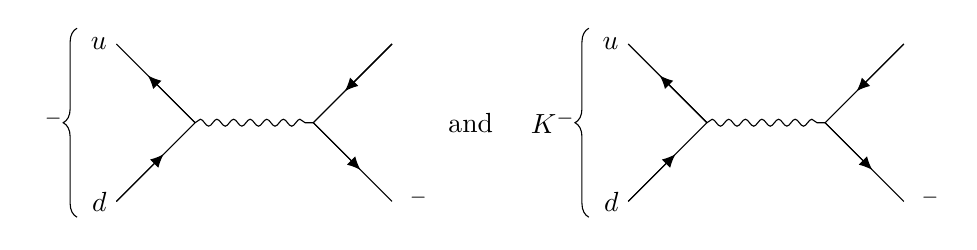
\begin{tikzpicture}[
            photon/.style={decoration={snake, amplitude=1.25, segment length=6}, decorate},
            >={Latex[width=1.5mm]},
            baseline=(current bounding box)
            ]
            \draw (0, 1) -- (1, 0) -- (0, -1);
            \draw[photon] (1, 0) -- (2.5, 0);
            \draw (3.5, 1) -- (2.5, 0) -- (3.5, -1);
            \draw[->] (0, -1) -- ++ (0.6, 0.6);
            \draw[->] (1, 0) -- ++ (-0.6, 0.6);
            \draw[->] (2.5, 0) -- ++ (0.6, -0.6);
            \draw[->] (3.5, 1) -- ++ (-0.6, -0.6);
            \node[left] at (0, 1) {\APu};
            \node[left] at (0, -1) {\Pd};
            \node[right] at (3.5, 1) {\APnumu};
            \node[right] at (3.5, -1) {\Pmu};
            \draw[decoration={brace, mirror, amplitude=5}, decorate] (-0.5, 1.2) -- (-0.5, -1.2);
            \node[left] at (-0.55, 0) {\Ppim};
            \node at (4.5, 0) {and};
            \begin{scope}[xshift=6.5cm]
                \draw (0, 1) -- (1, 0) -- (0, -1);
                \draw[photon] (1, 0) -- (2.5, 0);
                \draw (3.5, 1) -- (2.5, 0) -- (3.5, -1);
                \draw[->] (0, -1) -- ++ (0.6, 0.6);
                \draw[->] (1, 0) -- ++ (-0.6, 0.6);
                \draw[->] (2.5, 0) -- ++ (0.6, -0.6);
                \draw[->] (3.5, 1) -- ++ (-0.6, -0.6);
                \node[left] at (0, 1) {\APu};
                \node[left] at (0, -1) {\Pd};
                \node[right] at (3.5, 1) {\APnumu};
                \node[right] at (3.5, -1) {\Pmu};
                \draw[decoration={brace, mirror, amplitude=5}, decorate] (-0.5, 1.2) -- (-0.5, -1.2);
                \node[left] at (-0.55, 0) {\PKm};
            \end{scope}
        \end{tikzpicture}
    \end{equation*}
    
    Observations of this show that \PKm{} decays less than \Ppim{} does, after accounting for kinematic differences.
    This is actually why the strange quark is called the strange quark, because kaons have a strangely long lifetime.
    The solution to this problem is to realise that the weak interaction is different for different types of quarks.
    That is, there is no \enquote{quark universality} as far as the weak force is concerned.
    
    The way that this is born out in the mathematics is to have two different types of quarks.
    There are mass eigenstates, which are the usual particles we think of, and there are weak eigenstates, which are the states which interact through the weak force.
    This was first hypothesised by Cabibbo in 1963 (10 years before the bottom and top quark were discovered).
    He posited that the weak eigenstates, \(\Pd'\) and \(\Ps'\), are related to the mass eigenstates, \(\Pd\) and \(\Ps\) by
    \begin{equation}
        \begin{pmatrix}
            \Pd'\\ \Ps'
        \end{pmatrix}
        =
        \begin{pmatrix}
            \cos \cabibboAngle & \sin \cabibboAngle\\
            -\sin \cabibboAngle & \cos \cabibboAngle\\
        \end{pmatrix}
        \begin{pmatrix}
            \Pd\\ \Ps
        \end{pmatrix}
        \approx
        \begin{pmatrix}
            0.974 & 0.225\\
            -0.225 & 0.974
        \end{pmatrix}
        \begin{pmatrix}
            \Pd\\ \Ps
        \end{pmatrix}
    \end{equation}
    where \(\cabibboAngle \approx 0.227\) is the \defineindex{Cabbibo angle}.
    
    This idea is generalised to three generations of quarks through the \defineindex{Cabibbo--Kobayashi--Maskawa matrix}, or the \defineindex{CKM matrix}\glossary[acronym]{CKM}{Cabibbo--Kobayashi--Maskawa} matrix,
    \begin{equation}
        V_{\symrm{CKM}} = 
        \begin{pmatrix}
            V_{\Pu\Pd} & V_{\Pu\Ps} & V_{\Pu\Pb} \\
            V_{\Pc\Pd} & V_{\Pc\Ps} & V_{\Pc\Pb} \\
            V_{\Pt\Pd} & V_{\Pt\Ps} & V_{\Pt\Pb}
        \end{pmatrix}
        ,
    \end{equation}
    which relates the weak eigenstates, \(\Pd'\), \(\Ps'\), and \(\Pb'\), to the mass eigenstates, \(\Pd\), \(\Ps\), and \(\Pb\), through
    \begin{equation}
        \begin{pmatrix}
            \Pd'\\ \Ps'\\ \Pb'
        \end{pmatrix}
        =
        \begin{pmatrix}
            V_{\Pu\Pd} & V_{\Pu\Ps} & V_{\Pu\Pb} \\
            V_{\Pc\Pd} & V_{\Pc\Ps} & V_{\Pc\Pb} \\
            V_{\Pt\Pd} & V_{\Pt\Ps} & V_{\Pt\Pb}
        \end{pmatrix}
        \begin{pmatrix}
            \Pd\\ \Ps\\ \Pb
        \end{pmatrix}
        .
    \end{equation}
    
    The way this works is an up quark can only couple with \(\Pd'\), a charm quark can only couple with \(\Ps'\), and a top quark can only couple with \(\Pb'\) via the weak force.
    However, each of these weak eigenstates is a linear combination of the usual mass eigenstates.
    The coupling with the weak eigenstate occurs as normal with the normal charged current weak interaction coupling of \(g_{\PW}/\sqrt{2}\).
    However, we can expand this in a series of interactions involving the mass eigenstates, with the vertex term modified by a component of the CKM matrix.
    This modification is done by following the fermion line backwards.
    If we encounter \(\Pu\) then \(\Pd\), for example, then we multiply the vertex term by \(V_{\Pu\Pd}\), if instead we encounter \(\Pd\) then \(\Pu\) we multiply by \(V_{\Pu\Pd}^*\):
    \begin{equation}
        \tikzsetnextfilename{fd-W-boson-quark-vertex}
        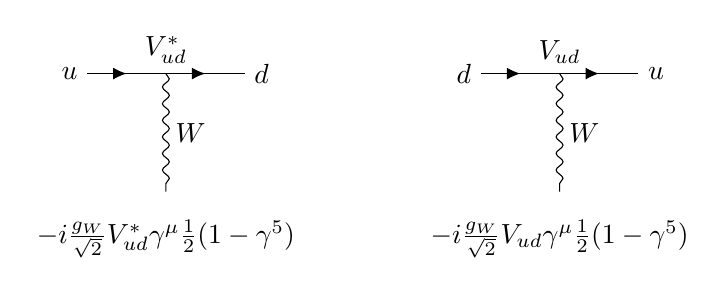
\begin{tikzpicture}[
            baseline=(q.base),
            photon/.style={decoration={snake, amplitude=1.25, segment length=6}, decorate},
            >={Latex[width=1.5mm]}
            ]
            \draw (0, 0) node (q) [left] {\Pu} -- (2, 0) node [right] {\Pd};
            \draw[->] (0, 0) -- (0.5, 0);
            \draw[->] (1, 0) node [above] {\(V_{\Pu\Pd}^*\)} -- (1.5, 0);
            \draw[photon] (1, 0) -- (1, -1.5) node [midway, right] {\PW};
            \node at (1, -2.1) {\(-i\frac{g_{\PW}}{\sqrt{2}} V_{\Pu\Pd}^* \gamma^\mu \frac{1}{2} (1 - \gamma^5)\)};
            \begin{scope}[xshift=5cm]
                \draw (0, 0) node (q) [left] {\Pd} -- (2, 0) node [right] {\Pu};
                \draw[->] (0, 0) -- (0.5, 0);
                \draw[->] (1, 0) node [above] {\(V_{\Pu\Pd}\)} -- (1.5, 0);
                \draw[photon] (1, 0) -- (1, -1.5) node [midway, right] {\PW};
                \node at (1, -2.1) {\(-i\frac{g_{\PW}}{\sqrt{2}} V_{\Pu\Pd} \gamma^\mu \frac{1}{2} (1 - \gamma^5)\)};
            \end{scope}
        \end{tikzpicture}
    \end{equation}
    We can decompose a vertex involving mass eigenstates into a sum of weak eigenstates:
    \begin{equation*}
        \tikzsetnextfilename{fd-CKM-modified-beta-decay}
        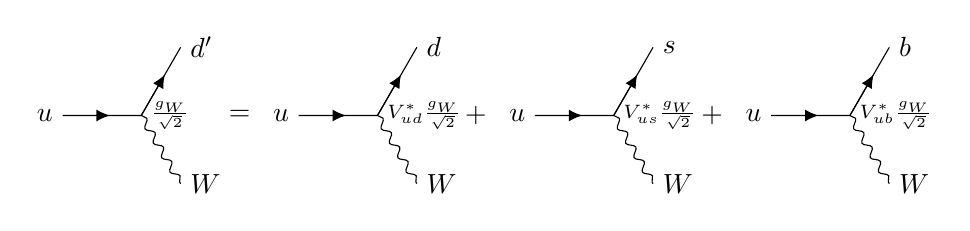
\begin{tikzpicture}[
            photon/.style={decoration={snake, amplitude=1.25, segment length=6}, decorate},
            >={Latex[width=1.5mm]},
            baseline=(current bounding box)
            ]
            \draw (-1, 0) node [left] {\Pu} -- (0, 0) -- (60:1) node [right] {\(\Pd'\)};
            \draw[photon] (0, 0) -- (-60:1) node [right] {\PW};
            \draw[->] (-1, 0) -- (-0.4, 0);
            \draw[->] (0, 0) -- (60:0.6);
            \node at (1.25, 0) {\(=\)};
            \node[right] at (0, 0) {\scriptsize\(\frac{g_{\PW}}{\sqrt{2}}\)};
            \begin{scope}[xshift=3cm]
                \draw (-1, 0) node [left] {\Pu} -- (0, 0) -- (60:1) node [right] {\Pd};
                \draw[photon] (0, 0) -- (-60:1) node [right] {\PW};
                \draw[->] (-1, 0) -- (-0.4, 0);
                \draw[->] (0, 0) -- (60:0.6);
                \node at (1.25, 0) {\(+\)};
                \node[right] at (0, 0) {\scriptsize\(V_{\Pu\Pd}^*\frac{g_{\PW}}{\sqrt{2}}\)};
            \end{scope}
            \begin{scope}[xshift=6cm]
                \draw (-1, 0) node [left] {\Pu} -- (0, 0) -- (60:1) node [right] {\Ps};
                \draw[photon] (0, 0) -- (-60:1) node [right] {\PW};
                \draw[->] (-1, 0) -- (-0.4, 0);
                \draw[->] (0, 0) -- (60:0.6);
                \node at (1.25, 0) {\(+\)};
                \node[right] at (0, 0) {\scriptsize\(V_{\Pu\Ps}^*\frac{g_{\PW}}{\sqrt{2}}\)};
            \end{scope}
            \begin{scope}[xshift=9cm]
                \draw (-1, 0) node [left] {\Pu} -- (0, 0) -- (60:1) node [right] {\Pb};
                \draw[photon] (0, 0) -- (-60:1) node [right] {\PW};
                \draw[->] (-1, 0) -- (-0.4, 0);
                \draw[->] (0, 0) -- (60:0.6);
                \node[right] at (0, 0) {\scriptsize\(V_{\Pu\Pb}^*\frac{g_{\PW}}{\sqrt{2}}\)};
            \end{scope}
        \end{tikzpicture}
    \end{equation*}
    
    Note that by convention the CKM matrix is defined as modifying the down-type quarks, and the up-type quarks are unaffected.
    The elements of the CKM matrix are complex constants.
    They aren't predicted by the standard model, instead they have to be determined from experiments, much like the particle masses.
    The CKM matrix is unitary.
    
    The result of all of this is a modified interaction, and hence a modified vertex term.
    For a charged current weak interaction involving a quarks, which for the sake of example we take to be up and down, the vertex term is one of
    \begin{equation}
        -i \frac{g_{\PW}}{\sqrt{2}} V_{\Pu\Pd} \gamma^\mu \frac{1}{2}(1 - \gamma^5), \qqor -i\frac{g_{\PW}}{\sqrt{2}} V_{\Pu\Pd}^* \gamma^\mu \frac{1}{2}(1 - \gamma^5).
    \end{equation}
    
    Recent measurements put the absolute values of the elements of the CKM matrix at
    \begingroup
    \def\arraystretch{1.4}
    \begin{equation}
        \left(
        \begin{array}{@{}r@{}lr@{}lr@{}l@{}}
            0.97435 & {} \pm 0.00016 & 0.22599 & {} \pm 0.00067 & 0.00369 & {} \pm 0.00011\\
            0.22486 & {} \pm 0.00067 & 0.97349 & {} \pm 0.00016 & 0.04182 & {} \mathbin{\substack{+0.00085\\ -0.00074}} {}\\
            0.00857 & {} \mathbin{\substack{+0.00020\\ -0.00018}} {} & 0.04110 & {} \mathbin{\substack{+0.00083\\ -0.00072}} {} &  0.999118 & {}  \mathbin{\substack{+ 0.000031\\ - 0.000036}} {}
        \end{array}
        \right)
        .
    \end{equation}
    \endgroup
    Notice that the values are largest on the leading diagonal, smaller either side of the diagonal, and smallest furthest from the diagonal.
    What this means is that the weak eigenstates are mostly formed from the equivalent mass eigenstate, so \(\Pd'\) is mostly \(\Pd\), a little bit from the quark in neighbouring generations, so \(\Pd'\) is a little bit of \(\Ps\), and barely any from further generations, so the contribution of \(\Pb\) to \(\Pd\) is tiny.
    Here's a plot which better displays this, full black represents a value of 1 and full white a value of 0:
    \begin{equation}
        \tikzsetnextfilename{CKM}
        
\begin{tikzpicture}[baseline=(current bounding box)]
            \fill[black!1!white] (0, 0) rectangle (0.5, 0.5);
            \fill[black!4!white] (0.5, 0) rectangle (1, 0.5);
            \fill[black!100!white] (1, 0) rectangle (1.5, 0.5);
            \fill[black!22!white] (0, 0.5) rectangle (0.5, 1);
            \fill[black!97!white] (0.5, 0.5) rectangle (1, 1);
            \fill[black!4!white] (1, 0.5) rectangle (1.5, 1);
            \fill[black!97!white] (0, 1) rectangle (0.5, 1.5);
            \fill[black!23!white] (0.5, 1) rectangle (1, 1.5);
            \fill[black!0!white] (1, 1) rectangle (1.5, 1.5);
        \end{tikzpicture}
    \end{equation}
    
    \chapter{Symmetry in Weak Interactions}
    \section{Kaons}
    There are two neutral kaons, \(\PKzero\) and \(\APKzero\).
    These have quark content \(\Pd\APs\) and \(\Ps\APd\) respectively.
    It is possible for the two neutral kaons to \enquote{mix}, that is turn into each other, through the interactions
    \begin{equation}
        \tikzsetnextfilename{fd-Kzero-mixing-1}
        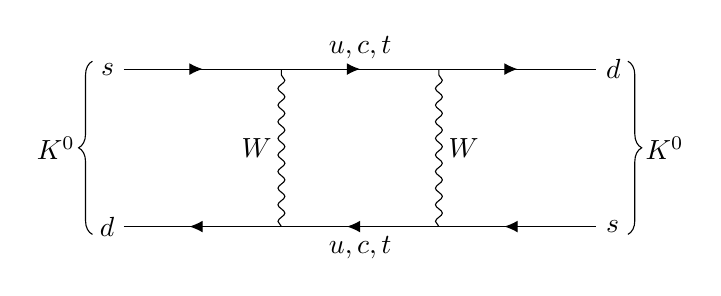
\begin{tikzpicture}[
            baseline=(current bounding box),
            photon/.style={decoration={snake, amplitude=1.25, segment length=6}, decorate},
            >={Latex[width=1.5mm]}
            ]
            \draw (0, 0) node [left] {\APd} -- (6, 0) node [right] {\APs};
            \draw (0, 2) node [left] {\Ps} -- (6, 2) node [right] {\Pd};
            \draw[photon] (2, 0) -- (2, 2) node [midway, left] {\PW};
            \draw[photon] (4, 0) -- (4, 2) node [midway, right] {\PW};
            \draw[-<] (0, 0) -- (1, 0);
            \draw[-<] (2, 0) -- (3, 0) node [below] {\(\APu, \APc, \APt\)};
            \draw[-<] (4, 0) -- (5, 0);
            \draw[->] (0, 2) -- (1, 2);
            \draw[->] (2, 2) -- (3, 2) node [above] {\(\Pu, \Pc, \Pt\)};
            \draw[->] (4, 2) -- (5, 2);
            \draw[decoration={brace, amplitude=5}, decorate] (-0.4, -0.1) -- (-0.4, 2.1) node [midway, left, xshift=-0.1cm] {\APKzero};
            \draw[decoration={brace, amplitude=5, mirror}, decorate] (6.4, -0.1) -- (6.4, 2.1) node [midway, right, xshift=0.1cm] {\PKzero};
        \end{tikzpicture}
    \end{equation}
    and
    \begin{equation}
        \tikzsetnextfilename{fd-Kzero-mixing-2}
        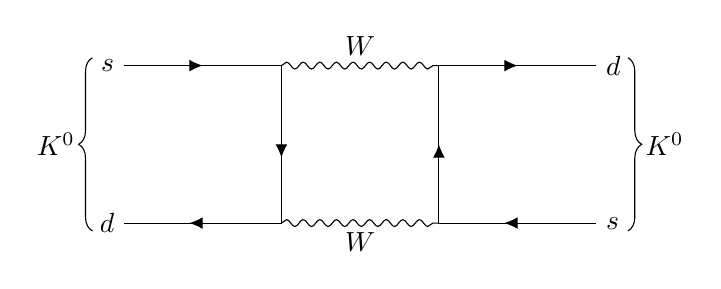
\begin{tikzpicture}[
            baseline=(current bounding box),
            photon/.style={decoration={snake, amplitude=1.25, segment length=6}, decorate},
            >={Latex[width=1.5mm]}
            ]
            \draw (0, 0) node [left] {\APd} -- (2, 0) -- (2, 2) -- (0, 2) node [left] {\Ps};
            \draw (6, 0) node [right] {\APs} -- (4, 0) -- (4, 2) -- (6, 2) node [right] {\Pd};
            \draw[photon] (2, 0) -- (4, 0) node [midway, below] {\PW};
            \draw[photon] (2, 2) -- (4, 2) node [midway, above] {\PW};
            \draw[-<] (0, 0) -- (1, 0);
            \draw[-<] (4, 0) -- (5, 0);
            \draw[-<] (2, 0) -- (2, 1);
            \draw[->] (0, 2) -- (1, 2);
            \draw[->] (4, 2) -- (5, 2);
            \draw[->] (4, 0) -- (4, 1);
            \draw[decoration={brace, amplitude=5}, decorate] (-0.4, -0.1) -- (-0.4, 2.1) node [midway, left, xshift=-0.1cm] {\APKzero};
            \draw[decoration={brace, amplitude=5, mirror}, decorate] (6.4, -0.1) -- (6.4, 2.1) node [midway, right, xshift=0.1cm] {\PKzero};
        \end{tikzpicture}
    \end{equation}
    These process can also happen in the opposite direction.
    
    Charge conjugation takes particles to their antiparticles, so it takes \(\Pd\APs\) to \(\Ps\APd\), so it takes \(\PKzero\) to \(\APKzero\).
    That is,
    \begin{equation}
        \chargeConjugation \ket{\PKzero} = \ket{\APKzero}, \qqand \chargeConjugation \ket{\APKzero} = \ket{\PKzero}.
    \end{equation}

    The action of parity on neutral kaons is less clear.
    It turns out that both neutral kaons are pseudoscalars, they have \(J^P = 0^-\) (that is spin, \(J\), zero and parity, \(P\), \(-1\)).
    Hence,
    \begin{equation}
        \parity \ket{\PKzero} = -\ket{\PKzero}, \qqand \parity \ket{\APKzero} = -\ket{\APKzero}.
    \end{equation}
    
    Combining these we see that the neutral kaons are not eigenstates of the combined \(\chargeConjugation\parity\) operator:
    \begin{equation}
        \chargeConjugation\parity \ket{\PKzero} = -\ket{\APKzero}, \qqand \chargeConjugation\parity \ket{\APKzero} = -\ket{\PKzero}.
    \end{equation}
    
    In order to form eigenstates of the combined \(\chargeConjugation\parity\) operator we can take linear combinations of the neutral kaons, defining
    \begin{align}
        \ket{\PK_1} &\coloneqq \frac{1}{\sqrt{2}} (\ket{\PKzero} - \ket{\APKzero}),\\
        \ket{\PK_2} &\coloneqq \frac{1}{\sqrt{2}} (\ket{\PKzero} + \ket{\APKzero}).
    \end{align}
    Then
    \begin{equation}
        \chargeConjugation\parity\ket{\PK_1} = +\ket{\PK_1}, \qqand \chargeConjugation\parity\ket{\PK_2} = -\ket{\PK_1},
    \end{equation}
    so \(\ket{\PK_1}\) and \(\ket{\PK_2}\) are eigenstates of \(\chargeConjugation\parity\) with eigenvalues \(+1\) and \(-1\) respectively.
    Note that by construction \(\ket{\PK_1}\) and \(\ket{\PK_2}\) are orthogonal, so we can reconstruct \(\ket{\PKzero}\) and \(\ket{\APKzero}\) as a linear combination of \(\ket{\PK_1}\) and \(\ket{\PK_2}\).
    We refer to \(\PKzero\) and \(\APKzero\) as strong eigenstates, since they have definite quark content so their interactions through the strong force don't change them.
    
    When it comes to decays it is possible for neutral kaons to decay into either two or three pions.
    The three pions have a \(\chargeConjugation\parity\) eigenvalue of \(-1\), whereas the two pions have a \(\chargeConjugation\parity\) eigenvalue of \(+1\).
    This suggests that it is not the \(\ket{\PK_1}\) or \(\ket{\PK_2}\) states that decay, but a linear combination of them:
    \begin{align}
        \ket{\PKshort} &\coloneqq \frac{1}{\sqrt{1 + \abs{\varepsilon}^2}} (\ket{\PK_1} + \varepsilon\ket{\PK_2}),\\
        \ket{\PKlong} &\coloneqq \frac{1}{\sqrt{1 + \abs{\varepsilon}^2}} (\ket{\PK_2} + \varepsilon\ket{\PK_1}),
    \end{align}
    where \(\varepsilon \in \complex\) with \(\abs{\varepsilon} \approx \num{2e-3}\).
    The \(\symrm{S}\) and \(\symrm{L}\) stand for short and long respectively, and we read \(\PKshort\) as \enquote{\(\PK\) short} and \(\PKlong\) as \enquote{\(\PK\) long}.
    These names correspond to the observation that \(\ket{\PKlong}\) has a longer half life (\(\tau(\PKlong) \approx \qty{5e-8}{\second}\)) than \(\ket{\PKshort}\) (\(\tau(\PKshort) \approx \qty{9e-11}{\second}\)).
    
    We interpret a decay into 2 pions as occurring due to the kaon being in state \(\ket{\PK_1}\), since this state and a pair of pions both have \(\chargeConjugation\parity\) eigenvalue \(+1\).
    Similarly a decay into 3 pions occurs due to the kaon being in state \(\ket{\PK_2}\), since this state a nd a triplet of pions both have \(\chargeConjugation\parity\) eigenvalue \(-1\).
    
    Since the decay eigenstates, \(\PKlong\) and \(\PKshort\), are not \(\chargeConjugation\parity\) eigenstates we see that \(\chargeConjugation\parity\) symmetry is violated in the weak interaction.
    The amount of \(\chargeConjugation\parity\) violation in neutral kaon mixing is small, on the order of \(\num{2e-3}\), corresponding to the branching ratio for \(\PKlong\) to decay to a pair of pions, since most measurements of \(\PKlong\) will measure the \(\chargeConjugation\parity\) eigenvalue to be \(-1\), since it's mostly formed from \(\ket{\PK_2}\), and the pair of pions has \(\chargeConjugation\parity\) eigenvalue \(+1\).
    
    Now consider the mixing diagrams from the start of this section.
    Going one way along the lines we get vertices with \(V_{\Pq\Pq}\), and going the other way we get \(V_{\Pq\Pq}^*\).
    This makes the two directions, \(\PKzero \to \APKzero\) and \(\APKzero \to \PKzero\), antisymmetric.
    It works out so that we get slightly more decays \(\APKzero \to \PKzero\) than \(\PKzero \to \APKzero\).
    
    We see very similar phenomena with other neutral mesons, including the \(\PB\) mesons, \(\PBzerodown\) (\(\Pd\APb\)), \(\APBzerodown\) (\(\Pb\APd\)), \(\PBzerostrange\) (\(\Ps\APb\)), and \(\APBzerostrange\) (\(\Pb\APs\)).
    As well as more recent observations of this with some charm mesons such as \(\PDzero\) (\(\Pc\APd\)) and \(\APDzero\) (\(\Pd\APc\)).
    
    We also observe \(\chargeConjugation\parity\) violation in decays involving the weak force, for example,
    \begin{equation}
        \Gamma(\PBzerodown \to \PKp \Ppim) \ne \Gamma(\APBzerodown \to \PKm \Ppip).
    \end{equation}
    
    \section{\texorpdfstring{\(\chargeConjugation\parity\)}{CP} Violation in the Early Universe}
    In the early universe the thermal energy, \(\boltzmann T\), was large compared to hadron masses.
    This allowed for processes like \(\Pphoton\Pphoton \to \Pp\APp\), producing protons and antiprotons in equal number.
    After a while the universe expanded and cooled, and proton production stopped.
    At this point we think that the fraction of baryons to photons was the same as the fraction of antibaryons to photons,
    \begin{equation}
        \frac{n_{\symrm{B}}}{n_{\Pphoton}} = \frac{n_{\APantiparticle{\symrm{B}}}}{n_{\Pphoton}} \approx 10^{-18}.
    \end{equation}
    However, measurements now give the result
    \begin{equation}
        \frac{n_{\symrm{B}}(\text{today})}{n_{\Pphoton}} = \frac{n_{\symrm{B}} - n_{\APantiparticle{\symrm{B}}}}{n_{\Pphoton}} \approx 10^{-9}.
    \end{equation}
    This means there is an antisymmetry between baryons and antibaryons, to get the universe we see today the universe must have started with \(10^{9} + 1\) baryons for every \(10^9\) baryons.
    This initial asymmetry requires three conditions:
    \begin{itemize}
        \item Baryon number, \(n_{\symrm{B}} - n_{\APantiparticle{\symrm{B}}}\), is not conserved.
        \item Departure from thermal equilibrium, where baryon number violating processes are balanced by the inverse process.
        \item \(\chargeConjugation\) and \(\chargeConjugation\parity\) violation, if \(\chargeConjugation\parity\) is conserved then for every process producing baryons there would be an equivalent process producing antibaryons.
    \end{itemize}
    
    We've seen that there is \(\chargeConjugation\parity\) violation in the quark sector, such as with neutral kaon mixing.
    However, the effect of this is \emph{not} large enough to account for the matter/antimatter asymmetry.
    One possible solution would be a similar violation in the neutrino sector.
    \begin{openquestion}
        Is there \(\chargeConjugation\parity\) violation in weak interactions involving neutrinos?
        If there is is there enough to account for the matter/antimatter asymmetry of the universe?
    \end{openquestion}
    
    \section{Weak Isospin}
    \begin{rmk}
        We will start using a particle's symbol to refer to it's spinor wave function, since the flavour of spinors now becomes important.
        For example, \(\Penominus_{\Left}\) corresponds to a left handed chiral electron spinor, \(\diracadjoint{\Penominus}_{\Left}\) corresponds to a left handed chiral electron adjoint spinor (not to a left handed positron spinor), \(\upnu_{\symrm{e}\Left}\) corresponds to a left handed chiral neutrino spinor, and so on.
    \end{rmk}
    We've seen that electromagnetic interactions can be understood through a \(\unitary(1)\) gauge symmetry involving a gauge boson, \(A_\mu\), the photon.
    Similarly the strong interactions can be understood through a \(\specialUnitary(3)\) gauge symmetry involving eight gauge bosons, \(G^a_\mu\), the gluons.
    We can similarly understand weak interactions through a \(\specialUnitary(2)\) gauge symmetry involving three gauge bosons, \(W_\mu^k\), for \(k = 1, 2, 3\), which we call the \(\PW\) bosons.
    These are \emph{not} the \(\PWpm\) bosons.
    
    The symmetry group here,
    \begin{equation}
        \specialUnitary(2) \coloneqq \{U \in \matrices{2}{\complex} \mid U^\hermit U = 1 \text{ and } \det U = 1\},
    \end{equation}
    is the special unitary group of \(2 \times 2\) matrices.
    In this context we often call this symmetry group \(\specialUnitary(2)_{\Left}\), probably to distinguish it from the \(\specialUnitary(2)\) appearing when we discuss spin.
    
    As with QED and QCD we have a \enquote{charge} measuring the coupling of the gauge bosons to particles.
    In weak interactions we call this \defineindex{weak isospin}\footnote{the spin part of this name is due to the fact that \(\specialUnitary(2)\) also describes spin, and so there are a lot of mathematical analogies to be drawn between spin and weak isospin.}
    Much like spin we describe weak isospin with the total weak isospin, \(I_{\PW}\), and the third component of the weak isospin, \(I_{\PW}^{(3)}\).
    
    We define \define{weak isospin doublets}\index{weak isospin!doublet} containing two fermion spinor flavours which are coupled by \(\PWpm\).
    For example, an interaction with \(\PWpm\) can couple electrons and electron neutrinos, so these form a doublet,
    \begin{equation}
        \begin{pmatrix}
            {\Pnue}_{\Left}\\ \Penominus_{\Left}.
        \end{pmatrix}
    \end{equation}
    Since the \(\PWpm\) bosons only interact with left handed fermions we only consider the left handed fermions in these doublets.
    The total weak isospin of these doublets is\footnote{i.e., these doublets are in the \(\rep{2}\) representation of \(\specialUnitary(2)\).} \(I_{\PW} = +1/2\).
    The upper component has\footnote{i.e., the two components are the two basis vectors of \(\rep{2}\).} \(I_{\PW}^{(3)} = +1/2\) and the lower component has \(I_{\PW}^{(3)} = -1/2\).
    
    We can do exactly the same for the other fermions, all following the same pattern, just note that \(\PWpm\) couple \(\Pu\) to \(\Pd'\) and so on.
    We get all the weak isospin doublets:
    \begin{equation}
        \begin{pmatrix}
            {\upnu}_{\symrm{e}\Left}\\ \Penominus_{\Left}
        \end{pmatrix}
        , \quad
        \begin{pmatrix}
            {\upnu}_{\upmu\Left}\\ \Pmunominus_{\Left}
        \end{pmatrix}
        , \quad
        \begin{pmatrix}
            {\upnu}_{\uptau\Left}\\ \Ptaunominus_{\Left}
        \end{pmatrix}
        , \quad
        \begin{pmatrix}
            \Pu\\ \Pd'
        \end{pmatrix}
        , \quad
        \begin{pmatrix}
            \Pu\\ \Pd'
        \end{pmatrix}
        , \quad
        \begin{pmatrix}
            \Pc\\ \Ps'
        \end{pmatrix}
        , \quad
        \begin{pmatrix}
            \Pt\\ \Pb'
        \end{pmatrix}
        .
    \end{equation}
    
    The charged fermions also have right handed chiral components.
    These are in weak isospin singlets\footnote{i.e., these singlets are in the \(\rep{1}\) trivial representation of \(\specialUnitary(2)\).}, with \(I_{\PW} = 0\) and \(I_{\PW}^{(3)} = 0\),
    \begin{equation}
        \Penominus_{\Right}, \quad \Pmunominus_{\Right}, \quad \Ptaunominus_{\Right}, \quad \Pu_{\Right}, \quad \Pc_{\Right}, \quad \Pt_{\Right}, \quad \Pd_{\Right}, \quad \Ps_{\Right}, \qand \Pb_{\Right}.
    \end{equation}
    
    As with the other gauge theories we've seen the weak interaction gauge theory results in a modified Dirac equation:
    \begin{align}
        i\gamma^\mu \left( \partial_\mu + ig_{\PW} \frac{1}{2}\sigma_k W_\mu^k \right) \varphi - m\varphi = 0,\\
        i\left( \slashed{\partial} + ig_{\PW} \frac{1}{2}\sigma_k \slashed{W}^k \right) \varphi - m\varphi = 0,
    \end{align}
    where \(\sigma_i\) are the Pauli spin matrices\footnote{the generators of \(\specialUnitaryLie(2)\) in the \(\rep{2}\) representation are \(\sigma_i/2\).},
    \begin{equation}
        \sigma_1 = 
        \begin{pmatrix}
            0 & 1\\
            1 & 0
        \end{pmatrix}
        , \sigma_2 = 
        \begin{pmatrix}
            0 & -i\\
            i & 0
        \end{pmatrix}
        , \qqand \sigma_3 = 
        \begin{pmatrix}
            1 & 0\\
            0 & -1
        \end{pmatrix}
        .
    \end{equation}
    
    To go with each \(\PW\) boson we get three left handed weak fermion currents:
    \begin{equation}
        j_k^\mu = \frac{g_{\PW}}{2} \diracadjoint{\varphi}_{\Left} \gamma^\mu \sigma_k \varphi_{\Left}
    \end{equation}
    where \(\varphi_{\Left}\) is a weak isospin doublet, and \(\diracadjoint{\varphi}_{\Left}\) its adjoint, for example,
    \begin{equation}
        \varphi_{\Left} = 
        \begin{pmatrix}
            {\upnu}_{\symrm{e}\Left}\\ \Penominus_{\Left}
        \end{pmatrix}
        , \qqand
        \diracadjoint{\varphi}_{\Left} = 
        \begin{pmatrix}
            \diracadjoint{\upnu}_{\symrm{e}\Left} & \diracadjoint{\Penominus}_{\Left}
        \end{pmatrix}
        .
    \end{equation}
    
    The \(\PWpm\) charged currents correspond to linear combinations of these currents\footnote{i.e., \(\PWpm\) are raising and lowering operators in \(\specialUnitaryLie(2)\).}
    \begin{equation}
        j_{\pm}^\mu = \frac{1}{\sqrt{2}} (j_1^\mu \pm i j_2^\mu) = \frac{g_{\PW}}{\sqrt{2}} \diracadjoint{\varphi}_{\Left} \gamma^\mu \frac{1}{2}(\sigma_1 \pm i \sigma_2) \varphi_{\Left}.
    \end{equation}
    
    We can define
    \begin{equation}
        \sigma_+ = \frac{1}{2}(\sigma_1 + i\sigma_2) = 
        \begin{pmatrix}
            0 & 1\\
            0 & 0
        \end{pmatrix}
        , \qqand \sigma_- = \frac{1}{2}(\sigma_1 - i\sigma_2) = 
        \begin{pmatrix}
            0 & 0\\
            1 & 0
        \end{pmatrix}
        .
    \end{equation}
    Then we find that the \(\PWp\) current for an electron/neutrino doublet is
    \begin{align}
        j_+^\mu &= \frac{g_{\PW}}{\sqrt{2}} \diracadjoint{\varphi}_{\Left} \gamma^\mu \sigma_+ \varphi_{\Left}\\
        &= \frac{g_{\PW}}{\sqrt{2}}
        \begin{pmatrix}
            \diracadjoint{\upnu}_{\symrm{e}\Left} & \diracadjoint{\Penominus}_{\Left}
        \end{pmatrix}
        \gamma^\mu 
        \begin{pmatrix}
            0 & 1\\
            0 & 0
        \end{pmatrix}
        \begin{pmatrix}
            \upnu_{\symrm{e}\Left}\\
            \Penominus_{\Left}
        \end{pmatrix}
        \\
        &= \frac{g_{\PW}}{\sqrt{2}} \diracadjoint{\upnu}_{\symrm{e}\Left} \gamma^\mu \Penominus_{\Left}\\
        &= \frac{g_{\PW}}{\sqrt{2}} \diracadjoint{\upnu}_{\symrm{e}} \gamma^\mu\frac{1}{2} (1 - \gamma^5) \Penominus.
    \end{align}
    So we see that this describes an interaction with a vertex where a left handed electron emits a \(\PWp\) and becomes a left handed electron neutrino.
    
    Similarly the \(\PWm\) current describes a left handed electron neutrino emitting a \(\PWm\) and becoming a left handed electron.
    
    There is a third component of the \(\PW\) bosons which we haven't accounted for but is predicted by the \(\specialUnitary(2)\) symmetry.
    The third current for an electron/neutrino doublet is
    \begin{align}
        j_3^\mu &= \frac{g_{\PW}}{2} \diracadjoint{\varphi}_{\Left}\gamma^\mu \sigma_3\varphi_{\Left}\\
        &= \frac{g_{\PW}}{2} 
        \begin{pmatrix}
            \diracadjoint{\upnu}_{\symrm{e}\Left} & \diracadjoint{\Penominus}_{\Left}
        \end{pmatrix}
        \gamma^\mu
        \begin{pmatrix}
            1 & 0\\
            0 & -1
        \end{pmatrix}
        \begin{pmatrix}
            \upnu_{\symrm{e}\Left}\\
            \Penominus_{\Left}
        \end{pmatrix}
        \\
        &= \frac{g_{\PW}}{2} \diracadjoint{\upnu}_{\symrm{e}\Left} \gamma^\mu \upnu_{\symrm{e}\Left} - \frac{g_{\PW}}{2} \diracadjoint{\Penominus}_{\Left} \gamma^\mu \Penominus_{\Left}.
    \end{align}
    So, this corresponds to an electron or neutrino going along and emitting a \(\PW^{(3)}\) boson without a flavour change.
    \begin{wrn}
        \(\PW^{(3)}\) is \emph{not} the \(\PZ\) boson, but it is related to it, as we'll see in the next chapter.
    \end{wrn}
    The general fermion current for this is
    \begin{equation}
        j_3^\mu = I_{\PW}^{(3)} g_{\PW} \diracadjoint{\Pf} \gamma^\mu \frac{1}{2}(1 - \gamma^5)\Pf.
    \end{equation}

    \chapter{Electroweak Unification}
    \section{Electroweak Theory}
    \define{Electroweak theory}\index{electroweak theory} is the quantum field theory combing electromagnetic and weak interactions.
    As such we expect it to reproduce QED when we take out the components corresponding to weak interactions, and we'll use this as a guiding principle for the development of electroweak theory.
    Electroweak unification proposes a new \(\unitary(1)\) symmetry with a boson \(B_\mu\) which couples to particles carrying \defineindex{weak hypercharge}, \(Y\), with coupling constant \(g'\)\footnote{compare to QED: a \(\unitary(1)\) symmetry with a boson \(A_\mu\) which couples to particles carrying electric charge, \(Q\), with coupling constant \(e\).}.
    We then modify the Dirac equation to have an extra term\footnote{compare to the extra term in QED: \(ieQ_{\Pf}\slashed{A}\psi\).}:
    \begin{equation}
        i\left( \slashed{\partial} + i\frac{Y}{2}\slashed{B} \right)\psi - m\psi = 0.
    \end{equation}
    Note that the the weak hypercharge can be different for left and right handed fermions.
    
    The full electroweak theory is then the gauge theory of \(\specialUnitary(2)_{\Left} \times U(1)_{Y}\).
    The subscript \(Y\) here is to distinguish this from the \(U(1)_{\symrm{em}}\) of QED.
    
    In the electroweak model the photon and \PZ{} boson are linear combinations of the \(B_\mu\) and \(W^{(3)}_\mu\) bosons:
    \begin{align}
        A_\mu &= +B_\mu \cos\vartheta_{\PW} + W_\mu^{(3)} \sin\vartheta,\\
        Z_\mu &= -B_\mu \sin\vartheta_{\PW} + W_\mu^{(3)} \cos\vartheta.
    \end{align}
    This combination is parametrised by the \defineindex{weak mixing angle} \(\vartheta_{\PW}\).
    Note that by construction \(A_\mu\) and \(Z_\mu\) are an orthogonal combination of \(B_\mu\) and \(W_\mu\).
    As before \(\PWpm\) are given by \(W^{(1)}_\mu \pm i W^{(2)}_\mu\).
    
    The fermion currents are then
    \begin{align}
        j^\mu_{\symrm{em}} &= +j_Y^\mu \cos\vartheta_{\PW} + j_3^\mu\sin\vartheta_{\PW},\\
        j_{\PZ}^\mu &= -j_Y^\mu\sin\vartheta_{\PW} + j_3^\mu\cos\vartheta_{\PW}.
    \end{align}
    Here \(j^\mu_3\) is the current of the \(\PW^{(3)}\) boson as discussed in the previous chapter, and \(j_Y^{\mu}\) is the current associated with \(B_\mu\), given, for the electron/neutrino doublet, by
    \begin{equation*}
        j_Y^\mu = \frac{1}{2}g' Y_{\Penominus_{\Left}} \diracadjoint{\Penominus}_{\Left} \gamma^\mu \Penominus_{\Left} + \frac{1}{2}g' Y_{\Penominus_{\Right}} \diracadjoint{\Penominus}_{\Right} \gamma^\mu \Penominus_{\Right} + \frac{1}{2} g' Y_{\upnu_{\symrm{e}\Left}} \diracadjoint{\upnu}_{\symrm{e}\Left} \gamma^\mu \upnu_{\symrm{e}\Left} + \frac{1}{2} g' Y_{\upnu_{\symrm{e}\Right}} \diracadjoint{\upnu}_{\symrm{e}\Right} \gamma^\mu \upnu_{\symrm{e}\Right}.
    \end{equation*}
    Here \(Y_{\Penominus_{\Left}}\) is the weak hypercharge of the left handed electron and so on.
    
    \section{Coupling to Photons}
    We demand that the couplings between a photon and a fermion is given by the electric charge of the fermion, as is the case in QED.
    Writing out the electromagnetic fermion current for an electron/neutrino doublet we have
    \begin{align}
        j_{\symrm{em}}^{\mu} &= j_Y^\mu \cos\vartheta_{\PW} + j_3^\mu \sin\vartheta_{\PW}\\
        &= \frac{1}{2}g' (Y_{\Penominus_{\Left}} \diracadjoint{\Penominus}_{\Left} \gamma^\mu \Penominus_{\Left} + Y_{\Penominus_{\Right}} \diracadjoint{\Penominus}_{\Right} \gamma^\mu \Penominus_{\Right} + Y_{\upnu_{\symrm{e}\Left}} \diracadjoint{\upnu}_{\symrm{e}\Left} \gamma^\mu \upnu_{\symrm{e}\Left} + Y_{\upnu_{\symrm{e}\Right}} \diracadjoint{\upnu}_{\symrm{e}\Right} \gamma^\mu \upnu_{\symrm{e}\Right})\cos\vartheta_{\PW}\\
        &\qquad \frac{g_{\PW}}{2}(I_{\PW \, \upnu_{\symrm{e}\Left}}^{(3)} \diracadjoint{\upnu}_{\Left} \gamma^\mu \upnu_{\Left} + I_{\PW \, \Penominus_{\Left}}^{(3)} \diracadjoint{\Penominus}_{\Left} \gamma^\mu \Penominus_{\Left}) \sin\vartheta_{\PW}
    \end{align}
    where \(I_{\PW \, \upnu_{\symrm{e}\Left}}^{(3)}\) is the third component of the weak isospin of the left handed electron neutrino and so on.
    
    Comparing this with the expected current for the electron, with charge \(Q_{\Penominus}e\), and neutrino with charge \(0\) for both the left and right handed particles we demand the following hold:
    \begin{align}
        Q_{\Penominus}e &= \frac{g'}{2} Y_{\Penominus_{\Left}} \cos\vartheta_{\PW} + \frac{g_{\PW}}{2} I_{\PW \, \symrm{e}_{\Left}}^{(3)} \sin\vartheta_{\PW},\\
        Q_{\Penominus}e &= \frac{g'}{2} Y_{\Penominus_{\Right}} \cos\vartheta_{\PW},\\
        0 &= \frac{g'}{2} Y_{\upnu_{\Left}} \cos\vartheta_{\PW} + \frac{g_{\PW}}{2} I_{\PW \, \upnu_{\symrm{e}\Left}} \sin \vartheta_{\PW},\\
        0 &= \frac{g'}{2} Y_{\upnu_{\Right}} \cos\vartheta_{\PW}.
    \end{align}
    Using \(I_{\PW \, \symrm{e}_{\Left}}^{(3)} = -1/2\) and \(I_{\PW \, \upnu_{\symrm{e}\Left}}^{(3)} = 1/2\) we find that
    \begin{equation}
        e = g_{\PW} \sin\vartheta_{\PW} = g'\cos\vartheta_{\PW}, \qqand Y = 2(Q - I_{\PW}^{(3)}).
    \end{equation}
    Experimentally we know that
    \begin{equation}
        \sin^2 \vartheta_{\PW} = \num{0.23146(12)}.
    \end{equation}
    
    \section{Coupling to \texorpdfstring{\PZ}{Z} Bosons}
    After defining the parameters in electroweak theory such that we get the same results for photon coupling as QED the coupling for the \PZ{} boson is fully specified.
    The \PZ{} boson current for a fermion of flavour \(\Pf\) with left and right handed chiral spinor states \(u_{\Left}\) and \(u_{\Right}\) such that the left handed spinors have third component of weak isospin \(I_{\PW}^{(3)}\) is
    \begin{equation}
        j_{\PZ}^\mu = -\frac{1}{2}g' \sin\vartheta_{\PW} [Y_{\Pf_{\Left}} \diracadjoint{u}_{\Left} \gamma^\mu u_{\Left} + Y_{\Pf_{\Right}} \diracadjoint{u}_{\Right} \gamma^\mu u_{\Right}] + I_{\PW}^{(3)} g_{\PW} \cos\vartheta_{\PW} [\diracadjoint{u}_{\Left} \gamma^\mu u_{\Left}].
    \end{equation}
    We can rewrite this as
    \begin{align}
        j_{\PZ}^{\mu} &= g_{\PW}\left[ -(Q_{\Pf} - I_{\PW}^{(3)}) \frac{\sin^2\vartheta_{\PW}}{\cos\vartheta_{\PW}} + I_{\PW}^{(3)}\cos\vartheta_{\PW} \right]\diracadjoint{u}_{\Left}\gamma^\mu u_{\Left}\\
        &\qquad\qquad - g_{\PW} \left[ \frac{\sin^2\vartheta_{\PW}}{\cos\vartheta_{\PW}} Q_{\Pf} \right] \diracadjoint{u}_{\Right} \gamma^\mu u_{\Right}\\
        &= g_{\PZ} [ I_{\PW}^{(3)} - Q_{\Pf} \sin^2\vartheta_{\PW} ] \diracadjoint{u}_{\Left} \gamma^\mu u_{\Left} - g_{\PZ} [Q_{\Pf} \sin^2\vartheta] \diracadjoint{u}_{\Right} \gamma^\mu u_{\Right}
    \end{align}
    where
    \begin{equation}
        g_{\PZ} = \frac{g_{\PW}}{\cos\vartheta_{\PW}} = \frac{e}{\sin(\vartheta_{\PW}) \cos(\vartheta_{\PW})}.
    \end{equation}

    This shows that the \PZ{} boson couples to both left and right handed chiral states, but with different coupling constants for both.
    For left handed fermions the coupling is
    \begin{equation}
        c_{\Left} = I_{\PW}^{(3)} - Q_{\Pf} \sin^2\vartheta_{\PW},
    \end{equation}
    and for right handed fermions it is
    \begin{equation}
        c_{\Right} = -Q_{\Pf}\sin^2\vartheta_{\PW}.
    \end{equation}
    
    We can write the \PZ{} boson current in terms of a vector and axial current:
    \begin{equation}
        j_{\PZ}^\mu = \frac{1}{2}g_{\PZ} \diracadjoint{u}\gamma^\mu (c_{\symup{V}} - c_{\symup{A}} \gamma^5) u
    \end{equation}
    where
    \begin{equation}
        c_{\symup{V}} = c_{\Left} + c_{\Right} = I_{\PW}^{(3)} - 2Q_{\Pf}\sin^2\vartheta_{\PW}, \qqand c_{\symup{A}} = c_{\Left} - c_{\Right} = I_{\PW}^{(3)}.
    \end{equation}
    
    Using this we can give the vertex term for a \PZ{} boson coupling to fermions in a Feynman diagram:
    \begin{equation}
        -i\frac{1}{2} g_{\PZ} \gamma^\mu (c_{\symup{V}} - c_{\symup{A}}\gamma^5).
    \end{equation}
    
    Here's a summary of the values of all the coupling constants:
    \begin{equation*}
        \begin{array}{cccccccccc}
            \toprule
            \text{Fermion} & Q_{\Pf} & I_{\PW \, \Pf_{\Left}}^{(3)} & I_{\PW \, \Pf_{\Right}}^{(3)} & Y_{\Left} & Y_{\Right} & c_{\Left} & c_{\Right} & c_{\symup{V}} & c_{\symup{A}} \\ \midrule
            \Pnue, \Pnumu, \Pnutau & 0 & +1/2 & 0 & -1 & 0 & +1/2 & 0 & +1/2 & +1/2\\
            \Pe, \Pmu, \Ptau & -1 & -1/2 & 0 & -1 & -2 & \num{-0.27} & \num{+0.23} & \num{-0.3} & -1/2\\
            \Pu, \Pc, \Pt & +2/3 & +1/2 & 0 & +1/3 & +4/3 & \num{+0.35} & \num{-0.15} & \num{+0.199} & +1/2\\
            \Pd, \Ps, \Pb & -1/3 & -1/2 & 0 & +1/3 & -2/3 & \num{-0.42} & \num{+0.08} & \num{-0.35} & -1/2\\ \bottomrule
        \end{array}
    \end{equation*}
    
    \section{On-Shell Bosons}
    We can produce on-shell \PW{} and \PZ{} bosons, that is bosons with mass \(m\) and momentum, \(p\), such that \(p^2 = m^2\).
    This allows us to have external \PW{} and \PZ{} bosons in our initial and final states.
    This requires more Feynman rules.
    They are as follows for a boson with momentum \(p\):
    \begin{equation}
        \begin{array}{rrr}
            \text{Incoming boson} & \varepsilon^\mu(p) & \tikzsetnextfilename{fd-incoming-boson}\feynmandiagram[horizontal=a to b]{a -- [photon] b [dot]}; \, \mu \\
            \text{Outgoing boson} & \varepsilon^\mu(p)^* & \mu \, \tikzsetnextfilename{fd-outgoing-boson}\feynmandiagram[horizontal=a to b]{a [dot] -- [photon] b};
        \end{array}
    \end{equation}
    Note that since \PW{} and \PZ{} are massive they have three physical polarisation states,
    \begin{equation*}
        \varepsilon_-^\mu(p) = \frac{1}{\sqrt{2}}(0, 1, -i, 0), \quad \varepsilon_{\symup{L}}(p) = \frac{1}{m}(p_z, 0, 0, E), \qand \varepsilon_{+}^\mu(p) = -\frac{1}{\sqrt{2}}(0, 1, i, 0)
    \end{equation*}
    where we choose left and right circular polarisations, \(+\) and \(-\), and a longitudinal polarisation, \(\symup{L}\).
    
    Consider the decay of a \(\PWm\) to an electron and antineutrino:
    \begin{equation}
        \tikzsetnextfilename{fd-Wminus-decay}
        \feynmandiagram[horizontal=i to v, baseline=(v)]{
            i [particle=\PWm] -- [boson, edge label=\(p_1\)] v -- [fermion, edge label'=\(p_3\)] o1 [particle=\Pe],
            v -- [anti fermion, edge label'=\(p_4\)] o2 [particle=\APnue]
        };
    \end{equation}
    The amplitude for this is
    \begin{equation}
        -i\amplitude = \diracadjoint{u}(p_3) \left[ -i\frac{g_{\PW}}{2}\gamma^\mu \frac{1}{2}(1 - \gamma^5) v(p_4) \right].
    \end{equation}
    
    As usual we need to average over initial polarisation states and sum over final spin states.
    Since the \PW{} boson only couples to left handed particles and right handed antiparticles the only possible final chiral state is a left handed electron and a right handed antineutrino.
    Thus we consider the current
    \begin{equation}
        j^\mu = \diracadjoint{u}_{\downarrow}(p_3) \gamma^\mu v_{\uparrow}(p_4) = 2E(0, -\cos\vartheta, -i, \sin\vartheta).
    \end{equation}
    Which comes from substituting in the spinors.
    
    For a \PW{} boson at rest the energy of the electron and antineutrino is \(E = m_{\PW}/2\), and so
    \begin{equation}
        j^\mu = m_{\PW}(0, -\cos\vartheta, -i, \sin\vartheta).
    \end{equation}
    This makes the sum over final spin states trivial.
    We still have to sum over the initial polarisation states, which have amplitudes
    \begin{alignat*}{2}
        \amplitude_{-} &= \frac{g_{\PW}}{\sqrt{2}} m_{\PW} \frac{1}{\sqrt{2}} (0, 1, -i, 0) \cdot (0, -\cos\vartheta, -i, \sin\vartheta) &&= \frac{1}{2}g_{\PW}m_{\PW}(1 + \cos\vartheta),\\
        \amplitude_{\symup{L}} &= \frac{g_{\PW}}{\sqrt{2}} m_{\PW} (0, 0, 0, 1) \cdot (0, -\cos\vartheta, -i, \sin\vartheta) &&= -\frac{1}{\sqrt{2}} g_{\PW} m_{\PW} \sin\vartheta,\\
        \amplitude_{+} &= -\frac{g_{\PW}}{\sqrt{2}} m_{\PW} \frac{1}{\sqrt{2}} (0, 1, i, 0) \cdot (0, -\cos\vartheta, -i\sin\vartheta) &&= \frac{1}{2}g_{\PW}m_{\PW}(1 - \cos\vartheta),
    \end{alignat*}
    where we've used that in the rest frame of the \(\PW\) boson \(p_z = 0\) and the energy of the \PW{} boson is \(m_{\PW}\).
    
    The differential decay rate in the rest frame of a particle of mass \(M\) is
    \begin{equation}
        \diff{\Gamma}{\Omega} = \frac{\abs{\vv{p}^*}}{32\pi^2 m^2} \abs{\amplitude}^2.
    \end{equation}
    Using this we have
    \begin{align}
        \diff{\Gamma_{-}}{\Omega} &= \frac{g_{\PW}^2m_{\PW}}{64\pi^2} \frac{1}{4}(1 + \cos\vartheta)^2,\\
        \diff{\Gamma_{\symup{L}}}{\Omega} &= \frac{g_{\PW}^2m_{\PW}}{64\pi^2}\frac{1}{2}\sin^2\vartheta,\\
        \diff{\Gamma_{+}}{\Omega} &= \frac{g_{\PW}^2m_{\PW}}{64\pi^2} \frac{1}{4}(1 - \cos\vartheta)^2.
    \end{align}
    Integrating over all angles, using
    \begin{equation}
        \frac{1}{4} \int (1 \pm \cos\vartheta)^2 \dd{\varphi} \dd{(\cos\vartheta)} = \frac{1}{2} \int \sin^2\vartheta \dd{\varphi}\dd{(\cos\vartheta)} = \frac{4\pi}{3}
    \end{equation}
    we get
    \begin{equation}
        \Gamma_- = \Gamma_{\symup{L}} = \Gamma_{+} = \frac{g_{\PW}^2m_{\PW}}{48\pi}.
    \end{equation}
    The total decay rate is then three times this result:
    \begin{equation}
        \Gamma = \Gamma_- + \Gamma_{\symup{L}} + \Gamma_{+} = \frac{g_{\PW}^2m_{\PW}}{16\pi}.
    \end{equation}
    This is independent of the angle \(\vartheta\), which it must be since a \PW{} boson initially at rest has no preferred direction to decay in, so we would have to arbitrarily define an axis, \(z\), to take the angle \(\vartheta\) to, and a physical observable, such as the decay rate, cannot depend on this choice.
    
    \section{\texorpdfstring{\PZ}{Z} Boson Decays}
    The \PZ{} boson couples to both left and right handed chiral states.
    The spin averaged amplitude squared for a decay such as \(\PZ \to \Pe\APe\) is then
    \begin{equation}
        \expected{\abs{\amplitude}^2} = \frac{2}{3}g_{\PZ}^2 m_{\PZ}^2 (c_{\Left}^2 + c_{\Right}^2),
    \end{equation}
    where the factor of \(1/3\) comes from averaging over the three polarisation states the \PZ{} boson can be in
    The differential decay rate is
    \begin{equation}
        \diffp{\Gamma}{\Omega} = \frac{\abs{\vv{p}^*}}{32\pi^2m_{\PZ}^2} \abs{\amplitude}^2
    \end{equation}
    where \(\abs{\vv{p}^*}\) is the momentum of the decay products in the centre of mass state, so \(\abs{\vv{p}^*} = m_{\PZ}/2\).
    Integrating this gives
    \begin{equation}
        \Gamma(\PZ \to \Pe \APe) = \frac{g_{\PZ}^2 m_{\PZ}}{48\pi}(c_{\symup{V}}^2 + c_{\symup{A}}^2)
    \end{equation}
    where we've used \(2(c_{\Left}^2 + c_{\Right}^2) = c_{\symup{V}}^2 + c_{\symup{A}}^2\).
    
    If we neglect the fermion mass then the same result holds regardless of the decay products:
    \begin{equation}
        \Gamma(\PZ \to \Pf \APf) = \frac{g_{\PZ}^2 m_{\PZ}}{48 \pi}(c_{\symup{V}}^2 + c_{\symup{A}}^2).
    \end{equation}
    Putting in values for \(c_{\symup{V}}\) and \(c_{\symup{A}}\) for different fermions we can compare these results and normalise by the total decay rate to get the branching ratios:
    \begin{alignat}{4}
        \BR(\PZ \to \Pe\APe) = & \BR(\PZ \to \Pmu\APmu) &&= \BR(\PZ \to \Ptau\APtau) &&\approx \qty{3.5}{\percent}\\
        \BR(\PZ \to \Pnue\APnue) = & \BR(\PZ \to \Pnumu\APnumu) &&= \BR(\PZ \to \Pnutau\APnutau) &&\approx \qty{6.9}{\percent}\\
        \BR(\PZ \to \Pd\APd) = & \BR(\PZ \to \Ps\APs) &&= \BR(\PZ \to \Pb\APb) &&\approx \qty{15}{\percent}\\
        & \BR(\PZ \to \Pu\APu) &&= \BR(\PZ \to \Pc\APc) &&\approx \qty{12}{\percent}
    \end{alignat}
    Note that there is no decay \(\PZ \to \Pt\APt\) since the top quark has mass more than half that of the \PZ{} boson.
    
    From this we can see that the \PZ{} boson decays predominantly to quarks, and since these then go on to form jets it's often hard to distinguish which quarks, so we just consider
    \begin{equation}
        \BR(\PZ \to \text{hadrons}) \approx \qty{69}{\percent}.
    \end{equation}
    
    Using these results we can predict the total decay rate
    \begin{equation}
        \Gamma_{\PZ} = \sum_{\Pf\APf} \Gamma(\PZ \to \Pf\APf) \approx \qty{2.5}{\giga\electronvolt}.
    \end{equation}
    This agrees well with the experimental result
    \begin{equation}
        \Gamma_{\PZ} = \qty{2.4952(23)}{\giga\electronvolt}.
    \end{equation}
    
    \section{\texorpdfstring{\PZ}{Z} Boson Resonance}
    Experiments on \PZ{} bosons are usually performed on \PZ{} bosons produced through interactions like \(\Pe\APe \to \PZ\), of course this \PZ{} boson must then go on to decay for this to be a valid process, so maybe something like \(\Pe\APe \to \PZ \to \Pmu\APmu\).
    This occurs at tree level through an \(s\)-channel process.
    The amplitude for this is
    \begin{equation}
        \amplitude = -\frac{g_{\PZ}^2}{q^2 - m_{\PZ}^2} \minkowskiMetric_{\mu\nu} \diracadjoint{v}(p_2) \gamma^\mu \frac{1}{2}(c_{\symup{V}}^{\Penominus} - c_{\symup{A}}^{\Penominus}) u(p_1) \diracadjoint{u}(p_3) \gamma^\nu \frac{1}{2} (c_{\symup{V}}^{\upmu} - c_{\symup{A}}^{\upmu}) v(p_4),
    \end{equation}
    This can be rewritten in terms of left and right handed couplings:
    \begin{align}
        \amplitude &= - \frac{g_{\PZ}^2}{q^2 - m_{\PZ}^2} \minkowskiMetric_{\mu\nu} \left[ c_{\Left}^{\Penominus} \diracadjoint{v}(p_2) \gamma^\mu \frac{1}{2} (1 - \gamma^5) u(p_1) + c_{\Right}^{\Penominus} \diracadjoint{v}(p_2) \gamma^\mu \frac{1}{2} (1 + \gamma^5) u(p_1) \right] \notag\\
        &\qquad \times \left[ c_{\Left}^{\upmu} \diracadjoint{u}(p_3) \gamma^\nu \frac{1}{2} v(p_4) + c_{\Right}^{\upmu} \gamma^\nu \frac{1}{2} (1 + \gamma^5) v(p_4) \right].
    \end{align}
    
    In the ultra relativistic limit we can write this in terms of the helicity spinors using the identities
    \begin{equation}
        \frac{1}{2}(1 - \gamma^5) u = u_{\downarrow}, \quad \frac{1}{2}(1 + \gamma^5)u = u_{\uparrow}, \quad \frac{1}{2}(1 - \gamma^5)v = v_{\uparrow}, \qand \frac{1}{2}(1 + \gamma^5)v = v_{\downarrow}.
    \end{equation}
    Then we have
    \begin{align}
        \amplitude &= - \frac{g_{\PZ}^2}{q^2 - m_{\PZ}^2} \minkowskiMetric_{\mu\nu} [c_{\Left}^{\Penominus} \diracadjoint{v}(p_2) \gamma^\mu u_{\downarrow}(p_1) + c_{\Right}^{\Penominus} \diracadjoint{v}(p_2) \gamma^\mu u_{\uparrow}(p_1)]\\
        &\qquad \times [c_{\Left}^{\Penominus} \diracadjoint{u}(p_3) \gamma^\nu v_{\uparrow}(p_4) + c_{\Right}^{\upmu} \diracadjoint{u}(p_3) \gamma^\nu v_{\downarrow}(p_4)]
    \end{align}
    Each spinor here can be written as a sum of helicity spinors, and most of the products vanish, except for
    \begin{align}
        \amplitude_{\Right\Right} &= -\frac{g_{\PZ}^2}{q^2 - m_{\PZ}^2} c_{\Right}^{\Penominus} c_{\Right}^{\upmu} \minkowskiMetric_{\mu\nu} [\diracadjoint{v}_{\downarrow}(p_2) \gamma^\mu u_{\uparrow}(p_1)] [\diracadjoint{u}_{\uparrow}(p_3) \gamma^\nu v_{\downarrow}(p_4)],\\
        \amplitude_{\Right\Left} &= -\frac{g_{\PZ}^2}{q^2 - m_{\PZ}^2} c_{\Right}^{\Penominus} c_{\Left}^{\upmu} \minkowskiMetric_{\mu\nu} [\diracadjoint{v}_{\downarrow}(p_2) \gamma^\mu u_{\uparrow}(p_1)] [\diracadjoint{u}_{\downarrow}(p_3) \gamma^\nu v_{\uparrow}(p_4)],\\
        \amplitude_{\Left\Right} &= -\frac{g_{\PZ}^2}{q^2 - m_{\PZ}^2} c_{\Left}^{\Penominus} c_{\Right}^{\upmu} \minkowskiMetric_{\mu\nu} [\diracadjoint{v}_{\uparrow}(p_2) \gamma^\mu u_{\downarrow}(p_1)] [\diracadjoint{u}_{\uparrow}(p_3) \gamma^\nu v_{\downarrow}(p_4)],\\
        \amplitude_{\Left\Left} &= -\frac{g_{\PZ}^2}{q^2 - m_{\PZ}^2} c_{\Left}^{\Penominus} c_{\Left}^{\upmu} \minkowskiMetric_{\mu\nu} [\diracadjoint{v}_{\uparrow}(p_2) \gamma^\mu u_{\downarrow}(p_1)] [\diracadjoint{u}_{\downarrow}(p_3) \gamma^\nu v_{\uparrow}(p_4)].
    \end{align}
    Some kinematics then gives
    \begin{align}
        \abs{\amplitude_{\Right\Right}}^2 &= s^2 \abs*{\frac{g_{\PZ}^2}{s - m_{\PZ}^2}}^2 (c_{\Right}^{\Penominus})^2 (c_{\Right}^{\upmu})^2 (1 + \cos\vartheta)^2,\\
        \abs{\amplitude_{\Right\Left}}^2 &= s^2 \abs*{\frac{g_{\PZ}^2}{s - m_{\PZ}^2}}^2 (c_{\Right}^{\Penominus})^2 (c_{\Left}^{\upmu})^2 (1 - \cos\vartheta)^2,\\
        \abs{\amplitude_{\Left\Right}}^2 &= s^2 \abs*{\frac{g_{\PZ}^2}{s - m_{\PZ}^2}}^2 (c_{\Left}^{\Penominus})^2 (c_{\Right}^{\upmu})^2 (1 - \cos\vartheta)^2,\\
        \abs{\amplitude_{\Left\Left}}^2 &= s^2 \abs*{\frac{g_{\PZ}^2}{s - m_{\PZ}^2}}^2 (c_{\Left}^{\Penominus})^2 (c_{\Left}^{\upmu})^2 (1 + \cos\vartheta)^2.
    \end{align}
    Since the coupling constants are different in each case the resulting total amplitude is not symmetric, as shown in \cref{fig:Z boson decay amplitude}.
    This is another example of parity violation.
    It is more likely that this process produces a muon moving in the initial direction of the electron than in the initial direction of the positron.
    
    \begin{figure}
        \tikzsetnextfilename{Z-boson-decay-amplitude}
        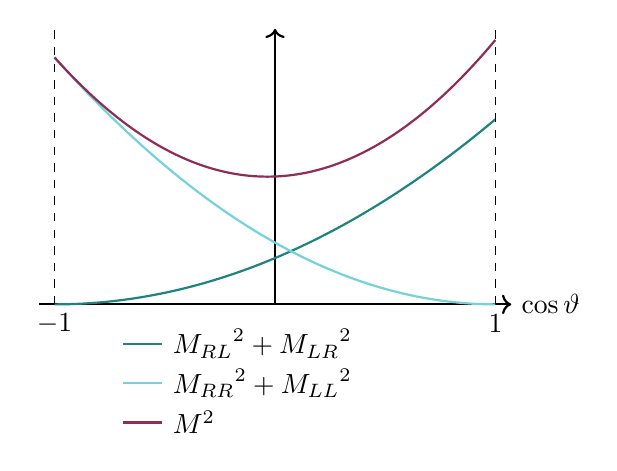
\begin{tikzpicture}
            \draw[thick, ->] (-3, 0) -- (3, 0) node [right] {\(\cos\vartheta\)};
            \draw[thick, ->] (0, 0) -- (0, 3.5);
            \draw[thick, Teal, domain=-2.8:2.8, samples=300] plot (\x, {0.3*(2.8 + \x)^2 / 4});
            \draw[thick, Blue, domain=-2.8:2.8, samples=300] plot (\x, {0.4*(2.8 - \x)^2 / 4});
            \draw[thick, highlight, domain=-2.8:2.8, samples=300] plot (\x, {0.3*(2.8 + \x)^2 / 2.8 + 0.4*(2.8 - \x)^2 / 4});
            \draw[dashed] (2.8, 0) node [below] {1} -- (2.8, 3.5);
            \draw[dashed] (-2.8, 0) node [below] {\(\mathllap{-}1\)} -- (-2.8, 3.5);
            \draw[thick, Teal, text=black] (-1.93, -0.5) -- ++ (0.5, 0) node [right] {\(\abs{\amplitude_{\Right\Left}}^2 + \abs{\amplitude_{\Left\Right}}^2\)};
            \draw[thick, Blue, text=black] (-1.93, -1) -- ++ (0.5, 0) node [right] {\(\abs{\amplitude_{\Right\Right}}^2 + \abs{\amplitude_{\Left\Left}}^2\)};
            \draw[thick, highlight, text=black] (-1.93, -1.5) -- ++ (0.5, 0) node [right] {\(\abs{\amplitude}^2\)};
        \end{tikzpicture}
        \caption[\PZ{} boson decay amplitude]{The \PZ{} boson decay amplitude as a function of \(\cos\vartheta\) where \(\vartheta\) is the scattering angle. Notice that it is not symmetric since the left and right couplings are not the same.}
        \label{fig:Z boson decay amplitude}
    \end{figure}
    
    So far we have been using the propagator term for bosons with denominator \(q^2 - m_{\PZ}^2\),
    This doesn't account for the instability of the \PZ{} boson.
    To correct for this we substitute \(m \mapsto m - i\Gamma_{\PZ}/2\).
    The justification for this is that the time dependence of the wave function is given by \(\psi \propto \e^{-imt}\), and so after this substitution the time dependence of the wave function is \(\psi \propto \e^{-imt}\e^{\Gamma_{\PZ}t/2}\).
    We then have \(\abs{\psi}^2 \propto \e^{-\Gamma_{\PZ}t}\), so the probability of measuring the \PZ{} boson decays exponentially with time.
    
    The propagator denominator is then
    \begin{equation}
        m_{\PZ}^2 \mapsto (m_{\PZ} - i\Gamma_{\PZ}/2)^2 = m_{\PZ}^2 - im_{\PZ}\Gamma_{\PZ} - \frac{1}{4}\Gamma_{\PZ}^2 \approx m_{\PZ}^2 - im_{\PZ}\Gamma_{\PZ}.
    \end{equation}
    Dropping the \(\Gamma_{\PZ}^2\) term is justified as \(\Gamma_{\PZ} = \qty{2.5}{\giga\electronvolt}\) whereas \(m_{\PZ} = \qty{91}{\giga\electronvolt}\).
    This gives the \defineindex{Breit--Wigner propagator} proportional to
    \begin{equation}
        \frac{1}{(s - m_{\PZ}^2)^2 + m_{\PZ}^2\Gamma_{\PZ}^2}.
    \end{equation}
    
    The result is that
    \begin{equation}
        \abs{\amplitude}^2 \propto \abs*{\frac{1}{s - m_{\PZ}^2 + im_{\PZ}\Gamma_{\PZ}}}^2 = \frac{1}{(s - m_{\PZ})^2 + m_{\PZ}^2\Gamma_{\PZ}^2}.
    \end{equation}
    
    A full calculation of the cross section for \(\Pe\APe \to \PZ \to \Pmu\APmu\) gives
    \begin{equation*}
        \sigma(\Pe\APe \to \PZ \to \Pmu\APmu) = \frac{1}{192\pi} \frac{g_{\PZ}^2 s}{(s - m_{\PZ}^2)^2 + m_{\PZ}\Gamma_{\PZ}^2} [(c_{\symup{V}}^{\Penominus})^2 + (c_{\symup{A}}^{\Penominus})^2] [(c_{\symup{V}}^{\upmu})^2 + (c_{\symup{A}}^{\upmu})^2].
    \end{equation*}
    We can simply this by considering the partial widths
    \begin{align}
        \Gamma(\PZ \to \Pe\APe) &= \frac{g_{\PZ}^2 m_{\PZ}}{48\pi} [(c_{\symup{V}}^{\Penominus})^2 + (c_{\symup{A}}^{\Penominus})^2],\\
        \Gamma(\PZ \to \Pmu\APmu) &= \frac{g_{\PZ}^2m_{\PZ}}{48\pi} [(c_{\symup{V}}^{\upmu})^2 + (c_{\symup{A}}^{\upmu})^2]
    \end{align}
    and then we get
    \begin{equation}
        \sigma = \frac{12\pi}{m_{\PZ}^2} \frac{s}{(s - m_{\PZ}^2)^2 + m_{\PZ}^2 \Gamma_{\PZ}^2} \Gamma(\PZ \to \Pe\APe) \Gamma(\PZ \to \Pmu\APmu).
    \end{equation}
    This same result holds for any final state fermion instead of muons.
    
    The cross section of the \PZ{} boson production as a function of the collision energy, \(\sqrt{s}\), is called the \define{\PZ{} boson line shape}\index{Z boson line shape@\PZ{} boson line shape}.
    It can be measured in experiments.
    However, we have to account for second order processes, involving the initial electrons which change the energy of the \PZ{} boson, such as the electron or positron emitting a photon before annihilating into a \PZ{} boson.
    We call accounting for these effects \enquote{unfolding} the data to get just the data we care about for the \PZ{} boson.
    We can use the width of this unfolded data to find the decay rate of the \PZ{} boson and the maximum of the plot should give the mass of the \PZ{} boson as well.
    
    \chapter{Higgs}
    \section{Lagrangians in Quantum Field Theory}
    \subsection{Lagrangians in Classical Mechanics}
    \begin{rmk}
        See \course{Lagrangian Dynamics} for details.
    \end{rmk}
    Consider a system of particles described by coordinates \(q_i\).
    If the kinetic energy is \(T\) and the potential energy is \(V\) then we can define the \defineindex{Lagrangian}
    \begin{equation}
        \lagrangian = T - V,
    \end{equation}
    which is typically a function of the coordinates, \(q_i\), and their time derivatives, \(\dot{q}_i\).
    The equations of motion for the system can be found from the \defineindex{Euler--Lagrange equations}
    \begin{equation}
        \diff{}{t}\left( \diffp{\lagrangian}{\dot{q}_i} \right) = \diffp{\lagrangian}{q_i}.
    \end{equation}
    
    \subsection{Lagrangians in Quantum Field Theory}
    \begin{rmk}
        See \course{Classical Electrodynamics} for Lagrangians in classical field theories and \course{Quantum Field Theory} for Lagrangians in quantum field theories.
    \end{rmk}
    
    If a system can be described by the fields \(\varphi_i\) then the equations of motion for the system can be found by defining the \defineindex{Lagrangian density} (henceforth referred to as the Lagrangian) \(\lagrangianDensity\), which is a function of the fields, \(\varphi_i\), and derivatives of the fields, \(\partial_\mu \varphi_i\), and using the Euler--Lagrange equations for a Lagrangian density:
    \begin{equation}
        \partial_\mu \left( \diffp{\lagrangianDensity}{(\partial_\mu \varphi_i)} \right) = \diffp{\lagrangianDensity}{\varphi_i}.
    \end{equation}
    
    \subsection{Examples}
    A scalar field, \(\varphi\), corresponding to a spin 0 boson of mass \(m\) has the Lagrangian
    \begin{equation}
        \lagrangianDensity = \frac{1}{2}(\partial_\mu \varphi)(\partial^\mu \varphi) - \frac{1}{2}m^2 \varphi^2.
    \end{equation}
    The Euler--Lagrange equations give the Klein--Gordon equation as the equation of motion.
    
    A spinor field, \(\psi\), corresponding to a spin \(1/2\) boson of mass \(m\) has the Lagrangian
    \begin{equation}
        \lagrangianDensity = \diracadjoint{\psi}(i\slashed{\partial} - m)\psi.
    \end{equation}
    The Euler--Lagrange equations give the Dirac equation as the equation of motion.
    Note that we treat \(\psi\) and \(\diracadjoint{\psi}\) as independent fields.
    
    A vector field, \(A_\mu\), corresponding to a spin 1 boson of mass \(m\) has the Lagrangian
    \begin{equation}
        \lagrangianDensity = -\frac{1}{4}F^{\mu\nu}F_{\mu\nu} + \frac{1}{2}m^2 A^\mu A_\mu
    \end{equation}
    where
    \begin{equation}
        F^{\mu\nu} \coloneqq \partial^\mu A^\nu - \partial^\nu A^\mu.
    \end{equation}
    The Euler--Lagrange equations give one Klein--Gordon equation for each component of \(A_\mu\).
    
    In general Lagrangians typically have a kinetic term, with derivatives of the field, a mass term, proportional to the square of the field with constant of proportionality \(m^2/2\), and interaction terms, which are any terms of order more than 2 in the field.
    
    \subsection{Symmetries of the Lagrangian}
    Gauge symmetries are encoded in the Lagrangian by being such as to leave the Lagrangian invariant\footnote{or at least, they leave the action, \(S = \int \lagrangianDensity \dd{^4x}\), invariant, meaning they change the Lagrangian by at most a total derivative term, \(\partial_\mu K\).}
    
    To do this we replace the derivatives with the relevant covariant derivative such that when the fields change according to
    \begin{equation}
        \psi \mapsto \e^{i g \alpha^a T_a} \psi
    \end{equation}
    the Lagrangian is unchanged.
    This is the case if we use the gauge derivative 
    \begin{equation}
        D_\mu = \partial_\mu + igA_\mu
    \end{equation}
    where \(A_\mu\) is some field transforming in such a way as to cancel the extra term that arises from the derivative of the phase factor.
    
    For QED the transformation of interest is the \(\unitary(1)\) transformation
    \begin{equation}
        \psi \mapsto \e^{iq\chi}\psi
    \end{equation}
    and the covariant derivative is
    \begin{equation}
        D_\mu = \partial_\mu + iqA_\mu.
    \end{equation}
    For QCD the transformation of interest is the \(\specialUnitary(3)\) transformation
    \begin{equation}
        \psi \mapsto \e^{i\strongCoupling \alpha^a\lambda_a} \psi
    \end{equation}
    and the covariant derivative is
    \begin{equation}
        D_\mu = \partial_\mu + i\strongCoupling \frac{1}{2} \lambda_a G^a_\mu.
    \end{equation}
    
    For charged current weak interactions the transformation of interest is the \(\specialUnitary(2)\) transformation
    \begin{equation}
        \psi \mapsto \e^{ig_{\PW} \alpha_i\sigma^i/2}\psi
    \end{equation}
    and the covariant derivative is
    \begin{equation}
        D_\mu = \partial_\mu + ig_{\PW} \frac{1}{2}\sigma_i W^i_{\mu}.
    \end{equation}
    
    \section{The Problem with Mass}
    Consider a slight variation of QED where the photon is massive, with mass \(m_{\Pphoton}\), and the electron has mass \(m_{\Penominus}\).
    This theory can be described by the Lagrangian
    \begin{equation}
        \lagrangianDensity = \diracadjoint{\psi} (i\slashed{\partial} - m_{\Penominus})\psi e\diracadjoint{\psi}\slashed{A}\psi - \frac{1}{4} F_{\mu\nu}F^{\mu\nu} + \frac{1}{2}m_{\Pphoton}^2 A_\mu A^\mu.
    \end{equation}
    The problem is that under a \(\unitary(1)\) transformation this extra mass term for the photon breaks the symmetry:
    \begin{equation}
        \frac{1}{2}m_{\Pphoton}^2 A_\mu A^\mu \mapsto \frac{1}{2}m_{\Pphoton}^2(A_\mu - \partial_\mu \chi)(A^\mu - \partial^\mu \chi) \ne \frac{1}{2}m_{\Pphoton}^2 A_\mu A^\mu.
    \end{equation}
    
    So, if we want a \(\unitary(1)\) symmetry then the photon cannot be massive.
    Of course, the photon isn't massive, so this is fine.
    The problem is that \(\specialUnitary(2)\) and \(\specialUnitary(3)\) gauge symmetries similarly prevent the gluons, \PZ, and \PW{} bosons from having mass, and we know that the \PZ{} and \PW{} bosons have mass.
    
    Even more problematic is that as we have set things up so far it is not possible for fermions to have mass either.
    For example, an electron mass term would have the form
    \begin{equation}
        -m_{\Penominus}\diracadjoint{\Penominus}\Penominus = -m_{\Penominus}\diracadjoint{\Penominus} \left[ \frac{1}{2} (1 - \gamma^5) + \frac{1}{2} (1 + \gamma^5) \right]	 \Penominus = -m_{\Penominus} (\diracadjoint{\Penominus}_{\Right}\Penominus_{\Left} + \diracadjoint{\Penominus}_{\Left}\Penominus_{\Right}),
    \end{equation}
    which is not Lorentz invariant, but we require the Lagrangian to be Lorentz invariant in order to get Lorentz invariant results.
    
    \section{The Brout--Englert--Higgs Mechanism}
    The solution to the above problem is to introduce a complex scalar field, \(\varphi\), satisfying the Lagrangian
    \begin{equation}
        \lagrangianDensity = (\partial_\mu\varphi)^\hermit (\partial^\mu \varphi) - V(\varphi)
    \end{equation}
    with potential
    \begin{equation}
        V(\varphi) = \mu^2 \varphi^\hermit \varphi + \lambda(\varphi^\hermit \varphi)^2
    \end{equation}
    where \(\mu^2 < 0\) and \(\lambda > 0\).
    This potential is plotted in \cref{fig:sombrero potential}.
    
    \begin{figure}
        \tikzsetnextfilename{sombrero-potential}
        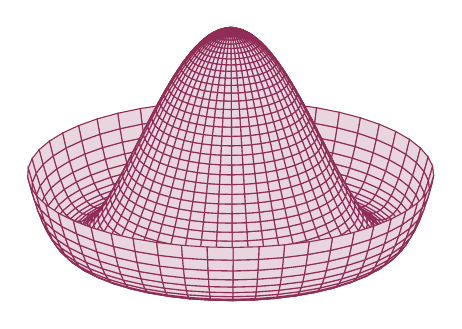
\begin{tikzpicture}
            \begin{axis}[
                hide axis,
                samples=50,
                domain=0:360,
                y domain=0:1.25
                ]
                \addplot3 [surf, shader=flat, draw=highlight, fill=highlight!20, z buffer=sort] ({sin(x)*y}, {cos(x)*y}, {(y^2-1)^2});
            \end{axis}
        \end{tikzpicture}
        \caption{The \enquote{sombrero potential}, \(V(\varphi) = \mu^2\varphi^\hermit\varphi + \lambda(\varphi^\hermit\varphi)^2\) for \(\mu^2 < 0\) and \(\lambda > 0\).}
        \label{fig:sombrero potential}
    \end{figure}
    
    This potential is minimised when \(\varphi = \varphi_0\) with \(\abs{\varphi_0} = \sqrt{-\mu^2/(2\lambda)}\) and \(\arg \varphi \in [0, 2\pi)\).
    This gives a circle of minima.
    We define \(v\), the \defineindex{vacuum expectation value} to be \(v = \sqrt{-\mu^2/\lambda}\), and so the potential is minimised when \(\abs{\varphi_0} = v/\sqrt{2}\).
    
    The \defineindex{Higgs field}, \(\varphi\), is a weak isospin doublet,
    \begin{equation}
        \varphi = 
        \begin{pmatrix}
            \varphi^+\\ \varphi^0
        \end{pmatrix}
        = \frac{1}{\sqrt{2}}
        \begin{pmatrix}
            \varphi_1 + i\varphi_2\\ \varphi_3 + i\varphi_4
        \end{pmatrix}
        .
    \end{equation}
    As with all weak isospin doublets this means that the total weak isospin is \(I = 1/2\).
    Both components also have weak hypercharge \(Y = 1\).
    The top element, \(\varphi^+\), has charge \(Q = +1\) and weak isospin \(I_{\PW}^{(3)} = 1/2\), whereas the bottom element, \(\varphi^0\), has charge \(Q = 0\) and weak isospin \(I_{\PW}^{(3)} = -1/2\).
    
    The minimum, \(\varphi\), must be such that
    \begin{equation}
        \varphi^\hermit \varphi = -\frac{\mu^2}{2\lambda} = \frac{1}{2}v,
    \end{equation}
    or in terms of the real components \(\varphi_i\):
    \begin{equation}
        \varphi^\hermit \varphi = \frac{1}{2}(\varphi_1^2 + \varphi_2^2 + \varphi_3^2 + \varphi_4^2) = \frac{1}{2}v^2.
    \end{equation}
    With this as the only requirement placed on \(\varphi\) we can can assume that the field is in its ground state and only experiences small perturbations away from this state.
    We are also free to choose any particular vacuum state, and so we choose
    \begin{equation}
        \varphi_0 = \frac{1}{\sqrt{2}}
        \begin{pmatrix}
            0\\ v
        \end{pmatrix}
        ,
    \end{equation}
    so \(\varphi^\hermit \varphi = v^2/2\) as required.
    We can then construct a new field, \(h\), such that \(\varphi\) is perturbed by \(h\):
    \begin{equation}
        \varphi(x) = \frac{1}{\sqrt{2}} 
        \begin{pmatrix}
            0\\ v + h(x)
        \end{pmatrix}
        .
    \end{equation}
    
    We then have
    \begin{equation}
        \varphi^\hermit \varphi = \frac{1}{2}(v + h)^2
    \end{equation}
    which we can substitute into \(V(\varphi)\) to get
    \begin{equation}
        V(\varphi) = \mu^2 \frac{1}{2}(v + h)^2 + \lambda\frac{1}{4}(v + h)^4 = -\frac{1}{4}\lambda v^4 + \lambda v^2 h^2 + \lambda v h^3 + \frac{1}{4}\lambda h^4.
    \end{equation}
    Here we've used \(\mu^2 = -\lambda v^2\), which follows from the definition of \(v\).
    
    The Lagrangian is then
    \begin{equation}
        \lagrangianDensity = (\partial_\mu h)^\hermit (\partial^\mu h) + \frac{1}{4}\lambda v^4 - \lambda v^2 h^2 - \lambda v h^3 - \frac{1}{4}\lambda h^4.
    \end{equation}
    We can then interpret this as the Lagrangian for a real scalar field, \(h\), corresponding to a neutral scalar particle, the \defineindex{Higgs boson}, \(\Phiggs\).
    With some practice\footnote{for example, take the \course{Quantum Field Theory} course} it is possible to read off exactly what terms in the Lagrangian correspond to in terms of the particles.
    In this case the terms have the following meaning:
    \begin{description}
        \item[\((\partial_\mu h)^\hermit (\partial^\mu h)\)] This is the kinetic term.
        \item[\(\lambda v^4/4\)] This is a constant, and therefore doesn't effect the physics and can be dropped from the Lagrangian, much like we can always redefine a potential to decide where zero is.
        \item[\(-\lambda v^2 h^2\)] This term is quadratic in the field, and so is a mass term.
        In particular the Higgs boson has mass \(m = \sqrt{2\lambda} v\), which follows by comparison with the expected form of the mass term \(-m^2 h^2/2\).
        \item[\(-\lambda v h^3\)] This is an interaction term corresponding to a vertex with three Higgs bosons.
        The coupling constant is \(\lambda v\), and since this is a scalar field this means that the entire vertex term is simply \(\lambda v\).
        \item[\(-\lambda h^4/4\)] This is an interaction term corresponding to a vertex with four Higgs bosons.
        The coupling constant is \(\lambda/4\), and since this is a scalar field this means that the entire vertex term is simply \(\lambda/4\).
    \end{description}
    
    To summarise, the Higgs boson is a spin zero particle with mass \(m = \sqrt{2\lambda}v\) which can interact with itself in two different ways:
    \begin{equation}
        \tikzsetnextfilename{fd-higgs-interactions}
        \begin{tikzpicture}[
            scalar/.style={dash pattern=on 2pt off 1pt},
            baseline = {(0, 0)}
            ]
            \draw[scalar] (0, 0) -- (-30:0.75);
            \draw[scalar] (0, 0) -- (210:0.75);
            \draw[scalar] (0, 0) -- (90:0.75);
            \node [below] at (0, 0) {\scriptsize \(\lambda v\)};
            \draw[scalar] (2, 0) -- ++ (45:0.75);
            \draw[scalar] (2, 0) -- ++ (135:0.75);
            \draw[scalar] (2, 0) -- ++ (225:0.75);
            \draw[scalar] (2, 0) -- ++ (315:0.75);
            \node [right] at (2.1, 0) {\scriptsize \(\tfrac{1}{4}\lambda\)};
        \end{tikzpicture}
    \end{equation}
    
    \subsection{\texorpdfstring{\PW}{W} and \texorpdfstring{\PZ}{Z} Boson Mass}
    For the electroweak interaction the covariant derivative is
    \begin{equation}
        D_\mu = \partial_\mu + ig_{\PW} \frac{1}{2}\sigma_i W_\mu^i + ig' \frac{Y}{2}B_\mu.
    \end{equation}
    We can replace the derivative in the Higgs Lagrangian with this giving
    \begin{equation}
        \lagrangianDensity = (D_\mu \varphi)^\hermit (D^\mu \varphi)^\hermit - V(\varphi).
    \end{equation}
    Doing so two of the terms we get are
    \begin{gather}
        \frac{1}{8} v^2 g_{\PW}^2 (W_\mu^1 W^{1\mu} + W_\mu^2 W^{2\mu}),\\
        \frac{1}{8}v^2(g_{\PW}W_\mu^3 - g'B_\mu)(g_{\PW} W^{3\mu} - g' B^\mu).
    \end{gather}
    
    Consider the first of these terms.
    We can interpret this as two mass terms, one for \(\PW^1\) bosons and one for \(\PW^2\) bosons.
    Comparing to the expected mass term,
    \begin{equation}
        \frac{1}{2} m_{\PW^{1,2}} W^{1,2}_\mu W^{1,2 \, \mu}
    \end{equation}
    we can see that the \(\PW^{1,2}\) bosons have mass
    \begin{equation}
        m_{\PW^{1,2}} = \frac{1}{2}vg_{\PW}.
    \end{equation}
    Since the \(\PWpm\) boson are given by \(\PWpm = \PW^{1} \pm i\PW^{2}\), so an equal weighting of two equal mass states, the \(\PWpm\) bosons must also have mass
    \begin{equation}
        m_{\PW} = \frac{1}{2}vg_{\PW}.
    \end{equation}
    Since \(m_{\PW}\) and \(g_{\PW}\) can be measured through various weak processes this gives us a way to compute \(v\).
    Putting in known values we get \(v = \qty{246}{\giga\electronvolt}\).
    
    The second term can be interpreted as a mass term also, but with slightly more work.
    We can rewrite this term as
    \begin{align}
        \frac{1}{8} v^2(g_{\PW}W^3_\mu - g'B_\mu) &(g_{\PW}W^{3\mu} - g'B^\mu)\\
        &= \frac{1}{8} v^2
        \begin{pmatrix}
            W^3_{\mu} & B_\mu
        \end{pmatrix}
        \begin{pmatrix}
            g_{\PW}^2 & -g_{\PW}g'\\
            -g_{\PW}g' & g'^2
        \end{pmatrix}
        \begin{pmatrix}
            W^{3\mu}\\ B^\mu
        \end{pmatrix}
        \\
        &= \frac{1}{8}v^2
        \begin{pmatrix}
            A_\mu & Z_\mu
        \end{pmatrix}
        \begin{pmatrix}
            0 & 0\\
            0 & g_{\PW}^2 + g'^2
        \end{pmatrix}
        \begin{pmatrix}
           A^\mu\\ Z^\mu
        \end{pmatrix}
        \\
        &= \frac{1}{8}v^2 (g_{\PW}^2 + g'^2) Z_\mu Z^\mu.
    \end{align}
    Here we've made a change of basis from \(W^3\) and \(B\) to \(A\) and \(Z\), which are by construction an orthonormal basis, as well as corresponding to physical particles.
    We can identify this as two mass terms, the obvious one being
    \begin{equation}
        \frac{1}{2}m_{\PZ}^2 = \frac{1}{8} v^2 (g_{\PW}^2 + g'^2) \implies m_{\PZ} = \frac{1}{2}v\sqrt{g_{\PW}^2 + g'^2},
    \end{equation}
    and the second less obvious being
    \begin{equation}
        \frac{1}{2}m_{\Pphoton}^2 = 0 \implies m_{\Pphoton} = 0.
    \end{equation}
    So we get the \PZ{} boson mass and as expected the photon is massless.
    
    Recall the definition of \(A_\mu\) and \(Z_\mu\):
    \begin{align}
        A_\mu &= +B_\mu \cos\vartheta_{\PW} + W_\mu^3\sin\vartheta_{\PW},\\
        Z_\mu &= -B_\mu \sin\vartheta_{\PW} + W_\mu^3\cos\vartheta_{\PW}.
    \end{align}
    Using the matrix above we also see that
    \begin{align}
        A_\mu &= \frac{1}{\sqrt{g_{\PW}^2 + g'^2}} (g_{\PW} B_\mu + g'W_\mu^3),\\
        Z_\mu &= \frac{1}{\sqrt{g_{\PW}^2 + g'^2}} (-g'B_\mu + g_{\PW}W_\mu^3).
    \end{align}
    Hence, we can identify
    \begin{equation}
        \cos\vartheta_{\PW} = \frac{g_{\PW}}{\sqrt{g_{\PW}^2 + g'^2}}, \qqand \sin\vartheta_{\PW} = \frac{g'}{\sqrt{g_{\PW}^2 + g'^2}}.
    \end{equation}
    
    Extra terms in the Lagrangian which we haven't accounted for here give interactions between the Higgs boson and the \PW{} or \PZ{} bosons:
    \begin{equation}
        \tikzsetnextfilename{fd-higgs-WZ-interactions}
        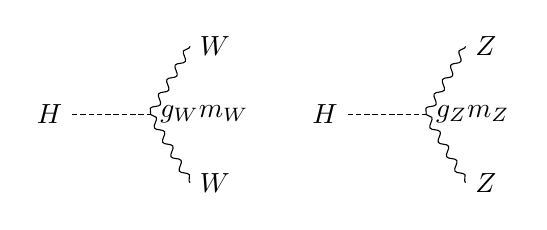
\begin{tikzpicture}[
            photon/.style={decoration={snake, amplitude=1.25, segment length=6}, decorate},
            scalar/.style={dash pattern=on 2pt off 1pt},
            baseline = {(0, 0)}
            ]
            \draw[scalar] (-1, 0) node [left] {\Phiggs} -- (0, 0);
            \draw[photon] (0, 0) -- (60:1) node [right] {\PW};
            \draw[photon] (0, 0) -- (-60:1) node [right] {\PW};
            \node [right] at (0, 0) {\(g_{\PW} m_{\PW}\)};
            \begin{scope}[xshift=3.5cm]
                \draw[scalar] (-1, 0) node [left] {\Phiggs} -- (0, 0);
                \draw[photon] (0, 0) -- (60:1) node [right] {\PZ};
                \draw[photon] (0, 0) -- (-60:1) node [right] {\PZ};
                \node [right] at (0, 0) {\(g_{\PZ} m_{\PZ}\)};
            \end{scope}
        \end{tikzpicture}
    \end{equation}
    
    \subsection{Fermion Mass}
    It is possible for the Higgs field to interact with massive fermions.
    We can do this by introducing an interaction term.
    For an electron this term might take the form
    \begin{equation}
        \lagrangianDensity_{\Penominus} = -\frac{g_{\Penominus}}{\sqrt{2}} v(\diracadjoint{\Penominus}_{\Left}e_{\Right} + \diracadjoint{\Penominus}_{\Right}\Penominus_{\Left}) - \frac{g_{\Penominus}}{\sqrt{2}} h(\diracadjoint{\Penominus}_{\Left}e_{\Right} + \diracadjoint{\Penominus}_{\Right}\Penominus_{\Left})
    \end{equation}
    for some coupling, \(g_{\Penominus}\) between the Higgs boson and the electron.
    This can be Lorentz invariant as we now have an extra field, \(h\), which transforms in just the right way to undo the changes of a Lorentz transformation.
    
    If we take \(g_{\Penominus} = m_{\Penominus}\sqrt{2}/v\) then this term becomes
    \begin{align}
        \lagrangianDensity_{\Penominus} &= -m_{\Penominus} (\diracadjoint{\Penominus}_{\Left}e_{\Right} + \diracadjoint{\Penominus}_{\Right}\Penominus_{\Left}) - \frac{m_{\Penominus}}{v} h(\diracadjoint{\Penominus}_{\Left}e_{\Right} + \diracadjoint{\Penominus}_{\Right}\Penominus_{\Left})\\
        &= m_{\Pe}(\diracadjoint{\Penominus}\Penominus) - \frac{m_{\Pe}}{v}(\diracadjoint{\Penominus}\Penominus).
    \end{align}
    We can interpret this as a mass term for the electron as well as an interaction between two electrons and the Higgs with vertex term \(m_{\Penominus}/v\):
    \begin{equation}
        \tikzsetnextfilename{fd-higgs-electron-interactions}
        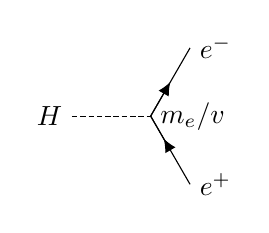
\begin{tikzpicture}[
            >={Latex[width=1.5mm]},
            scalar/.style={dash pattern=on 2pt off 1pt},
            baseline = {(0, 0)}
            ]
            \draw[scalar] (-1, 0) node [left] {\Phiggs} -- (0, 0);
            \draw (0, 0) -- (60:1) node [right] {\Pe};
            \draw (0, 0) -- (-60:1) node [right] {\APe};
            \draw[->] (0, 0) -- (60:0.5);
            \draw[-<] (0, 0) -- (-60:0.5);
            \node [right] at (0, 0) {\(m_{\Penominus}/v\)};
        \end{tikzpicture}
    \end{equation}
    
    Exactly the same logic applies to any of the other massive fermions.
    The coupling to the Higgs boson is proportional to the mass of the fermion.
    
    \section{Higgs Boson Decay}
    The Higgs boson has mass \(m_{\Phiggs} = \qty{125.4(4)}{\giga\electronvolt}\).
    Since it couples to any massive fermion it can decay into any massive fermion except the top quark, since the top quark is too massive for this decay to occur.
    The heavier the fermion is the more likely it as the result of a Higgs decay.
    
    The \PZ{} and \PW{} bosons are also too massive for the Higgs to decay into them.
    However, the Higgs can decay into a real \PW{} or \PZ{} and a virtual \PW{} or \PZ{} boson, which we denote \(\PW^*\) or \(\PZ^*\).
    Since the coupling is also proportional to mass for the \PW{} and \PZ{} bosons these decays are quite common.
    
    In addition to these direct decays the Higgs can also decay into massless particles via an intermediary virtual particle triangle, such as
    \begin{equation}
        \tikzsetnextfilename{fd-higgs-decay-to-massless}
        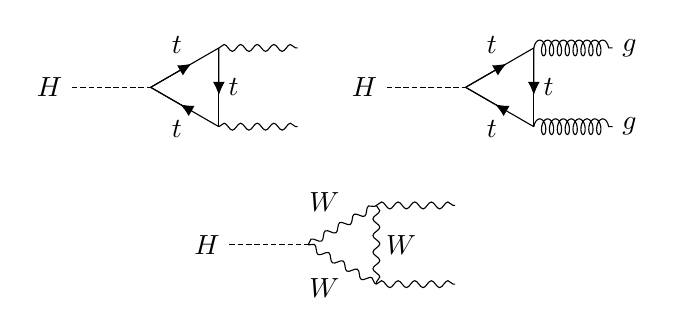
\begin{tikzpicture}[
            >={Latex[width=1.5mm]},
            photon/.style={decoration={snake, amplitude=1.25, segment length=6}, decorate},
            scalar/.style={dash pattern=on 2pt off 1pt},
            gluon/.style={decoration={coil, amplitude=1mm, segment length=1mm}, decorate},
            baseline = {(0, 0)}
            ]
            \draw[scalar] (-1, 0) node [left] {\Phiggs} -- (0, 0);
            \draw (0, 0) -- (30:1);
            \draw (0, 0) -- (-30:1);
            \draw (30:1) -- (-30:1);
            \draw[->] (0, 0) -- (30:0.6) node [above left] {\Pt};
            \draw[-<] (0, 0) -- (-30:0.6) node [below left] {\Pt};
            \draw[->] (30:1) -- (0.866, -0.1) node [right, yshift=0.1cm] {\Pt};
            \draw[photon] (30:1) -- ++ (1, 0) node [right] {\Pphoton};
            \draw[photon] (-30:1) -- ++ (1, 0) node [right] {\Pphoton};
            
            \begin{scope}[xshift=4cm]
                \draw[scalar] (-1, 0) node [left] {\Phiggs} -- (0, 0);
                \draw (0, 0) -- (30:1);
                \draw (0, 0) -- (-30:1);
                \draw (30:1) -- (-30:1);
                \draw[->] (0, 0) -- (30:0.6) node [above left] {\Pt};
                \draw[-<] (0, 0) -- (-30:0.6) node [below left] {\Pt};
                \draw[->] (30:1) -- (0.866, -0.1) node [right, yshift=0.1cm] {\Pt};
                \draw[gluon] (30:1) -- ++ (1, 0) node [right] {\Pg};
                \draw[gluon] (-30:1) -- ++ (1, 0) node [right] {\Pg};
            \end{scope}
            
            \begin{scope}[xshift=2cm, yshift=-2cm]
                \draw[scalar] (-1, 0) node [left] {\Phiggs} -- (0, 0);
                \draw[photon] (0, 0) -- (30:1);
                \draw[photon] (0, 0) -- (-30:1);
                \draw[photon] (30:1) -- (-30:1);
                \node[above left] at (30:0.6) {\PW};
                \node[below left] at (-30:0.6) {\PW};
                \node[right] at (0.866, 0) {\PW};
                \draw[photon] (30:1) -- ++ (1, 0) node [right] {\Pphoton};
                \draw[photon] (-30:1) -- ++ (1, 0) node [right] {\Pphoton};
            \end{scope}
        \end{tikzpicture}
    \end{equation}
    
    Consider the decay
    \tikzsetnextfilename{fd-higgs-bottom-decay}
    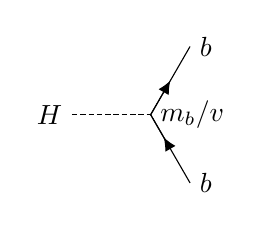
\begin{tikzpicture}[
        >={Latex[width=1.5mm]},
        scalar/.style={dash pattern=on 2pt off 1pt},
        baseline = {(0, 0)}
        ]
        \draw[scalar] (-1, 0) node [left] {\Phiggs} -- (0, 0);
        \draw (0, 0) -- (60:1) node [right] {\Pb};
        \draw (0, 0) -- (-60:1) node [right] {\APb};
        \draw[->] (0, 0) -- (60:0.5);
        \draw[-<] (0, 0) -- (-60:0.5);
        \node [right] at (0, 0) {\(m_{\Pb}/v\)};
    \end{tikzpicture}
    We pick bottom quarks as the most likely decay product since they are the most massive fermions to which a Higgs boson can decay.
    The amplitude for this decay is
    \begin{equation}
        \amplitude = \frac{m_{\Pb}}{v} \diracadjoint{u}(p_2) v(p_3)
    \end{equation}
    where \(p_2\) is the momentum of the \(\Pb\) quark and \(p_3\) the momentum of the \(\APb\) antiquark.
    If we account for the helicities of the quarks there are two nonzero amplitudes:
    \begin{equation}
        \amplitude_{\uparrow\uparrow} = -\amplitude_{\downarrow\downarrow} = \frac{m_{\Pb}}{v}2E.
    \end{equation}
    Both fermions must have the same helicity as the Higgs boson is spin 0 and the momenta of the fermions are equal and opposite, and their spins must be anti-aligned to conserve angular momentum, meaning either both have their momentum and spin aligned, or both have their momentum and spin anti-aligned.
    
    The total amplitude squared for decay to bottom quarks (at tree level) is thus
    \begin{equation}
        \amplitude^2 = \abs{\amplitude_{\uparrow\uparrow}}^2 + \abs{\amplitude_{\downarrow\downarrow}}^2 = \frac{2m_{\Pb}^2m_{\Phiggs}^2}{v^2}
    \end{equation}
    having used \(2E = m_{\Phiggs}\) as the energy of each fermion.
    The total decay rate for this particular decay channel is
    \begin{equation}
        \Gamma(\Phiggs \to \Pb \APb) = \numberofcolors \frac{m_{\Pb}^2 m_{\Phiggs}}{8\pi v^2}.
    \end{equation}
    So the decay rate is proportional to the mass of the fermion squared, justifying our earlier statement that decay to bottom quarks is more likely.
    
    \section{Higgs Bosons at the LHC}
    \epigraph{Astronomers get pictures of the galaxy. Particle physicists get histograms.}{}
    \Cref{fig:higgs production} shows some processes creating Higgs bosons common at the LHC.
    We've also seen common decays, including decays to \PW{}/\PZ{} bosons, with one being virtual, and decays to photons or photons and \PZ{} bosons, via a triangle of massive particles.
    Another useful decay is decay to a muon and antimuon or tau and antitau.
    These are more common than decays to electrons, because the fermions are more massive, but not as common as decay to some of the heavier quarks.
    However, it's easier to detect muons and taus.
    
    \begin{figure}
        \tikzsetnextfilename{fd-higgs-production-LHC}
        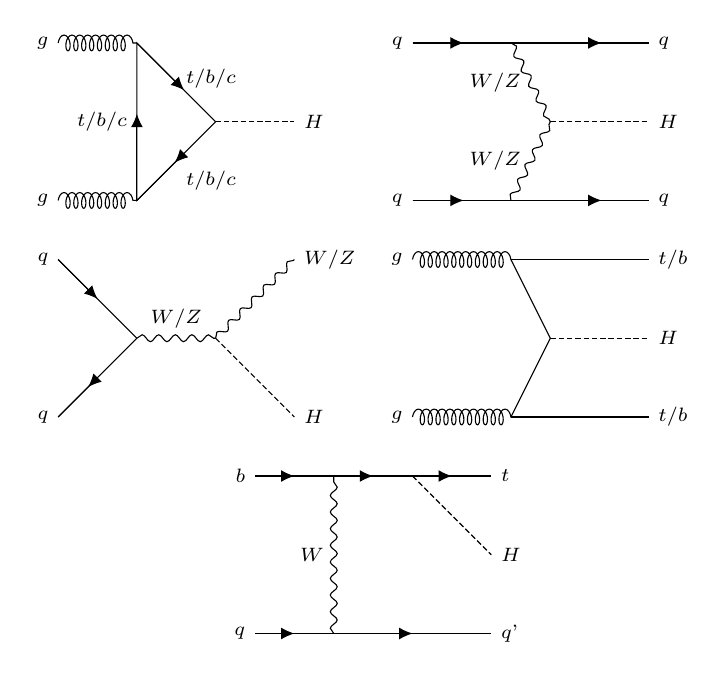
\begin{tikzpicture}[
            >={Latex[width=1.5mm]},
            boson/.style={decoration={snake, amplitude=1.25, segment length=6}, decorate},
            scalar/.style={dash pattern=on 2pt off 1pt},
            gluon/.style={decoration={coil, amplitude=1mm, segment length=1mm}, decorate},
            font=\scriptsize
            ]
            \draw[gluon] (0, 0) node [left] {\Pg} -- (1, 0);
            \draw[gluon] (0, 2) node [left] {\Pg} -- (1, 2);
            \draw (1, 0) -- (1, 2) -- (2, 1) -- cycle;
            \draw[scalar] (2, 1) -- (3, 1) node [right] {\Phiggs};
            \draw[->] (1, 0) -- (1, 1.1) node [left, yshift=-0.1cm] {\Pt/\Pb/\Pc};
            \draw[->] (1, 2) -- (1.6, 1.4) node [above right, xshift=-0.1cm, yshift=-0.1cm] {\Pt/\Pb/\Pc};
            \draw[-<] (1, 0) -- (1.6, 0.6) node [below right, xshift=-0.1cm, yshift=-0.1cm] {\Pt/\Pb/\Pc};
            
            \begin{scope}[xshift=4.5cm]
                \draw (0, 0) node [left] {\Pq} -- (3, 0) node [right] {\Pq};
                \draw[->] (0, 0) -- (0.65, 0);
                \draw[->] (1.75, 0) -- (2.4, 0);
                \draw (0, 2) node [left] {\Pq} -- (3, 2) node [right] {\Pq};
                \draw[->] (0, 2) -- (0.65, 2);
                \draw[->] (1.75, 2) -- (2.4, 2);
                \draw[boson] (1.25, 0) -- (1.75, 1) node [midway, left] {\PW/\PZ};
                \draw[boson] (1.25, 2) -- (1.75, 1) node [midway, left] {\PW/\PZ};
                \draw[scalar] (1.75, 1) -- (3, 1) node [right] {\Phiggs};
            \end{scope}
            
            \begin{scope}[yshift=-2.75cm]
                \draw (0, 0) node [left] {\Pq} -- (1, 1);
                \draw (0, 2) node [left] {\Pq} -- (1, 1);
                \draw[-<] (0, 0) -- (0.5, 0.5);
                \draw[->] (0, 2) -- (0.5, 1.5);
                \draw[boson] (1, 1) -- (2, 1) node [midway, above] {\PW/\PZ};
                \draw[scalar] (2, 1) -- (3, 0) node [right] {\Phiggs};
                \draw[boson] (2, 1) -- (3, 2) node [right] {\PW/\PZ};
            \end{scope}
            
            \begin{scope}[xshift=4.5cm, yshift=-2.75cm]
                \draw[gluon] (0, 0) node [left] {\Pg} -- (1.25, 0);
                \draw[gluon] (0, 2) node [left] {\Pg} -- (1.25, 2);
                \draw (1.25, 0) -- (3, 0) node [right] {\Pt/\Pb};
                \draw (1.25, 2) -- (3, 2) node [right] {\Pt/\Pb};
                \draw (1.25, 0) -- (1.75, 1);
                \draw (1.25, 2) -- (1.75, 1);
                \draw[scalar] (1.75, 1) -- (3, 1) node [right] {\Phiggs};
            \end{scope}
            
            \begin{scope}[yshift=-5.5cm, xshift=2.5cm]
                \draw (0, 0) node [left] {\Pq} -- (3, 0) node [right] {\Pq'};
                \draw (0, 2) node [left] {\Pb} -- (3, 2) node [right] {\Pt};
                \draw[->] (0, 0) -- (0.5, 0);
                \draw[->] (1, 0) -- (2, 0);
                \draw[->] (0, 2) -- (0.5, 2);
                \draw[->] (1, 2) -- (1.5, 2);
                \draw[->] (2, 2) -- (2.5, 2);
                \draw[boson] (1, 0) -- (1, 2) node [midway, left] {\PW};
                \draw[scalar] (2, 2) -- (3, 1) node [right] {\Phiggs};
            \end{scope}
        \end{tikzpicture}
        \caption{Common processes creating Higgs bosons at the LHC.}
        \label{fig:higgs production}
    \end{figure}
    
    \Cref{fig:higgs discovery} shows one of the plots CERN used to announce the discovery of the Higgs boson in 2012.
    A slight peak at \qty{126.5}{\giga\electronvolt} corresponds to a resonance for creating the Higgs boson.
    
    \begin{figure}
        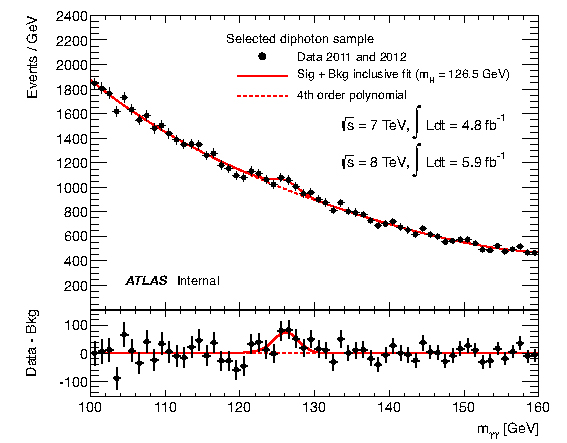
\includegraphics[width=0.8\textwidth]{images/higgs-discovery}
        \caption{One of the plots used when CERN announced the discovery of the Higgs boson. The peak at \qty{126.5}{\giga\electronvolt} is due to the Higgs boson, although later measurements bring the mass down to \qty{125.4}{\giga\electronvolt}. Image taken from \cite{higgsDiscovery}}
        \label{fig:higgs discovery}
    \end{figure}
    
    \part{Non-Examinable}
    \chapter{Neutrinos}
    \begin{rmk}
        The new content appearing in this chapter is non-examinable.
    \end{rmk}
    
    \section{Neutrino Basics}
    Neutrinos are spin \(1/2\), electrically neutral, colour neutral leptons.
    There are three neutrinos appearing in the standard model.
    Neutrinos are massive particles, but there masses are significantly lower than the masses of the other standard model particles.
    The exact masses of the neutrinos isn't known, since they are simply too light to measure.
    The best limits we have on their masses come from cosmological measurements and restrict the sum of their masses to be less than \(\qty{0.12}{\electronvolt}\), less than four millionths the mass of the next lightest standard model particle, the electron.
    
    In addition to being very light neutrinos also have no electric or colour charge, and so interact only through the weak force.
    This means that the cross section for most neutrino scattering processes is very small.
    So neutrinos hardly ever interact.
    
    So far we have only observed left handed helicity neutrinos and right handed helicity antineutrinos.
    Partly this is due to the fact that charged weak current interactions couple neutrinos to the heavier leptons, whereas neutral current interactions couple neutrinos to themselves, so the charged current interactions are easier to observe.
    It is hypothesised that right handed helicity neutrinos do exist, and they are a potential candidate for dark matter.
    These results, only left handed particles and right handed antiparticles, are what one would expect for massless particles, so one solution is that the mechanism giving neutrinos mass somehow preserves this asymmetry.
    
    \section{Number of Neutrinos}
    By considering \PZ{} boson decays into either hadrons, charged leptons, or neutrinos we get
    \begin{equation}
        \Gamma_{\PZ} = N_{\ell}\Gamma_{\ell \ell} + \Gamma_{\text{hadrons}} + N_{\upnu}\Gamma_{\upnu\upnu}.
    \end{equation}
    Here \(\ell\) are the charged leptons, of which there are \(N_{\ell}\) generations, and \(\upnu\) are the neutrinos, of which there are \(N_{\upnu}\) generations.
    The hadrons term covers all hadrons, from quark-antiquark pairs, forming double jets, to more complex multi-jet events.
    Rearranging, using measured values for \(\Gamma_{\ell \ell}\), \(N_{\ell}\), and \(\Gamma_{\text{hadrons}}\), and theoretical values for \(\Gamma_{\upnu\upnu}\) we find that \(N_{\upnu} = 3\), or more precisely,
    \begin{equation}
        N_{\upnu} = \num{2.9840(82)}.
    \end{equation}
    We then conclude that there are only 3 generations of neutrinos, with mass less than \(m_{\PZ}/2\), in the standard model.
    
    \section{Oscillations}
    The \define{weak eigenstates}\index{weak eigenstate} of the neutrino are \Pnue, \Pnumu, and \Pnutau.
    These are also called the flavour eigenstates.
    We can never directly observe neutrinos, instead we detect them via weak interactions.
    These weak eigenstates are defined by which charged lepton they are produced alongside, so by definition
    \begin{itemize}
        \item \Pnue{} is the neutrino state produced along with an electron,
        \item \Pnumu{} is the neutrino state produced along with an muon,
        \item \Pnutau{} is the neutrino state produced along with an tau.
    \end{itemize}
    
    When we are considering propagating neutrinos we instead consider neutrino mass eigenstates.
    For now consider only electron and muon neutrinos.
    We can then define the mass eigenstates \Pnuone{} and \Pnutwo.
    These are the states which propagate, and they do so as plane waves, if the initial state is \(\ket{\Pnuone}\) then at some time \(t\) the state is
    \begin{equation}
        \ket{\Pnuone, t} = \e^{-ip_1 \cdot x}\ket{\Pnuone},
    \end{equation}
    and similar for \Pnutwo.
    The neutrino flavour eigenstates are then orthogonal linear combinations of these mass eigenstates given by
    \begin{equation}
        \begin{pmatrix}
            \Pnue\\ \Pnumu
        \end{pmatrix}
        =
        \begin{pmatrix}
            \cos \vartheta & \sin \vartheta\\
            -\sin \vartheta & \cos \vartheta
        \end{pmatrix}
        \begin{pmatrix}
            \Pnuone\\ \Pnutwo
        \end{pmatrix}
    \end{equation}
    where \(\vartheta\) is some mixing angle to be determined from measurements.
    
    Using this we can decompose a Feynman diagram involving the flavour eigenstates into a sum of Feynman diagrams involving mass eigenstates and modified vertices.
    For example,
    \begin{equation*}
        \tikzsetnextfilename{fd-up-to-down-positron-via-neutrino-mass-and-flavour-states}
        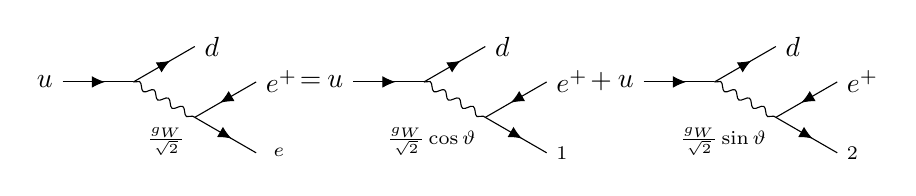
\begin{tikzpicture}[
            boson/.style={decoration={snake, amplitude=1.25, segment length=6}, decorate},
            >={Latex[width=1.5mm]},
            baseline=(current bounding box),
            fermion/.style={decoration={markings, mark=at position #1 with {\arrow{>}}}, postaction=decorate},
            fermion/.default=0.5,
            antifermion/.style={decoration={markings, mark=at position #1 with {\arrow{<}}}, postaction=decorate},
            antifermion/.default=0.5,
            scale=0.9
            ]
            \draw[fermion=0.6] (0, 0) node [left] {\Pu} -- (1, 0);
            \draw[fermion=0.6] (1, 0) -- ++ (30:1) node [right] {\Pd};
            \draw[boson] (1, 0) -- ++ (-30:1) coordinate (A) node [below left] {\(\scriptstyle \frac{g_{\PW}}{\sqrt{2}}\)};
            \draw[antifermion=0.6] (A) -- ++ (30:1) node [right] {\APe};
            \draw[fermion=0.6] (A) -- ++ (-30:1) node [right] {\Pnue};
            
            \begin{scope}[xshift=4.1cm]
                \draw[fermion=0.6] (0, 0) node [left] {\Pu} -- (1, 0);
                \draw[fermion=0.6] (1, 0) -- ++ (30:1) node [right] {\Pd};
                \draw[boson] (1, 0) -- ++ (-30:1) coordinate (A) node [below left] {\(\scriptstyle \frac{g_{\PW}}{\sqrt{2}} \cos \vartheta\)};
                \draw[antifermion=0.6] (A) -- ++ (30:1) node [right] {\APe};
                \draw[fermion=0.6] (A) -- ++ (-30:1) node [right] {\Pnuone};
            \end{scope}
            \begin{scope}[xshift=8.2cm]
                \draw[fermion=0.6] (0, 0) node [left] {\Pu} -- (1, 0);
                \draw[fermion=0.6] (1, 0) -- ++ (30:1) node [right] {\Pd};
                \draw[boson] (1, 0) -- ++ (-30:1) coordinate (A) node [below left] {\(\scriptstyle \frac{g_{\PW}}{\sqrt{2}} \sin \vartheta\)};
                \draw[antifermion=0.6] (A) -- ++ (30:1) node [right] {\APe};
                \draw[fermion=0.6] (A) -- ++ (-30:1) node [right] {\Pnutwo};
            \end{scope}
            
            \node at (3.5, 0) {\(=\)};
            \node at (7.6, 0) {\(+\)};
        \end{tikzpicture}
    \end{equation*}
    
    Now suppose that the neutrino interacts at a detector a distance \(L\) from its initial position and at time \(T\).
    Then the phase of the neutrino mass state is
    \begin{equation}
        \varphi_i = -p_i \cdot x = E_i T - \abs{\vv{p}_i} L.
    \end{equation}
    If the neutrino is produced in a process involving electrons then it will initially be produced in an electron neutrino flavour eigenstate.
    When it interacts it will then be in the state
    \begin{equation}
        \ket{\psi(L, t)} = \cos(\vartheta) \e^{-i\varphi_1} \ket{\Pnuone} + \sin(\vartheta) \e^{-i\varphi_2}\ket{\Pnutwo}.
    \end{equation}
    If the \(\Pnuone\) and \(\Pnutwo\) eigenstates have the same mass then the phase relationship is constant and the weak eigenstates are a coherent linear combination of the mass eigenstates.
    If the mass eigenstates do not have the same mass then the relationship between the phases changes as the neutrino propagates.
    
    Inverting the relationship between the mass and flavour eigenstates we can write this as
    \begin{align}
        \ket{\psi(L, T)} &= \cos(\vartheta)(\cos(\vartheta) \ket{\Pnue} - \sin\vartheta\ket{\Pnumu})\e^{-i\varphi_1} + \sin(\vartheta)(\sin(\vartheta)\ket{\Pnue} + \cos(\vartheta)\ket{\Pnumu})\e^{-i\varphi_2}\\
        &= \e^{-i\varphi_1}[(\cos^2\vartheta + \e^{i\Delta\varphi_{12}}\sin^2\vartheta) \ket{\Pnue} - (1 - \e^{i\Delta\varphi_{12}})\cos(\vartheta)\sin(\vartheta) \ket{\Pnumu}]
    \end{align}
    where
    \begin{equation}
        \Delta \varphi_{12} = \varphi_1 - \varphi_2 = (E_1 - E_2)T - (\abs{\vv{p}_1} - \abs{\vv{p}_2})L.
    \end{equation}
    Writing this as
    \begin{equation}
        \ket{\psi(L, T)} = c_{\Penominus} \ket{\Pnue} + c_{\upmu} \ket{\Pnumu}
    \end{equation}
    with \(c_{\Penominus} = \braket{\Pnue}{\psi}\) and \(c_{\upnu} = \braket{\Pnumu}{\psi}\) we can find the probability that the neutrino will be detected in the muon flavour eigenstate:
    \begin{align}
        P(\Pnue \to \Pnumu) &= c_\mu c_\mu^*\\
        &= (1 - \e^{i\Delta\varphi_{12}})(1 - \e^{-i\Delta\varphi_{12}})\cos^2(\vartheta)\sin^2(\vartheta)\\
        &= \sin^2(2\vartheta)\sin^2\left( \frac{\Delta\varphi_{12}}{2} \right).
    \end{align}
    
    Since both mass eigenstates correspond to the same particle we can assume that the momenta are the same for both, say \(p_1 = p_2 = p\), in which case we have
    \begin{equation}
        \Delta\varphi_{12} = (E_1 - E_2)T = \left[ p \sqrt{1 + \frac{m_1^2}{p^2}} - p \sqrt{1 + \frac{m_2^2}{p^2}} \right] T.
    \end{equation}
    Since \(E \ll m\) we can use the binomial expansion to write
    \begin{equation}
        \sqrt{1 + \frac{m^2}{p^2}} \approx 1 + \frac{m^2}{2p^2},
    \end{equation}
    giving
    \begin{equation}
        \Delta\varphi_{12} \approx \frac{m_1^2 - m_2^2}{2p} L,
    \end{equation}
    where we assume that \(T \approx L\) in natural units, that is that the neutrinos are propagating at almost the speed of light.
    One slight subtlety here is that the assumption of equal momenta for the mass eigenstates means that they are actually travelling at different speeds, and therefore travel different distances in the same time.
    The way around this is to properly consider them as wave packets, rather than localised particles.
    The result we get is the same however.
    
    Combining these results and using \(p \approx E\) we have
    \begin{equation}
        P(\Pnue \to \Pnumu) = \sin^2(2\vartheta) \sin^2\left( \frac{\Delta m_{12}^2 L}{4E} \right)
    \end{equation}
    with \(\Delta m_{12}^2 = m_2^2 - m_1^2\).
    
    The first factor of \(\sin^2(2\vartheta)\) here is a constant, depending on the mixing angle, and experimental results give \(\sin^2(2\vartheta) \approx 0.8\).
    The second controls how the neutrino oscillates between the two flavour eigenstates.
    Experiments give \(\Delta m_{12}^2 = \qty{0.003}{\electronvolt\squared}\).
    The wavelength of the oscillations is \(\lambda_{\text{osc}} = 4\pi E/(\Delta m_{12}^2)\).
    The probability of measuring the neutrino to be in either flavour eigenstate is plotted as a function of \(L\) in \cref{fig:neutrino mixing}.
    
    \begin{figure}
        \def\tempone{\scriptstyle P(\Pnue \to \Pnue)}
        \def\temptwo{\scriptstyle P(\Pnue \to \Pnumu)}
        \tikzsetnextfilename{neutrino-mixing}
        \begin{tikzpicture}
            \begin{axis}[
                domain=0:1000,
                no markers,
                width=0.8\textwidth,
                height=0.6\textwidth,
                samples=100,
                legend entries={\(\tempone\), \(\temptwo\)},
                legend style={
                    at={(0.99, 0.5)},
                    anchor=east,
                    draw=none
                },
                title=Neutrino Mixing During Propagation,
                xlabel=Distance / \unit{\kilo\metre},
                ylabel=Probability
                ]
                \addplot[thick, Burgandy] (x, {0.8*sin(deg(x/275))^2});
                \addplot[thick, Teal] (x, {1 - 0.8*sin(deg(x/275))^2});
            \end{axis}
        \end{tikzpicture}
        \undef\tempone
        \undef\temptwo
        \caption[Neutrino mixing during propagation]{Neutrino mixing during propagation. Notice that the probability of finding the neutrino in the \Pnue{} eigenstate varies between 1 and \(0.2\), whereas the probability of finding the neutrino in the \Pnumu{} eigenstate varies between 0 and \(0.8\).}
        \label{fig:neutrino mixing}
    \end{figure}
    
    In reality we know that there are three neutrino flavours, and three neutrino mass eigenstates.
    These are related by the Pontecorvo--Maki--Nakagawa--Sakata matrix, or the PMNS\glossary[acronym]{PMNS}{Pontecorvo--Maki--Nakagawa--Sakata} matrix for short, \(U\):
    \begin{equation}
        \begin{pmatrix}
            \Pnue\\ \Pnumu\\ \Pnutau
        \end{pmatrix}
        =
        \begin{pmatrix}
            U_{\Penominus 1} & U_{\Penominus 2} & U_{\Penominus 3}\\
            U_{\upmu 1} & U_{\upmu 2} & U_{\upmu 3}\\
            U_{\uptau 1} & U_{\uptau 2} & U_{\uptau 3}
        \end{pmatrix}
        \begin{pmatrix}
            \Pnuone\\ \Pnutwo\\ \Pnuthree
        \end{pmatrix}
        .
    \end{equation}
    Note that to conserve probability this matrix must be unitary.
    
    Typically we factorise the PMNS matrix as
    \begin{equation}
        U = 
        \begin{pmatrix}
            1 & 0 & 0\\
            0 & c_{23} & s_{23}\\
            0 & -s_{23} & c_{23}
        \end{pmatrix}
        \begin{pmatrix}
            c_{13} & 0 & s_{13}\e^{-i\delta}\\
            0 & 1 & 0\\
            -s_{13}\e^{i\delta} & 0 & c_{13}
        \end{pmatrix}
        \begin{pmatrix}
            c_{12} & s_{12} & 0\\
            -s_{12} & c_{12} & 0\\
            0 & 0 & 1
        \end{pmatrix}
        .
    \end{equation}
    Here \(c_{ij} = \cos \vartheta_{ij}\) and \(s_{ij} = \sin \vartheta_{ij}\) with \(\vartheta_{12}\), \(\vartheta_{23}\), and \(\vartheta_{13}\) mixing angles, and \(\delta\) a complex phase.
    We Measurements of solar neutrinos allow us to measure \(\vartheta_{12}\), measurements of atmospheric neutrinos allow us to measure \(\vartheta_{23}\), and measurements in reactors allow us to measure \(\vartheta_{13}\).
    We are yet to measure \(\delta\), but it is hoped that future beam experiments will allow for this value to be measured.
    On top of these parameters we also have two mass differences, \(\Delta m_{21}^2 = m_2^2 - m_1^2\) and \(\Delta m_{23}^2 = m_3^2 - m_2^2\).
    This makes six parameters which are not explained by the theory but have to be measured and input into the standard model to produced predictions.
    
    \section{Neutrino Production}
    Cosmic rays produce neutrinos in the atmosphere.
    These form as parts of showers of particles from the initial cosmic ray scattering off an atmospheric particle.
    In these reactions we find that approximately twice as many muon neutrinos and antineutrinos are produced as electron neutrinos and antineutrinos.
    
    We can detect these with neutrino detectors.
    The typical design for these is to dig a large hole, underground to shield it from cosmic rays, then fill the big hole with water, a lot of water, tens of thousands of tonnes of water.
    We then surround the water with photomultipliers.
    The neutrinos travelling through the water are often going faster than the speed of light in water, \(c/n \approx \qty{2.6e8}{\metre\per\second}\), and so produce Cherenkov radiation, which is multiplied by the photomultipliers into a detectable flash.
    These flashes come in characteristic rings due to radiation beaming\footnote{see \course{Classical Electrodynamics}}.
    We can distinguish electron and muon neutrinos as the electron neutrinos produce fuzzier rings than the muon neutrinos.
    It is also possible to determine the direction from which the neutrinos came.
    
    When measurements were taken looking for atmospheric neutrinos coming from the surface above the detector and for neutrinos which went all the way through the earth below the detector it was found that approximately the predicted number of electron neutrinos were found in each direction.
    However, fewer muon neutrinos were measured coming from underground, the reason being that these neutrinos had travelled further and so had a greater probability of being found in the tau neutrino state.
    
    The sun produces \(\num{2e38}\) electron neutrinos every second.
    These come in a variety of energies from a variety of nuclear processes.
    The first ever neutrino detector was a large tank filled with 615 tonnes of cleaning fluid, purified to contain no argon.
    Then after some time the reaction \(\Pnue + \ce{^37Cl} \to \Pe + \ce{^37Ar}\) produces argon.
    Measurements of the energy output of the sun predict the number of electron neutrinos produced.
    It was found that only about one third of the predicted electrons were detected.
    The reason being that between the sun and the Earth the neutrinos oscillated to an even mix of all three flavour eigenstates.
    
    It is also possible to produce electron and muon neutrinos in the lab through various nuclear decay processes and/or collider experiments.
    
    \section{Unanswered Questions}
    There is a lot which is still unknown about neutrinos.
    One example is the mass hierarchy.
    It is known that \(\Delta m_{21}^2 \approx \qty{7.42e-5}{\electronvolt\squared}\) and \(\abs{\Delta_{m_{32}^2}} \approx \qty{2.515e-3}{\electronvolt\squared}\).
    What is not known is the order of the masses, the \enquote{normal} hierarchy, is \(m_1 < m_2 < m_3\), but the available data also allows for \(m_3 < m_1 < m_2\), called the \enquote{inverted} hierarchy.
    Most believe that the normal hierarchy is correct.
    
    \begin{openquestion}{}{}
        What is the correct mass hierarchy for neutrinos?
    \end{openquestion}
    
    Measurements of the absolute values of the PMNS matrix give
    \begin{equation}
        \abs{U_{ij}} \approx
        \begin{pmatrix}
            0.8 & 0.5 & 0.1\\
            0.4 & 0.5 & 0.7\\
            0.4 & 0.6 & 0.7
        \end{pmatrix}
        \qquad
        \tikzsetnextfilename{PMNS}
        
\begin{tikzpicture}[baseline=(current bounding box)]
            \fill[black!40!white] (0, 0) rectangle (0.5, 0.5);
            \fill[black!60!white] (0.5, 0) rectangle (1, 0.5);
            \fill[black!70!white] (1, 0) rectangle (1.5, 0.5);
            \fill[black!40!white] (0, 0.5) rectangle (0.5, 1);
            \fill[black!50!white] (0.5, 0.5) rectangle (1, 1);
            \fill[black!70!white] (1, 0.5) rectangle (1.5, 1);
            \fill[black!80!white] (0, 1) rectangle (0.5, 1.5);
            \fill[black!50!white] (0.5, 1) rectangle (1, 1.5);
            \fill[black!10!white] (1, 1) rectangle (1.5, 1.5);
        \end{tikzpicture}
    \end{equation}
    This doesn't have the almost-unity structure of the CKM matrix, which one might expect.
    
    \begin{openquestion}{}{}
        Why are the CKM and PMNS matrices so different?
    \end{openquestion}
    
    There are many open questions surrounding the masses of the neutrinos.
    One of the big ones is
    \begin{openquestion}{}{}
        Why are the neutrino masses so much smaller than the masses of the other standard model particles?
    \end{openquestion}
    
    A final open question mentioned at the start of the course (\cref{question:are neutrinos majorana fermions?}) relating to neutrinos is
    \begin{openquestion}{}{}
        Are neutrinos Majorana fermions?
        If so what does this mean for lepton number conservation?
    \end{openquestion}
    
    
    \chapter{Beyond the Standard Model}
    \begin{rmk}
        The new content appearing in this chapter is non-examinable
    \end{rmk}
    
    \section{Two Phases of the Standard Model}
    There are two phases to the standard model, a high energy and a low energy phase.
    In the high energy phase particles are massless as symmetry is unbroken, the Higgs field takes the vacuum expectation value given by the symmetric \(\varphi = 0\) case.
    Interactions in the high energy phase are mediated by gluons, \(W^i\) bosons, and the \(B\) boson.
    The symmetry group is\footnote{Strictly, the symmetry group is actually \((\specialUnitary(3)_{\symrm{c}} \times \specialUnitary(2)_{\Left} \times \unitary(1)_{Y}) / \integers_6\), see \course{Symmetries of Particles and Fields}.} \(\specialUnitary(3)_{\symrm{c}} \times \specialUnitary(2)_{\Left} \times \unitary(1)_{Y}\), with \(\symrm{c}\) standing for colour, \(\Left\) for left, and \(Y\) for hypercharge.
    
    At lower energies the Higgs field takes a symmetry breaking value giving mass to the particles.
    Interactions are mediated by gluons, \PWpm{} and \PZ{} bosons, and photons.
    We consider the separate interactions of the strong force, \(\specialUnitary(3)_{\symrm{c}}\), electromagnetism, \(\unitary(1)_{\symrm{EM}}\), and weak isospin \(\specialUnitary(2)_{I}\).
    
    \section{Shortcomings of the Standard Model}
    \subsection{Unanswered Questions}
    As well as the open questions highlighted throughout the course there are several things the standard model doesn't explain.
    For example, the mechanism by which fermions, such as electrons, get mass by interactions with the Higgs field doesn't work for neutrinos since they have no right handed state.
    Even if they do have right handed states the vast difference between the mass scales of the neutrinos and the other particles requires explanation beyond the Higgs mechanism.
    
    Another problem with the standard model is that it is possible the Higgs potential doesn't have the shape we've been using, but instead has multiple minima at different values.
    If we are only in a local minimum then a sufficiently large quantum fluctuation could move us to a smaller or global minimum, which could significantly change the value of \(v\) and thus most physics, including the masses of the particles.
    Current measurements suggest that if we are in a non-global minimum then we are at least in a \enquote{metastable} region where decaying to a lower minimum would take much longer than the lifetime of the universe so far.
    But this doesn't get around the problem that we don't know the exact form of the Higgs potential or what would happen if we did move to a different minimum.
    
    Perhaps one of the most significant problems with the standard model is that it doesn't explain dark energy or dark matter, which combined make up approximately \qty{95}{\percent} of the observable universe.
    
    \subsection{Philosophical Problems}
    A philosophical problem with the standard model is how many free parameters it has.
    Depending on exactly how you count there are at least 19 free parameters required to fully specify the standard model.
    Exactly what parameters these are depends, but a common choice are the eleven particle masses,
    \begin{equation}
        m_{\Penominus}, m_{\upmu}, m_{\uptau}, m_{\Pu}, m_{\Pd}, m_{\Ps}, m_{\Pc}, m_{\Pb}, m_{\Pt}, m_{\Phiggs}
    \end{equation}
    the three CKM mixing angles,
    \begin{equation}
        \vartheta_{12}, \vartheta_{23}, \vartheta_{13},
    \end{equation}
    the CKM CP violating phase, \(\delta\), the \(\specialUnitary(2)\) gauge coupling, \(g\), the \(\unitary(1)\) gauge coupling, \(g'\), and the \(\specialUnitary(3)\) gauge coupling, \(\strongCoupling\), the Higgs vacuum expectation value, \(v\), and something called the QCD vacuum angle, \(\vartheta_{\text{QCD}}\), which parametrises the vacuum state in QCD.
    
    Note that we could instead include the mass of the \PW{} and \PZ{} bosons and get rid of \(g\) and \(g'\), so the choice of \emph{which} parameters is not unique, but we can't reduce the number of parameters.
    
    As well as these parameters we also need to include somewhere between 7 and 9 parameters describing neutrinos, including the three neutrino masses, the three neutrino mixing angles, and the complex phase appearing in the PMNS matrix (two parameters a real and an imaginary part).
    
    The standard model, like most models in physics, doesn't answer \enquote{why} questions.
    It doesn't tell us why there are three forces (ignoring gravity), why the weak force only interacts with left handed fermions, why the forces are described by particular groups, why groups are even the right construct to consider and so on.
    
    \section{Super Symmetry}
    One theory enhancing the standard model is supersymmetry, or SUSY\glossary[acronym]{SUSY}{supersymmetry}.
    This theory posits that there is an additional \(\integers_2\) symmetry of the universe exchanging bosons and fermions.
    In a supersymmetric theory every fermion has a bosonic partner and vice versa.
    The leptons (spin \(1/2\)) have SUSY partners called the sleptons (spin \(0\)), the gauge bosons (spin \(1\)) have SUSY partners called the gauginos (spin \(1/2\)).
    In order for the Higgs mechanism to work in SUSY we need four additional Higgs-like particles, \(\Pparticle{h}^0\), \(\Pparticle{A}^0\), \(\Pparticle{H}^{0}\) and \(\Pparticle{H}^{\pm}\).
    These are spin \(0\) particles, and have spin \(1/2\) SUSY partners.
    
    Supersymmetry answers several questions.
    First, in SUSY we treat, say \(\Pu_{\Left}\) and \(\Pu_{\Right}\) as distinct particles, and so the answer to why are there no right handed neutrinos is simply that there aren't, there's no reason why they should exist, it just so happens that the other particles in SUSY pair up in such a way that we can consider left and right handed particles.
    
    Another potential answer from supersymmetry is that dark matter is a mixture of the \(\widetilde{\Pparticle{h}}^0\), \(\widetilde{\Pparticle{H}}^0\), \(\widetilde{\Pphoton}\), and \(\widetilde{\PZ}\), the SUSY partners of \(\Pparticle{h}^0\), \(\Pparticle{H}^0\), \(\Pphoton\), and \(\PZ\).
    
    Another benefit of SUSY is that it solves a problem we haven't yet mentioned is that it allows for a way around the Coleman--Mandula theorem, which states that the only theories with nontrivial interactions are those whose symmetries consist only of Poincar\'e symmetries (Lorentz transformations plus translations) and internal symmetries.
    The generators of supersymmetry commute with the Poincar\'e algebra circumventing technical details in the theorem statement to allow for nontrivial interactions\footnote{see \course{Symmetries of Particles and Fields}}.
    
    It is also possible in some supersymmetric theories that at approximately \(10^{15}\,\unit{\giga\electronvolt}\) the three coupling constants take sufficiently similar values that we can unify the three forces into one.
    
    Unfortunately there has been no experimental evidence of supersymmetry and as we probe higher and higher energies this makes supersymmetry less and less convincing since if SUSY is an exact symmetry we expect that the masses of the supersymmetric particles are the same as the non-supersymmetric particles, and if SUSY is only softly broken then the masses should be similar.
    
    \section{\texorpdfstring{\(\specialUnitary(5)\)}{SU(5)}}
    Another theory is that the standard model is not actually the final result, but is rather the result of some larger theory after symmetry breaking.
    One such proposed, but disproven, theory is an \(\specialUnitary(5)\) gauge theory.
    This works since \(\specialUnitary(3) \times \specialUnitary(2) \times \unitary(1)\) is a subgroup of \(\specialUnitary(5)\).
    To get this \(\specialUnitary(5)\) theory we imagine that we can write the right handed \(\specialUnitary(2)\) weak doublet,
    \begin{equation}
        \begin{pmatrix}
            \Pnue^{\symrm{c}}\\ \Penominus^{\symrm{c}}
        \end{pmatrix}
        _{\Right},
    \end{equation}
    with \(\symrm{c}\) standing for charge conjugation, so \(\Pnue^{\symrm{c}} = \APnue\) and so on, and right handed \(\specialUnitary(3)\) colour triplet
    \begin{equation}
        \begin{pmatrix}
            \mathcolor{redgluoncolor}{\Pd}_{\Pred}\\
            \mathcolor{greengluoncolor}{\Pd}_{\Pgreen}\\
            \mathcolor{bluegluoncolor}{\Pd}_{\Pblue}\\
        \end{pmatrix}
        _{\Right}
    \end{equation}
    as a single \(\specialUnitary(5)\) quintuplet
    \begin{equation}
        \begin{pmatrix}
            \mathcolor{redgluoncolor}{\Pd}_{\Pred}\\
            \mathcolor{greengluoncolor}{\Pd}_{\Pgreen}\\
            \mathcolor{bluegluoncolor}{\Pd}_{\Pblue}\\
            \Pnue\\ \Penominus\\
        \end{pmatrix}
        _{\Right}.
    \end{equation}
    Then the \(\specialUnitary(3)\) subgroup rotates the top three components, the \(\specialUnitary(2)\) subgroup rotates the bottom two components, and the overall \(\specialUnitary(5)\) symmetry provides a new way of mixing the down quarks, positron, and antielectron neutrino.
    \textit{We consider this as part of a five dimensional representation, \(\rep{5}\), of \(\specialUnitary(5)\).}
    
    We can also write the left handed parts as
    \begin{equation}
        \begin{pmatrix}
            0 &
            -{\mathcolor{bluegluoncolor}{\Pu}_{\Pblue}^{\symrm{c}}} &
            -{\mathcolor{greengluoncolor}{\Pu}_{\Pgreen}^{\symrm{c}}} &
            -{\mathcolor{redgluoncolor}{\Pu}_{\Pred}} &
            -{\mathcolor{redgluoncolor}{\Pd}_{\Pred}}\\
            {\mathcolor{bluegluoncolor}{\Pu}_{\Pblue}^{\symrm{c}}} &
            0 &
            {\mathcolor{redgluoncolor}{\Pu}_{\Pred}^{\symrm{c}}} &
            -{\mathcolor{greengluoncolor}{\Pu}_{\Pgreen}} &
            -{\mathcolor{greengluoncolor}{\Pd}_{\Pgreen}}\\
            {\mathcolor{greengluoncolor}{\Pu}_{\Pgreen}^{\symrm{c}}} &
            -{\mathcolor{redgluoncolor}{\Pu}_{\Pred}^{\symrm{c}}} &
            0 &
            -{\mathcolor{bluegluoncolor}{\Pu}_{\Pblue}} &
            -{\mathcolor{bluegluoncolor}{\Pd}_{\Pd}}\\
            {\mathcolor{redgluoncolor}{\Pu}_{\Pred}} &
            {\mathcolor{greengluoncolor}{\Pu}_{\Pgreen}} &
            {\mathcolor{bluegluoncolor}{\Pu}_{\Pblue}} &
            0 &
            -\Penominus^{\symrm{c}}\\
            {\mathcolor{redgluoncolor}{\Pd}_{\Pred}} &
            {\mathcolor{greengluoncolor}{\Pd}_{\Pgreen}} &
            {\mathcolor{bluegluoncolor}{\Pd}_{\Pblue}} &
            \Penominus^{\symrm{c}} &
            0
        \end{pmatrix}
        _{\Left}
    \end{equation}
    \textit{We consider this as part of a ten dimensional representation, \(\rep{10}\), of \(\specialUnitary(5)\). Notice that the matrix is antisymmetric so only has 10 independent components.}
    Notice how we naturally include the right handed antineutrinos, but not the left handed, corresponding to how we see only right handed antineutrinos (or left handed neutrinos) but not left handed antineutrinos (or right handed neutrinos).
    
    In this \(\specialUnitary(5)\) theory we get extra gauge bosons, \(X^i\) and \(Y^i\) for \(i = 1, 2, 3\) giving a total of 24 bosons after combining with the 8 gluons, three \PW{} bosons, and \(\Pparticle{B}\) boson.
    \textit{\(\specialUnitaryLie(5)\) is a 24 dimensional Lie algebra.}
    
    In this theory, since we can mix quarks and leptons, quark and lepton numbers are no longer conserved.
    Instead the value of the number of quarks minus the number of leptons is conserved.
    
    There are problems with this \(\specialUnitary(5)\) theory on its own, for example it predicts proton decay, giving the proton a lifetime in the range \(10^28\,\unit{years}\) to \(10^28\,\unit{years}\), but current measurements put the lifetime of a proton at more than \(10^{34} \, \unit{years}\).
    However, it's possible that combing \(\specialUnitary(5)\) with some other theories, such as SUSY, could work.
    
    As well as \(\specialUnitary(5)\) we can go even larger, for example there have been suggestions that there is an \(\specialOrthogonal(10)\) gauge theory reducing to the standard model after symmetry breaking.
    This would contain this \(\specialUnitary(5)\) gauge theory as a subgroup.
    Similarly there have been suggestions for more exotic Lie groups as gauge groups, such as \(E_8\), which contains \(\specialOrthogonal(10)\).
    See \course{Symmetries of Particles and Fields} for details.
    
    \section{Other Ideas}
    There are many theories out there for what happens beyond the standard model.
    These include, but are not limited to, theories positing the existence of neutrinos more massive than \(m_{\PZ}/2\), an extra \(\specialUnitary(2)\) symmetry for interactions between right handed neutrinos, extra heavier \PW{} bosons, and so on.
    It's not clear which, if any, of these will prove to be correct, but many are interesting in their own right, even if they don't turn out to be correct.
    
    % Appdendix
    \appendixpage
    \begin{appendices}
        \chapter{List of Particles}
\section{Fundamental Particles}
\subsection{Fermions}
\subsubsection{Leptons}
\begin{center}
    \begin{tabular}{lrrSl}\toprule
        Particle & Symbol & Charge & Mass & \\ \hline
        Electron & \Pe & \(-1\) & 511.0 & \si{\kilo\electronvolt} \\
        Muon & \Pmu & \(-1\) & 105.6 & \si{\mega\electronvolt} \\
        Muon & \Ptau & \(-1\) & 1776.9 & \si{\mega\electronvolt} \\
        Electron Neutrino & \Pnue & \(0\) & < 0.120 & \si{\electronvolt} \\
        Muon Neutrino & \Pnumu & \(0\) & < 0.120 & \si{\electronvolt} \\
        Tau Neutrino & \Pnutau & \(0\) & < 0.120 & \si{\electronvolt} \\
        \bottomrule
    \end{tabular}
\end{center}

\subsubsection{Quarks}
\begin{center}
    \begin{tabular}{lrrSl}\toprule
        Particle & Symbol & Charge & Mass & \\ \hline
        Up Quark & \Pu & \(+2/3\) & 2.3 & \si{\mega\electronvolt} \\
        Down Quark & \Pd & \(-1/3\) & 4.8 & \si{\mega\electronvolt} \\
        Charm Quark & \Pc & \(+2/3\) & 1.275 & \si{\giga\electronvolt} \\
        Strange Quark & \Ps & \(-1/3\) & 95 & \si{\mega\electronvolt} \\
        Top Quark & \Pt & \(+2/3\) & 173.2 & \si{\giga\electronvolt} \\
        Bottom Quark & \Pb & \(-1/3\) & 4.18 & \si{\giga\electronvolt} \\
        \bottomrule
    \end{tabular}
\end{center}

\subsubsection{Vector Bosons}
\begin{center}
    \begin{tabular}{lrrSl}\toprule
        Particle & Symbol & Charge & Mass & \\ \hline
        Photon & \Pphoton & \(0\) & 0 & \\
        Gluon & \Pg & \(0\) & 4.8 & \\
        \PZ{} boson & \PZ & \(0\) & 91.19 & \si{\giga\electronvolt} \\
        \PWpm{} boson & \PWpm & \(\pm 1\) & 80.38 & \si{\giga\electronvolt} \\
        \bottomrule
    \end{tabular}
\end{center}
Note that recent measurements place the mass of the \PWpm{} boson at the slightly higher value of \qty{80.43}{\giga\electronvolt}.

\subsubsection{Scalar Bosons}
\begin{center}
    \begin{tabular}{lrrSl}\toprule
        Particle & Symbol & Charge & Mass & \\ \hline
        Higgs Boson & \PH & \(0\) & 125.25 & \si{\giga\electronvolt} \\
        \bottomrule
    \end{tabular}
\end{center}
        \chapter{Fermi's Golden Rule}
\label{app:fermi's golden rule}
\begin{rmk}
    This derivation is repeated, in varying levels of detail with differing formalisms, in \course{Principles of Quantum Mechanics} and \course{Quantum Theory}.
\end{rmk}
\section{Derivation to First Order}
Consider the Hamiltonian
\begin{equation}
    \operator{H} = \operator{H}_0 + \operator{H}'(t, \vv{x})
\end{equation}
where \(\operator{H}_0\) is a time independent Hamiltonian for which we can solve the Schrödinger equation and \(\operator{H}'(t, \vv{x})\) is the interaction Hamiltonian.
Let \(\varphi_k(t, \vv{x})\) be a normalised solution to the Schrödinger equation for the unperturbed Hamiltonian, that is
\begin{equation}
    \operator{H}_0\varphi_k = E_k\varphi_k, \qqand \braket{j}{k} = \delta_{jk}
\end{equation}
where \(\varphi_k(\vv{x}) = \braket{\vv{x}}{k}\).

The Schrödinger equation in the presence of the interaction Hamiltonian is
\begin{equation}
    i\diffp{\psi}{t} = [\operator{H}_0 + \operator{H}'(t, \vv{x})]\psi.
\end{equation}
The wave function, \(\psi\), can be expressed in terms of the complete set of states of the eigenstates of the unperturbed Hamiltonian:
\begin{equation}
    \psi(t, \vv{x}) = \sum_k c_k(t) \varphi_k(\vv{x}) \e^{-iE_kt}.
\end{equation}
Substituting this into the Schrödinger equation we get
\begin{equation}
    i \sum_k \left[ \diff{c_k}{t} \varphi_k \e^{-iE_kt} - iE_kc_k\varphi_k\e^{-iE_kt} \right] = \sum_k \left[ c_k\operator{H}_0\varphi_k \e^{-iE_kt} + \operator{H}'c_k\varphi_k\e^{-iE_kt} \right]
\end{equation}
Using \(\operator{H}_0\varphi_k = E_k\varphi_k\) the second term on the left cancels with the first on the right and we're left with
\begin{equation}\label{eqn:fermi's golden rule DE for cf}
    i \sum_k \diff{c_k}{t} \varphi_k\e^{-iE_kt} = \sum_k \operator{H}'c_k(t) \varphi_k \e^{-iE_kt}.
\end{equation}

Suppose that at time \(t = 0\) the initial state is \(\varphi_i\), and the coefficients are \(c_k(0) = \delta_{ik}\), that is \(c_k(0) = 0\) for all \(k \ne i\).
Suppose also that the perturbing Hamiltonian is constant for \(t > 0\), we can imagine switching it on at time \(t = 0\) and then leaving it on, and that its small enough that at all times \(c_i(t) \approx 1\) and \(c_k(t) \approx 0\) for \(k \ne i\).
Then, we have
\begin{equation}
    i \sum_k \diff{c_k}{t} \varphi_k \e^{-iE_kt} \approx \operator{H}'\varphi_i\e^{-iE_it}.
\end{equation}
Rewriting this in terms of kets we have
\begin{equation}
    i \sum_k \diff{c_k}{t} \e^{-iE_kt} \ket{k} \approx \e^{-iE_it}\operator{H}'\ket{i}.
\end{equation}
Taking the product with some particular final state, \(\bra{f}\), we have
\begin{equation}
    i \sum_k \diff{c_k}{t} \e^{-iE_kt} \braket{\varphi_f}{\varphi_i} = i\diff{c_f}{t} \e^{-iE_ft} \approx \e^{-iE_it} \bra{f} \operator{H}' \ket{i}.
\end{equation}
Rearranging this we get
\begin{equation}
    \diff{c_f}{t} = -i \bra{f} \operator{H}' \ket{i} \e^{i(E_f - E_i)t}.
\end{equation}
Here we use the usual inner product
\begin{equation}
    \bra{f} \operator{H}' \ket{i} = \int \varphi_f^*(\vv{x}) \operator{H}' \varphi_i(\vv{x}) \dd{^3\vv{x}}.
\end{equation}

Define the transition matrix element, \(T_{fi} = \bra{f} \operator{H}' {i}\).
At time \(t\) the amplitude for transitions to the state \(\ket{f}\) is given by
\begin{equation}
    c_f(t) = -i \int_0^t T_{fi} \e^{i(E_f - E_i)t'} \dd{t'}.
\end{equation}
If the perturbing Hamiltonian is time independent then so is \(\bra{f} \operator{H}' \ket{i}\), and so
\begin{equation}\label{eqn:fermi's golden rule cf}
    c_f(t) = -iT_{fi} \int_0^t \e^{i(E_f - E_i)t'} \dd{t'}.
\end{equation}
The probability to transition to the state \(\ket{f}\) if we start in the state \(\ket{i}\) is then
\begin{equation}
    \probability(f \to i) = c_f^*(t)c_f(t) = \abs{T_{fi}}^2 \int_{0}^{t} \int_{0}^{t} \e^{i(E_f - E_i)t'} \e^{-i(E_f - E_i)t''} \dd{t'} \dd{t''}.
\end{equation}

The transition rate, \(\dl{\Gamma_{fi}}\), to transition from the given initial state to the particular final state, \(\ket{f}\), is then
\begin{equation}
    \dl{\Gamma_{fi}} = \frac{1}{t} \probability(f \to i) = \frac{1}{t} \abs{T_{fi}}^2 \int_0^t \int_0^t \e^{i(E_f - E_i)t'} \e^{-i(E_f - E_i)t''} \dd{t'} \dd{t''}.
\end{equation}
We can make the substitution \(t' \to t' + t/2\) and \(t'' \to t'' + t/2\).
This shifts the integration limits, without changing the integrand, since
\begin{equation}
    \e^{kt'}\e^{-kt''} \to \e^{kt' + kt/2}\e^{-kt'' - kt/2} = \e^{kt'}\e^{kt''},
\end{equation}
with \(k = i(E_f - E_i)\).

Performing this integral we get
\begin{equation}
    4\sinc^2\left( \frac{t}{2}[E_f - E_i] \right).
\end{equation}
\begin{cde}{}{}
    \begin{lstlisting}[gobble=8, language=mathematica, mathescape]
        Integrate[
        Integrate[
        Exp[I k t1] Exp[-I k t2],
        {t1, -t/2, t/2}],
        {t2, -t/2, t/2},
        Assumptions -> {k $\in$ Reals, t $\in$ Reals}]
        4 Sin[kt/2]^2/k^2
    \end{lstlisting}
\end{cde}
It is well known\footnote{see \course{Methods of Mathematical Physics}} that \(\sinc^2 x\) approximates \(\delta(x)\).
This means that the transition rate is only significant to states with \(E_f \approx E_i\).
This is energy conservation within the limits of the uncertainty relation, \(\Delta E \, \Delta t \approx 1/2\).
We use this to symmetrically extend the limits to \(\pm \infty\):
\begin{equation}
    \dl{\Gamma_{fi}} = \abs{T_{fi}}^2 \lim_{t \to \infty} \left[ \frac{1}{t} \int_{-t/2}^{t/2} \int_{-t/2}^{t/2} \e^{i(E_f - E_i)t'} \e^{-i(E_f - E_i)t''} \dd{t'} \dd{t''} \right]
\end{equation}

We can then recognise the integral representation of the Dirac delta:
\begin{equation}
    \delta(x) = \frac{1}{2\pi} \int_{-\infty}^{\infty} \int_{-\infty}^{\infty} \e^{ipx} \dd{p}.
\end{equation}
This comes from realising that the Fourier transform of \(\delta(x)\) is
\begin{equation}
    \fourierTransform \{\delta(x)\} = \int_{-\infty}^{\infty} \delta(x) \e^{-ipx} \dd{x} = \e^{0} = 1,
\end{equation}
and then the above expression for \(\delta(x)\) is simply \(\inverseFourierTransform\{\fourierTransform\{\delta(x)\}\}\).

We can use this to write
\begin{equation}
    \dl{\Gamma_{fi}} = 2\pi\abs{T_{fi}}^2 \lim_{t \to \infty} \left[ \frac{1}{t} \int_{-t/2}^{t/2} \e^{i(E_f - E_i)t'} \delta(E_f - E_i) \dd{t'} \right].
\end{equation}
Suppose there are \(\dl{n}\) accessible final states in the range \([E_f, E_f + \dl{E_f}]\).
Then the total transition rate is given by integrating over the final states with accessible energy, which we convert to an integral over their energies using the density of states\footnote{see the \course{Statistical Mechanics} part of the \course{Thermal Physics} course.}:
\begin{align}
    \Gamma_{fi} &= 2\pi \int \abs{T_{fi}}^2 \diff{n}{E_f} \delta(E_f - E_i) \lim_{t \to \infty} \left[ \frac{1}{t} \int_{-t/2}^{t/2} \dl{t} \right] \dd{E_f}\\
    &= 2\pi \int \abs{T_{fi}} \diff{n}{E_f} \delta(E_f - E_i) \dd{E_f}\\
    &= 2\pi \abs{T_{fi}} \diff{n}{E_f}[E_i].
\end{align}
The last term here is the density of states:
\begin{equation}
    \rho(E_i) = \diff{n}{E_f}[E_i].
\end{equation}
Thus, we have derived Fermi's golden rule
\begin{equation}
    \Gamma_{fi} = 2\pi \abs{T_{fi}}^2 \rho(E_i).
\end{equation}

\section{Improvement to Second Order}
To first order we have
\begin{equation}
    T_{fi} = \bra{f} \operator{H}' \ket{i}.
\end{equation}
We assumed that \(c_k(t) \approx 0\) for \(k \ne i\).
An improved derivation would again take \(c_i(t) \approx 1\) and substitute the expression for \(c_k(t)\) from \cref{eqn:fermi's golden rule cf} and substitute it into \cref{eqn:fermi's golden rule DE for cf}.
Then again taking the inner product with \(\ket{f}\) we get
\begin{equation}
    \diff{c_f}{t} \approx -i \bra{f} \operator{H} \ket{i} \e^{i(E_f - E_i)t} + (-i)^2 \sum_{k \ne i} \bra{f} \operator{H}'\ket{k} \e^{i(E_f - E_k)t} \int_{0}^{t} \bra{k} \operator{H}' \ket{i} \e^{i(E_k - E_i)t'} \dd{t'}.
\end{equation}

The perturbation is not present at time \(t = 0\) and for \(t > 0\) the perturbation is constant, which lets us write
\begin{equation}
    \int_0^t \bra{k} \operator{H}' \ket{i} \e^{i(E_k - E_i)t'} \dd{t'} = \bra{k} \operator{H}'\ket{i} \frac{\e^{i(E_k-E_i)t}}{i(E_k - E_i)}.
\end{equation}
This gives us an improved approximate differential equation for the coefficients \(c_f(t)\):
\begin{equation}
    \diff{c_f}{t} \approx -i \left[ \bra{f} \operator{H}' \ket{i} + \sum_{k \ne i} \frac{\bra{f} \operator{H}' \ket{k} \bra{k} \operator{H}' \ket{i}}{E_i - E_k} \right] \e^{i(E_f - E_i)t}.
\end{equation}
Then, to second order, the transition matrix elements are
\begin{equation}
    T_{fi} = \bra{f} \operator{H}' \ket{i} + \sum_{k \ne i} \frac{\bra{f} \operator{H}' \ket{k} \bra{k} \operator{H}' \ket{i}}{E_i - E_k}.
\end{equation}
We interpret the first term as a direct transition, \(\ket{i} \to \ket{f}\).
The second term then corresponds to some indirect transition, \(\ket{i} \to \ket{k} \to \ket{f}\), where we sum over all possible intermediate states, \(\ket{k}\).
The next higher order term would then allow two intermediate states, and so on.
        \chapter{Gauge Boson Polarisations}
\section{Classical Electrodynamic Gauge Invariance}
Maxwell's equations are given by
\begin{equation}
    \partial_\mu F^{\mu\nu} = j^\nu \qqand \partial_\mu F^{*\mu\nu} = 0
\end{equation}
where
\begin{equation}
    F^{\mu\nu} \coloneqq \partial^\mu A^\nu - \partial^\nu A^\mu
\end{equation}
is the electric field strength tensor, \(A^\mu = (\varphi, \vv{A})\) is the four-potential, \(j^\nu = (\rho, \vv{j})\) is the four-current, and
\begin{equation}
    F^{*\mu\nu} = \frac{1}{2}\varepsilon^{\mu\nu\rho\sigma}F_{\rho\sigma}
\end{equation}
is the dual field strength tensor.

The first equation can be expanded in terms of \(A\) to get
\begin{equation}
    \partial_\mu\partial^\mu A^\nu - \partial_\mu\partial^\nu A^\mu = \dalembertian A^\nu - \partial^\nu\partial_\mu A^\mu = j^\nu.
\end{equation}

We know that in electromagnetism we have a gauge freedom where the transformation
\begin{equation}
    \varphi \mapsto \varphi' - \diffp{\chi}{t}, \qqand \vv{A} \mapsto \vv{A} + \grad \chi
\end{equation}
for some function \(\chi\) with continuous second derivatives doesn't change Maxwell's equations.
This can easily be shown by substituting these transformed potentials into Maxwell's equations, through \(\vv{B} = \curl (\vv{A} + \grad\chi)\) and \(\vv{E} = -\grad\varphi -\partial_t(\vv{A} + \grad\chi)\) and then using the identities \(\div(\curl\vv{X}) = 0\) and \(\curl(\grad f) = 0\).

Relativistically this gives the gauge freedom
\begin{equation}
    A_\mu \mapsto A_\mu - \partial_\mu \chi.
\end{equation}
Under this we have
\begin{equation}
    \partial_\mu A^\mu \mapsto \partial_\mu A'^\mu = \partial_\mu (A^\mu - \partial^\mu \chi) = \partial_\mu A^\mu - \dalembertian \chi.
\end{equation}
We can choose \(\dalembertian\chi = \partial_\mu A^\mu\), then our transformed potential has \(\partial_\mu A'^\mu = 0\).
This is called the \defineindex{Lorenz gauge} condition.
In this gauge Maxwell's equation becomes
\begin{equation}
    \dalembertian A^\mu = j^\mu.
\end{equation}


\section{Photon Polarisations}
In a vacuum, \(j^\nu = 0\), the photon field satisfies \(\dalembertian A^\mu = 0\).
This has plane wave solutions:
\begin{equation}
    A^\mu = \varepsilon^\mu(q) \e^{-iq\cdot x}
\end{equation}
where \(q\) is the four-momentum of the photon and \(\varepsilon^\mu(p)\) describes the polarisation of the electromagnetic field.
Substituting this into the equation of motion we get
\begin{equation}
    \dalembertian A^\mu = -q^2\varepsilon^\mu(q)\e^{-iq\cdot x} = 0.
\end{equation}
Hence the plane wave solutions must have \(q^2 = 0\) for a free photon field.

A spin 1 boson, such as the photon, has three degrees of freedom, spins \(-1\), \(0\), and \(+1\).
It's not immediately obvious how these correspond to the four degrees of freedom in defining \(\varepsilon^\mu\).
The solution is that gauge freedom fixes one of the degrees of freedom.
In the Lorenz gauge we must have \(\partial_\mu A^\mu = 0\), and so
\begin{equation}
    0 = \partial_\mu (\varepsilon^\mu \e^{-iq\cdot x}) = -iq_\mu\varepsilon^\mu\e^{-iq \cdot x}.
\end{equation}
We must therefore have
\begin{equation}
    q_\mu \varepsilon^\mu = 0,
\end{equation}
fixing one degree of freedom in \(\varepsilon^\mu\).

There is still further freedom to make the gauge transformation
\begin{equation}
    A_\mu \mapsto A_\mu - \partial_\mu \Lambda(x)
\end{equation}
where \(\Lambda\) is some function satisfying \(\dalembertian\Lambda = 0\).
Consider the gauge transformation defined by \(\Lambda = -ia\e^{-iq \cdot x}\), which satisfies \(\dalembertian\Lambda = -q^2\Lambda = 0\), since \(q^2 = 0\).
Under this transformation \(A_\mu\) becomes
\begin{align}
    A_\mu \mapsto A'_\mu &= A_\mu - \partial_\mu\Lambda\\
    &= \varepsilon_\mu \e^{-iq\cdot x} + ia\partial_\mu\e^{-iq\cdot x}\\
    &= \varepsilon_\mu \e^{-iq\cdot x} + ia(-iq_\mu)\e^{-iq\cdot x}\\
    &= (\varepsilon_\mu + aq_\mu)\e^{-iq\cdot x}.
\end{align}
We can then interpret this gauge freedom as the ability to make the transformation
\begin{equation}
    \varepsilon_\mu \mapsto \varepsilon_\mu + aq_\mu
\end{equation}
without changing the physics.
The \defineindex{Coulomb gauge} corresponds to the choice of \(a\) making the time component of the polarisation, \(\varepsilon_0\), vanish.
The Lorenz gauge condition, \(\varepsilon_\mu q^\mu\), then becomes \(\vv{\varepsilon} \cdot \vv{q} = 0\).

These requirements are satisfied by
\begin{equation}
    \varepsilon^{(1)} = 
    \begin{pmatrix}
        0\\ 1\\ 0\\ 0
    \end{pmatrix}
    , \qqand \varepsilon^{(2)} = 
    \begin{pmatrix}
        0\\ 0\\ 1\\ 0
    \end{pmatrix}
    .
\end{equation}

\section{Polarisation of Massive Spin-1 Particles}
A massless noninteracting spin 1 field has the Lagrangian\footnote{see \course{Classical Electrodynamics} for a derivation}
\begin{equation}
    \lagrangianDensity_0 = -\frac{1}{4}F^{\mu\nu}F_{\mu\nu}.
\end{equation}
Here \(F^{\mu\nu}\) is the field-strength tensor, given by \(F^{\mu\nu} = \partial^\mu B^\nu - \partial^\nu B^\mu\), where we now use \(B\) instead of \(A\) because we no longer want to focus only on photons.
For massive particles we add in a mass term\footnote{see \course{Quantum Field Theory} for more details}:
\begin{equation}
    \lagrangianDensity_m = -\frac{1}{4}F^{\mu\nu}F_{\mu\nu} + \frac{1}{2}m^2B^\mu B_\mu.
\end{equation}
The Euler--Lagrange equations then give\footnote{see \course{Classical Electrodynamics} for a detailed calculation of \(\diffp{F^{\mu\nu}F_{\mu\nu}}/{(\partial_\mu B^\nu)}\).}
\begin{equation}
    (\dalembertian + m^2)B^\mu - \partial^\mu\partial_\nu B^\nu = 0.
\end{equation}

An alternative way to obtain this equation is to note that for a massless scalar particle the Klein--Gordon equation is \(\dalembertian\varphi = 0\), whereas for a massive scalar field it's \((\dalembertian + m^2)\varphi = 0\), suggesting that applying the prescription \(\dalembertian \mapsto \dalembertian + m^2\) to a massless field equation gives the equivalent equation for a massive particle.
Which we can then apply to the massless photon free equation
\begin{equation}
    \dalembertian A^\mu - \partial^\mu\partial_\nu A^\nu = 0
\end{equation}
to get the result.

Taking the derivative of the resulting equation of motion we get
\begin{equation}
    0 = (\dalembertian + m^2) \partial_\mu B^\mu - \partial_\mu\partial^\mu\partial_\nu B^\nu = (\dalembertian + m^2) \partial_\mu B^\mu - \dalembertian \partial_\mu B^\mu = m^2\partial_\mu B^\mu = 0.
\end{equation}
This implies that massive spin 1 particles automatically satisfy the Lorenz condition,
\begin{equation}
    \partial_\mu B^\mu = 0.
\end{equation}
Using this the equation of motion becomes
\begin{equation}
    (\dalembertian + m^2) B^\mu = 0.
\end{equation}
So we just get a Klein--Gordon equation for each component.

A massive particle with four-momentum \(q\) has \(q^2 = m^3\) and so
\begin{equation}
    \dalembertian \e^{-iq\cdot x} = -q^2\e^{-q\cdot x} = -m^2\e^{-iq\cdot x}
\end{equation}
implying plane wave solutions of the form
\begin{equation}
    B^\mu = \varepsilon^\mu \e^{-iq\cdot x}.
\end{equation}
The Lorenz condition implies that
\begin{equation}
    q_\mu \varepsilon^\mu = 0,
\end{equation}
exactly the same as in the massless case.

There is no further gauge freedom, there isn't a massive equivalent of the Coulomb gauge, and so we have three different polarisations, we can take the two used for the photon and as the third
\begin{equation}
    \varepsilon^{(3)} = 
    \begin{pmatrix}
        0\\ 0\\ 0\\ 1
    \end{pmatrix}
    .
\end{equation}

\section{Polarisation Sums}
A polarisation sum is a sum of the form
\begin{equation}
    \sum_\lambda \varepsilon^{(\lambda)}_\mu (\varepsilon^{(\lambda)}_\nu)^*.
\end{equation}

\subsection{Massive Gauge Bosons}
We can interpret \(\varepsilon^{(\lambda)}_\mu(\varepsilon^{(\lambda)}_\nu)^*\) as the components of some two-index tensor, or a matrix.
Rather than work with the polarisation vectors we've discussed, instead we use the left and right circular polarisations
\begin{equation}
    \varepsilon^{(-)} = \frac{1}{\sqrt{2}}
    \begin{pmatrix}
        0\\ 1\\ -i\\ 0
    \end{pmatrix}
    , \qand 
    \varepsilon^{(+)} = -\frac{1}{\sqrt{2}}
    \begin{pmatrix}
        0\\ 1\\ i\\ 0
    \end{pmatrix}
    .
\end{equation}
As the third polarisation state we then choose something orthogonal to both of these, so it must be of the form \((\alpha, 0, 0, \beta)^\trans\).
The relationship between \(\alpha\) and \(\beta\) is fixed by the requirement that \(q_\mu \varepsilon^\mu = 0\), so we must have \(\alpha E - \beta p_z = 0\).
Hence we choose the longitudinal polarisation to be
\begin{equation}
    \varepsilon^{(\symup{L})} = \frac{1}{m}
    \begin{pmatrix}
        p_z\\ 0\\ 0\\ E
    \end{pmatrix}
    ,
\end{equation}
where the normalisation is chosen such that in the rest frame we just have \((0, 0, 0, 1)^\trans\).

Using this our polarisation sum becomes
\begin{align}
    \sum_\lambda \varepsilon_\mu^{(\lambda)} (\varepsilon_\nu^{(\lambda)})^* &= \varepsilon_\mu^{(+)}(\varepsilon_\nu^{(+)})^* + \varepsilon_\mu^{(-)}(\varepsilon_\nu^{(-)})^* + \varepsilon_\mu^{(\symup{L})}(\varepsilon_\nu^{(\symup{L})})^*\\
    &= \frac{1}{2}
    \begin{pmatrix}
        0 & 0 & 0 & 0\\
        0 & 1 & -i & 0\\
        0 & -i & 1 & 0\\
        0 & 0 & 0 & 0
    \end{pmatrix}
    + \frac{1}{2}
    \begin{pmatrix}
        0 & 0 & 0 & 0\\
        0 & 1 & -i & 0\\
        0 & i & 1 & 0\\
        0 & 0 & 0 & 0
    \end{pmatrix}
    \\
    &\qquad\qquad+ \frac{1}{m^2}
    \begin{pmatrix}
        p_z^2 & 0 & 0 & Ep_z\\
        0 & 0 & 0 & 0\\
        0 & 0 & 0 & 0\\
        Ep_z & 0 & 0 & E^2
    \end{pmatrix}
    \\
    &= 
    \begin{pmatrix}
        -1 & 0 & 0 & 0\\
        0 & 1 & 0 & 0\\
        0 & 0 & 1 & 0\\
        0 & 0 & 0 & 0
    \end{pmatrix}
    + \frac{1}{m^2}
    \begin{pmatrix}
        (q^0)^2 & 0 & 0 & q^0q^3\\
        0 & 0 & 0 & 0\\
        0 & 0 & 0 & 0\\
        q^0q^3 & 0 & 0 & (q^3)^2
    \end{pmatrix}
    .
\end{align}
In the last step we consider that the particle is moving in the \(z\)-direction, by definition, and wrote \(E^2 = m^2 + p_z^2\), so \(p_z^2/m^2 = (E^2 - m^2)/m^2 = E^2 - 1\), and similarly \(E^2/m^2 = (m^2 + p_z^2)/m^2 = 1 + p_z^2\), and then we wrote \(p_z\) and \(E\) in terms of components of the four-momentum, \(q\).
This generalises to a particle moving along an arbitrary direction:
\begin{equation}
    \sum_\lambda \varepsilon_\mu^{(\lambda)}(\varepsilon_\nu^{(\lambda)})^* = -\minkowskiMetric_{\mu\nu} + \frac{q_\mu q_\nu}{m^2}.
\end{equation}

\subsection{Real Photons}
For photons the gauge freedom makes matters slightly more complicated.
For a real photon travelling in the \(z\)-direction we can use the polarisations \(\varepsilon^{(1)} = (0, 1, 0, 0)^\trans\) and \(\varepsilon^{(2)} = (0, 0, 1, 0)^\trans\), and these are the only polarisation states.
Hence,
\begin{equation}
    \sum_\lambda \varepsilon_\mu^{(\lambda)}(\varepsilon_\nu^{(\lambda)})^* = 
    \begin{pmatrix}
        0 & 0 & 0 & 0\\
        0 & 1 & 0 & 0\\
        0 & 0 & 1 & 0\\
        0 & 0 & 0 & 1
    \end{pmatrix}
    .
\end{equation}
As before this generalises to a particle travelling in an arbitrary direction:
\begin{equation}
    \sum_T \varepsilon_i^{(T)}(\varepsilon_j^{(T)})^* = \delta_{ij} - \frac{q_iq_j}{\abs{\vv{q}}^2}.
\end{equation}
Here the sum is over the transverse polarisation states, indexed by \(T\).

If we want to sum over all possible components of the polarisation vector then we need to account for extra gauge freedom.
To do so consider the process \(\Pq \to \Pq \Pphoton\), such as occurs as part of the decay \(\Prhozero \to \Ppizero \Pphoton\).
This is shown in the diagram
\begin{equation}
    \tikzsetnextfilename{fd-quark-to-quark-photon}
    \feynmandiagram[horizontal'=i to v, inline=(v)]{
        i [particle=\Pq] -- [fermion,  edge label'=\(p\)] v -- [fermion, edge label=\(p'\)] o1 [particle=\Pq],
        v -- [photon, edge label=\(q\)] o2 [particle=\Pphoton]
    };
\end{equation}
The amplitude for this vertex is
\begin{equation}
    \amplitude = Q_{\Pq} \diracadjoint{u}(p')\gamma^\mu u(p) \varepsilon_\mu^{(\lambda)}(q),
\end{equation}
which follows in a similar way to \cref{eqn:electron-photon interaction strength}.
We can write this as
\begin{equation}
    \amplitude = j^\mu \varepsilon^{(\lambda)}_\mu(q), \qqwhere j^\mu = Q_{\Pq} \diracadjoint{u}(p')\gamma^\mu u(p).
\end{equation}
Then, summing over all polarisations, we have
\begin{equation}
    \sum_\lambda \abs{\amplitude}^2 = \sum_\lambda j^\mu (j^\nu)* \varepsilon^{(\lambda)}_\mu (\varepsilon_\nu^{(\lambda)})^*.
\end{equation}
In the Coulomb gauge this takes the form
\begin{equation}
    \sum_{T = 1}^2 \abs{\amplitude}^2 = j^\mu(j^\nu)^* \sum_{T = 1}^2 \varepsilon_\mu^{(T)}(\varepsilon_\nu^{(T)})^*.
\end{equation}
In the frame where the photon travels along the \(z\)-direction this becomes
\begin{equation}
    \sum_{T = 1}^{2} \abs{\amplitude}^2 = j_1j_1^* + j_2j_2^*.
\end{equation}
We can write this as a sum over all four components by subtracting off the unwanted components:
\begin{equation}
    \sum_{T = 1}^{2} \abs{\amplitude}^2 = j_1j_1^* + j_2j_2^* = -\minkowskiMetric^{\mu\nu}j_\mu j_\nu^* + j_0j_0^* - j_3j_3^*.
\end{equation}

We saw that the polarisation vectors \(\varepsilon_\mu\) and \(\varepsilon_{\mu} + aq^\mu\) describe the same physics, so the amplitude must be invariant under this, meaning we must have
\begin{equation}
    \amplitude = j^\mu \varepsilon_\mu^{(\lambda)}(q) = j^\mu \varepsilon^{(\lambda)}_\mu(q) + j^\mu q_\mu.
\end{equation}
Hence, we must have
\begin{equation}
    j_\mu q^\mu = 0.
\end{equation}
For a photon with \(q^\mu = (q, 0, 0, q)\) (so \(q^2 = 0\)) we have \(qj_0 - qj_3 = 0\), and so the invariance condition gives \(j_0 = j_3\).
Hence, 
\begin{equation}
    \sum_{T = 1}^{2} \abs{\amplitude}^2 = -\minkowskiMetric^{\mu\nu}j_\mu j_\nu.
\end{equation}
Thus, the sum over polarisation states for a real photon gives
\begin{equation}
    \sum_{T = 1}^{2} \varepsilon^{(\lambda)}_{\mu} (\varepsilon^{(\lambda)}_\nu)^* = -\minkowskiMetric_{\mu\nu}.
\end{equation}

\subsection{Virtual Photons}
For off-shell photons \(q^2 \ne 0\) and we cannot ignore the other two polarisation states.
The amplitude for \(\Pe\Ptau \to \Pe\Ptau\) scattering via a photon in a \(t\)-channel process is, as given in \cref{eqn:electron tau scattering amplitude},
\begin{equation}
    \amplitude \propto \sum_{\lambda = 1}^{4} j_\mu^{(\Pe)} j_\nu^{(\Ptau)} \frac{\varepsilon^{(\lambda)}_\mu(\varepsilon^{(\lambda)}_\nu)^*}{q^2}.
\end{equation}
We can treat the virtual photon as having effective mass \(m^2 = q^2\), and so we can use the massive spin 1 result:
\begin{equation}
    \sum_{\lambda = 1}^{4} \varepsilon^{(\lambda)}_\mu(\varepsilon^{(\lambda)}_\nu)^* = -\minkowskiMetric_{\mu\nu} + \frac{q_\mu q_\nu}{q^2}.
\end{equation}
Now, the \(t\)-channel process is the only one at this order in in QED.
There is no \(s\) channel, as we'd need a boson with charge \(-2\) to propagate between the two vertices.
There is no \(u\) channel, since the two particles are distinct.
This means that this term must be gauge invariant on its own.
So, consider the gauge transformation \(\varepsilon^\mu \mapsto \varepsilon^\mu + aq^\mu\) and \(\varepsilon^\nu \mapsto \varepsilon^\nu + bq^\nu\), we can take different gauge transformations at different points in space time as long as the variation between \(a\) and \(b\) occurs linearly in spacetime, so vanishes when we take the second derivative.
Hence,
\begin{equation}
    \sum_{\lambda = 1}^{4} j_\mu^{(\Pe)} j_\nu^{(\Ptau)} \varepsilon_\mu^{(\lambda)}(\varepsilon_\nu^{(\lambda)})^* = \sum_{\lambda = 1}^4 j_\mu^{(\Pe)} j_\nu^{(\Ptau)} (\varepsilon_\mu^{(\lambda)} + aq^\mu)((\varepsilon_\nu^{(\lambda)})^* + bq^\nu)
\end{equation}
for all \(a\) and \(b\).
This means we have
\begin{equation}
    j_\mu^{(\Pe)} j_\nu^{(\Ptau)} q^\mu q^\nu = 0.
\end{equation}
We can then conclude that the \(q_\mu q_\nu/q^2\) term does not contribute to the amplitude.
Hence, we have
\begin{equation}\label{eqn:spin sum}
    \sum_{\lambda = 1}^{4} \varepsilon^{(\lambda)}_\mu (\varepsilon_\nu^{(\lambda)})^* = -\minkowskiMetric^{\mu\nu}.
\end{equation}

The Feynman rule for a photon propagator in a first order diagram is then
\begin{equation}
    -i\frac{\minkowskiMetric_{\mu\nu}}{q^2}.
\end{equation}
For higher order diagrams we cannot guarantee the gauge invariance of a single diagram's contribution to the amplitude and instead the photon propagator is
\begin{equation}
    -\frac{i}{q^2}\left[ \minkowskiMetric_{\mu\nu} + (1 - \xi) \frac{q^\mu q^\nu}{q^2} \right]
\end{equation}
where \(\xi\) is a gauge dependent parameter.
Most calculations are performed in the Feynman gauge in which \(\xi = 1\).
        \chapter{FeynCalc and FeynArt}
\lstset{backgroundcolor=\color{solarized-base02}, frame=single, rulecolor=\color{solarized-base01}, framexleftmargin=0.5ex, xleftmargin=0.3ex, numbers=none}
\textit{FeynCalc} and \textit{FeynArt} are \textit{Mathematica} packages for doing QFT computations.
I don't know these packages very well but this appendix compiles some of the parts that I've found useful in this course.

To start the file use
\begin{lstlisting}[language=mathematica, gobble=4]
    $LoadAddOns = {"FeynArts"};
    Get["FeynCalc`"]
\end{lstlisting}

\section{Basics}
A four-vector, such as \(p^\mu\), is represented in \textit{FeynCalc} as one of the following
\begin{lstlisting}[language=mathematica, gobble=4, mathescape]
    FourVector[p, $\mu$]
    FV[p, $\mu$]
\end{lstlisting}
This gives \(p^\mu\), all indices are up in \textit{FeynCalc}, which is fine as long as we keep it in mind when converting from \textit{FeynCalc} results to normal notation.
The product \(p^\mu q_\mu\) is represented by one of the following
\begin{lstlisting}[language=mathematica, gobble=4, mathescape]
    FV[p, $\mu$] FV[q, $\mu$] // Contract
    ScalarProduct[p, q]
    SP[p, q]
\end{lstlisting}
We can also use the shorthand £SP[p]£ to get \(p^2\).
We can assign values to scalar products, for example, if we have \(p\) as the momentum of an on-shell particle of mass \(m\) we may wish to define
\begin{lstlisting}[language=mathematica, gobble=4, mathescape]
    ScalarProduct[p, p] = m$\,{}^2$
\end{lstlisting}
Then evaluating £SP[p]£ will give \(m^2\).

The derivative is given using
\begin{lstlisting}[language=mathematica, gobble=4, mathescape]
    FourDivergence[expr, FV[x, $\mu$]]
\end{lstlisting}
to compute the derivative of £expr£ with respect to \(x^\mu\).
Similarly the d'Alembert operator is implemented as
\begin{lstlisting}[language=mathematica, gobble=4, mathescape]
    FourLaplacian[expr, p, p]
\end{lstlisting}
to compute the d'Alembert acting on £expr£ in momentum space.
For example,
\begin{lstlisting}[language=mathematica, gobble=4, mathescape]
    FourDivergence[Exp[-$\mathbb{i}$SP[p,x]], FV[p,$\mu$]]
    FourLaplacian[Exp[-$\mathbb{i}$SP[p,x]], x, x]
\end{lstlisting}
gives
\begin{equation}
    -ip^\mu \e^{-ip\cdot x}, \qqand -p^2 \e^{-ip\cdot x}
\end{equation}
respectively.

\section{Gamma Matrices}
The gamma matrices are given by
\begin{lstlisting}[language=mathematica, gobble=4, mathescape]
    GA[$\mu$]
\end{lstlisting}
Slash notation can be done using
\begin{lstlisting}[language=mathematica, gobble=4, mathescape]
    GS[p]
\end{lstlisting}
to produce \(\slashed{p}\), although this is then written as \(\gamma \cdot p\).
Note that since the gamma matrices don't commute when doing products with them we need to use £.£ (£Dot£) as the product, instead of the default product (£Times£) which is assumed to commute.

The command £DiracOrder£ places a product of gamma matrices in a canonical order, for example the following
\begin{lstlisting}[language=mathematica, gobble=4, mathescape]
    GA[$\mu$].GA[$\nu$] // DiracOrder
    GA[$\nu$].GA[$\mu$] // DiracOrder
\end{lstlisting}
gives
\begin{equation}
    \gamma^\mu\gamma^\nu, \qqand 2g^{\mu\nu} - \gamma^\mu\gamma^\nu
\end{equation}
respectively, which are equivalent to the initial expressions and use the anticommutation relations to reorder products of gamma matrices.

Terms involving gamma matrices can be simplified using £DiracSimplify£, for example,
\begin{lstlisting}[language=mathematica, gobble=4, mathescape]
    GA[$\mu$].GA[$\mu$] // DiracSimplify
    GA[$\mu$].GS[a].GA[$\mu$] // DiracSimplify
    GA[$\mu$].GS[a].GS[b].GS[c].GS[d].GA[$\mu$] // DiracSimplify
\end{lstlisting}
give
\begin{equation}
    4, \qquad -2\slashed{p}, \qqand 2(\slashed{d}\slashed{a}\slashed{b}\slashed{c} + \slashed{c}\slashed{b}\slashed{a}\slashed{d})
\end{equation}
respectively.

\section{FeynArt}
\textit{FeynArt} is a package for creating Feynman diagrams.
The first command we'll need is
\begin{lstlisting}[language=mathematica, gobble=4]
    InsertFields[CreateTopologies[...],
        {incoming particles} -> {outgoing paritlces}
    ]
\end{lstlisting}
Here
\begin{lstlisting}[language=mathematica, gobble=4]
    CreateTopologies[l, i -> o]
\end{lstlisting}
tells \textit{FeynArt} to generate all diagrams with \(i\) incoming particles, \(o\) outgoing particles, and \(l\) loops.
We then list the incoming and outgoing particles for £InsertFields£.
A fermion is represented by £F£ with some argument.
The first argument of £F£ is an integer from 1 to 4, these represent generic neutrinos, massive leptons, up-type quarks, and down-type quarks, in that order.
The second argument is a list of integers.
The simplest case being a list of one integer from 1 to 3, which tells us the generation.
So, for example, an electron is £F[2, {1}]£ and a charm quark is £F[3, {2}]£.
The antiparticle is then given by £-F[...]£, so £-F[2, {1}]£ is a positron and £F[1, {3}]£ is an antitau neutrino.

There are two arguments to £InsertFields£ that we'll use, one is \lstinline[style=mathematica, breaklines]|InsertionLevel -> {Classes}|.
This is related to how different levels of generality are implemented in \textit{FeynArt}.
The second is £Restrictions -> QEDOnly£, which tells \textit{FeynArt} to ignore any processes that aren't QED.

Finally, we need
\begin{lstlisting}[language=mathematica, gobble=4]
    CreateFeynAmp[...]
\end{lstlisting}
which takes the result of £InsertFields£ and creates a list of corresponding Feynman amplitudes.

\section{\texorpdfstring{\(\Pe\APe \to \Pmu\APmu\)}{Electron-Positron to Muon-Antimuon}}
\label{sec:electron-positron to muon-antimuon with feyncalc}
In \cref{chap:electron-positron to muon-antimuon} we computed the leading order QED contribution to the \(\Pe\APe \to \Pmu\APmu\) process.
Here we do the same calculation using \textit{FeynCalc} and \textit{FeynArt}.
First, define the interaction:
\begin{lstlisting}[language=mathematica, gobble=4]
    feynmanDiagram = InsertFields[
        CreateTopologies[0, 2 -> 2],
        {F[2, {1}], -F[2, {1}]} -> {F[2, {2}], -F[2, {2}]},
        InsertionLevel -> {Classes},
        Restrictions -> QEDOnly
    ]
\end{lstlisting}
We can print the diagram with the following command:
\begin{lstlisting}[language=mathematica, gobble=4]
    Paint[feynmanDiagram,
        ColumnsXRows -> {1, 1}, Numbering -> Simple,
        SheetHeader -> None, ImageSize -> {256, 256}
    ]
\end{lstlisting}
This produces the diagram shown in \cref{fig:feynart result}.

\begin{figure}
    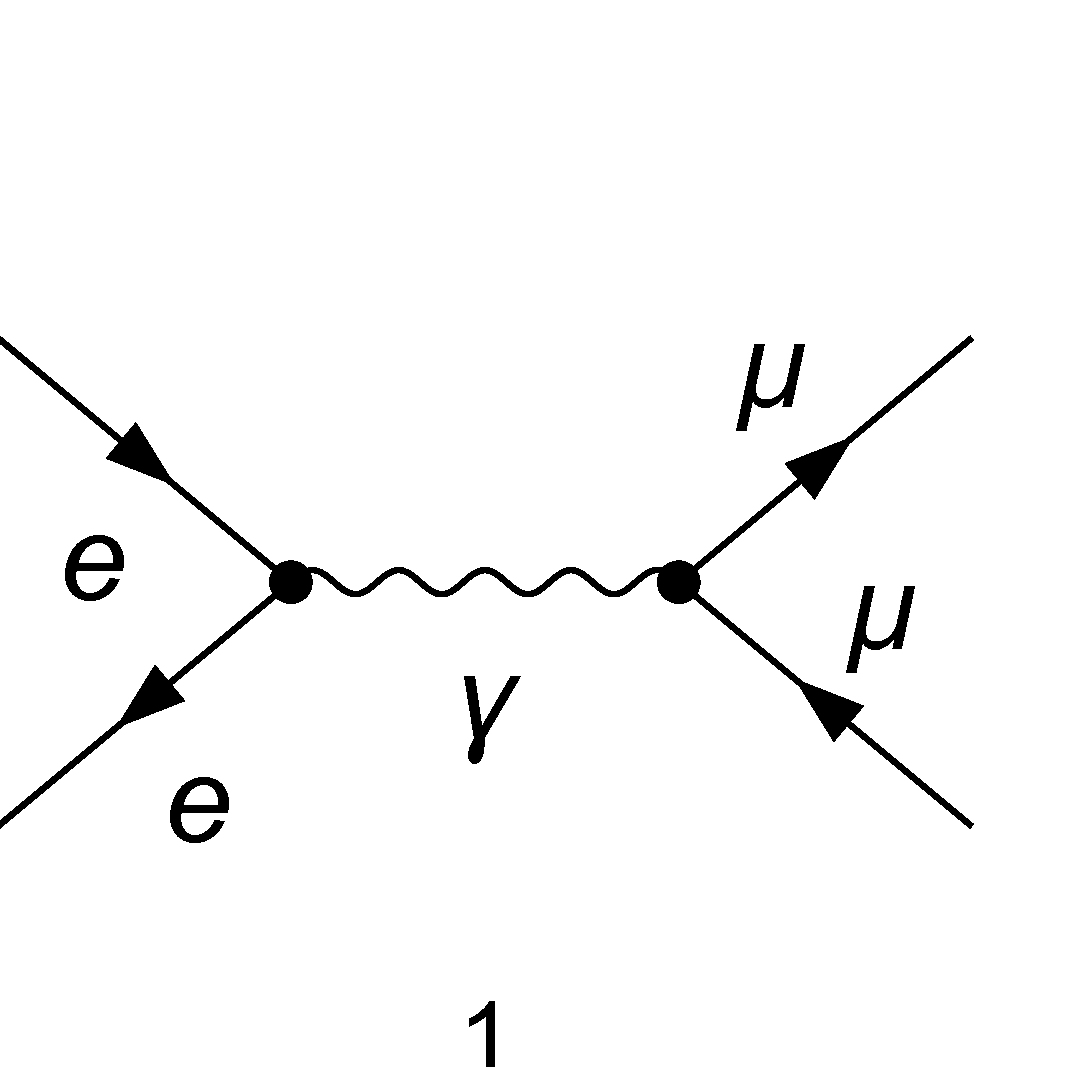
\includegraphics[width=0.8\textwidth]{images/feynart-fd-ee-mumu}
    \caption{The Feynman diagram generated by \textit{FeynArt}.}
    \label{fig:feynart result}
\end{figure}

We can turn this into the amplitude as follows:
\begin{lstlisting}[language=mathematica, gobble=4]
    amp[0] = FCFAConvert[CreateFeynAmp[diags],
        IncomingMomenta -> {p1, p2},
        OutgoingMomenta -> {p3, p4},
        UndoChiralSplittings -> True,
        ChangeDimension -> 4, List -> False, 
        SMP -> True, Contract -> True
    ]
\end{lstlisting}
here we use the \textit{FeynArt} function £CreateFeynAmp£ to create the Feynman amplitude and then the £FeynCalc£ function £FCFAConvert£ to turn the amplitude into a \textit{FeynCalc} compatible result.
This sets the momenta of the particles and does some simplifications.

Next we run £FCClearScalarProducts[]£ which just clears any defined values of scalar products, and is good practice to run at the start of each new calculation.
We can run the following commands:
\begin{lstlisting}[language=mathematica, gobble=4]
    MakeBoxes[p1, TraditionalForm] :=
        "\!\(\*SubscriptBox[\(p\),\(1\)]\)";
    MakeBoxes[p2, TraditionalForm] :=
        "\!\(\*SubscriptBox[\(p\),\(2\)]\)";
    MakeBoxes[p3, TraditionalForm] :=
        "\!\(\*SubscriptBox[\(p\),\(3\)]\)";
    MakeBoxes[p4, TraditionalForm] :=
        "\!\(\*SubscriptBox[\(p\),\(4\)]\)";
\end{lstlisting}
which just tell \textit{Mathematica} to pretty print £p1£ as \(p_1\) and so on.

Then we can run
\begin{lstlisting}[language=mathematica, gobble=4]
    SetMandelstam[s, t, u, p1, p2, -p3, -p4,
        SMP["m_e"], SMP["m_e"], SMP["m_mu"], SMP["m_mu"]]
\end{lstlisting}
The command
\begin{lstlisting}[language=mathematica, gobble=4]
    SetMandelstam[s, t, u, p1, p2, p3, p4,
        m1, m2, m3, m4]
\end{lstlisting}
sets the Mandelstam variables \(s = (p_1 + p_2)^2\), \(t = (p_1 + p_3)^2\), and \(u = (p_1 + p_4)^2\).
It also sets \(p_i^2 = m_i^2\).
Note that £SMP["par"]£ displays a parameter to the standard model, such as the mass of an electron, in a standard way.

Next we compute the amplitude squared:
\begin{lstlisting}[language=mathematica, gobble=4]
    ampSquared[0] = Simplify[DiracSimplify[
        (FermionSpinSum[#1, ExtraFactor -> 1/4] &)
        [FeynAmpDenominatorExplicit[amp[0]
        *ComplexConjugate[amp[0]]]]
    ]]
\end{lstlisting}
This squares the amplitude, computing \(\amplitude \amplitude^*\), then sums over the helicities with £FermionSpinSum£, manually including the factor of \(1/4\) from averaging over initial helicity states.
We then use \textit{FeynCalc}'s £DiracSimplify£ to simplify the spinor part and then \textit{Mathematica}'s £Simplify£ to simplify the normal algebra.
The result is
\begin{equation*}
    \frac{8e^4[m_{\symrm{e}}^2(p_3 \cdot p_4) + m_{\text{μ}}^2(p_1 \cdot p_2) + (p_1 \cdot p_4)(p_2 \cdot p3) + (p_1\cdot p_3)(p_2 \cdot p_4) + 2m_{\symrm{e}}^2m_{\text{μ}}^2]}{[2(p_3 \cdot p_4) + p_3^2 + p_4^2]^2}.
\end{equation*}

Now we make the approximation that the particle masses are negligible, which we do through
\begin{lstlisting}[language=mathematica, gobble=4]
    ampSquaredMassless[0] = Simplify[
        (#1/.{SMP["m_e"] -> 0, SMP["m_mu"] -> 0} &)
        [ampSquared[0]]
    ]
\end{lstlisting}
giving the result
\begin{equation}
    \frac{2e^4(t^2 + u^2)}{s^2}.
\end{equation}

Next we use the approximations
\begin{equation}
    t \approx -\frac{s}{2}(1 - \cos\vartheta), \qqand u \approx -\frac{s}{2} (1 + \cos\vartheta)
\end{equation}
where \(\vartheta\) is the scattering angle.
This holds in the high energy regime.
We also replace the electron charge, \(e\), with the fine structure constant.
To calculate the differential cross section we need two components, the prefactor and the bit that needs to be integrated to get the total cross section, we define these as
\begin{lstlisting}[language=mathematica, gobble=4, mathescape]
    prefactor = 1 / (64 $\pi^2$ s);
    integral = Factor[ampSquaredMassless[0] /.
        {t -> (-s/2)(1 - Cos[$\vartheta$]),
            u -> (-s/2)(1 + Cos[$\vartheta$]),
            SMP["e"]^4 -> (4$\pi$ SMP["alpha_fs"])^2}
    ]
\end{lstlisting}
This gives the result
\begin{equation}
    16 \pi^2 \alpha^2(1 + \cos^2\vartheta).
\end{equation}
The differential cross section is then
\begin{lstlisting}[language=mathematica, gobble=4, mathescape]
    differentialCrossSection = prefactor * integral
\end{lstlisting}
giving
\begin{equation}
    \diffp{\sigma}{\Omega} = \frac{\alpha^2}{4s}(1 + \cos^2\vartheta).
\end{equation}
To calculate the total cross section we can do the \(\varphi\) integral by hand, giving a factor of \(2\pi\), and then we have
\begin{lstlisting}[language=mathematica, gobble=4, mathescape]
    2$\pi$ Integrate[
        differentialCrossSection * Sin[$\vartheta$], {$\vartheta$, 0, $\pi$}
    ]
\end{lstlisting}
which gives the result
\begin{equation}
    \sigma = \frac{4\pi \alpha^2}{3s}.
\end{equation}
This is exactly the result found in \cref{chap:electron-positron to muon-antimuon}.
    \end{appendices}
    
    \backmatter
    \begin{thebibliography}{9}
        \bibitem{thomson} Thomson, M.\@ \textit{Modern Particle Physics}, (2013, Cambridge University Press, Cambridge)
        \bibitem{bartel} Bartel, W.\@ et al.\@ \textit{New Results on \(\APe\Pe\to\APmu\Pmu\) from the {JADE} Detector at {PETRA}}, Z.\@ Phys.\@ C, \textbf{26} December 1985 \href{https://doi.org/10.1007/BF01551792}{10.1007/BF01551792}
        \bibitem{bacino} Bacino, W.\@ et al.\@ \textit{Measurement of the Threshold Behavior of \(\APtau\Ptau\) Production in \(\APe\Pe\) Annihilation}, Phys.\@ Rev.\@ Lett., \textbf{41} 1 July 1938 \href{https://www.doi.org/10.1103/PhysRevLett.41.13}{10.1103/PhysRevLett.41.13}
        \bibitem{ball} Ball, R.\@ et al.\@ \textit{The Path to Proton Structure at One-Percent Accuracy}, Eur.\@ Phys.\@ J.\@ C \textbf{82} 428 11 May 2022 \href{https://doi.org/10.1140/epjc/s10052-022-10328-7}{10.1140/epjc/s10052-022-10328-7}
        \bibitem{higgsDiscovery} ATLAS experiment at CERN \url{https://cds.cern.ch/record/1459545} (Accessed 2022-11-26)
    \end{thebibliography}
    \renewcommand{\glossaryname}{Acronyms}
    \printglossary[acronym]
    \printindex
\end{document}